
%-------------------------------------------------------------------------------
%---------------------------Define Document Class and Packages------------------
%-------------------------------------------------------------------------------
\documentclass[10 pt]{book}

%  Standard packages
\usepackage{graphics,overcite,graphicx, amsmath, color}

%  for making index, using landscape mode, for multi page tables, supertabular??
\usepackage{makeidx, lscape, longtable, supertabular,}

%  Used for drawing lines in figures
\usepackage{ epic}

%  for showing script lines as they appear in GMAT
\usepackage{verbatim}

%  for using multicolumn format
\usepackage{multicol}

% Used for compact enumeration
\usepackage[pointedenum]{paralist}

% Used for writing algorithms
\usepackage{algorithm2e}

% Used for subscripts that use multiple lines

% for creating bookmarks in the final pdf file
\usepackage[ dvips, bookmarks = true, bookmarksopen = false ]{hyperref}
\usepackage{tocloft}
% for typesetting pseudo-code
%\usepackage{program}  - can't use right now due to conflict with
% command created below called \br

%-------------------------------------------------------------------------------
%---------------------------Define  the Page Size-------------------------------
%-------------------------------------------------------------------------------
\oddsidemargin  0.0in
\evensidemargin 0.0in
\textwidth      6.5in
\headheight     0.25in
\topmargin      -0.25in
\textheight     = 9.0in
%\setlength{\parskip}{8pt}

%-------------------------------------------------------------------------------
%------------------------------------New Commands-------------------------------
%-------------------------------------------------------------------------------
\newcommand{\st}[1]{\begin{ttfamily}#1\end{ttfamily}}      % transpose operator
\newcommand{\boldst}[1]{\begin{ttfamily}\textbf{#1} \end{ttfamily}}
\newcommand{\br}[0]{$\mathbf{r} $}
\newcommand{\bv}[0]{$\mathbf{v} $}
\newcommand{\ba}[0]{$\mathbf{a} $}
\newcommand{\mbr}[0]{\mathbf{r} }
\newcommand{\mbv}[0]{\mathbf{v} }
\newcommand{\mba}[0]{\mathbf{a} }
\newcommand{\mcR}[0]{\mathcal{R}}
\newcommand{\mcA}[0]{\mathcal{A}}
\newcommand{\mcB}[0]{\mathcal{B}}
\newcommand{\mcI}[0]{\mathcal{I}}
\newcommand{\mcS}[0]{\mathcal{S}}
\newcommand{\mcF}[0]{\mathcal{F}}
\newcommand{\mcO}[0]{\mathcal{O}}
\newcommand{\mcP}[0]{\mathcal{P}}
\newcommand{\mcT}[0]{\mathcal{T}}
%-------------------------------------------------------------------------------
%------------------------------------New Evironments----------------------------
%-------------------------------------------------------------------------------

\newenvironment{ScriptType}
  {\noindent \begin{ttfamily}   }
   { \end{ttfamily} }


\newenvironment{Script}
 { \vspace{-.15 in} \begin{ttfamily} }
 { \end{ttfamily}\vspace{-.25 in} }

%-------------------------------------------------------------------------------
%------------------------------------Miscellaneous------------------------------
%-------------------------------------------------------------------------------

\makeindex
%\let\package\textsf
%\let\env\textsf
\providecommand\finalclearpage{\clearpage}
%\setcounter{secnumdepth}{2} \rotdriver{dvips}

%  Make the watermark
\usepackage{eso-pic}
\usepackage{color}
\usepackage{type1cm}
\makeatletter
\AddToShipoutPicture{
    \setlength{\@tempdimb}{.5\paperwidth}%
    \setlength{\@tempdimc}{.5\paperheight}%
    \setlength{\unitlength}{1pt}%
    \put(\strip@pt\@tempdimb,\strip@pt\@tempdimc){%
    \makebox(0,720){\rotatebox{0}{\textcolor[gray]{0.75}
    {\fontsize{1.2cm}{1.2cm}\selectfont{Draft for Release R2016a}}}}
    }
} \makeatother


%-------------------------------------------------------------------------------
%------------------------------------Begin The Doc!!----------------------------
%-------------------------------------------------------------------------------
\begin{document}


%  Here we define the style for the bib.
\bibliographystyle{aiaa}
\thispagestyle{empty}

%%------------------------------------------------------------
%%-----------------Cover Page and TOC-------------------------
%%------------------------------------------------------------

\begin{center}
{\renewcommand{\thefootnote}{\fnsymbol{footnote}} { \Huge \bf
General Mission Analysis Tool\\ (GMAT)\\ Mathematical Specifications
}}
\end{center}
\begin{center}
{\renewcommand{\thefootnote}{\fnsymbol{footnote}} { \Huge \bf
 DRAFT }}
\end{center}

\begin{figure*}[htb]
\centering \centerline{
\begin{picture}(380,470)
\special{psfile= Images/GMATSplash.eps hoffset= 0 voffset= 0
hscale=60 vscale=60}
\end{picture}}
\end{figure*}
\vspace{-.2 in}
\begin{center}
\Large{NASA Goddard Space Flight Center\\
Greenbelt RD\\
Greenbelt, MD 20771}
\end{center}

\clearpage \clearpage

\tableofcontents \clearpage

 \listoffigures \clearpage

\listoftables

%\chapter{Introduction}
%\twocolumn

%------------------------------------------------------------
%-----------------Part I:  Mathematical Specifications-------
%------------------------------------------------------------

\chapter{Time } \label{Ch:TimeSystems} \index{Time systems}

Time is the primary independent variable in GMAT.  Time is used in
integrating the equations of motion, and calculating planetary
ephemerides, the orientations of planets and moons, and atmospheric
density among others.  GMAT uses three types of time systems
depending on the type of calculations being performed: universal
time systems based on the Earth's rotation with respect to the Sun;
dynamic time systems that are based on the dynamic motion of the
solar system and take into account relativistic effects; and atomic
time systems based on the oscillation of the cesium atom. Each of
these time systems has specific uses and is discussed below.  In
addition,  universal, dynamic, and atomic time systems can be
expressed in different time formats.  The two time formats used in
GMAT are the Modified Julian Date (MJD) format, and the Gregorian
Date (GD) format.  In the next section, we'll take a look at the
time systems used in GMAT, and when GMAT uses each time system. Then
we'll look at the different time formats.

\section{Time Systems}

GMAT uses several different time systems in physical models and
spacecraft dynamics modelling.  The choice of time system for  a
particular calculation is determined by which time system is most
natural and convenient, as well as the  accuracy required.  In
general, for determining Earth's orientation at a given epoch, we
use one of several forms of Universal Time (UT), because universal
time is based on the Earth's rotation with respect to the Sun.
Planetary ephemerides are usually provided with time in a dynamic
time system, because dynamic time is the independent variable in the
dynamic theories and ephemerides.  The independent variable in
spacecraft equations of motion in GMAT is time expressed in an
atomic time system.  Let's look at each of these three systems,
starting with atomic time.

\subsection{Atomic Time:  TAI and A.1} \index{Time systems!TAI}
\index{Time systems!A.1} \label{Sec:AtomicTime}

Atomic time (AT) is a highly accurate time system which is
independent of the rotation of the Earth\cite{vallado2}.
Therefore, AT is a natural system for integrating a spacecraft's
equations of motion.  AT is defined in terms of the oscillations
of the cesium atom at mean sea level. The duration of the SI
second is defined to be 9,192,631,770 oscillations of the cesium
nuclide 133Ce. Two atomic times systems are are used in GMAT: A.1,
and international atomic time (TAI). A.1 is in advance of TAI by
0.0343817 seconds.
%
\begin{equation}
     A.1 = TAI + 0.0343817 sec
\end{equation}
%
where
%
\begin{equation}
   TAI = UTC + \Delta AT
\end{equation}
%
and $\Delta AT$ is the number of leap seconds, added since 1972,
needed to keep $\mid UTC - UT1 \mid \leq 0.9 $sec.  GMAT reads
$\Delta AT$ from the file named \emph{tai-utc.dat}. For times that
appear before the first epoch on the file, GMAT uses the first value
found in the file.  For times that appear after the last epoch, GMAT
uses the last value contained in the file.  Currently, GMAT uses A.1
time as the independent variable in the equations of motion. TAI is
used as a time system for defining spacecraft state information.

Now let's look at the universal time system.


\subsection{Universal Time: UTC and UT1}\index{Time systems!UTC}
\index{Time systems!UT1} \label{Sec:UniversalTime}

All of the universal time (UT) scales are based on the Earth's
rotation with respect to a fixed point (sidereal time) or with
respect to the Sun (solar time). The observed universal time (UTO)
is determined from observations of stellar transits to determine
mean local sidereal time. UT1 is UTO corrected for the Earth's polar
motion and is used when the instantaneous orientation of the Earth
is needed.  UTC is the basis for all civil time standards. It is
also known as Greenwich mean time (GMT) and Zulu time (Z). The UTC
time unit is defined to be an SI second, but UTC is kept within 0.9
seconds of UT1 by occasional leap second adjustments.  The equation
relating UTC and UT1 is
%
\begin{equation}
    UTC = UT1 - \Delta UT1 \label{Eq:UT1ToUTC}
\end{equation}
%
In GMAT,  $\Delta UT1$ is read from the file \emph{eopc04.62-now}
provided by the International Earth Rotation and Reference Systems
Service (IERS). The file containing the latest measurements and
predictions can be found at
\\\emph{http://www.iers.org/}. For times past the last epoch
contained in the file, GMAT uses the last value of $ \Delta UT1$
contained in the file. GMAT uses UTC as a time system to define
spacecraft state information. UT1 is used to determine the Greenwich
hour angle and for the sidereal time portion of FK5 reduction.

\subsection{Dynamic Time: TT, TDB and TCB}\index{Time systems!TDB}
\index{Time systems!TT}\index{Time systems!TCB}
\label{Sec:DynamicTime}

Dynamical time is the independent variable in the dynamical
theories and ephemerides. This class of time scales contains
terrestrial time (TT),  Barycentric Dynamical time (TDB), and
Barycentric Coordinate Time (TCB).    TDB is the independent
variable in the equations of motion referred to the solar system
barycenter. It is also the coordinate time in the theory of
general relativity. Despite the fact that the Jet Propulsion
Laboratory (JPL) J2000.0 ephemerides are referred to in TDB, TT is
frequently used. This is because TT and TDB always differ by less
than 0.002 sec. As higher accuracy or more sensitive missions are
planned, the difference may need to be distinguished.  In this
section we'll discuss how to calculate TT, TDB and TCB, and
discuss where each is used in GMAT.

TT is the independent variable in the equations of motion referred
to the Earth's center. It is also the proper time in the theory of
general relativity. The unit of TT is a day of 86400 SI seconds at
mean sea level.  In GMAT, TT is used in FK5 reduction, and as an
intermediate time system in the calculation of TDB and TCB.  TT
can be calculated from the following equation:
%
\begin{equation}
     TT = TAI + 32.184 \hspace{.05 in}\mbox{sec}
\end{equation}
%

Calculating TDB exactly is a complicated process that involves
iteratively solving a transcendental equation.  For this reason,
it is convenient to use the following approximation
%
\begin{equation}
     TDB \approx TT + \underbrace{0.001658\sin{M_E} +
     0.00001385\sin{2M_E}}_{\mbox{units of seconds}}
\end{equation}
%
Note that the term in the underbrace has units of seconds, and
depending upon the units of $TT$, which is usually in days, a
conversion of the term may be necessary before performing the
addition with $TT$. $M_E$ is the Earth's mean anomaly with respect
to the sun and is given approximately as
%
\begin{equation}
     M_E \approx 357.5277233 + 35,999.05034 T_{TT}
\end{equation}
%
where $T_{TT}$ is the time in TT expressed in the Julian Century
format.  $T_{TT}$ can be calculated from
%
\begin{equation}
     T_{TT} = \frac{JD_{TT} - 2,451,545.0}{36,525} \label{Eq:T_TTComputation}
\end{equation}
%
where $JD_{TT}$  is the time in TT expressed in the Julian Date
format.  For a more complete discussion of the TDB time system, see
Vallado\cite{vallado2} (pp. 195-198) and Seidelmann\cite{seidelmann}
(pp. 41-48).  GMAT uses TDB as the default time system in the JPL
ephemerides files. There is an option to use TT in the ephemerides
using the \st{UseTTForEphemeris} flag.

The last dynamic time system GMAT uses is Barycentic Coordinate
Time.  In 1992, the IAU adopted this system and clarified the
relationships between space-time coordinates\cite{seidelmann}.  In
general, calculating TCB requires a four-dimensional space-time
transformation that is well beyond the scope of this discussion.
However, TCB can be approximated using the following equation:
%
\begin{equation}
 TCB - TDB = L_B  (JD - 2443144.5)  86400
 \end{equation}
%
The present estimate of the value of $L_B$ is $1.550505 x 10^{-8}$
$(+/- 1 x 10^{-14})$ (Fukushima et al., Celestial Mechanics, 38,
215, 1986).  It is important to note that the main difference
between TDB and TCB is a secular drift, and that as of the J2000
Epoch, the difference was approximately 11.25 seconds and growing
\cite{Seidelmann:etal:92}. GMAT uses time in the TCB system to
evaluate the IAU data  for the spin axes and prime meridian
locations of all planets and moons except for
Earth.\cite{Seidelmann:etal:02}  Note that
Seidelmann\cite{Seidelmann:etal:02} mistakenly says that time in TCB
should be used in the equations given for the  pole and meridian
locations of the planets.  The correct time to use is TDB, and GMAT
uses this time system.

\section{Time Formats} \index{Time Formats} \label{Sec:TimeFormats}

There are two time formats that GMAT uses to represent time in the
systems discussed above.  These formats are called the Gregorian
Date (GD), and the Julian Date (JD).  The difference between the GD
and JD formats is how they represent the Year, Month, Day, Hours,
Minutes, and Seconds of a given date.  The GD format is well known,
and the J2000 epoch is expressed as, 01 Jan 2000 12:00:00.000 TT.
The reference epoch for the GD calendar is the beginning of the
Christian Epoch.  The JD format represents an epoch as a continuous
number containing the day and the fraction of day.

The J2000 epoch \index{J2000 Epoch} is commonly used in
astrodynamics as a reference epoch for planetary and other data. The
J2000 epoch occurred at 01 Jan 2000 12:00:00.000 TT.  The time
system, TT, is important for precise applications!  While the J2000
epoch is a specific instant in time, the numerical value changes
depending upon which time system you express it in. We can make an
analogy with vector algebra where we have an abstract quantity that
is a vector, and can't write down a set of numbers representing the
vector until we choose a coordinate system. Similarly, the J2000
epoch can be written in any of the different time systems and
formats. All of the following are equivalent definitions of the
J2000 Epoch:
%
\begin{eqnarray}
    2451545.0 & TT \nonumber \\
    2451544.9996274998411 & TAI \nonumber \\
    2451544.9992571294708 & UTC \nonumber\\
    2451544.9999999990686 & TDB \nonumber
\end{eqnarray}
%
\begin{eqnarray}
 & \mbox{01 Jan }   2000 \hspace{.1 in} 12:00:00.000000000 &\mbox{TT} \nonumber \\
& \mbox{01 Jan }  2000 \hspace{.1 in}   11:59:27.815986276  &\mbox{TAI} \nonumber \\
& \mbox{01 Jan }  2000 \hspace{.1 in} 11:58:55.815986276 &\mbox{UTC} \nonumber\\
 & \mbox{01 Jan }  2000 \hspace{.1 in} 11:59:59.999919534  &\mbox{TDB} \nonumber
\end{eqnarray}

In the next two sections we'll look at how to convert an epoch in a
given time system from the GD format to the JD format, and vice
versa.

\subsection{Julian Date and Modified Julian Date}\index{Time
formats!Julian date} \index{Time formats!modified Julian
date}\label{Sec:JDFormat}

The Julian date is a time format in which we can express a time
known in any of the Atomic, Universal or Dynamic time systems. The
Julian Date is composed of the Julian day number and the decimal
fraction of the current day.  Seidelmann\cite{seidelmann} (pp.
55-56) says ``The Julian day number represents the number of days
that has elapsed, at Greenwich noon on the day designated, since
...the epoch noon Jan 1 4713 B.C. in the Julian proleptic
calendar.  The Julian date (JD) corresponding to any instant is,
by simple extension to this concept, the Julian day number
followed by  the fraction of the day elapsed since the preceding
noon".

The fundamental epoch for most astrodynamic calculations is the
J2000.0 epoch\cite{seidelmann}.  This epoch is GD 01 Jan 2000
12:00:00.000 in the TT time system and is expressed as JD 2451545.0
TT. To convert between Julian Date format and Gregorian Date format,
GMAT uses Algorithm 14 from Vallado\cite{vallado2}
%
\begin{equation}
\begin{split}
    JD = 367Y - Int\left( \displaystyle\frac{ 7\left( Y + Int\left( \displaystyle\frac{M + 9}{12} \right) \right)}{4}
    \right)+ \\Int\left(\displaystyle\frac{275M}{9} \right) + D +
    1,721,013.5 + \frac{ \displaystyle\frac{ \displaystyle\frac{s}{60}+m}{60} + H}{24}
    \end{split}
\end{equation}
%
where $Y$ is the four digit year, $Int$ signifies real truncation,
and $M$, $D$, $H$, $m$ and $s$ are month, day, hour, minutes, and
seconds respectively. This equation is valid for the time period 01
Mar. 1900 to 28 Feb. 2100.

For numerical reasons it is often convenient to work in a Modified
Julian Date (MJD) format to ensure we can capture enough significant
figures using double precision computers.  In GMAT the MJD system is
defined as
%
\begin{equation}
     MJD = JD - 2,430,000.0
\end{equation}
%
where the reference epoch expressed in the GD format is 05 Jan 1941
12:00:00.000.  However, we must be careful in calculating the
Modified Julian Date, or we will lose the precision we are trying to
gain.  GMAT calculates the MJD as follows:
%
\begin{equation}
     \begin{split}
     \mbox{JDay} = & 367Y - Int\left( \displaystyle\frac{ 7\left( Y + Int\left( \displaystyle\frac{M + 9}{12} \right) \right)}{4}
    \right)+ \\ & Int\left(\displaystyle\frac{275M}{9} \right) + D +
    1,721,013.5
    \end{split}
\end{equation}
%
\begin{equation}
     \mbox{PartofDay} = \frac{ \displaystyle\frac{ \displaystyle\frac{s}{60}+m}{60} + H}{24}
\end{equation}
%
\begin{equation}
     \mbox{MJD} = (\mbox{JDay}- 2,430,000.0) + \mbox{PartofDay}
\end{equation}
%
The important subtlety is that we must subtract the MJD reference
from the JD, before we add the fraction of day, to avoid losing
precision in the MJD.

\subsection{Gregorian Date}\index{Time formats!Gregorian
date}\label{Sec:GregorianDateFormat}

The Gregorian Date format is primarily used as a time system in
which to enter state information in GMAT.  GD is not a convenient
time format for most mathematical calculations.  Hence, GMAT often
takes input in the GD format and converts it to a MJD format for
use internally.  The algorithm for converting from GD to JD is
taken from Vallado\cite{vallado2} and reproduced here verbatim.

\begin{equation}
\begin{array}{llll}
      & T_{1900} = \displaystyle\frac{JD - 2,415,019.5}{365.25}\\
      & \\
      & Year = 1900 + \mbox{TRUNC}(T_{1900}) \\
      & \\
      & LeapYrs = \mbox{TRUNC}((Year - 1900 - 1)(0.25))\\
      & \\
      & Days = (JD - 2,415,019.5) - \\
      & \hspace{.5 in}((Year - 1900)(365.0) +
               LeapYrs)\\
      & \\
      & \mbox{IF} Days < 1.0 \mbox{ THEN}
      \end{array}\nonumber
\end{equation}
%
\begin{equation}
     \begin{array}{llll}
      & \\
      & \hspace{.5 in} Year = Year - 1 \\
      &  \\
      & \hspace{.5 in} LeapYrs = \mbox{TRUNC}((Year - 1900 - 1)(0.25))\\
      & \\
      & \hspace{.5 in}Days = (JD - 2,415,019.5) - \\
      & \hspace{1 in}((Year - 1900)(365.0) +
               LeapYrs)\\
      & \\
      & \mbox{If (\emph{Year} Mod 4)} = 0 \mbox{ Then} \\
      & \\
      &  \hspace{.5 in} LMonth[2] = 29 \\
       \end{array}\nonumber
\end{equation}
%
\begin{equation}
     \begin{array}{llll}
      & DayofYr = \mbox{TRUNC}(Days) \\
      & \\
      & \mbox{Sum days in each month until}\\
      & \hspace{.5 in} \mbox{\emph{LMonth} + 1 summation} > \mbox{\emph{DayofYr}} \\
      & \\
      &  Mon = \# \mbox{ of months in summation} \\
      & \\
      &  Day = DayofYr - LMonth \mbox{ summation}\\
      & \\
      &  \tau = (Days - DayofYr)24\\
      &  \\
      &  h = \mbox{TRUNC}(Temp)\\
      &  \\
      &  min = \mbox{TRUNC}((Temp - h)60) \\
      &  \\
      &  s = \left( Temp - h - \displaystyle\frac{min}{60} \right)3600
      %
       \end{array}\nonumber
\end{equation}

\section{Conclusions}

In this chapter we looked at three time systems that GMAT uses to
perform internal calculations:  atomic time, universal time, and
dynamic time.  Atomic time is used to integrate spacecraft
equations of motion, while universal time is used to determine the
sidereal time and greenwhich hour angle for use in FK5 reduction.
Dynamic time systems are used in the JPL ephemerides and in the
IAU planetary orientation data.   Time, in any of these time
systems, are represented in two formats:  the Gregorian Date, and
Julian Date. We looked at how to convert between different time
systems, and between different time formats.

% $Id: CoordinateSystems.tex,v 1.1 2008/01/31 18:04:16 dconway Exp $
\chapter{\label{chapter:CoordinateSystems}Coordinate Systems}
\chapauthor{Darrel J. Conway}{Thinking Systems, Inc.}

\textbf{NOTE: This chapter currently contains the original design spec for the coordinate systems.
It needs to be reviewed against the current GMAT system, the figures need to be recreated, and some
of the text needs to be fitted into the rest of the design document.}

This chapter presents design guidelines for the coordinate system classes in the Goddard Mission
Analysis Tool (GMAT). It describes how the GMAT software implements the coordinate system math
described in the GMAT Mathematical Specifications\cite{mathSpec}. This description includes the
initial design for the classes that provide coordinate system support in GMAT. The interactions
between these classes and the rest of the GMAT system are also described.

\section{Introduction}

The Goddard Mission Analysis Tool (GMAT) is a multi-platform orbit simulator designed to support
multiple spacecraft missions flying anywhere in the solar system. GMAT is written in C++ and runs on
Windows, Macintosh and Linux computer systems. The tool provides an integrated interface to MATLAB,
a high level computing environment from the Mathworks, Inc\cite{MATLAB}. The GMAT graphical user
interface (GUI) is written using the wxWidgets GUI Toolkit\cite{wxWidgets}, an open source library
that compiles and runs under all of the target operating systems.

GMAT is an object-oriented system, using the full extent of the C++ language to implement the object
model that provides GMAT's functionality.  The first three builds of GMAT provided capabilities to
model orbits in the vicinity of the Earth, including detailed force modeling, impulsive
maneuvers, and parameter targeting using a differential corrector.  All of these capabilities can be
controlled either using either the GMAT graphical user interface or a custom scripting language
designed to simplify GMAT and MATLAB interactions. The fourth build of the system generalizes the
capabilities of GMAT modeling for other orbital regimes.

In order to model spacecraft trajectories in these regimes, GMAT needs to be able to represent the
spacecraft state and related quantities in coordinate systems that are convenient to each regime.
This document describes how these coordinate systems are implemented in the GMAT code.


\section{\label{sec:CSClassDescription}Coordinate System Classes}

Figure \ref{figure:HighLevelCSClasses} shows the core C++ classes (drawn using
Poseidon\cite{poseidon}) added to GMAT to provide support for coordinate systems in Build 4. The
coordinate system capabilities are provided by the incorporation of these classes into the GMAT base
subsystem\footnote{The GMAT code base consists of a set of classes that provide the core
functionality of the system, the {}``base'' subsystem, and classes that comprise the graphical user
interface, the {}``gui'' subsystem.  All of the classes described in this document are members of
the base subsystem, with the exception of the recommendations for changes to the panels on the
GUI.}.

\begin{figure}[htb]
\begin{center}
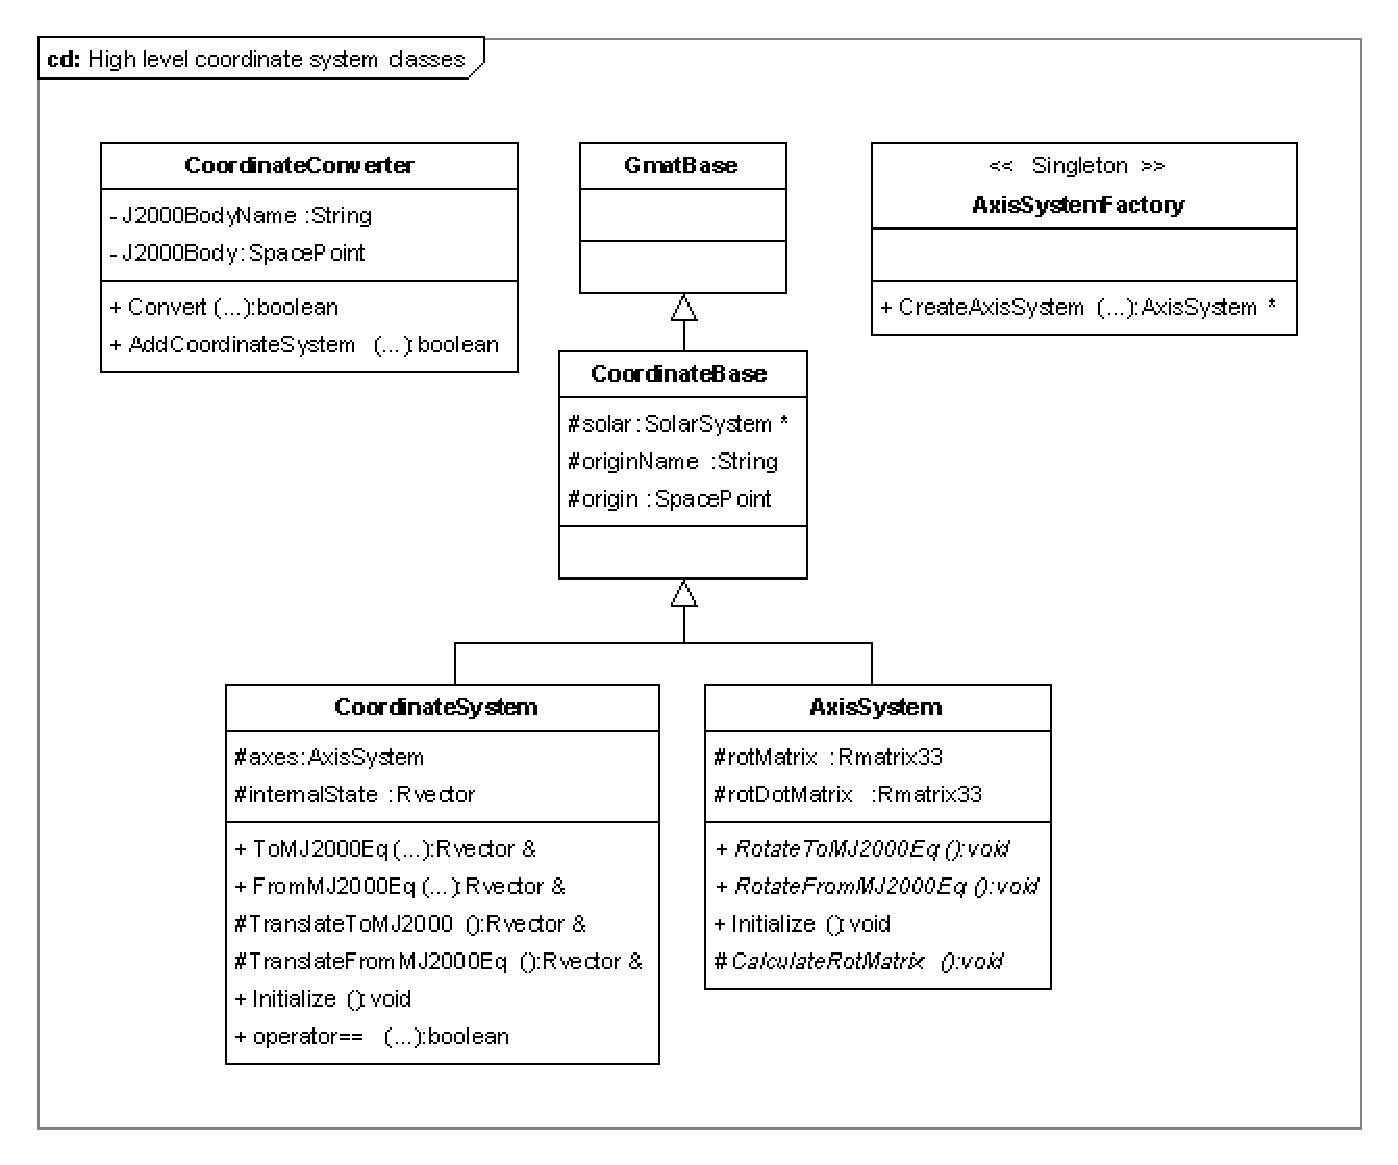
\includegraphics[scale=0.5]{Images/Highlevelcoordinatesystemclasses.eps}
\caption{\label{figure:HighLevelCSClasses}Coordinate System Classes in GMAT}
\end{center}
\end{figure}

The coordinate system classes consist of a CoordinateSystem class that acts as the interface between
the conversions and the rest of GMAT, an AxisSystem base class with a derived hierarchy used for
rotational conversions, a CoordinateConverter class that manages conversions between different
coordinate systems, and a factory constructed as a singleton that create the AxisSystem objects. The
CoordinateSystem class is the component that is instantiated when a user {}``Creates'' a coordinate
system object.

Previous builds of GMAT included classes that model spacecraft, formations, and celestial objects.
These classes were derived from a core base class named GmatBase. A new intermediate class,
SpacePoint, is implemented in GMAT to make access to position, velocity, and rotational data
available to the coordinate system classes when needed. Section~\ref{sub:SpacePointClassDescription}
describes this class.


\subsection{The CoordinateSystem Class}

The CoordinateSystem class is a configured component that implements the functionality needed to
convert into and out of a specified coordinate system. Internally, GMAT performs computations in a
Mean of J2000 Earth Equatorial coordinate system, centered at one of the celestial bodies in the
GMAT solar system (i.e. the Sun, a planet, or a moon) or at a barycenter or libration point. Each
CoordinateSystem instance provides methods to transform into and out of these J2000 coordinate
systems. It contains the data necessary for translation calculations, along with a member object
pointer that is set to an AxisSystem instance for coordinate systems whose principle axes are not
parallel to the Mean of J2000 Earth Equatorial axes, or to NULL for coordinate systems that are
oriented parallel to these axes.

The AxisSystem class provides the methods needed to rotate the coordinate system into and out of the
Mean of J2000 Earth Equator frame.  The AxisSystem is set for a given CoordinateSystem by setting
the axes member to an AxisSystem instance.

GMAT uses a late binding scheme to provide interconnections between objects used when modeling an
analysis problem. Individual components are configured from either the grapical user interface or a
script file describing the objects that need to be modeled. Connections between these objects are
defined using the names of the objects, but the actual object instances used in the model are not
set until the simulation is run. Upon execution, the configured objects are copied into the analysis
workspace, called the Sandbox, and the connections between the configured objects are established
immediately prior to the run of the simulation. The Initialize method in the CoordinateSystem class
implements this late binding for the connection between the coordinate system instance and the
related SpacePoints.


\subsection{The AxisSystem Class Hierarchy}

GMAT is capable of supporting numerous coordinate system orientations.  These orientations are
defined through the AxisSystem class; each unique axis orientation is implemented as a separate
class derived from the AxisSystem base class. Figure~\ref{figure:AxisSystemOverview} shows an
overview of the AxisSystem class hierarchy, and identifies the top level classes in this hierarchy.

\begin{figure}
\begin{center}
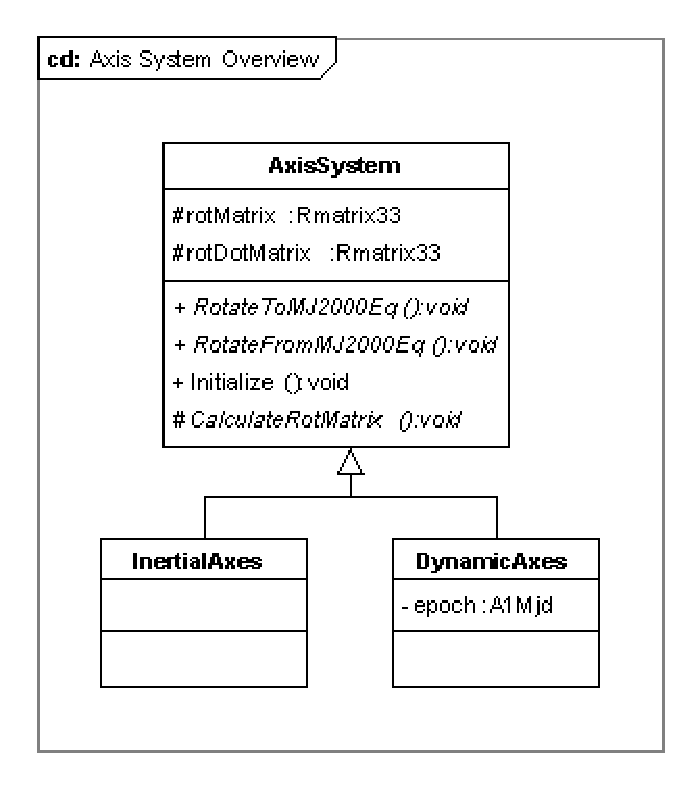
\includegraphics[scale=0.5]{Images/AxisSystemOverview.eps}
\caption{\label{figure:AxisSystemOverview}Top level AxisSystem Derived Classes}
\end{center}
\end{figure}

The orientations of the coordinate systems in GMAT fall into two broad categories: axes that change
orientation over time, and those that remain fixed in orientation. The latter category requires
computation of the rotation matrices one time, at initialization, in order to perform the rotations
into and out of the coordinate system.  Figure~\ref{figure:InertialAxisHierarchy} shows the six
inertial axis systems supported in GMAT. These systems support equatorial and ecliptic versions
of Mean of J2000, Mean of Epoch, and True of Epoch transformations.

\begin{figure}
\begin{center}
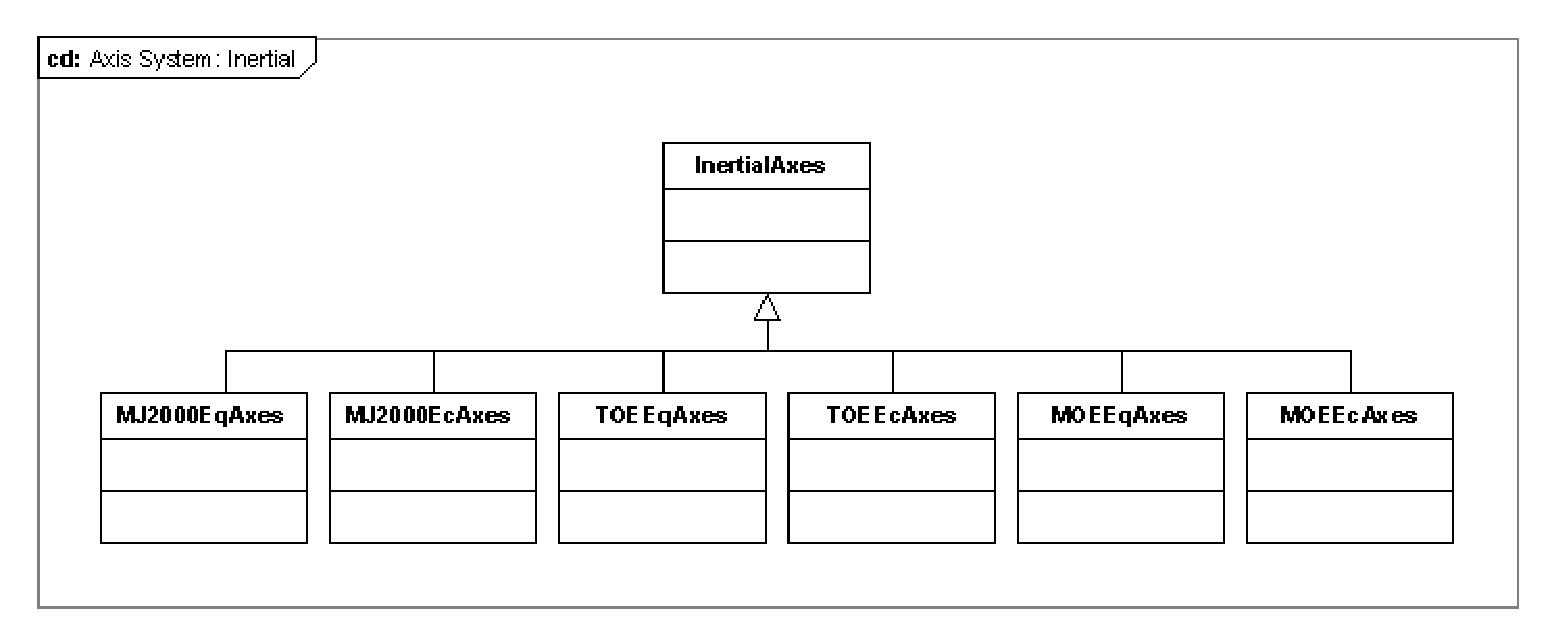
\includegraphics[scale=0.5]{Images/AxisSystemInertial.eps}
\caption{\label{figure:InertialAxisHierarchy}Inertial Axis Classes}
\end{center}
\end{figure}

Coordinate systems that are not fixed in orientation over time are derived from the DynamicAxes
class, as is shown in Figure~\ref{figure:DynamicAxisHierarchy}.  These coordinate systems include
equatorial and ecliptic versions of the mean of date and true of date axes, along with axes that
evolve with the polar motion of the body's rotational axis (implemented in the EquatorAxes class)
and axes that are fixed on the body's prime meridian (the BodyFixedAxes class). All of these classes
require recomputation of the orientation of the axes as the epoch of the model evolves.

\begin{figure}
\begin{center}
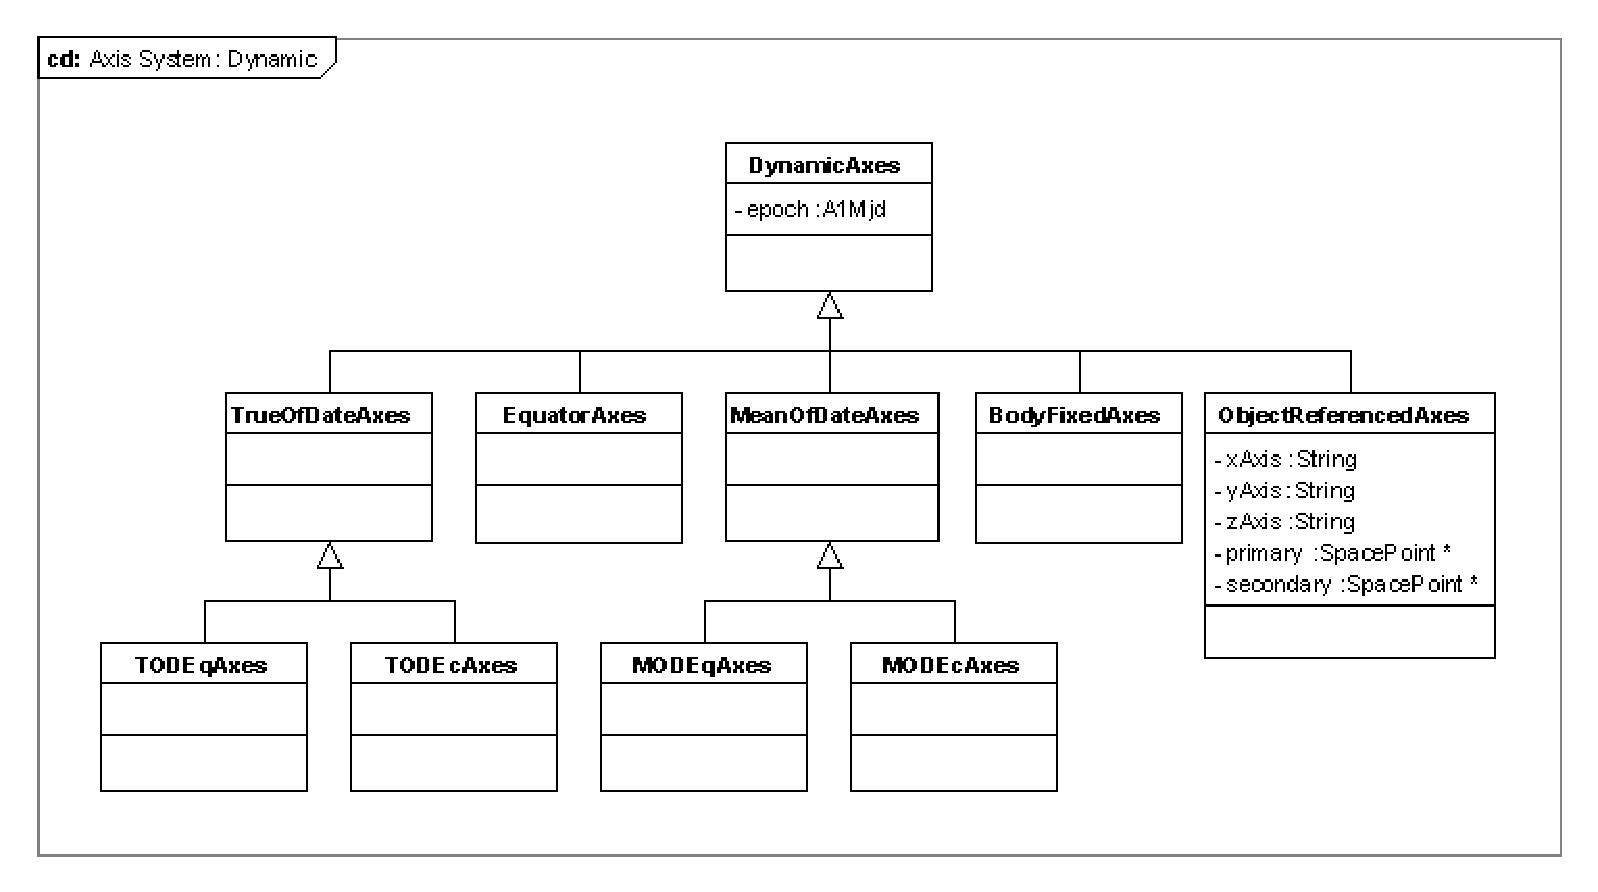
\includegraphics[scale=0.5]{Images/AxisSystemDynamic.eps}
\caption{\label{figure:DynamicAxisHierarchy}Dynamic Axis Classes}
\end{center}
\end{figure}

One additional class in Figure~\ref{figure:DynamicAxisHierarchy} bears discussion here. GMAT
supports numerous coordinate systems that reference bodies that are not celestial objects --
specifically coordinate systems that use Lagrange points, barycenters, spacecraft, and formations to
define the coordinate origins and axes. These coordinate systems use the ObjectReferencedAxes class
to construct the coordinate basis and rotation matrices. The GMAT Mathematical
Specifications\cite{mathSpec} provide detailed descriptions of how this class operates.

\subsection{CoordinateSystem and AxisSystem Collaboration}

The GMAT Mathematical Specification\cite{mathSpec} includes a flow chart that describes the
process of transforming between coordinate systems. This process is performed in the GMAT code using
the CoordinateConverter class and the public methods of the CoordinateSystem class. When GMAT needs
a conversion from one coordinate system to another, the method \texttt{CoordinateConverter::Convert}
is called with the epoch, input state, input coordinate system, output state, and output coordinate
system as parameters. The converted state vector is stored in the output state parameter.

The Convert method calls the conversion method \texttt{CoordinateSystem::ToMJ2000Eq} on the input
coordinate system, followed by \texttt{CoordinateSystem::FromMJ2000Eq} on the output coordinate
system. \texttt{ToMJ2000Eq} calls the \texttt{AxisSystem::RotateToMJ2000Eq} method followed by the
\texttt{Coordinate\-System::TranslateToMJ2000Eq} method, converting the input state from the input
coordinate system into Mean of J2000 Equatorial coordinates. Similarly, \texttt{FromMJ2000Eq} calls
the \texttt{Coordinate\-System::TranslateFromMJ2000Eq} method and then the
\texttt{AxisSystem::RotateFromMJ2000Eq} method, converting the intermediate state from Mean of J2000
Equatorial coordinates into the output coordinate system, completing the transformation from the
input coordinate system to the output coordinate system. Each of the conversion routines takes a
SpacePoint pointer as the last parameter in the call. This parameter identifies the J2000 coordinate
system origin to the conversion routine. If the pointer is NULL, the origin is set to the Earth.

The following paragraphs provide programmatic samples of these conversions.

\subsubsection{Code Snippets for a Conversion}

Figure~\ref{figure:TransformDetails}, generalized from the GMAT mathematical
specification, illustrates the procedure used to implement a transformation
from one coordinate system to another. The following paragraphs provide
code snippets with the corresponding function arguments for this process.

\begin{figure}
\begin{center}
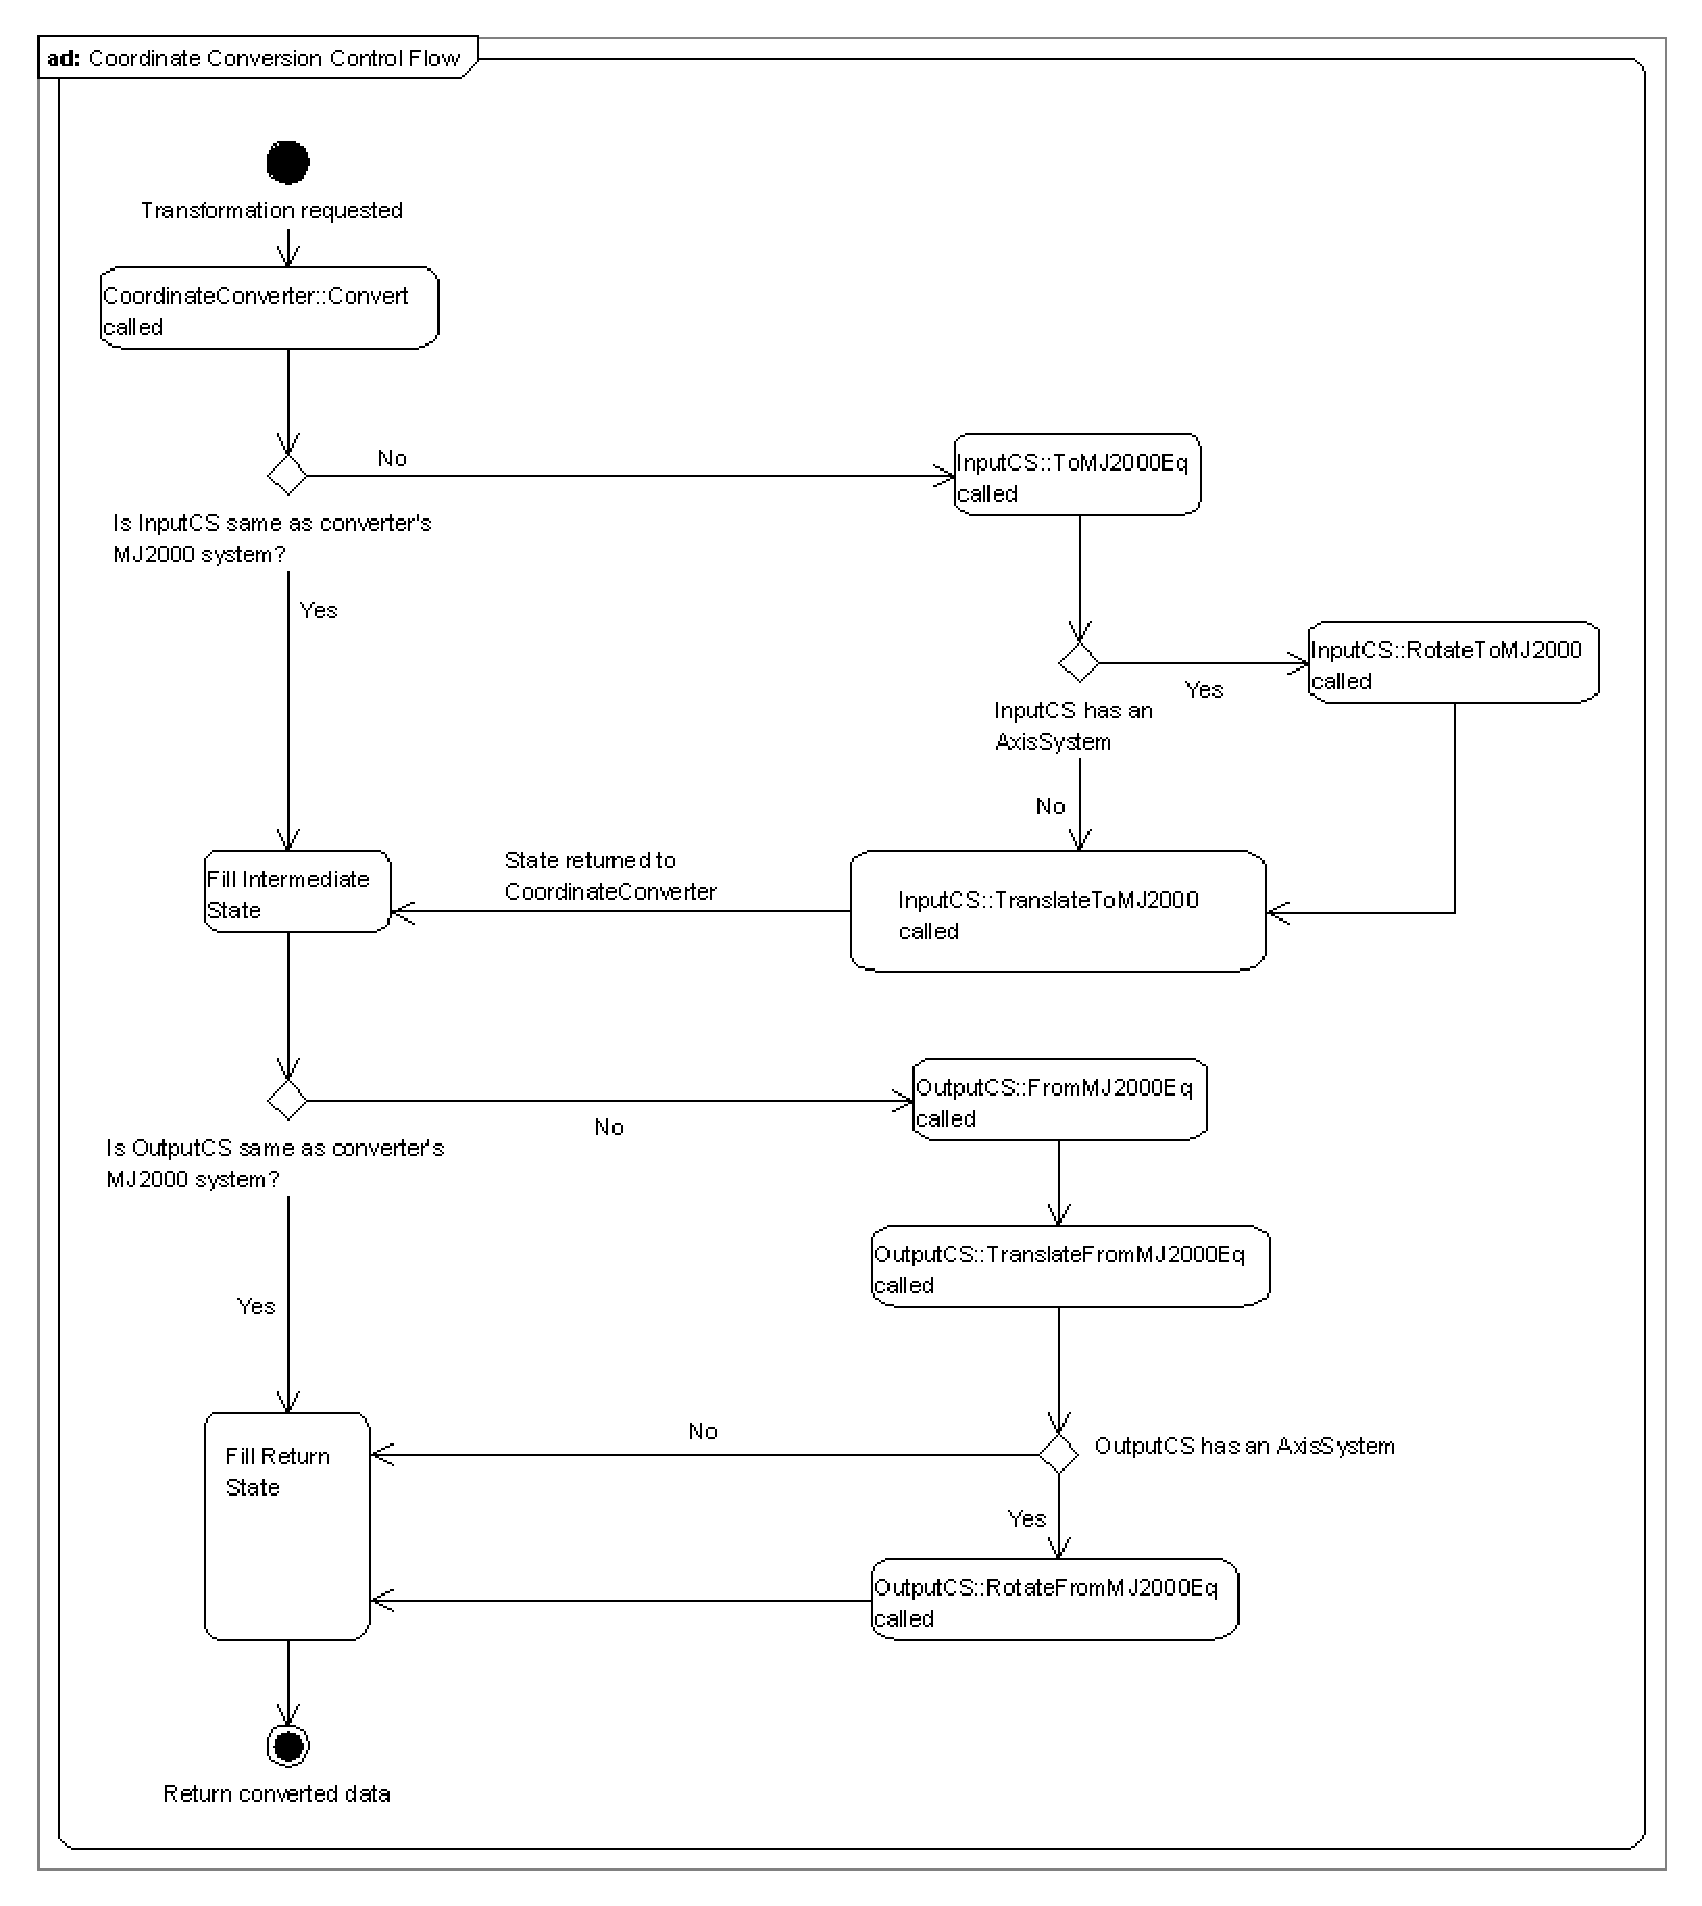
\includegraphics[scale=0.5]{Images/CoordinateConversionControlFlow.eps}
\caption{\label{figure:TransformDetails}GMAT Procedure for a Generic Coordinate Transformation}
\end{center}
\end{figure}

When GMAT needs to convert from one coordinate system to another, this method is called:

\begin{quotation}
\begin{verbatim}
if (!coordCvt->Convert(epoch, instate, inputCS, outstate, outputCS))
   throw CoordinateSystemException("Conversion from " +
      inputCS->GetName() + " to " + outputCS->GetName() + " failed.");
\end{verbatim}
\end{quotation}

This method invokes the calls listed above, like this:

\begin{quotation}
\begin{verbatim}
// Code in CoordinateConverter::Convert
if (!inputCS->ToMJ2000Eq(epoch, instate, internalState, J2000Body))
   throw CoordinateSystemException("Conversion to MJ2000 failed for " +
      inputCS->GetName());

if (!outputCS->FromMJ2000Eq(epoch, internalState, outState, J2000Body))
   throw CoordinateSystemException("Conversion from MJ2000 failed for " +
      outputCS->GetName());
\end{verbatim}
\end{quotation}

The conversion code from the input state to Mean of J2000 Equatorial
Coordinates is accomplished using the calls

\begin{quotation}
\begin{verbatim}
// Code in CoordinateSystem::ToMJ2000Eq
if (axes)      // axes == NULL for MJ2000Eq orientations
   if (!axes->RotateToMJ2000Eq(epoch, instate, internalState, J2000Body))
      throw CoordinateSystemException("Rotation to MJ2000 failed for " +
         instanceName);
else           // Set the intermediate state to the input state
   internalState = instate;

if (!TranslateToMJ2000Eq(epoch, internalstate, internalState, J2000Body))
   throw CoordinateSystemException("Translation to MJ2000 failed for " +
      instanceName);
\end{verbatim}
\end{quotation}

and the conversion from Mean of J2000 Equatorial Coordinates to the output state is performed using
these calls:

\begin{quotation}
\begin{verbatim}
// Code in CoordinateSystem::FromMJ2000Eq
if (!TranslateFromMJ2000Eq(epoch, internalstate, internalState, J2000Body))
   throw CoordinateSystemException("Translation from MJ2000 failed for " +
      instanceName);

if (axes)      // axes == NULL for MJ2000Eq orientations
   if (!axes->RotateFromMJ2000Eq(epoch, internalState, outstate, J2000Body))
      throw CoordinateSystemException("Rotation from MJ2000 failed for " +
         instanceName);
else           // Set the output state to the intermediate state
   outstate = internalState;
\end{verbatim}
\end{quotation}

\subsection{\label{sub:SpacePointClassDescription}The SpacePoint Class}

In general, coordinate systems are defined in reference to locations and directions in space. Many
of the coordinate systems used in GMAT have the direction fixed based on an external reference --
for example, the MJ2000Eq system has the z-axis pointed along the Earth's rotation axis at the J2000
epoch and the x-axis aligned with the vernal equinox at the same epoch. GMAT also supports
coordinate systems constructed in reference to objects internal to the GMAT -- typically a planet,
the Sun, a moon, or a spacecraft can be used, as can special points in space like Lagrange points or
the barycenter of a multi-body system.  The coordinate system classes need to be able to access
position and velocity data about these objects in a generic fashion. GMAT has a class, SpacePoint,
that provides this access. SpacePoint is the base class for all of the objects that model location
data in the solar system, as is shown in Figure~\ref{figure:SpacePointHierarchy}.  The SpacePoint
class is described in more detail in Chapter~\ref{chapter:SolarSystem}.

\begin{figure}
\begin{center}
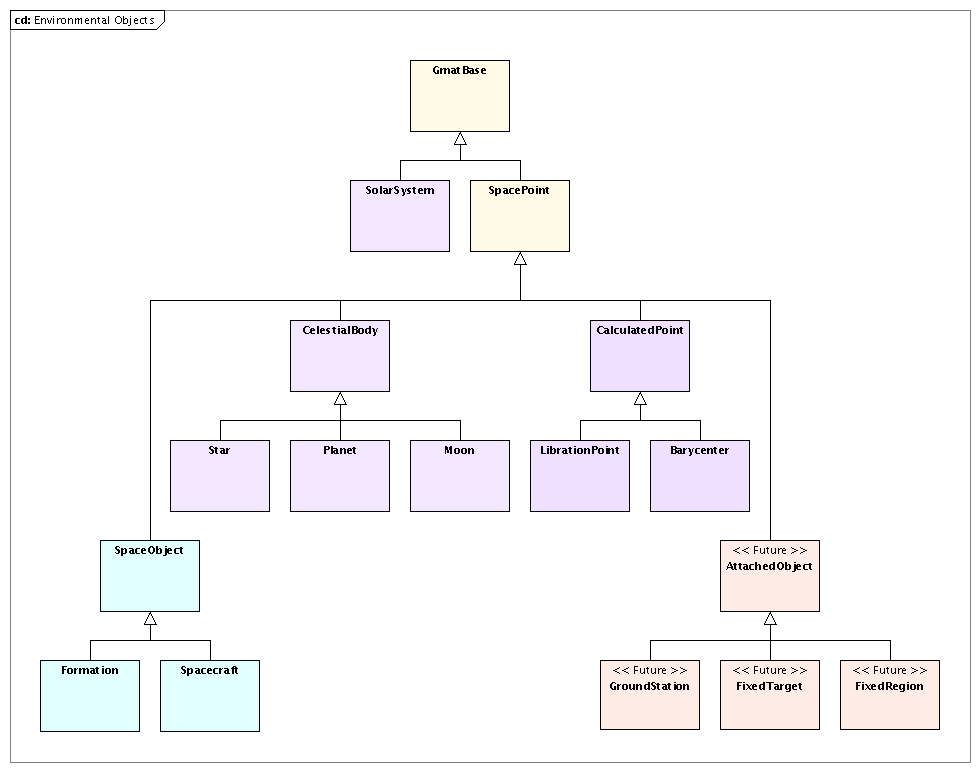
\includegraphics[scale=0.5]{Images/EnvironmentalObjects.eps}
\caption{\label{figure:SpacePointHierarchy}The SpacePoint Class Hierarchy}
\end{center}
\end{figure}

\section{\label{sec:CSScriptConfiguration}Configuring Coordinate Systems}

\subsection{Scripting a Coordinate System}

The script commands used to create a coordinate system object in GMAT are defined in the GMAT
Mathematical Specifications\cite{mathSpec}.  Coordinate System scripting is performed using the
following lines of script:

\begin{quotation}
\begin{verbatim}
Create CoordinateSystem csName
GMAT csName.Origin = <SpacePoint name>;
GMAT csName.Axes = <Axis type>;
GMAT csName.Primary = <Primary SpacePoint name, if needed>;
GMAT csName.Secondary = <Secondary SpacePoint name, if needed>;
GMAT csName.Epoch.<Format> = <Epoch data, if needed>;

% Only two of these three can exist for a given coordinate system;
% see the coordinate system table for more information
GMAT csName.XAxis = <$\pm$R, $\pm$V, or $\pm$N>;
GMAT csName.YAxis = <$\pm$R, $\pm$V, or $\pm$N>;
GMAT csName.ZAxis = <$\pm$R, $\pm$V, or $\pm$N>;
\end{verbatim}
\end{quotation}

The fields in angle brackets are used to set the parameters that define the coordinate system.
Table~\ref{table:CSParms} provides a brief description of these fields; more details are available
in \cite{mathSpec}.

%
\begin{table}
\caption{\label{table:CSParms}Coordinate System Parameters}
\begin{center}\begin{tabular}{|p{0.8in}|p{0.9in}|p{1.3in}|p{2.5in}|}
\hline
Parameter&
Required/ Optional&
Allowed Values&
Description\tabularnewline
\hline
\hline
Origin&
Required&
\begin{flushleft}Any Named SpacePoint\end{flushleft}&
Defines the location of the coordinate system origin.\tabularnewline
\hline
Axes&
Required&
\begin{flushleft}Equator, MJ2000Ec, MJ2000Eq, TOEEq, MOEEq, TODEq,
MODEq, TOEEc, MOEEc, TODEc, MODEc, Fixed, ObjectRefernced\end{flushleft}&
Defines the orientation of the coordinate axes in space.\tabularnewline
\hline
Primary&
Optional&
\begin{flushleft}Any Named SpacePoint\end{flushleft}&
Defines the primary body used to orient axes for systems that need
a primary body.\tabularnewline
\hline
Secondary&
Optional&
\begin{flushleft}Any Named SpacePoint\end{flushleft}&
Defines the secondary body used to orient axes for systems that need
a secondary body.\tabularnewline
\hline
Epoch&
Optional&
Any GMAT Epoch&
Sets the reference epoch for systems that need a reference epoch.\tabularnewline
\hline
XAxis&
Optional&
$\pm\textrm{R,}\pm\textrm{V,}\pm\textrm{N}$&
Used for ObjectReferences axes only; two of the three axes are set,
and one must reference $\pm N$.\tabularnewline
\hline
YAxis&
Optional&
$\pm\textrm{R,}\pm\textrm{V,}\pm\textrm{N}$&
Used for ObjectReferences axes only; two of the three axes are set,
and one must reference $\pm N$.\tabularnewline
\hline
ZAxis&
Optional&
$\pm\textrm{R,}\pm\textrm{V,}\pm\textrm{N}$&
Used for ObjectReferences axes only; two of the three axes are set,
and one must reference $\pm N$.\tabularnewline
\hline
\end{tabular}\end{center}
\end{table}

In the following paragraphs, the interactions between the script interpreter subsystem and the
coordinate system classes are described.

\subsubsection{Script Interpreter Actions}

In GMAT, the ScriptInterpreter reads each line of script and sets up the corresponding objects. The
lines of script above map to calls made in the ScriptInterpreter code, as described in the following
text.

The Create line causes the ScriptInterpreter to call the CoordinateSystemFactory and requests a
CoordinateSystem instance:

\begin{quotation}
\begin{verbatim}
// In the Interpreter subsystem
GmatBase *csInstance = moderator->CreateCoordinateSystem("CoordinateSystem", "csName");
\end{verbatim}
\end{quotation}

The resulting coordinate system is registered with the configuration manager.

The Origin line sets the originName parameter on this instance:

\begin{quotation}
\begin{verbatim}
// First determine that the parm is a string
Gmat::ParameterType type = csInstance->GetParameterType({}``Origin'');

// Here type is a string, so this is called:
csInstance->SetStringParameter({}``Origin'', <SpacePoint name>);
\end{verbatim}
\end{quotation}

The Axes line creates an instance of the AxisSystem and passes it to the coordinate system:

\begin{quotation}
\begin{verbatim}
// First determine that the parm is an internal object
Gmat::ParameterType type = csInstance->GetParameterType({}``Axes'');

// Here type is an object, so this is called:
GmatBase {*}axesInstance = moderator->CreateAxisSystem(<Axis type>, {}``'');

// Then the object is set on the coordinate system
csInstance->SetRefObject(axesInstance);
\end{verbatim}
\end{quotation}

The Primary line sets the primary body on the AxisSystem instance.  This is done by passing the data
through the CoordinateSystem object into the AxisSystem object:

\begin{quotation}
\begin{verbatim}
// First determine that the parm is a string
Gmat::ParameterType type = csInstance->GetParameterType({}``Primary'');

// Pass the string to the coordinate system
csInstance->SetStringParameter({}``Primary'', <SpacePoint name>);

...

// In CoordinateSystem, this parameter is passed to the AxisSystem:
axes->SetStringParameter({}``Primary'', <SpacePoint name>);
\end{verbatim}
\end{quotation}

The Secondary line is treated similarly to the primary line:

\begin{quotation}
\begin{verbatim}
// First determine that the parm is a string
Gmat::ParameterType type = csInstance->GetParameterType({}``Secondary'');

// Pass the string to the coordinate system
csInstance->SetStringParameter({}``Secondary'', <SpacePoint name>);

...

// In CoordinateSystem, this parameter is passed to the AxisSystem:
axes->SetStringParameter({}``Secondary'', <SpacePoint name>);
\end{verbatim}
\end{quotation}

The Epoch line is handled like in the Spacecraft object, and the XAxis, YAxis and ZAxis lines are
treated as string inputs, like the Primary and Secondary lines, above.

\subsection{Default Coordinate Systems}

GMAT defines several coordinate systems by default when it is initialized.  These systems are listed
in Table \ref{table:DefaultCSs}.

\begin{table}
\caption{\label{table:DefaultCSs}Default Coordinate Systems defined in GMAT}
\centerline{\begin{tabular}{|p{1in}|p{1in}|p{1.5in}|p{2in}|}
\hline
Name&
Origin&
Axis System&
Comments\tabularnewline
\hline
\hline
EarthMJ2000Eq&
Earth&
MJ2000 Earth Equator&
The default coordinate system for GMAT\tabularnewline
\hline
EarthMJ2000Ec&
Earth&
MJ2000 Ecliptic&
\tabularnewline
\hline
EarthFixed&
Earth&
Body Fixed&
The Earth fixed system is used by the gravity model for full field
modeling\tabularnewline
\hline
BodyFixed&
Other celestial bodies&
Body Fixed&
Fixed systems used by the gravity model for full field modeling at
other bodies\tabularnewline
\hline
\end{tabular}}
\end{table}

\section{Coordinate System Integration }

Sections \ref{sec:CSClassDescription} and \ref{sec:CSScriptConfiguration} describe the internal
workings of the GMAT coordinate systems, but do not explain how the coordinate system code interacts
with the rest of GMAT. This section outlines that information.


\subsection{General Considerations}

GMAT uses coordinate systems in several general areas: for the input of initial state data,
internally in the impulsive and finite burn code, force models and propagation code, in the
calculation of parameters used to evaluate the behavior of the model being run, and in the graphical
user interface (GUI) to display data as viewed from a coordinate system based perspective.

\subsection{Creation and Configuration}

\subsubsection{Coordinate System Creation}

Coordinate systems are created through a series of interactions between the GMAT interpreters, the
Moderator, and the Factory system. Figure~\ref{figure:CSCreationSequence} shows the sequence
followed by the ScriptInterpreter when a coordinate system is configured from a script.  The
procedure is similar when the GUI configures a coordinate system, with one exception. The
ScriptInterpreter translates a script file a line at a time, so it needs to look up the
CoordinateSystem object each time it is referenced in the script. The GUI configures the coordinate
system from a single panel, so the coordinate system object does not need to be found each time a
parameter is accessed.

\begin{figure}
\begin{center}
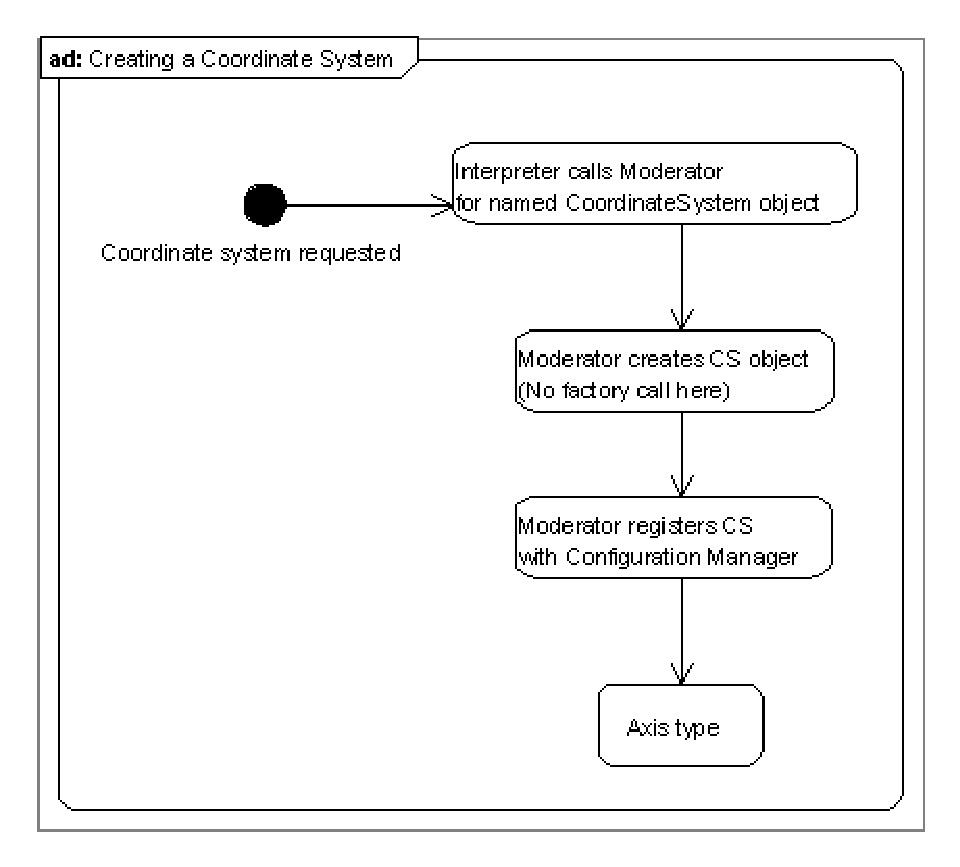
\includegraphics[scale=0.5]{Images/CSCreationSequence.eps}
\caption{\label{figure:CSCreationSequence}Coordinate System Creation and Configuration Sequence}
\end{center}
\end{figure}

\subsubsection{Startup Considerations}

When a user starts GMAT, the executable program creates a singleton instance of the Moderator. The
Moderator is the core control module in GMAT; it manages the creation and deletion of resources, the
interfaces between the core components of the system and the external interfaces (including the GUI
and the scripting engines), and the execution of GMAT simulations. When the Moderator is created, it
creates a variety of default resources, including the default factories used to create the objects
in a simulation. The factories that get created include the CoordinateSystemFactory.

After it has created the factories and constructed the default solar system, the Moderator creates
the default coordinate systems listed in Table \ref{table:DefaultCSs}, following a procedure like
the one shown in Figure \ref{figure:CSCreationSequence}. These coordinate systems are registered
with the Configuration Manager using the names in the table. Users can use these coordinate systems
without any taking any additional configuration actions.

\subsection{Sandbox Initialization}

When a user runs a mission sequence, the Moderator takes the following sequence of actions
\footnote{The description here references a Sandbox for the run. The Moderator can be configured to
manage a collection of Sandboxes; in that case, the actions described here are applied to the
current Sandbox from that collection.}:

\begin{enumerate}
\item Send the current SolarSystem to the Sandbox for cloning
\item Load the configured objects one at a time into the Sandbox. These objects are cloned
\footnote{The current build of GMAT does not fully implement cloning for the configured objects.
This issue is being corrected.} into the Sandbox.
\item The Sandbox is initialized.
\item The Mission is executed.
\end{enumerate}

\noindent The critical piece for successful execution of a GMAT mission is the third step. When the
Sandbox is initialized, the following actions are executed:

\begin{enumerate}
\item The local solar system object is set for all of the objects that need it.
\item Reference object pointers are set on objects that use them.
\item \label{enu:ObjectInit}The objects are initialized.
\item Parameters are configured.
\item The command sequence is configured.
\begin{enumerate}
\item The object table is passed to each command.
\item The solar system is passed to each command.
\item \label{enu:CS-CommandInit}The command is initialized.
\end{enumerate}
\end{enumerate}

\noindent The coordinate system objects are fully initialized and ready for use by the end of the
step \ref{enu:ObjectInit}. Commands that use the coordinate system objects have the object
associations set in step~\ref{enu:CS-CommandInit}.

\subsection{Initial States}

Users need to set the locations and initial motion of spacecraft, ground stations, and other
physical entities modeled in GMAT using a coordinate system that makes this data simple to specify.
For this reason, GMAT lets users select all or a portion of the coordinate system needed for these
objects.

\subsubsection{Spacecraft}

The initial state for a spacecraft is expressed as an epoch and six numerical quantities
representing the spacecraft's location and instantaneous motion. These quantities are typically
expressed as either six Cartesian elements -- the x, y, and z components of the position and
velocity, six Keplerian elements -- the semimajor axis, eccentricity, inclination, right ascension
of the ascending node, argument of pariapsis, and the anomaly in one of three forms (true, mean, or
eccentric), or one of several other state representations. The element representation depends on the
coordinate system used. Some representations cannot be used with some coordinate systems -- for
example, the Keplerian representation requires a gravitational parameter, $\mu=GM$, in order to
calculate the elements, so coordinate systems that do not have a massive body at the origin cannot
be used for Keplerian elements. For these cases, GMAT reports an error if the element type is
incompatible with the coordinate system.

\subsubsection{Ground Stations and Other Body Fixed Objects}

Ground station objects and other objects connected to physical locations on a body are expressed in
terms of the latitude, longitude, and height above the mean ellipsoid for the body. The coordinate
system used for these objects is a body fixed coordinate system. Users can specify the central body
when they configure these objects. The body radius and flattening factor for that body are used to
calculate the mean ellipsoid. Latitude is the geodetic latitude of the location, and longitude is
measured eastwards from the body's prime meridian.

GMAT does not currently support ground stations or other body fixed objects. This section will be
updated when this support is added to the system.

\subsection{Forces and Propagators}

Internal states in GMAT are always stored in a Mean of J2000 Earth-Equator coordinate system. The
origin for this system is set to either a celestial body (i.e. the Sun, a planet, or a moon), a
barycenter between two or more bodies, or a Lagrange point. The propagation subsystem in GMAT allows
the user to specify this origin, but no other coordinate system parameters. Propagation is performed
in the Mean of J2000 Earth-Equator frame located at the specified origin.

Individual forces in the force model may require additional coordinate system transformations. These
transformations are described in the next section.

\subsubsection{Coordinate Systems Used in the Forces }

GMAT contains models for point mass and full field gravity from both a central body and other
bodies, atmospheric drag, solar radiation pressure, and thrust from thrusters during finite
maneuvers. Table~\ref{table:ForceModelCoordinateSystems} identifies the coordinate system used for
each force. Users set the point used as the origin for the force model. This point is labeled
$\mathbf{r_{o}}$ in the table. Forces that require a central body reference that body as
$\mathbf{r_{cb}}$ in the table. Users also specify the coordinate system used for finite maneuvers.
All other coordinate systems are set up internally in the force model code, and managed by the
constituent forces.

\begin{table}
\caption{\label{table:ForceModelCoordinateSystems}Coordinate Systems Used by Individual Forces}
\centerline{\begin{tabular}{|p{1.5in}|>{\raggedright}p{1.5in}|p{3in}|}
\hline
Force&
Coordinate System&
Notes\tabularnewline
\hline
\hline
Point Mass Gravity&
$\mathbf{r_{o}}$ centered MJ2000 Earth Equator&
Point mass forces use the default representations\tabularnewline
\hline
Full Field Gravity&
$\mathbf{r_{cb}}$ centered Body Fixed&
Full field models use the body fixed system to calculate latitude
and longitude data, and calculate accelerations in the MJ2000 frame
based on those values.\tabularnewline
\hline
Drag&
$\mathbf{r_{cb}}$ centered MJ2000 Earth Equator&
Drag forces set the atmosphere to rotate with the associated body,
so the reference frame remains inertial (i.e. MJ2000 based).\tabularnewline
\hline
Solar Radiation Pressure&
$\mathbf{r_{o}}$ centered MJ2000 Earth Equator&
Solar Radiation Pressure calculations are performed in MJ2000 coordinates\tabularnewline
\hline
Finite Maneuver Thrust&
Any Defined Coordinate System, user specified&
Finite maneuvers determine the thrust direction based on the thrust vector associated with the
engines. The spacecraft are aligned with this coordinate system. A future build will add an
additional transformation to allow specification of the spacecraft's attitude in this
frame.\tabularnewline
\hline
\end{tabular}}
\end{table}

\subsubsection{Transformations During Propagation}

GMAT's propagators consist of a numerical integrator and an associated force model. Each force model
is a collection os individual forces that get added togehter to determine the net acceleration
applied to the object that is propagated. The preceding section defined the coordinate systems used
by each of these forces. Figure~\ref{figure:forceFlow} shows the procedure that is followed each
time the force model calculates the acceleration applied to an object.

\begin{figure}
\begin{center}
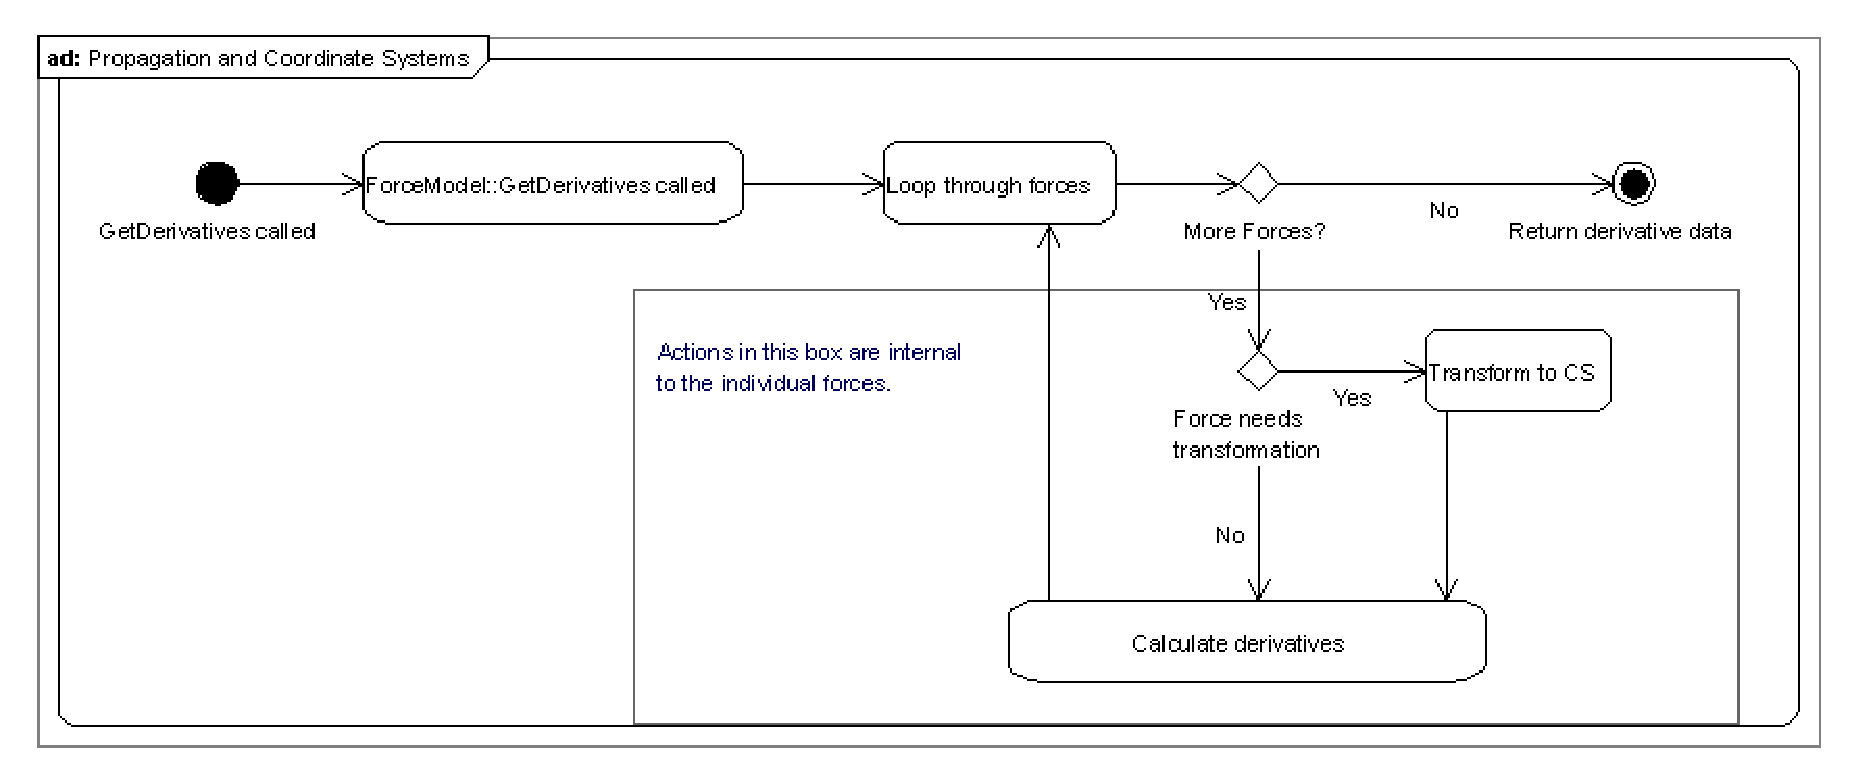
\includegraphics[scale=0.5]{Images/PropagationandCoordinateSystems.eps}
\caption{\label{figure:forceFlow}Control Flow for Transformations During Propagation}
\end{center}
\end{figure}

The force model calls each force in turn. As a force is called, it begins by transforming from the
internal Mean of J2000 equatorial coordinate system into the coordinate system required for that
force.  The acceleration from the force is then calculated.

\subsection{Maneuvers}

The impulsive and finite burn models are used to simulate thruster actions on a spacecraft.
Maneuvers are applied either as an impulsive delta-V or as an acceleration in the force model. In
either case, the coordinate system related operations in the maneuver object are the same: the basis
vectors for the coordinate system are calculated in the MJ2000 frame, the magnitude of the change in
the velocity is calculated for the maneuver (resulting in a delta-V magnitude for impulsive
maneuvers, or the time rate of change of velocity for finite maneuvers), and the resultant is
projected along the basis vectors using attitude data in the maneuver object.
Figure~\ref{figure:ManeuverFlow} illustrates this flow.

\begin{figure}
\begin{center}
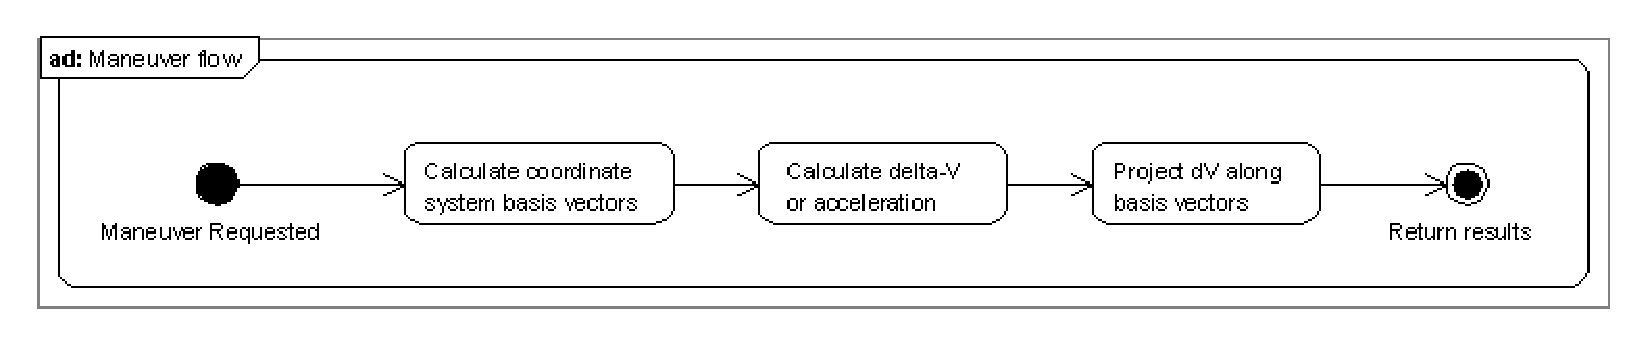
\includegraphics[scale=0.5]{Images/Maneuverflow.eps}
\caption{\label{figure:ManeuverFlow}Calculating the Direction Used for Maneuvers}
\end{center}
\end{figure}

\subsection{Parameters}

Many of the parameters that GMAT can calculate are computed based on the coordinate system of the
input data; in some cases this dependency uses the full coordinate system, and in other cases, it
uses the origin or central body of the coordinate system. The Parameter subsystem contains flags for
each parameter taht are used to indicate the level of coordinate system information required for
that parameter. These flags indicate if the parameter is specified independently from the coordinate
system, depends only on the origin of a coordinate system, or depends on a fully specified
coordinate system.

\subsection{Coordinate Systems and the GUI }

\subsubsection{\label{sub:OpenGLViewPoints}OpenGL ViewPoints}

The OpenGL visualization component in the first three GMAT builds set the Earth at the center of the
display view and allowed users to move their Earth-pointing viewpoint to different locations. The
incorporation of coordinate systems into the code opens GMAT to a greatly expanded visualization
capability in this component. Users can set the viewing direction to point towards any SpacePoint or
an offset from that direction. Users can also set the viewpoint location to either a point in space,
to the origin of any defined coordinate system, or to locations offset from any specified
SpacePoints. The latter capability allows the OpenGL view to follow the motion of the entities
modeled in GMAT.

\subsubsection{New Panels}

GMAT needs a new GUI panel used to configure coordinate system objects.

\subsubsection{Panel Changes}

Several of the existing GUI panels in GMAT will change once the Coordinate System classes are
functional. Both the report file and the X-Y plot components use parameter data to produce output.
The configuration panels for these elements needs the ability to specify either the coordinate
system or the origin for the calculated data that requires these elements. One way to add this
capability to the GUI is shown in Figure~\ref{figure:ParameterSubpanel}. As different parameters
are selected, the {}``Coordinate System'' and {}``Coordinate Origin'' comboboxes become active or
disabled ({}``grayed out''), depending on the needs of the selected parameter.

\begin{figure}
\begin{center}
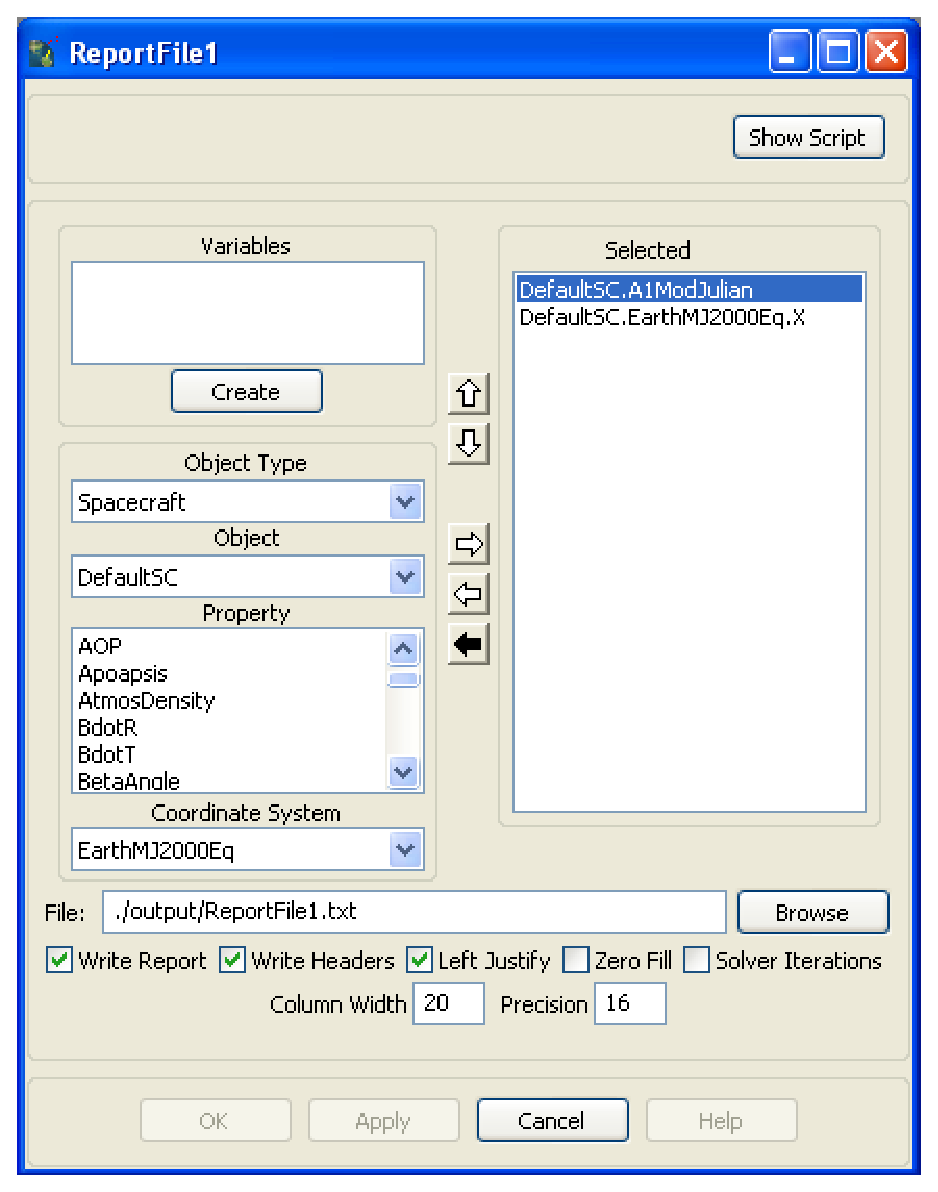
\includegraphics[scale=0.5]{Images/ParameterSubpanel.eps}
\caption{\label{figure:ParameterSubpanel}The Updated Parameter Subpanel}
\end{center}
\end{figure}

The propagator subsystem needs information about the global origin for the forces in a force model.
Figure~\ref{figure:PropPanelUpdate} shows one way to add this data to the panel.

\begin{figure}
\begin{center}
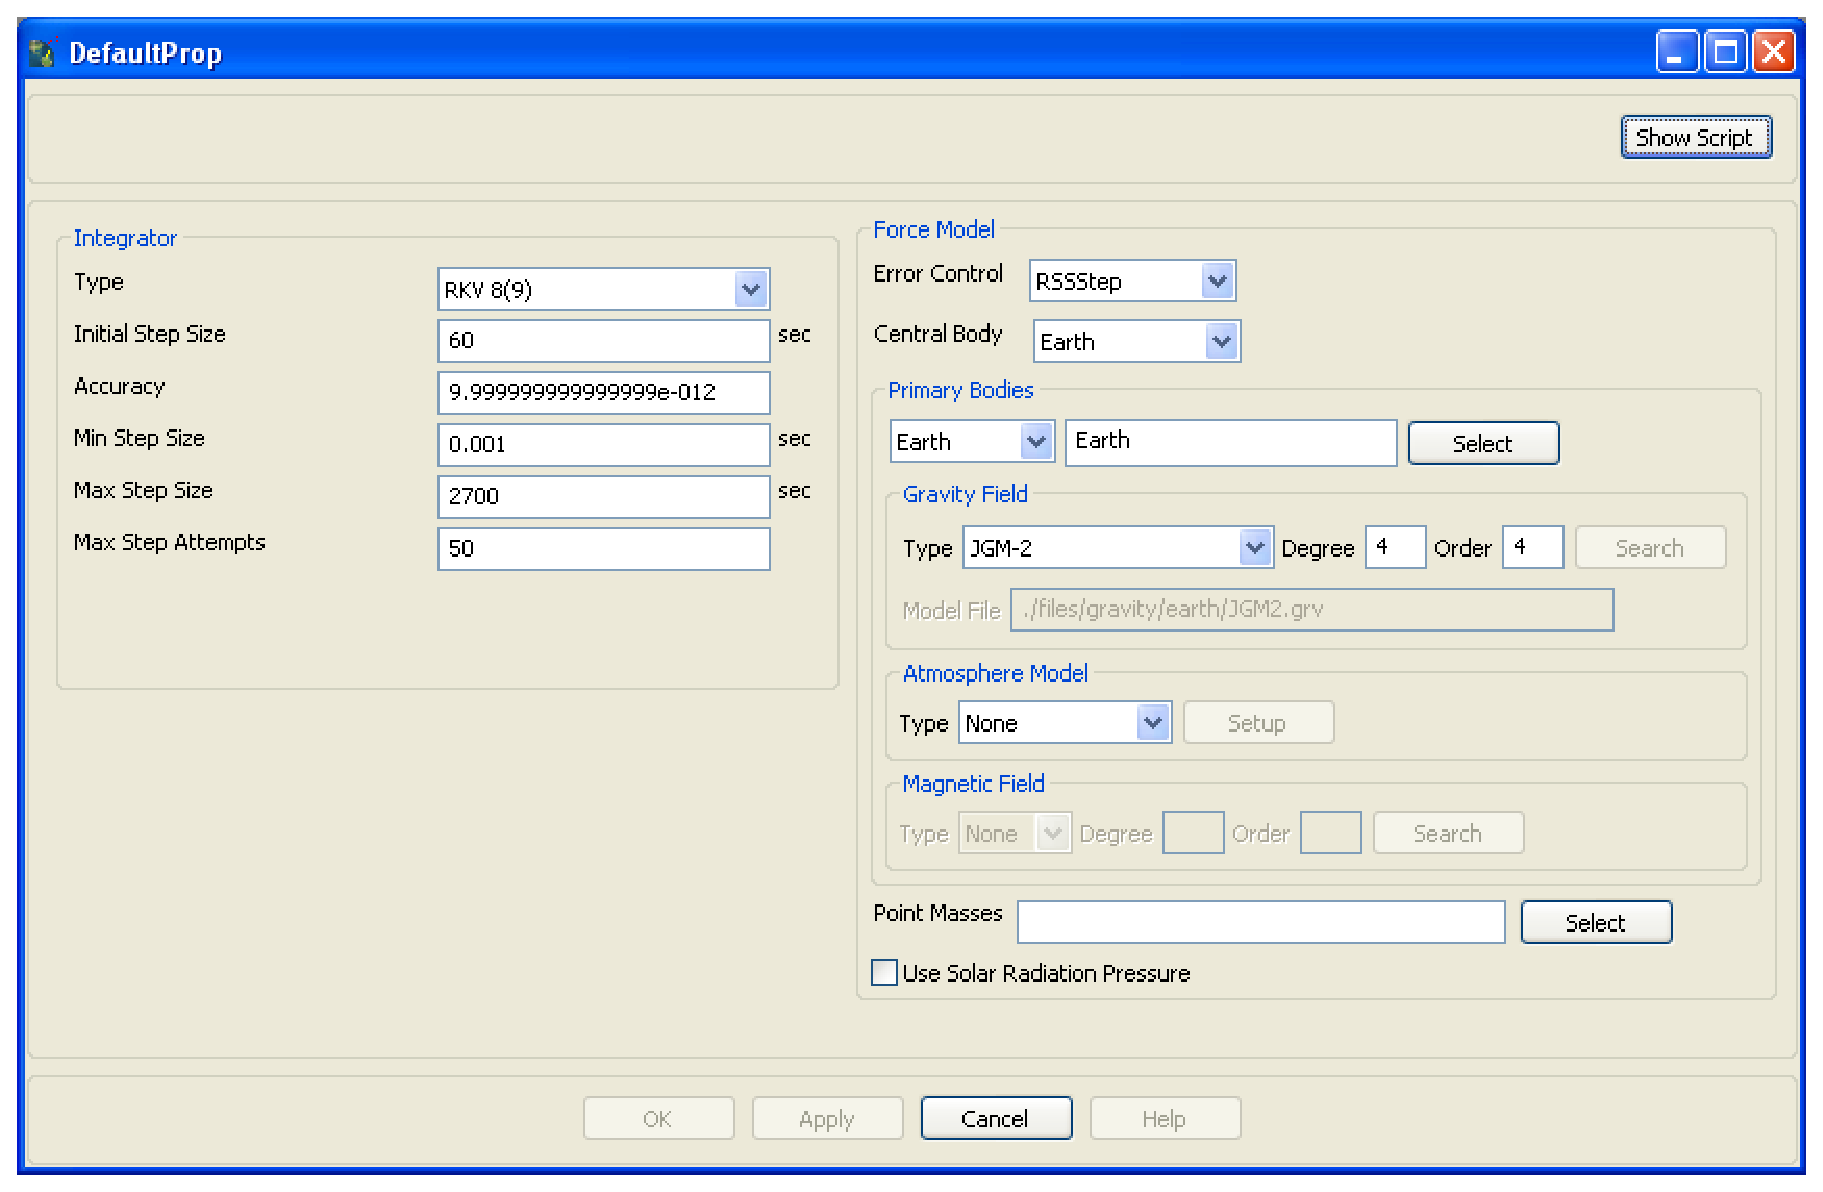
\includegraphics[scale=0.5]{Images/PropPanel.eps}
\caption{\label{figure:PropPanelUpdate}Addition of the Propagation Origin}
\end{center}
\end{figure}

The OpenGL panel needs to be updated to allow configuration of the capabilities described in Section
\ref{sub:OpenGLViewPoints}. Users can use the settings on this panel to specify both the coordinate
system used to plot the mission data and the location and orientation of the viewpoint used to
observe these data. In some cases, the viewpoint will not be a fixed point in space -- for example,
users will be able to view a spacecraft's environment in the simulation by specifying the location
and orientation of the viewpoint relative to the spacecraft in a spacecraft centered coordinate
system, and thus observe how other objects move in relation to that spacecraft.

\section{Validation}

In this section, several tables are presented that show the data for a single state in several
different coordinate systems. GMAT tests will be run that transform between these systems and
validates that the conversions are in agreement with the data in the tables to an acceptable level
of precision. The test data were generated in Astrogator by GSFC, Code 595. This output should be in
agreement with GMAT results to at least one part in $10^{12}$. (Subject to change once tests are run
-- seems like a good value as a starting point.)

\subsection{Tests for a LEO}

Table~\ref{table:LEOTests} lists the expected state data for a spacecraft orbiting near the Earth.

\begin{table}
\caption{\label{table:LEOTests}Coordinate Conversions for an orbit near the Earth}
\centerline{
%\begin{sidewaystable}
\begin{tabular}{|p{1.4in}|c|c|c|c|c|c|}
\hline
\multicolumn{7}{|c|}{\textbf{A LEO State}}\tabularnewline
\hline
\hline
\textbf{Epoch:}&
\multicolumn{2}{c|}{UTC Gregorian}&
\multicolumn{2}{c|}{UTC Julian}&
\multicolumn{2}{c|}{Ephemeris Time}\tabularnewline
\hline
\hline
&
\multicolumn{2}{c|}{1 Jan 2005 12:00:00.00}&
\multicolumn{2}{c|}{2453372}&
\multicolumn{2}{c|}{2453372.00074287}\tabularnewline
\hline
\hline
\textbf{Coordinate System}&
\textbf{X}&
\textbf{Y}&
\textbf{Z}&
$V_{x}$&
$V_{y}$&
$V_{z}$\tabularnewline
\hline
\hline
{\footnotesize Earth Centered Mean J2000 Equator}&
{\footnotesize 15999.999999999998}&
{\footnotesize 0.0000000000000}&
{\footnotesize 0.0000000000000}&
{\footnotesize 0.0000000000000}&
{\footnotesize 3.8662018270519716}&
{\footnotesize 3.8662018270519711}\tabularnewline
\hline
{\footnotesize Earth Centered Fixed}&
{\footnotesize 3100.7006422193112}&
{\footnotesize 15696.674760971226}&
{\footnotesize 7.54822029656669}&
{\footnotesize -2.6485022470204602}&
{\footnotesize 0.5213224286561129}&
{\footnotesize 3.8663431768510996}\tabularnewline
\hline
{\footnotesize Earth Centered Mean Ecliptic of Date}&
{\footnotesize 15999.988100569937}&
{\footnotesize 19.513619701949061}&
{\footnotesize 0.0163246416692983}&
{\footnotesize -0.0062037647908650}&
{\footnotesize 5.0850309969931660}&
{\footnotesize 2.0093417847447261}\tabularnewline
\hline
{\footnotesize Earth Centered Mean Ecliptic of J2000}&
{\footnotesize 15999.999999999998}&
{\footnotesize 0.0000000000000}&
{\footnotesize 0.0000000000000}&
{\footnotesize 0.0000000000000}&
{\footnotesize 5.0850575916827729}&
{\footnotesize 2.0092840576358051}\tabularnewline
\hline
{\footnotesize Earth Centered Mean of Date }&
{\footnotesize 15999.9881005699370}&
{\footnotesize 17.8969907643261870}&
{\footnotesize 7.7768465297859297}&
{\footnotesize -0.0062037647908650}&
{\footnotesize 3.8661983573941092}&
{\footnotesize 3.8662003193814876}\tabularnewline
\hline
\end{tabular}
%\end{sidewaystable}
}
\end{table}

\subsection{Tests for a Libration Point State}

Table~\ref{table:L2Tests} lists the expected state data for a spacecraft flying near the Earth-Sun.

\begin{table}
\caption{\label{table:L2Tests}Coordinate Conversions for an orbit near the Earth/Moon-Sun L2 Point}
\centerline{
%\begin{sideways}
\begin{tabular}{|p{1.25in}|c|c|c|c|c|c|}
\hline
\multicolumn{7}{|c|}{\textbf{A L2 State}}\tabularnewline
\hline
\hline
\textbf{Epoch:}&
\multicolumn{2}{c|}{UTC Gregorian}&
\multicolumn{2}{c|}{UTC Julian}&
\multicolumn{2}{c|}{Ephemeris Time}\tabularnewline
\hline
\hline
&
\multicolumn{2}{c|}{25 Sep 2003 16:22:47.94}&
\multicolumn{2}{c|}{2452908.18249931}&
\multicolumn{2}{c|}{2452908.18324218}\tabularnewline
\hline
\hline
\textbf{Coordinate System}&
\textbf{X}&
\textbf{Y}&
\textbf{Z}&
$V_{x}$&
$V_{y}$&
\textbf{$V_{z}$}\tabularnewline
\hline
\hline
{\footnotesize Earth Centered Mean J2000 Equator}&
{\footnotesize 1152413.9609139508}&
{\footnotesize 164482.90400985131}&
{\footnotesize -270853.37069837836}&
{\footnotesize -0.0237491328055502}&
{\footnotesize 0.5463496092937017}&
{\footnotesize 0.1896952705370667}\tabularnewline
\hline
{\footnotesize Sun-Earth/Moon Barycenter L1}&
{\footnotesize 2659568.8530356660}&
{\footnotesize -467.97516783879695}&
{\footnotesize -314259.10186388291}&
{\footnotesize -0.0062197634008832}&
{\footnotesize 0.3610507604664427}&
{\footnotesize -0.0425806711166933}\tabularnewline
\hline
{\footnotesize Sun-Earth L2}&
{\footnotesize -352659.29964214563}&
{\footnotesize -0.0002161438986659}&
{\footnotesize -313927.71991658572}&
{\footnotesize 0.0027515868356648}&
{\footnotesize 0.3488514802312706}&
{\footnotesize -0.0432916179713184}\tabularnewline
\hline
{\footnotesize Solar System Barycenter Mean J2000 Earth Equator}&
{\footnotesize 151524360.68432158}&
{\footnotesize 4848014.2434389694}&
{\footnotesize 1751879.7152567047}&
{\footnotesize -1.6146582474186386}&
{\footnotesize 27.776726415749529}&
{\footnotesize 11.995657174332731}\tabularnewline
\hline
\end{tabular}
%\end{sideways}
}
\end{table}

\subsection{Tests for an Earth-Trailing State}

Table~\ref{table:EarthTrailingTests} lists the expected state data for a deep space object trailing
behind the Earth.

\begin{table}
\caption{\label{table:EarthTrailingTests}Coordinate Conversions for an Earth-Trailing
state}
\centerline{
%\begin{sideways}
\begin{tabular}{|p{1.25in}|c|c|c|c|c|c|}
\hline
\multicolumn{7}{|c|}{\textbf{An Earth-Trailing State}}\tabularnewline
\hline
\hline
\textbf{Epoch:}&
\multicolumn{2}{c|}{UTC Gregorian}&
\multicolumn{2}{c|}{UTC Julian}&
\multicolumn{2}{c|}{Ephemeris Time}\tabularnewline
\hline
\hline
&
\multicolumn{2}{c|}{1 Jan 2012 00:00:00.00}&
\multicolumn{2}{c|}{2455927.5}&
\multicolumn{2}{c|}{2455927.50074287}\tabularnewline
\hline
\hline
\textbf{Coordinate System}&
\textbf{X}&
\textbf{Y}&
\textbf{Z}&
$V_{x}$&
$V_{y}$&
$V_{z}$\tabularnewline
\hline
\hline
{\footnotesize Earth Centered Mean J2000 Equator}&
{\footnotesize 18407337.2437560}&
{\footnotesize 146717552.364272}&
{\footnotesize 2436998.6080801622}&
{\footnotesize -29.85775713588113}&
{\footnotesize 3.7988731566283533}&
{\footnotesize -0.0883535323140749}\tabularnewline
\hline
{\footnotesize Earth Centered Mean Ecliptic of Date}&
{\footnotesize 18010745.506277718}&
{\footnotesize 135634904.81496251}&
{\footnotesize -56121251.238084592}&
{\footnotesize -29.8677194647804920}&
{\footnotesize 3.3629312165175098}&
{\footnotesize -1.5921471032003145}\tabularnewline
\hline
{\footnotesize Earth Centered Mean Ecliptic of J2000}&
{\footnotesize 18407337.2437560}&
{\footnotesize 135580104.86024788}&
{\footnotesize -56124988.196549937}&
{\footnotesize -29.8577571358811300}&
{\footnotesize 3.4502529604822207}&
{\footnotesize -1.5921677410083135}\tabularnewline
\hline
{\footnotesize Solar System Barycenter Mean J2000 Earth Equator}&
{\footnotesize -7095223.559007301}&
{\footnotesize 279535881.30854195}&
{\footnotesize 60015670.739229225}&
{\footnotesize -59.6890476068945470}&
{\footnotesize -0.969033406060170}&
{\footnotesize -2.1549980100429815}\tabularnewline
\hline
{\footnotesize Sun Centered Earth Equator Mean J2000}&
{\footnotesize -6610248.770514084}&
{\footnotesize 279718577.50517684}&
{\footnotesize 60095016.884433664}&
{\footnotesize -59.6964420074725410}&
{\footnotesize -0.9617072219755838}&
{\footnotesize -2.1516618821901923}\tabularnewline
\hline
{\footnotesize Venus Centered Fixed}&
{\footnotesize 234671807.87997022}&
{\footnotesize -184530264.43020287}&
{\footnotesize -49090196.384031780}&
{\footnotesize 87.7042809962516540}&
{\footnotesize 130.412316317457850}&
{\footnotesize -3.652395853117925}\tabularnewline
\hline
{\footnotesize Moon Centered Fixed}&
{\footnotesize -28218680.593746454}&
{\footnotesize -133515637.46513638}&
{\footnotesize -56782561.270103499}&
{\footnotesize -325.9434285713376800}&
{\footnotesize 70.716401043687014}&
{\footnotesize -2.3269361125638657}\tabularnewline
\hline
{\footnotesize Moon Centered Inertial Moon Equator}&
{\footnotesize 18009331.473252095}&
{\footnotesize 146686558.45310178}&
{\footnotesize 2386670.4083221816}&
{\footnotesize -29.7707871076046790}&
{\footnotesize 2.8992895961634191}&
{\footnotesize -0.4430059951218515}\tabularnewline
\hline
{\footnotesize Jupiter Centered Inertial Jupiter Equator}&
{\footnotesize -562256455.23257434}&
{\footnotesize -225513430.99244595}&
{\footnotesize -25746106.471387718}&
{\footnotesize -50.5813599808322610}&
{\footnotesize -13.854862630504574}&
{\footnotesize -0.5555336109134552}\tabularnewline
\hline
{\footnotesize Mars Centered Inertial Mars Equator}&
{\footnotesize 207783148.71266919}&
{\footnotesize -43368297.655312374}&
{\footnotesize 13161295.341311477}&
{\footnotesize -19.7427310285643220}&
{\footnotesize 35.2164929323613260}&
{\footnotesize -21.767269119097524}\tabularnewline
\hline
{\footnotesize Mars Centered Fixed}&
{\footnotesize 127577563.32704885}&
{\footnotesize -169644368.24313599}&
{\footnotesize 13138473.444519326}&
{\footnotesize -12016.3787728729480}&
{\footnotesize -9003.4840556769759}&
{\footnotesize -21.769072220711045}\tabularnewline
\hline
\end{tabular}
%\end{sideways}
}
\end{table}

\section{Some Mathematical Details}

\textbf{This section will probably appear in some form in the mathematical specifications. I'm
leaving it here until I can confirm that assumption.}

A spatial coordinate system is fully specified by defining the origin of the system and two
orthogonal directions. Given these pieces of data, space can be gridded into triplets of numbers
that uniquely identify each point. The purpose of this section is to provide some guidance into how
to proceed with the definition of the coordinate system axes once the origin and two directions are
specified.

\subsection{Defining the Coordinate Axes}

The coordinate system axes are defined from the two orthogonal directions in the system
specification. These directions are given two of the three labels $\hat{X}$, $\hat{Y}$, and
$\hat{Z}$. These labels are used to define the corresponding directions for the coordinate
system. The third axis is calculated by taking the inner product of the other two axes, using
\begin{eqnarray}
\hat{X} & = & \hat{Y}\times\hat{Z}\nonumber \\
\hat{Y} & = & \hat{Z}\times\hat{X}\nonumber \\
\hat{Z} & = & \hat{X}\times\hat{Y}\label{eq:UnitVectorTriplets}\end{eqnarray}

\subsection{Setting Directions in GMAT}

The principal directions for a coordinate system are set in GMAT by specifying a primary direction
and a secondary direction. The specified secondary axis need not be orthogonal (i.e. perpendicular)
to the primary axis. Given a primary direction $\vec{P}$ and a secondary direction $\vec{S}$, the
primary axis is oriented along a unit vector given by
\begin{equation}\hat{P}=\frac{\vec{P}}{\left|\vec{P}\right|}\end{equation}

The unit vector defining the secondary axis is constructed by projecting the secondary direction
$\vec{S}$ into the plane perpendicular to the primary direction, and unitizing the resulting vector.
This is done by calculating
\begin{equation} \hat{S}=\frac{\vec{S}-\left(\vec{S}\cdot\hat{P}\right)\hat{P}}{\left|\vec{S}
-\left(\vec{S}\cdot\hat{ P}\right)\hat{P}\right|}\end{equation}

In general, two points are needed to specify a direction.

\chapter{Calculation Objects} \label{Ch:CalculationObjects}

GMAT has the ability to calculate numerous quantities that are
dependent upon the states of objects, coordinate systems, and the
mission sequence.   These calculation objects can range from the
spacecraft state, to the local atmospheric density, to the
positions of celestial bodies with respect to spacecraft, or other
celestial bodies.  In chapter, we present how GMAT performs these
calculations by showing the mathematical algorithms.

The chapter begins by discussing different orbit state
representations.  Each of the orbit state representations
available in GMAT are defined.  Next we present the algorithms
used to convert between different state representations.  These
include the Keplerian elements, modified Keplerian elements,
Cartesian state, spherical state, and the equinoctial elements. In
the second section we present how GMAT calculates all calculation
parameters. Examples include the orbit period, percent shadow, and
energy. The algorithms to calculate all parameters are included
and described in detail. We conclude this chapter with a
presentation of the algorithms used to calculate libration point
and barycenter locations.

\section{Spacecraft State Representations} \index{Orbit state
representations}

There are several state representations that can be used in GMAT
to define the state of a spacecraft object.  These include the
Keplerian elements, Cartesian state, equinoctial elements,
spherical elements, and the modified Keplerian elements.  In the
following subsections, we discuss the definitions of these states
types, and show how GMAT converts between the different state
representations.

\subsection{Definitions}

The Keplerian elements are one of the most commonly used state
representations.  They provide a way to define the spacecraft
state in way that provides an intuitive understanding of the
motion of spacecraft in orbit.  The Keplerian elements are denoted
$a$, $e$, $i$, $\omega$, $\Omega$, and $\nu$. They are defined in
detail in Table \ref{Table:KeplerianElements} and illustrated in
Fig. \ref{fig:KeplerianElements}.  Sections \ref{Sec:Cart2Kep} and
\ref{Sec:Kep2Cart} show the algorithms that GMAT uses to convert
between the Keplerian elements and the cartesian state.
\index{Keplerian elements!definition}
%

\begin{figure*}[htb]
\index{Keplerian elements} \centerline{
\begin{picture}(100,545)
\special{psfile=Images/OrbitElements.eps hoffset= -195 voffset= 75
hscale=80
vscale=80}\makebox(-78,600){$\hat{\mathbf{x}}_I$,$\Upsilon$}
\makebox(40,610){$\hat{\mathbf{x}}_{ep}$} \makebox(10,685){$\Omega$}
\makebox(215,795){$\omega$} \makebox(-120,840){$y_I$}
\makebox(-135,968){$\mathbf{x}_p$}\makebox(-255,980){$\nu$}
\makebox(-485,1083){$z_I$} \makebox(-540,1028){$i$}
    \makebox(-610,1060){$\mathbf{h}$, $\hat{\mathbf{z}}_{ep}$}
    \makebox(-340,610){$\mathbf{N}$}
\end{picture}}\vskip -3.95 in  \caption{ The Keplerian Elements } \label{fig:KeplerianElements}
\end{figure*}

The cartesian state is another common state representation and is
often used in the numerical integration of the equations of
motion.  The cartesian state with respect to a given coordinate
system is described in detail in Table
\ref{Table:CartesianStates}. \index{Cartesian state!definition}


The equinoctial elements are a set of non-singular elements that
can be used to describe the state of a spacecraft.  Because they
are nonsingular, they are useful for expressing the equations of
motion in Variation of Parameters (VOP) form.  The elements can be
unintuitive to use however.  The equinoctial elements are
described in detail in Table \ref{Table:EquinoctialElements}.
%

\begin{figure*}[htb]
\index{Spherical elements} \centerline{
\begin{picture}(100,420)
\special{psfile=Images/SphericalElements.eps hoffset= -100 voffset=
75
hscale=55 vscale=55} \makebox(-280,360){$\mathbf{x}$}%
\makebox(140,590){$\mathbf{y}$}%
\makebox(-435,820){$\mathbf{z}$}%
\makebox(-410,530){$\lambda$}%
\makebox(-273,636){$\delta$}%
\makebox(-330,695){$\mathbf{r}$}%
\makebox(-250,770){$\mathbf{v}$}%
\makebox(90,710){$\mathbf{v}$}%
\makebox(10,675){$\hat{\mathbf{r}}$}%
\makebox(-350,650){North}%
\makebox(-275,635){$\psi$}%
\makebox(-180,597){$\alpha_f$}%
\end{picture}}\vskip -2.5 in  \caption{ The Spherical Elements } \label{fig:SphericalElements}
\end{figure*}
%

The modified Keplerian elements are similar to the Keplerian
elements except $a$ and $e$ are replaced with the radius of
periapsis $r_p$, and the radius of apoapsis $r_a$. $r_p$ and $r_a$
are often more convenient and intuitive for describing the
dimensions of a Keplerian orbit than $a$ and $e$.  The modified
Keplerian elements are defined in detail in Table
\ref{Table:ModKeplerianElements}. Note that both the Keplerian and
modified Keplerian elements are undefined for parabolic orbits
because the semimajor axis is infinite.  Currently, GMAT does not
support parabolic orbits for this reason.  Let's begin by looking
at how GMAT converts from the Cartesian state to the Keplerian
elements.

\index{Modified Keplerian elements!definition}
%

\subsection{Cartesian State to Keplerian Elements}\label{Sec:Cart2Kep}  \index{Cartesian state!to
Keplerian} \index{Keplerian elements!from cartesian}

The conversion from the Cartesian state to the Keplerian elements
has four special cases:  elliptic inclined, circular inclined,
elliptic equatorial, and circular equatorial.  Certain orbital
elements are undefined for some of the cases.  For example, the
right ascension of the ascending node, $\Omega$, is undefined for
equatorial orbits.  However, computer systems don't handle undefined
values gracefully.  In this section, we'll see how the orbital
elements are defined for each of the special cases, and how GMAT
calculates the orbital elements for each case\cite{Vallado:02}.

%
\begin{table*} \caption{The Cartesian State}
\centering \index{Cartesian state!definition}
\begin{tabular}{p{.5 in} p{2.0 in}}
  \hline\hline
  % after \\: \hline or \cline{col1-col2} \cline{col3-col4} ...
   Symbol &  Description \\
  \hline
  $x$ &  $x$-component of position\\
%
  $y$ &  $y$-component of position \\
  %
  $z$ &  $z$-component of position \\
  %
  $\dot{x}$ &  $x$-component of velocity\\
  %
  $\dot{y}$ & $y$-component of velocity\\
  %
  $\dot{z}$ & $z$-component of velocity \\
  \hline\hline \label{Table:CartesianStates}
\end{tabular}
\end{table*}

\begin{table*} \caption{The Keplerian Elements (also see Fig. \ref{fig:KeplerianElements})}
\centering \index{Keplerian elements!definition} (See Table
\ref{Table:ElementSpecialCases} for definitions of elements for near
circular and near equatorial orbits.)
\begin{tabular}{p{.5 in} p{1.5 in} p{3.5 in}}
  \hline\hline
  % after \\: \hline or \cline{col1-col2} \cline{col3-col4} ...
   Symbol & Name & Description \\
  \hline
  $a$ & semimajor axis & The semimajor contains information on the type and size of an orbit.
  If $a>0$ the orbit is elliptic.  If $a < 0$ the orbit is hyperbolic. $a = \infty$ for parabolic orbits. \\
 %
  $e$ & eccentricity & The eccentricity contains information on the shape of an orbit.  If $e = 0$, then the orbit is circular. If $0 < e < 1$ the orbit is
  elliptical.  If $e = 1$ the orbit is parabolic.  If $e > 1$ then the orbit is hyperbolic. \\
  %
  $i$ & inclination & The inclination is the angle between the $\hat{\mathbf{z}}_I$ axis and the orbit normal direction $\mathbf{h}$.  If $i \leq 90^{\circ}$ then the orbit is prograde.
  If $i > 90^{\circ}$ then the orbit is retrograde.  \\
  %
  $\omega$ & argument of periapsis & The argument of periapsis is the angle between a vector pointing at periapsis  and a vector pointing in the direction of the line of nodes. The argument of periapsis is undefined for circular orbits.\\
  %
  $\Omega$ & right ascension of  the ascending node& $\Omega$ is defined as the angle between $\hat{\mathbf{x}}_I$ and $\mathbf{N}$ measured
  counterclockwise.
    $\mathbf{N}$ is defined as the vector pointing from the center of the central body to the spacecraft, when the spacecraft crosses the bodies equatorial plane
  from the southern to the northern hemisphere.  $\Omega$ is undefined for equatorial orbits.   \\
  %
  $\nu$ & true anomaly & The true anomaly is defined as the angle between a vector pointing at periapsis and a vector pointing at the spacecraft.
  The true anomaly is undefined for circular orbits. \\
  \hline\hline \label{Table:KeplerianElements}
\end{tabular}
\end{table*}

%
\begin{table*} \caption{Keplerian Elements for Special Cases}
 \centering \index{Keplerian elements!special cases}
 \label{Table:ElementSpecialCases}
\begin{tabular}{p{1.25 in} p{1.35 in} p{3.2 in}  }
  \hline\hline
  % after \\: \hline or \cline{col1-col2} \cline{col3-col4} ...
   Orbit Type & Numerical Threshold & Description \\
  \hline \\
  %--------------
  Elliptic Inclined & $e \geq 10^{-11}$, $10^{-11} \leq i \leq \pi-10^{-11}$ & $\Omega$ is the angle between the $x$-axis and the line of nodes. $\omega$ is the angle between the line of nodes and the eccentricity vector, $\nu$ is
                                                     the angle between the eccentricity vector and the spacecraft position vector.\\
  %--------------
  Elliptic Equatorial & $e \geq 10^{-11}$, $i < 10^{-11} | i > \pi-10^{-11}$ & $\Omega = 0$, $\omega$ is the angle between the $x$-axis and the eccentricity vector, $\nu$ is
                                                     the angle between the eccentricity vector and the spacecraft position vector.\\
  %--------------
  Circular Inclined & $e < 10^{-11}$, $10^{-11} \leq i \leq \pi-10^{-11}$  & $\Omega$ is the angle between the $x$-axis and the line of nodes, $\omega = 0$, $\nu$ is
                                                     the angle between the line of nodes and the spacecraft position vector.\\
  %--------------
  Circular Equatorial & $e < 10^{-11}$, $i < 10^{-11} | i > \pi-10^{-11}$ & $\Omega = 0$, $\omega = 0$, $\nu$ is the angle between the $x$-axis and the spacecraft position vector. \\
  \hline\hline \label{Table:KeplerianElementsSpecialCases}
\end{tabular}
\end{table*}

\noindent Given:  $\mathbf{r}$, $\mathbf{v}$, and $\mu$\\

\noindent Find: $a$, $e$, $i$, $\omega$, $\Omega$, and $\nu$

We begin by calculating the specific angular momentum and its
magnitude.
%
\begin{equation}
     \mathbf{h} = \mathbf{r} \times \mathbf{v}
\end{equation}
%
\begin{equation}
     h = \|\mathbf{h} \|
\end{equation}
%
A vector pointing in the direction of the line of nodes is
%
\begin{equation}
     \mathbf{n} = [ \hspace{0.05 in} 0 \hspace{0.1 in} 0 \hspace{0.1 in} 1 \hspace{0.05
     in}]^T \times \mathbf{h}
\end{equation}
%
\begin{equation}
     n = \| n\|
\end{equation}
%
The orbit eccentricity and energy are calculated using
%
\begin{equation}
    r = \| \mathbf{r} \|
\end{equation}
%
\begin{equation}
    v = \| \mathbf{v} \|
\end{equation}
%
\begin{equation}
     \mathbf{e} = \displaystyle\frac{(v^2 - \displaystyle\frac{\mu}{r} )\mathbf{r} - (\mathbf{r}\cdot\mathbf{v}  )\mathbf{v}}{\mu}
\end{equation}
%
\begin{equation}
     e = \| \mathbf{e} \|
\end{equation}
%
\begin{equation}
     \xi = \frac{v^2}{2} - \frac{\mu}{r}
\end{equation}
%
For parabolic orbits, the semimajor axis is infinite
and the energy is zero. Here we check to see if the orbit is near
parabolic.  If $|1 - e| < 10^{-7}$ an error message is reported
and conversion is aborted.

The semimajor axis is computed using
%
\begin{equation}
     a = -\frac{\mu}{2\xi}
\end{equation}
%
Here we check to see if the conic section is nearly singular.
If $|a(1-e)| < .001 (km)$ then an error message is thrown and conversion is aborted.

If the above tests pass, then we continue and calculate the inclination.
%
\begin{equation}
     i = \cos^{-1}\left(\frac{h_z}{h}\right)
\end{equation}

There are four special cases for $\Omega$, $\omega$, and $\nu$ and
each case is treated differently.

\noindent\textit{Special Case 1:  Non-circular, Inclined Orbit  }

\noindent if $(e \geq 10^{-11})$  and $(10^{-11} \leq i \leq \pi-10^{-11})$, then
%
\begin{equation}
    \Omega = \cos^{-1}\left(\frac{n_x}{n}\right)
\end{equation}
%
Fix quadrant for $\Omega$: if $n_y < 0$, then $\Omega = 2\pi -
\Omega$
%
\begin{equation}
    \omega = \cos^{-1}\left( \frac{\mathbf{n}\cdot\mathbf{e}}{ne}\right)
\end{equation}
%
Fix quadrant for $\omega $:  if $e_z < 0$, then $\omega = 2\pi -
\omega$
%
\begin{equation}
    \nu = \cos^{-1}\left( \frac{\mathbf{e}\cdot\mathbf{r}}{er}\right)
\end{equation}
%
Fix quadrant for $\nu $:  if $\mathbf{r} \cdot \mathbf{v} < 0$, then
$\nu = 2\pi - \nu$

\noindent\textit{Special Case 2:  Non-circular, Equatorial Orbit
}

\noindent if $(e \geq 10^{-11})$  and $(i < 10^{-11}) | (i > \pi-10^{-11})$, then
%
\begin{equation}
    \Omega = 0
\end{equation}
%
\begin{equation}
     \omega = \cos^{-1}{\frac{e_x}{e}}
\end{equation}
%
Fix quadrant for $\omega $: if $e_y < 0$, then $\omega = 2\pi -
\omega$
%
\begin{equation}
    \nu = \cos^{-1}\left( \frac{\mathbf{e}\cdot\mathbf{r}}{er}\right)
\end{equation}
%
Fix quadrant for $\nu $:  if $\mathbf{r} \cdot \mathbf{v} < 0$, then
$\nu = 2\pi - \nu$
%

\noindent\textit{Special Case 3:  Circular, Inclined Orbit  }

\noindent if $(e < 10^{-11})$  and $(10^{-11} \leq i \leq \pi-10^{-11})$, then
%
\begin{equation}
    \Omega = \cos^{-1}\left(\frac{n_x}{n}\right)
\end{equation}
%
Fix quadrant for $\Omega$: if $n_y < 0$, then $\Omega = 2\pi -
\Omega$
\begin{equation}
     \omega = 0
\end{equation}
%
\begin{equation}
    \nu = \cos^{-1}\left( \frac{\mathbf{n}\cdot\mathbf{r}}{nr}\right)
\end{equation}
%
Fix quadrant for $\nu$:  if $r_z < 0$, then $\nu = 2\pi - \nu$

\noindent\textit{Special Case 4:  Circular, Equatorial Orbit  }

\noindent if $(e < 10^{-11})$  and $(i < 10^{-11}) | (i > \pi-10^{-11})$, then
%
\begin{equation}
     \Omega = 0
\end{equation}
%
\begin{equation}
     \omega = 0
\end{equation}
%
\begin{equation}
    \nu = \cos^{-1}\left( \frac{r_x}{r}\right)
\end{equation}
%
Fix quadrant for $\nu$:  if $r_y < 0$, then $\nu = 2\pi - \nu$
%

In the next section, we look at how to perform the inverse
transformation and convert from Keplerian elements to the
Cartesian state vector.

\subsection{Keplerian Elements to Cartesian \\ State}


\label{Sec:Kep2Cart} \index{Keplerian elements!to
cartesian} \index{Cartesian state!from Keplerian}

The transformation from the Keplerian elements to the Cartesian
state is one of the most common state transformations in
astrodynamics.  We previously defined both state types and refer you
to Tables \ref{Table:CartesianStates} and
\ref{Table:KeplerianElements} for their definitions.  Below we show
the algorithm that GMAT uses to convert from the Keplerian elements
to the Cartesian state\cite{Vallado:02}.

\noindent Give:  $a$, $e$, $i$, $\Omega$, $\omega$, $\nu$, and
$\mu$

\noindent Find:  $\mathbf{r}$  and $\mathbf{v}$

First check to ensure the keplerian elements are not singular. If $|a(1-e)| < .001 (km)$ then the following error message is reported and conversion is aborted: ``Warning: A nearly singular conic section was encountered while converting from the Keplerian elements to the Cartesian state.  The radius of periapsis must be greater than 1 meter."

Next check that the magnitude of the position vector is
not infinite.  If ($1+e\cos{\nu}$ $<$ 1e-30) then the following error message is reported and conversion is aborted:
``Warning: A near infinite radius  was encountered while converting from the Keplerian elements to the Cartesian state. "

Check that the orbit is not parabolic, in which case, $p$ is undefined.  If ($|1-e|< 1e-7$ then the following error message is reported and conversion is aborted:
``Warning: A nearly parabolic orbit was encountered while converting from the Keplerian elements to the Cartesian state.  The Keplerian elements are undefined for a parabolic orbit.".

Finally, define $\nu_M$ as the true anomaly placed between $-\pi$ and $\pi$.  If $e > 1$  and  $\|\nu_M\| \geq \pi - acos(1/e)$ the following error message is reported and conversion is aborted:\\
``Error: The TA value is not physically possible for a hyperbolic orbit with  the input values of SMA and ECC.\\
 The allowed values are: $-limitTA < TA < limitTA$ (degrees).
 or equivalently\\
 The allowed values are $TA < limitTA$ or $TA > 360 - limitTA$.
" where the text ``limitTA"' is replaced by the numeric value computed below in degrees:
%
\begin{equation}
    limitTA = \pi - acos(1/e)
\end{equation}
%

If the previous tests pass, we continue  by
calculating the semilatus rectum, and the radius.
%
\begin{equation}
    p = a(1-e^2);
\end{equation}
%
If $1+e\cos{\nu} < 1e-10$, then the following warning is displayed but computation proceeds. ``Warning: The orbital radius is large in  the conversion from Keplerian to Cartesian state and the state may be near a singularity causing numerical errors in the conversion."
%
\begin{equation}
     r = \frac{p}{1+e\cos{\nu}}
\end{equation}
%
The position components of the cartesian state vector are
calculated using the following three equations.
%
\begin{equation}
     x = r\left(\cos{(\omega + \nu)}\cos{\Omega} - \cos{i}\sin{(\omega + \nu)}\sin{\Omega}\right)
\end{equation}
\begin{equation}
     y = r\left(\cos{(\omega + \nu)}\sin{\Omega} + \cos{i}\sin{(\omega + \nu)}\cos{\Omega}\right)
\end{equation}
\begin{equation}
     z = r\left(\sin{(\omega + \nu)}\sin{i}\right)
\end{equation}
%

Before calculating the velocity components we check to ensure the
orbit is not parabolic.  This avoids another possible division by
zero.

\noindent if ($\| p\| < 1e-30$), then error and return: ``Warning:
GMAT does not support parabolic orbits in conversion from
keplerian to cartesian elements".

\noindent If the orbit is not parabolic, we continue and calculate
the velocity components using
%
\begin{equation}\begin{split}
     \dot{x} = \sqrt{\frac{\mu}{p}} &  \left( \cos{\nu} + e \right)
     \left( -\sin{\omega}\cos{\Omega} - \cos{i}\sin{\Omega}\cos{\omega}
     \right)- \\ &\sqrt{\frac{\mu}{p}}  \sin{\nu}\left(\cos{\omega}\cos{\Omega} - \cos{i}\sin{\Omega}\sin{\omega} \right)
      \end{split}
\end{equation}
%
\begin{equation}\begin{split}
     \dot{y} =    \sqrt{\frac{\mu}{p}}&  \left( \cos{\nu} + e \right)
     \left( -\sin{\omega}\sin{\Omega} + \cos{i}\cos{\Omega}\cos{\omega}
     \right)- \\\ & \sqrt{\frac{\mu}{p}}\sin{\nu}\left(\cos{\omega}\sin{\Omega} + \cos{i}\cos{\Omega}\sin{\omega} \right)
     \end{split}
\end{equation}
%
\begin{equation}
     \dot{z} = \sqrt{\frac{\mu}{p}} \left[ \left( \cos{\nu} + e \right)\sin{i}\cos{w} - \sin{\nu}\sin{i}\sin{\omega}      \right]
\end{equation}

Now let's look at how to calculate the cartesian state given the
equinoctial elements.

\subsection{Equinoctial Elements to Cartesian State}  \index{Equinoctial elements!to
cartesian}\index{Cartesian state!from Equinotial}
\label{Sec:EquinoctialtoCartesian}

The equinoctial elements used in GMAT are defined in Table
\ref{Table:EquinoctialElements}.  The algorithm to convert from
equinoctial elements to the cartesian state was taken from the
GTDS Mathematical Theory \cite{GTDS}.

\begin{table*} \caption{The Equinoctial Elements}
\centering \index{Equinoctial elements!definition}
\begin{tabular}{p{.5 in} p{5.0 in}}
  \hline\hline
  % after \\: \hline or \cline{col1-col2} \cline{col3-col4} ...
   Symbol &  Description \\
  \hline
  $a$ &  The semimajor contains information on the type and size of an orbit.  If $a>0$ the orbit is elliptic.  If $a < 0$ the orbit is hyperbolic. \\
%
  $h$ &  The projection of the eccentricity vector onto the $\hat{\mathbf{y}}_{ep}$ axis. \\
  %
  $k$ & The projection of the eccentricity vector onto the $\hat{\mathbf{x}}_{ep}$ axis. \\
  %
  $p$ &  The projection of $\mathbf{N}$  onto the $\hat{\mathbf{y}}_{ep}$ axis.\\
  %
  $q$ & The projection of $\mathbf{N}$  onto the $\hat{\mathbf{x}}_{ep}$ axis.  \\
  %
  $\lambda$ & The mean longitude. \\
  \hline\hline \label{Table:EquinoctialElements}
\end{tabular}
\end{table*}

\noindent Given: $a$, $h$, $k$, $p$, $q$, $\lambda$, and $\mu$

\noindent Find: $\mathbf{r}$ and $\mathbf{v}$

We begin by using the mean longitude, $\lambda$, to find the eccentric
longitude $F$.  The equation relating the two is transcendental:
\begin{equation}
     \lambda = F + h\cos{F} - k \sin{F}
\end{equation}
%
We use the Newton-Raphson method to solve for $F$, using $\lambda$
as the initial guess.  We iterate on the following equation until
$|F(i+1) - F(i)| < 10^{-10}$.
%
\begin{equation}
    F(i+1) = F(i) - \frac{f(F)}{f'(F)}
\end{equation}
%
where
%
\begin{eqnarray}
    f(F) &=& F + h \cos(F) - k\sin(F) - \lambda \\
    %
    f'(F) &=& 1 - h \sin(F) - k \cos(F)
\end{eqnarray}

Once the eccentric longitude is calculated, we continue with
%
\begin{equation}
   \beta = \frac{1}{1 + \sqrt{1 - h^2 - k^2}} \label{Eq:Beta}
\end{equation}
%
\begin{equation}
   n = \sqrt{\frac{\mu}{a^3}}
\end{equation}
%
\begin{equation}
   r = a(1 - k\cos{F} - h\sin{F})
\end{equation}

The cartesian components expressed in the equinoctial coordinate
system can be calculated using.
%
\begin{equation}
   X_1 = a\left[ ( 1 - h^2 \beta) \cos{F} + h k \beta \sin{F} - k   \right]
\end{equation}
%
\begin{equation}
   Y_1 = a\left[ ( 1 - k^2 \beta) \sin{F} + h k \beta \cos{F} - h   \right]
\end{equation}
%
\begin{equation}
  \dot{X}_1 = \frac{n a^2}{r}\left[h k \beta \cos{F} - (1 - h^2 \beta)\sin{F}   \right]
\end{equation}
%
\begin{equation}
  \dot{Y}_1 = \frac{n a^2}{r}\left[  (1 - k^2 \beta)\cos{F}  -  h k \beta \sin{F}   \right]
\end{equation}
%

The transformation from the equinoctial system to the inertial
Cartesian system is given by
%
\begin{equation}
   \mathbf{r} = X_1 \hat{\mathbf{f}} + Y_1 \hat{\mathbf{g}}
\end{equation}
%
\begin{equation}
   \mathbf{v} = \dot{X}_1 \hat{\mathbf{f}} + \dot{Y}_1 \hat{\mathbf{g}}
\end{equation}
%
where
%
\begin{equation}
    \left[ \hat{\mathbf{f}} \hspace{.1 in} \hat{\mathbf{g}} \hspace{.1 in} \hat{\mathbf{w}}
    \right]=  \frac{1}{1+p^2+q^2}\hspace{.1 in} \mathbf{Q}
\end{equation}
%
and
%
\begin{equation} \mathbf{Q} =
 \begin{pmatrix}
               1 - p^2 + q^2 &
               2 p q j &
               2 p \\
%
               2 p q&
               \left( 1 + p^2 - q^2 \right)j &
               -2 q \\
               %
               - 2 p j&
               2 q &
               \left(1 - p^2 - q^2  \right)j \\
               %
     \end{pmatrix}
\end{equation}
%
and
%
\noindent j = 1 for direct orbits ( $0\leq i \leq 90^{\circ}$ )\\
 j = -1 for retrograde orbits ( $90 < i \leq 180^{\circ}$ )\\

Currently GMAT sets $j=1$ for all input states. Now let's look at how to calculate the cartesian state given the
equinoctial elements.

\subsection{Cartesian State to Equinoctial Elements}  \index{Equinoctial elements!from cartesian}
\index{Cartesian state!to Equinotial}
\label{Sec:CartesiantoEquinoctial}

The equinoctial elements used in GMAT are defined in Table
\ref{Table:EquinoctialElements}.  The algorithm to convert from
the cartesian state to the equinoctial elements was taken from the
GTDS Mathematical Theory \cite{GTDS}.

\noindent Given:  $\mathbf{r}$, $\mathbf{v}$, and $\mu$

\noindent Find:  $a$, $h$, $k$, $p$, $q$, $\lambda$, and $\mu$

The orbit eccentricity and energy are calculated using
%
\begin{equation}
    r = \| \mathbf{r} \|
\end{equation}
%
\begin{equation}
    v = \| \mathbf{v} \|
\end{equation}
%
\begin{equation}
     \mathbf{e} = \displaystyle\frac{(v^2 - \displaystyle\frac{\mu}{r} )\mathbf{r} - (\mathbf{r}\cdot\mathbf{v}  )\mathbf{v}}{\mu}
\end{equation}
%
\begin{equation}
     e = \| \mathbf{e} \|
\end{equation}
%
\begin{equation}
     \xi = \frac{v^2}{2} - \frac{\mu}{r}
\end{equation}
%
For parabolic orbits, the semimajor axis is infinite
and the energy is zero. Here we check to see if the orbit is near
parabolic.  If $|1 - e| < 10^{-7}$ an error message is reported
and conversion is aborted.

The semimajor axis is computed using
%
\begin{equation}
     a = -\frac{\mu}{2\xi}
\end{equation}
%
Here we check to see if the conic section is nearly singular.
If $|a(1-e)| < .001 (km)$ then an error message is thrown and conversion is aborted.

The angular momentum unit vector is
%
\begin{equation}
   \hat{\mathbf{h}} = \frac{\mathbf{r} \times \mathbf{v} }{ \| \mathbf{r} \times \mathbf{v} \|}
\end{equation}
%
The unit vectors that define the equinoctial coordinate system can
be calculated using
%
\begin{equation}
   f_x = 1 - \frac{\hat{h}_x^2}{ 1 + \hat{h}_z j}
\end{equation}
%
\begin{equation}
   f_y = -\frac{\hat{h}_x \hat{h}_y}{ 1 + \hat{h}_z j}
\end{equation}
%
\begin{equation}
   f_z = -\hat{h}_x j
\end{equation}
%
where $j = 1$ if $ \hat{h}_z > 0 $  and $j = -1$ otherwise. Currently GMAT always assumes $j=1$. \\
%
\begin{equation}
    \hat{\mathbf{g}} = \hat{\mathbf{h}} \times \hat{\mathbf{f}}
\end{equation}
%

We now have the necessary information to calculate the elements
$h$, $k$, $p$, and $q$ using the following relationships.
%
\begin{equation}
    h = \mathbf{e} \cdot \hat{\mathbf{g}}
\end{equation}
%
\begin{equation}
    k = \mathbf{e} \cdot \hat{\mathbf{f}}
\end{equation}
%
\begin{equation}
    p = \frac{\hat{h}_x}{1+\hat{h}_z j}
\end{equation}
%
\begin{equation}
    q = - \frac{\hat{h}_y}{1+\hat{h}_z j}
\end{equation}
%

The final element to calculate is the mean longitude, $\lambda$.
We begin by computing the eccentric longitude, $F$,  using
%
\begin{equation}
    X_1 = \mathbf{r} \cdot \hat{\mathbf{f}}
\end{equation}
%
\begin{equation}
    Y_1 = \mathbf{r} \cdot \hat{\mathbf{g}}
\end{equation}
%
and
%
\begin{equation}
     \cos{F} = k + \frac{ \left( 1 - k^2 \beta \right) X_1 - h k \beta Y_1}{a\sqrt{1 - h^2 - k^2}}
\end{equation}
%
\begin{equation}
     \sin{F} = h + \frac{ \left( 1 - h^2 \beta \right) Y_1 - h k \beta X_1}{a\sqrt{1 - h^2 - k^2}}
\end{equation}
%
\begin{equation}
     F = \tan^{-1}_2\left( \frac{\sin{F}}{\cos{F}}\right)
\end{equation}
%
where $\beta$ is given by Eq.~\ref{Eq:Beta}.  The mean longitude
is computed using the generalized Kepler equation
%
\begin{equation}
    \lambda = F + h \cos{F} - k \sin{F}
\end{equation}

Now let's look at transformations involving the spherical
elements.

\subsection{Cartesian State to SphericalAZFPA State}
\label{Sec:CarttoSphericalAZFPA} \index{Cartesian state!to
SphericalAZFPA} \index{SphericalAZFPA! from Cartesian state }

The spherical state, with azimuth, $\alpha_f$, and flight path
angle, $\psi$, is described in Table \ref{Table:SphericalElements}
and Fig. \ref{fig:SphericalElements}.  The algorithm below shows
how GMAT converts from the cartesian state to the spherical state
with azimuth and flight path angle.

\noindent Given:  $\mathbf{r}$ and $\mathbf{v}$

\noindent Find:  $r$, $\lambda$, $\delta$, $v$, $\psi$, and
$\alpha_f$

\begin{table*} \caption{The Spherical Elements}
\centering \index{Spherical elements!definition}
\begin{tabular}{p{.5 in} p{1.5 in} p{3.5 in}}
  \hline\hline
  % after \\: \hline or \cline{col1-col2} \cline{col3-col4} ...
   Symbol & Name & Description \\
  \hline
  $r$ & $r$ & Magnitude of the position vector, $\|\mathbf{r}\|$ \\
    %
  $\lambda$ & Right Ascension & The angle between the projection of $\mathbf{r}$ into the $xy$-plane and the $x$-axis measured counterclockwise.   \\
%
  $\delta$ & Declination & The angle between $\mathbf{r}$ and the $xy$-plane. \\

  %
  $v$ & $v$ & Magnitude of the velocity vector, $\|\mathbf{v}\|$. \\
  %
  $\psi$ & Vertical flight path angle & The angle measured from a plane normal to $\mathbf{r}$ to the velocity vector $\mathbf{v}$, measured in the plane formed by $\mathbf{r}$  and $\mathbf{v}$   \\
  %
  $\alpha_f$ & Flight path azimuth & The angle measured from vector perpendicular  $\mathbf{r}$ and pointing north, to the projection of $\mathbf{v}$ into a plane normal to $\mathbf{r}$. \\
  %
    $\lambda_v$ & Right ascension of velocity &  The angle between the projection of $\mathbf{v}$ into the $xy$-plane and the $x$-axis measured counterclockwise. \\
  %
  $\delta_v$ & Declination of velocity &   The angle between the velocity vector and the $xy$-plane. \\
    \hline\hline \label{Table:SphericalElements}
\end{tabular}
\end{table*}

We begin by calculating the right ascension $\lambda$, and the
declination $\delta$.
%
\begin{equation}
    r = \| \mathbf{r} \| \label{Eq:Sphericalr}
\end{equation}
%
\begin{equation}
    \lambda= \tan^{-1}_2(y,x) \label{Eq:Sphericallambda}
\end{equation}
%
\begin{equation}
    \delta = \sin^{-1}(\frac{z}{r}) \label{Eq:Sphericaldelta}
\end{equation}
%
The magnitude of the velocity vector is simply
%
\begin{equation}
    v = \| \mathbf{v} \|  \label{Eq:Sphericalv}
\end{equation}
%
We calculate the vertical flight path angle, $psi$, using
%
\begin{equation}
    \psi = \cos^{-1}\left(  \frac{\mathbf{r} \cdot \mathbf{v} }{r v} \right)
\end{equation}
%
To calculate the azimuth angle, $\alpha_z$, we begin by
calculating the rotation matrix from the frame in which the
cartesian state is expressed in, $\mathcal{F}_{i}$, to a local
frame, $\mathcal{F}_{\ell}$, where $\hat{\mathbf{z}}$ is a unit
vector that points north.  The basis vectors of
$\mathcal{F}_{\ell}$ expressed in $\mathcal{F}_{i}$ can be
calculated using
%
\begin{equation}
    \hat{\mathbf{x}} =
    \begin{pmatrix}
        \cos(\delta)\cos(\lambda)\\
         \cos(\delta)\sin(\lambda)\\
          \sin(\delta)
    \end{pmatrix} \label{Eq:SphericalAZFPAx}
\end{equation}
%
\begin{equation}
    \hat{\mathbf{y}} =
    \begin{pmatrix}
          \cos(\lambda + \pi/2)\\
          \sin(\lambda + \pi/2)\\
          0
    \end{pmatrix}  \label{Eq:SphericalAZFPAy}
\end{equation}
%
\begin{equation}
    \hat{\mathbf{z}} =
    \begin{pmatrix}
          -\sin(\delta)\cos(\lambda)\\
          -\sin(\delta)\sin(\lambda)\\
          \cos(\delta)
    \end{pmatrix}  \label{Eq:SphericalAZFPAz}
\end{equation}
%
We can write the tranformation matrix that goes from
$\mathcal{F}_{i}$ to $\mathcal{F}_{\ell}$, $\mathbf{R}_{\ell i}$,
as
%
\begin{equation}
    \mathbf{R}_{\ell i} = [\hspace{.05 in} \hat{\mathbf{x}} \hspace{.1 in}
    \hat{\mathbf{y}} \hspace{.1in} \hat{\mathbf{z}} \hspace{.05 in}]^T
\end{equation}
%
The velocity in the local frame,  $\mathbf{v}'$, can be written as
%
\begin{equation}
    \mathbf{v}' = \mathbf{R}_{\ell i}\mathbf{v}
\end{equation}
%
Finally, we calculate the azimuth angle using
\begin{equation}
     \alpha_f = \tan^{-1}_2( v'_y, v'_z )
\end{equation}

Now that we have looked at how to convert from the Cartesian state
to the spherical state, let's look at the inverse transformation
that converts from the spherical state (with $\psi$ and
$\alpha_f$) to the cartesian state.

\subsection{SphericalAZFPA State to Cartesian State} \index{Cartesian
state!from SphericalAZFPA} \index{SphericalAZFPA! to Cartesian
state } \label{Sec:SphericalAZFPAtoCartesian}

In this section we present the algorithm used to convert from the
spherical state (with $\psi$ and $\alpha_f$) to the cartesian
state.

\noindent Given: $r$, $\lambda$, $\delta$, $v$, $\psi$, and
$\alpha_f$

\noindent Find:  $\mathbf{r}$ and $\mathbf{v}$

The components of the position vector are calculated using
%
\begin{eqnarray}
     x &=& r\cos{\delta} \cos{ \lambda } \label{Eq:Sphericalx}\\
     %
     y &=& r\cos{\delta}\sin{\lambda}  \label{Eq:Sphericaly}\\
     %
     z &=& r\sin{\delta} \label{Eq:Sphericalz}
\end{eqnarray}
%

We can write the velocity vector in terms of $v$, $\psi$, and
$\alpha_f$ as,
%
\begin{equation}
     \mathbf{v} = v\left[\cos( \psi )\hat{\mathbf{x}} + \sin( \psi )\sin(\alpha_f)\hat{\mathbf{y}} +
     \sin( \psi )\cos(\alpha_f)\hat{\mathbf{z}}\right]
     \label{Eq:SphericalAZFPAv}
\end{equation}
%
where, $\hat{\mathbf{x}}$, $\hat{\mathbf{y}}$, and
$\hat{\mathbf{x}}$ are given in Eqs.~(\ref{Eq:SphericalAZFPAx}),
(\ref{Eq:SphericalAZFPAy}), and (\ref{Eq:SphericalAZFPAz})
respectively.  Breaking down Eq.~(\ref{Eq:SphericalAZFPAv}) into
components gives us
%
\begin{equation}
\begin{split}
      v_x = v[ \cos{\psi}\cos{\delta}\cos{\lambda}- &\sin{\psi}(\sin{\alpha_f}\sin{\lambda}
       \\
      +  &\cos{\alpha_f}\sin{\delta}\cos{\lambda})]
\end{split}
\end{equation}
%
\begin{equation}
\begin{split}
      v_y = v[
      \cos{\psi}\cos{\delta}\sin{\lambda}+&\sin{\psi}(\sin{\alpha_f}\cos{\lambda}
      \\
      -&\cos{\alpha_f}\sin{\delta}\sin{\lambda})]
\end{split}
\end{equation}
%
\begin{equation}
      v_z = v[\cos{\psi}\sin{\delta}+\sin{\psi}\cos{\alpha_f}cos{\delta}]
\end{equation}
%

\subsection{Cartesian State to SphericalRADEC State}\index{Cartesian state! to
SphericalRADEC} \index{SphericalRADEC! from Cartesian State }

The conversion form the Cartesian state to the spherical state
with right ascension of velocity, $\lambda_v$, and declination of
velocity, $\delta_v$, is very similar to the transformation shown
in Sec. \ref{Sec:CarttoSphericalAZFPA}.  The algorithm to
calculate $\lambda_v$ and $\delta_v$ is shown below.

\noindent Given:  $\mathbf{r}$ and $\mathbf{v}$

\noindent Find:  $r$, $\lambda$, $\delta$, $v$, $\lambda_v$, and
$\delta_v$

To calculate $r$, $\lambda$, $\delta$, and $v$ we use
Eqs.~(\ref{Eq:Sphericalr}), (\ref{Eq:Sphericallambda}),
(\ref{Eq:Sphericaldelta}), and (\ref{Eq:Sphericalv}) respectively.
The right ascension of velocity, $\lambda_v$, and declination of
velocity, $\delta_v$, are calculated using
%
\begin{equation}
    \lambda_v= \tan^{-1}_2(v_y,v_x) \label{Eq:Sphericallambdav}
\end{equation}
%
\begin{equation}
    \delta_v = \sin^{-1}(\frac{v_z}{v}) \label{Eq:Sphericaldeltav}
\end{equation}
%

In the next section, we show the the transformation from the
spherical state  with right ascension of velocity, $\lambda_v$,
and declination of velocity, $\delta_v$, to the cartesian state.

\subsection{SphericalRADEC State to Cartesian State} \index{Cartesian state!from SphericalRADEC }

This transformation is similar to the conversion presented in Sec
\ref{Sec:SphericalAZFPAtoCartesian}.  The primary difference is
how the velocity is represented.

\noindent Given:  $r$, $\lambda$, $\delta$, $v$, $\lambda_v$, and
$\delta_v$

\noindent Find:  $\mathbf{r}$ and $\mathbf{v}$

The position components are calculated using Eqs.
(\ref{Eq:Sphericalx}), (\ref{Eq:Sphericaly}), and
(\ref{Eq:Sphericalz}).  The velocity components are calculated
using
%
\begin{eqnarray}
    v_x &=& v\cos{\lambda_v}\cos{\delta_v}\\
    v_y &=& v_x\tan{\lambda_v}\\
    v_z &=& v\sin{\delta_v}
\end{eqnarray}

In the last few subsections, we have looked at transformations
involving the spherical elements.  Now let's look at
transformations involving the modified Keplerian elements.

\subsection{Keplerian or Cartesian, to Modified Keplerian Elements} \index{Modified Keplerian elements!from Keplerian} \index{Keplerian elements!to modified Keplerian}

The modified Keplerian elements, described in Table
\ref{Table:ModKeplerianElements}, are similar to the classical
Keplerian elements.  The modified Keplerian elements use the
radius of apoapsis, $r_a$, and the radius of periapsis, $r_p$, to
describe the size and shape of an orbit.  The remaining elements,
$i$, $\Omega$, $\omega$, and $\nu$, are the same for both the
Keplerian and modified Keplerian elements. The modified Keplerian
elements, like the Keplerian elements, are undefined for parabolic
orbits.  Let's look at how GMAT calculates the modified


\begin{table*} \caption{The Modified Keplerian Elements}
\centering\index{Modified Keplerian elements!definition}
\begin{tabular}{p{.5 in} p{1.5 in} p{3.5 in}}
  \hline\hline
  % after \\: \hline or \cline{col1-col2} \cline{col3-col4} ...
   Symbol & Name & Description \\
  \hline
  $r_p$ & radius of periapsis & The radius of periapsis is the radius at the spacecrafts closest approach to the central body.  The radius of periapsis must be greater than zero, parabolic orbits are not currently supported. \\
%
  $r_a$ & radius of apoapsis  &  For an elliptic orbit $r_a$ is the radius at the spacecrafts farthest distance from the central body and $r_a>r_p$.  For hyperbolic orbits, $r_a<r_p$ and $r_a < 0 $  \\
  %
  $i$ & inclination & The inclination is the angle between the $\hat{\mathbf{z}}_I$ axis and the orbit normal direction $\mathbf{h}$.  If $i \leq 90^{\circ}$ then the orbit is prograde.
  If $i > 90^{\circ}$ then the orbit is retrograde.  \\
  %
  $\omega$ & argument of periapsis & The argument of periapsis is the angle between a vector pointing at periapsis,
  $\mathbf{x}_p$, and a vector pointing at the spacecraft. The argument of periapsis is undefined for circular orbits.\\
  %
  $\Omega$ & right ascension of  the ascending node& $\Omega$ is defined as the angle between $\hat{\mathbf{x}}_I$ and $\mathbf{N}$ measured
  counterclockwise.
    $\mathbf{N}$ is defined as the vector pointing from the center of the central body to the spacecraft, when the spacecraft crosses the bodies equatorial plane
  from the southern to the northern hemisphere.  $\Omega$ is undefined for equatorial orbits.   \\
  %
  $\nu$ & true anomaly & The true anomaly is defined as the angle between a vector pointing at periapsis, $\mathbf{x}_p$, and a vector pointing at the spacecraft.
  The true anomaly is undefined for circular orbits. \\
  \hline\hline \label{Table:ModKeplerianElements}
\end{tabular}
\end{table*}


\noindent Given:  $a$, $e$, $i$, $\omega$, $\Omega$, and $\nu$, or
$\mathbf{r}$, $\mathbf{v}$, and $\mu$

\noindent Find:  $r_p$ and $r_a$

If we are given the Cartesian state, we first calculate the
orbital elements using the algorithm in Sec. \ref{Sec:Kep2Cart}.
Knowing the Keplerian elements, we calculate $r_a$ and $r_p$ using
%
\begin{equation}
     r_a = a(1+e)
\end{equation}
%
\begin{equation}
     r_p = a(1-e)
\end{equation}

Now let's look at the inverse transformation.

\subsection{Modified Keplerian Elements to Keplerian Elements} \index{Modified
Keplerian elements!to Keplerian}   \index{Keplerian elements!from
modified Keplerian}

The conversion from modified Keplerian elements to the Keplerian
elements is discussed below.  To perform the conversion, we use
relationships that allow us to write the semimajor axis, $a$, and
the eccentricity, $e$, in terms of $r_a$ and $r_p$.

\noindent Given:  $r_p$, $r_a$, $i$, $\omega$, $\Omega$, and $\nu$

\noindent Find:  $a$ and $e$

We begin by calculating the eccentricity using
%
\begin{equation}
    e = \frac{1 - \displaystyle\frac{r_p}{r_a}}{1 + \displaystyle\frac{r_p}{r_a}}
\end{equation}
%
The semimajor axis is calculated using
%
\begin{equation}
    a = \displaystyle\frac{r_p}{1 - e}
\end{equation}

This concludes our discussion of state transformations. In the
last few subsections we presented the algorithms used to convert
between different orbit state representations used in GMAT.  These
include the Cartesian state, the Keplerian elements, the modified
Keplerian elements, and two spherical state parameterizations.  In
the next section, we present the algorithms used to calculate
 properties such as orbit period, beta angle, and mean motion to
 name a few.

\section{Simple Parameters}

Simple parameters, which we will abbreviate as simply ``parameters",
are properties of spacecraft or other objects that are only
dependent upon one of the following:  CoordinateSystem, CentralBody,
or None.  An example of a simple parameter is the magnitude of a
spacecrafts velocity vector.  The spacecrafts velocity vector is
dependent upon the coordinate system in which it is expressed.  Once
we have specified a coordinate system, it is trivial to calculate
the velocity vector, and therefore its magnitude, in that coordinate
system.

In GMAT, the syntax to specify a simple parameter is

\st{ObjectName.Dependency.ParameterName}

\noindent So, to calculate the magnitude of the velocity, of a
spacecraft named \st{Sat}, in the Earth Fixed frame, we would use

\st{Sat.EarthFixed.VMAG}

\noindent GMAT has the ability to calculate many parameters in
addition to \st{VMAG}.  In the following subsections, we present the
algorithms used to calculate all parameters in GMAT.  We begin each
subsection with a description of the parameter, and then give the
type of dependency.

\subsection{A1Gregorian} \index{A1Gregorian}

\noindent \textit{Description}: \st{A1Gregorian} is the epoch of an
object, in the A1 time system, given in the Gregorian date format.

\noindent \textit{Dependency}:  None.

The A1 date, in modified Julian date format is the current
independent variable for time in GMAT.  Therefore, it is not
necessary to convert the date to another system for this parameter.
The only calculation  required for this parameter is to use the
algorithm in Sec. \ref{Sec:GregorianData} to convert from Modified
Julian date format to Gregorian date format.

\subsection{A1ModJulian} \index{A1ModJulian}

\noindent \textit{Description}: \st{A1ModJulian} is the epoch of an
object, in the A1 time system, given in the modified Julian date
format.

\noindent \textit{Dependency}:  None.

The A1 date, in modified Julian date format is the current
independent variable for time in GMAT.  There are no calculations
required for this parameter.

\subsection{Altitude} \index{Altitude}

\noindent \textit{Description}: \st{Altitude} is the distance
between a spacecraft and a plane tangent to the surface of the body
at the sub-satellite point.  GMAT assumes the body is an ellipsoid.
The equatorial radius, and properties of the ellipsoid depend upon
the particular body chosen by the user.

\noindent \textit{Dependency}:  Central Body.

\noindent Given:  $\mathbf{r}$ in $\mathcal{F}_1$

\noindent Find:  $A$

\noindent Definitions:
\begin{itemize}
     %
     \item $\mathcal{F}_1$ is the coordinate system in which GMAT originally knows $\mathbf{r}$
     %
     \item $\mathcal{F}_F$ is body fixed system of the central body selected by the user.
     %
     \item $f$ is the bodies flattening coefficient
     %
     \item $R$ is the bodies mean equatorial radius
     %
    % \item $\phi_{gc}$ is the geocentric latitude of the spacecraft
     %in the body fixed frame.
     %
     \item $\phi_{gd}$ is the geodedic latitude of the spacecraft
     in the body fixed frame.
     %
     \item $h$ is the \st{Altitude} parameter
     %
\end{itemize}

First we calculate $\phi_{gd}$ using the algorithm in Sec.
\ref{Sec:Latitude}.  However, to calculate $h$, GMAT does not
convert to degrees, or use the modulo function.

Then, with $\mathbf{r}$ expressed in $\mathcal{F}_F$, we perform
%
\begin{equation}
     r_{xy} = \sqrt{ x^2 + y^2 }
\end{equation}
%
\begin{equation}
    e^2 = 2f-f^2
\end{equation}
%
\begin{equation}
            h =   \frac{ r_{xy}}{ \cos(\phi_{gd})} - \frac{R} { \sqrt{ 1 - e^2  \sin^{2}{ \phi_{gd} } } };
\end{equation}

\subsection{AOP} \index{AOP}

\noindent \textit{Description}: \st{AOP} is the argument of
periapsis of a spacecraft.  The argument of periapsis is the angle
between the eccentricity vector and a vector in the direction of the
right ascension of the ascending node.  See below for treatment of
circular and equatorial orbits.  This algorithm is adopted from
Vallado\cite{vallado2}.

\noindent \textit{Dependency}:  Coordinate System.

\noindent Given:  $\mathbf{r}$ and $\mathbf{v}$

\noindent Find:  $\omega$
\[
r = \| \mathbf{r} \|
\]
%
\[
v = \| \mathbf{v} \|
\]
%
\[
    \mathbf{e} = \displaystyle\frac{\left( v^2 - \displaystyle\frac{\mu}{r}  \right)\mathbf{r} - (\mathbf{r} \cdot \mathbf{v})\mathbf{v}}{\mu}
\]
%
\[
   e = \| \mathbf{e} \|
\]
%
\textit{Special Case:   Circular Orbit}\\
if $ e < 10^{-11}$  then, $\omega = 0.0$ and return.


\noindent Otherwise continue,
%
\[ \mathbf{h} = \mathbf{r} \times \mathbf{v} \]
%
\[ h = \| \mathbf{h} \| \]
%
\[ i = \cos^{-1}{\left(\frac{h_z}{h}  \right)}\]

\noindent \textit{Special Case:  Elliptic, Equatorial Orbit}\\
if $ i < 10^{-11}$ then,
%
\begin{equation}
    \omega = \cos^{-1}\left(\frac{e_x}{e}  \right)
\end{equation}
%
where $e_x$ is the first component of the eccentricity vector.\\
Fix quadrant for $\omega $: if $e_y < 0$, then $\omega = 2\pi -
\omega$

\noindent Otherwise continue

\noindent \textit{Special Case:  Elliptic, Inclined Orbit}\\
%
\[ \mathbf{n} = [\hspace{.05 in}0 \hspace{.1 in} 0 \hspace{.1 in} 1 \hspace{.05 in}]^T \times \mathbf{h} \]
%
\[ \omega = \cos^{-1}\frac{\mathbf{n}\cdot \mathbf{e}}{\| \mathbf{n}\|\|
\mathbf{e}\|}\]
%
Fix quadrant for $\omega $: if $e_z < 0$, then $\omega = 2\pi -
\omega$. \\Finally, $\omega$ is converted to degrees.
%
\subsection{Apoapsis} \index{Apoapsis}

\noindent \textit{Description}: \st{Apoapsis} is the parameter used
in stopping conditions to allow the stopping condition algorithm to
locate the time when a spacecraft is at apoapsis. Apoapsis is
defined as a point, along an orbital path, when the component of
velocity, in the spacecraft position vector direction, changes from
positive to negative.  The \st{Apoapsis} parameter is defined as the
dot product of the position and velocity vectors.

\noindent \textit{Dependency}:  Central Body.

\noindent Given:  $\mathbf{r}$, $\mathbf{v}$ in $\mathcal{F}_1$

\noindent Find:  $A$

\noindent Definitions:
%
\begin{itemize}
     %
     \item $\mathcal{F}_1$ is the coordinate system in which GMAT originally knows $\mathbf{r}$ and $\mathbf{v}$
     %
     \item $\mathcal{F}_2$ is a system with the MJ2000Eq axes, centered at the central body selected by the user.
     %
     \item $A$ is the \st{Apoapsis} parameter
     %
\end{itemize}
%

if ($\mathcal{F}_1 \neq \mathcal{F}_2)$ convert $\mathbf{r}$ and
$\mathbf{v}$ to $\mathcal{F}_2$.  Then,
%
\begin{equation}
     A = \mathbf{r} \cdot \mathbf{v}
\end{equation}

\subsection{AZI} \index{AZI}

\noindent \textit{Description}: \st{AZI} is the azimuth angle of a
spacecraft, as shown in Fig. \ref{fig:KeplerianElements} using the
symbol $\alpha_f$.

\noindent \textit{Dependency}:  Coordinate System.

\noindent Given:  $\mathbf{r}$, $\mathbf{v}$ and $\mathcal{F}$

\noindent Find:  $\alpha_f$


AZI is calculated using the algorithm shown in Sec.
\ref{Sec:CarttoSphericalAZFPA}.  There is little benefit using a
routine that calculates only $\alpha_f$ and not $\psi$.

\subsection{BdotT and BdotR} \index{BdotT} \index{BdotR}

\noindent \textit{Description}: The ``B" vector, $\mathbf{B}$, is
only defined for hyperbolic orbits and is the vector from the center
of mass of the central body, to the incoming hyperoblic asysmptote,
such that the length of $\mathbf{B}$ is a minimum. Another way to
say this is that $\mathbf{B}$ is perpendicular to the incoming
asymptote.   Let's define $\mathbf{S}$ as a unit vector in the
direction of the incoming asymptote.  Then, $\mathbf{T}$ is a unit
vector perpendicular to $\mathbf{S}$, that lies in the $xy$-plane of
the coordinate system, $\mathcal{F}_B$, chosen by the user.
$\mathbf{R}$ is a unit vector perpendicular to both $\mathbf{S}$ and
$\mathbf{T}$. Finally, \st{BdotT} is the dot product of $\mathbf{B}$
and $\mathbf{T}$, and \st{BdotR} is the dot product of $\mathbf{B}$
and $\mathbf{R}$. The method below was adopted from work by
Kizner\cite{Kizner:59}.

\noindent \textit{Dependency}:  Coordinate System.

\noindent Given:  $\mathbf{r}$, $\mathbf{v}$, and definition of
$\mathcal{F}_B$

\noindent Find:  $B_R$ and $B_T$

\noindent Definitions:
\begin{itemize}
     %
     \item $\mathcal{F}_1$ is the coordinate system in which GMAT originally knows
     $\mathbf{r}$ and $\mathbf{v}$
     %
     \item $\mathcal{F}_B$ is the coordinate system in which to perform B-plane
     calculations.  GMAT will place $\mathbf{T}$ in the $xy$-plane
     of  $\mathcal{F}_B$.  $\mathcal{F}_B$ must have a gravitational
     body at its origin.
     %
     \item $\mu$ is the gravitational parameter of the central body
     at the origin of $\mathcal{F}_B$
     %
     \item $B_R$ is the dot product of $\mathbf{B}$ and
     $\mathbf{R}$
     %
     \item $B_T$ is the dot product of $\mathbf{B}$ and
     $\mathbf{T}$
\end{itemize}



if the selected coordinate system does not have a celestial body as
its origin, then exit and throw an error message.\\
%
\begin{figure}[htb]
    \begin{picture}(100,200)(55,340)
        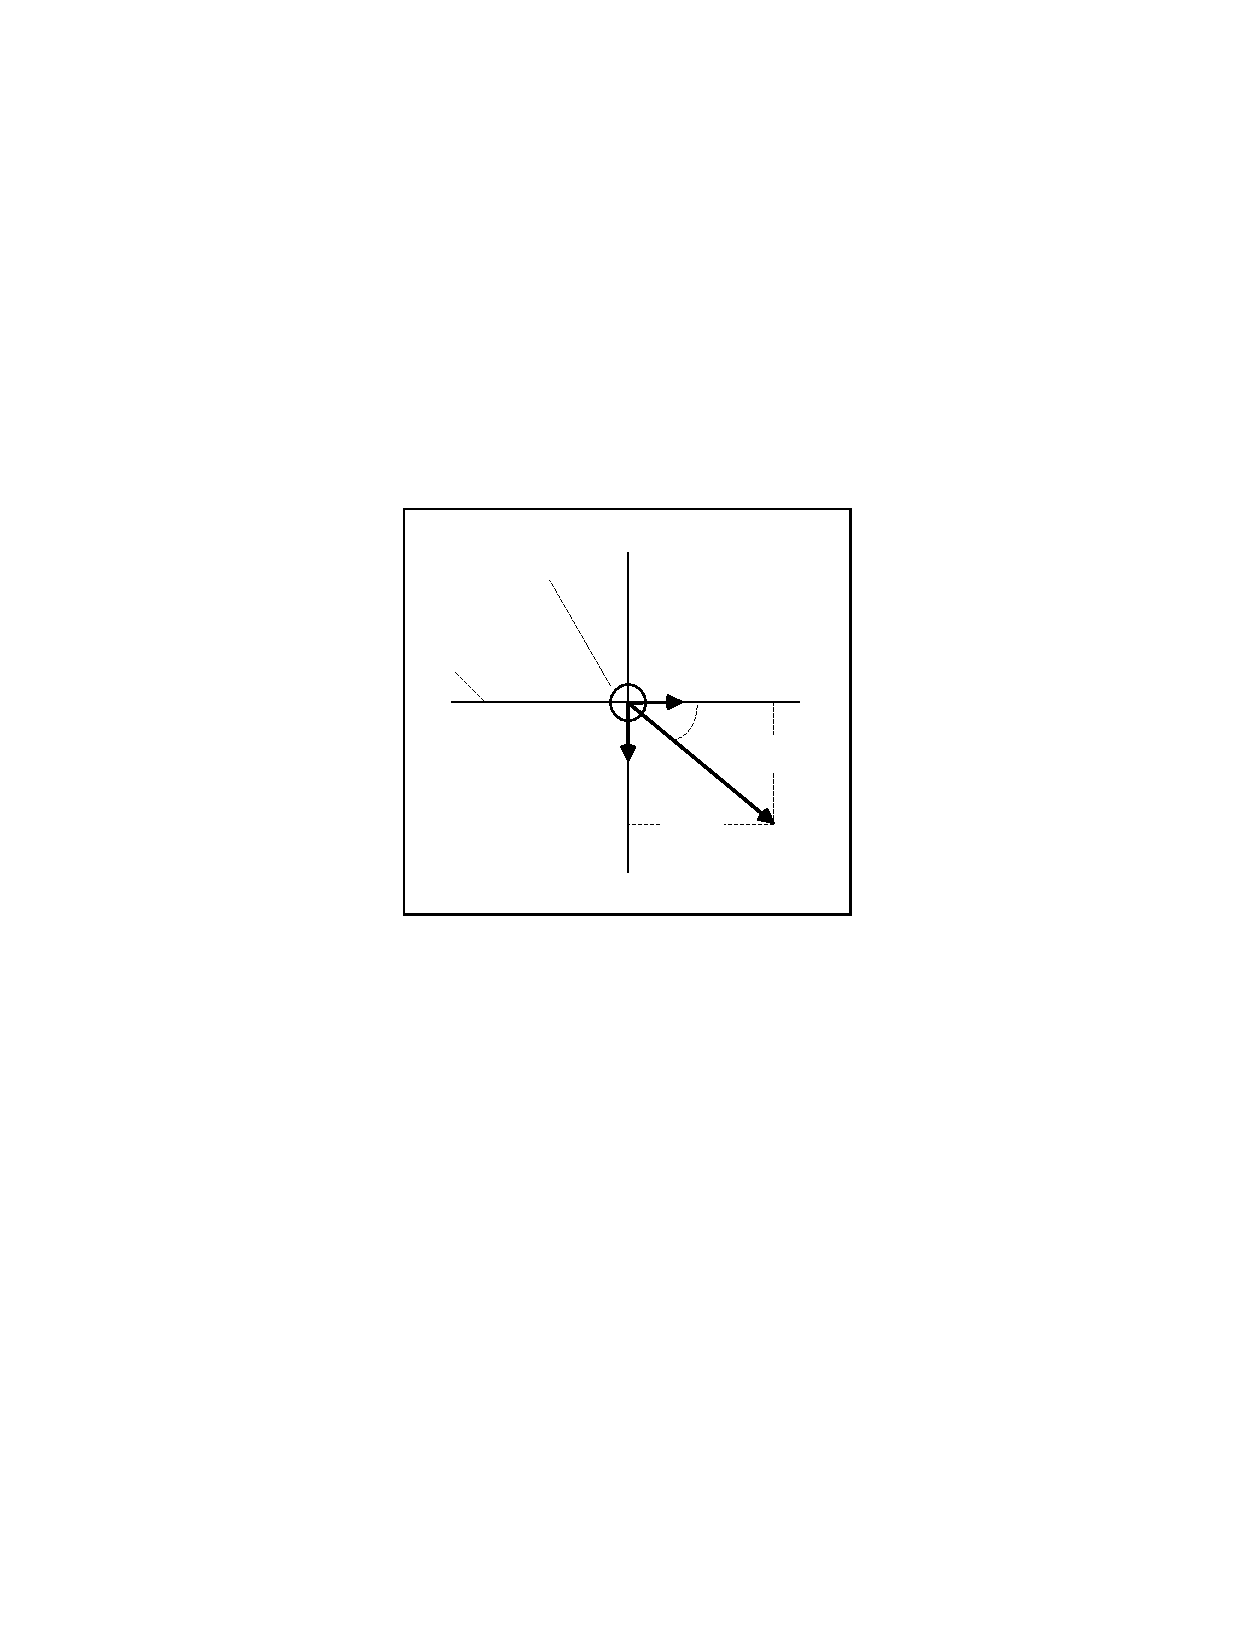
\includegraphics[scale=1]{Images/BPlaneGeometry1.eps}
    \makebox(-520,845){$\theta_B$}
    \makebox(-615,820){$\mathbf{R}$}
    \makebox(-500,810){$\mathbf{B}$}
    \makebox(-560,890){$\mathbf{T}$}
    \makebox(-760,920){$xy$-plane of $\mathcal{F}_B$ }
    \makebox(-720,990){Central Body}
    \makebox(-570,1030){$z$-axis of $\mathcal{F}_B$}
    \makebox(-580,760){$\mathbf{B}\cdot\mathbf{T}$}
    \makebox(-485,830){$\mathbf{B}\cdot\mathbf{R}$}
    \end{picture}
    \caption{Geometry of the B-Plane as Seen From a Viewpoint Perpendicular to the B-Plane}
    \label{fig:BPlaneGeometry1}
\end{figure}
%
\begin{figure}[htb]
    \begin{picture}(100,240)(125,340)
        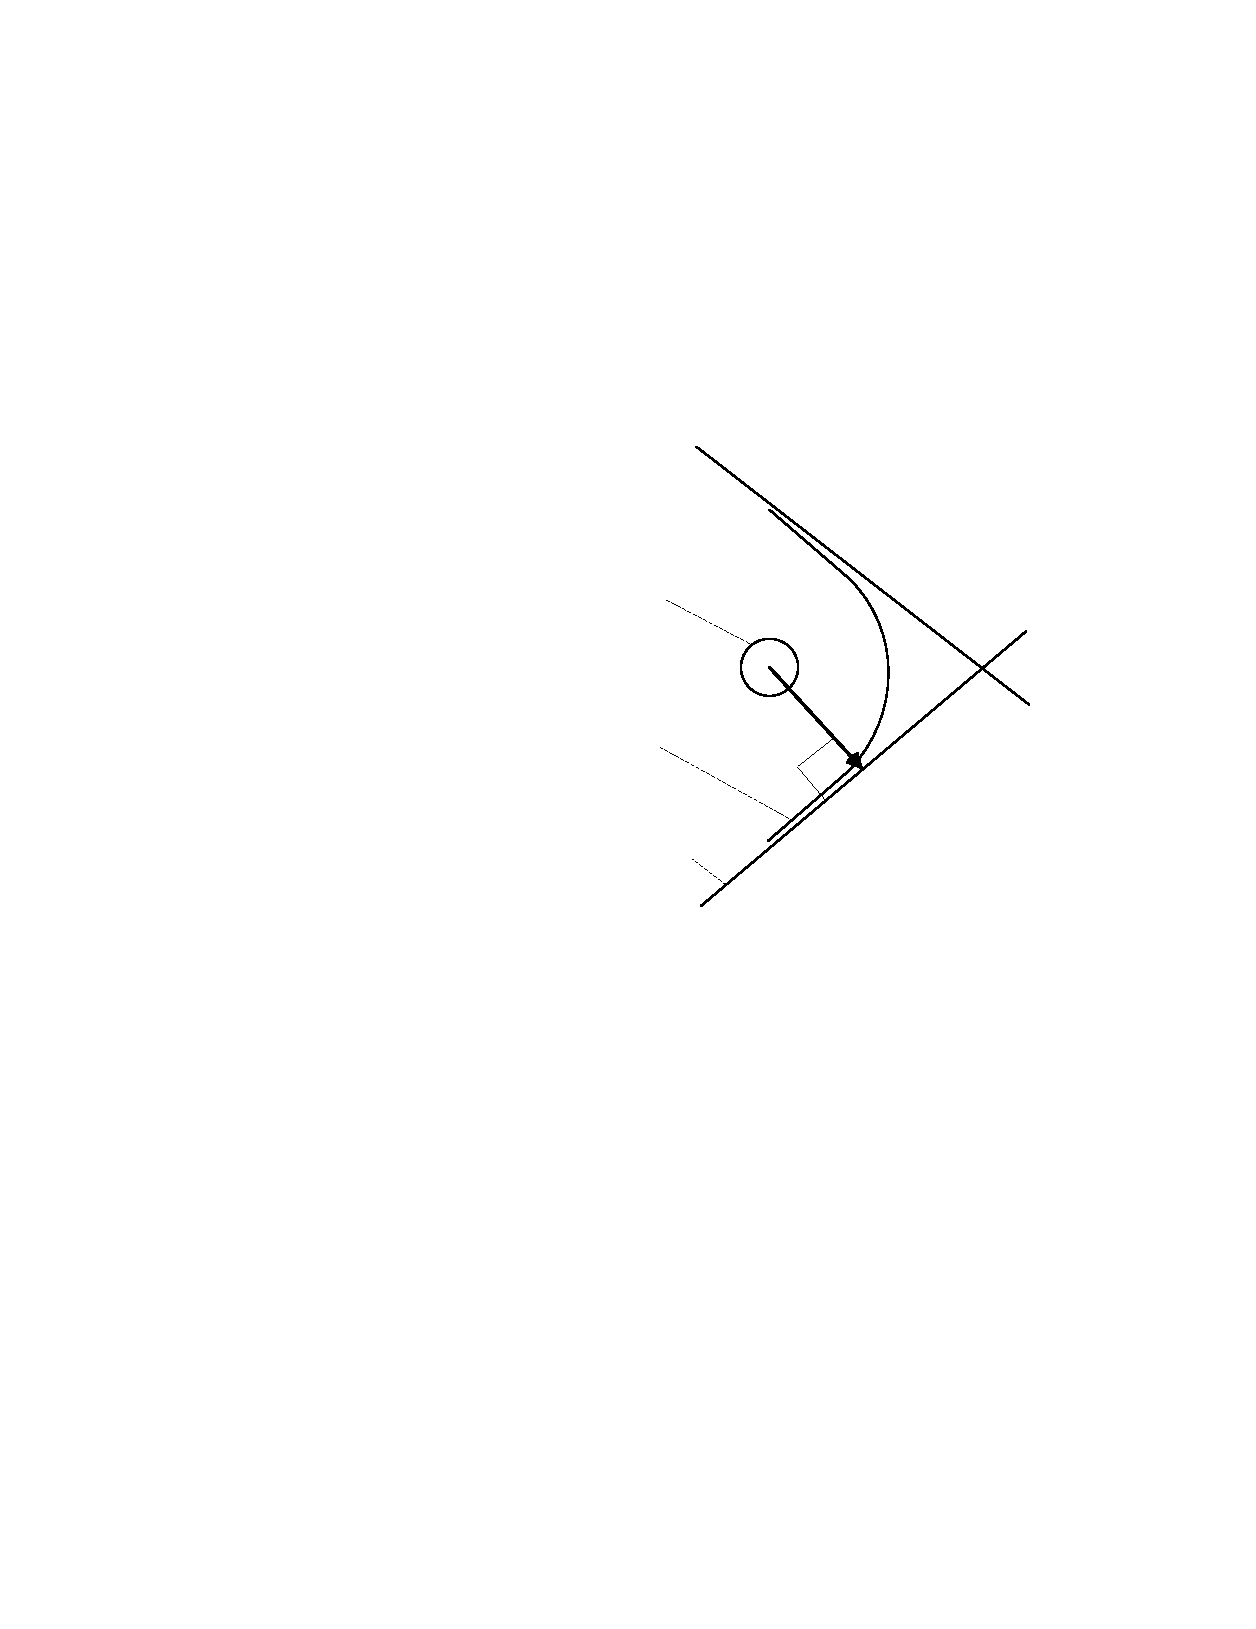
\includegraphics[scale=1]{Images/BPlaneGeometry2.eps}
    \makebox(-420,850){$\mathbf{B}$}
    \makebox(-580,990){Central Body}
    \makebox(-570,850){Incoming Trajectory}
    \makebox(-570,760){Incoming}
    \makebox(-570,740){Asymptote}
    \end{picture}
    \caption{The B-Vector as Seen From a Viewpoint Perpendicular to Orbit Plane}
    \label{fig:BPlaneGeometry2}
\end{figure}

\noindent if $\mathcal{F}_1 \neq \mathcal{F}_B$ convert $\mathbf{r}$
and $\mathbf{v}$ from $\mathcal{F}_1$ to $\mathcal{F}_B$

\[
r = \| \mathbf{r} \|
\]
%
\[
v = \| \mathbf{v} \|
\]
%
Calculate eccentricity related information
%
\[
    \mathbf{e} = \displaystyle\frac{\left( v^2 - \displaystyle\frac{\mu}{r}  \right)\mathbf{r} - (\mathbf{r} \cdot \mathbf{v})\mathbf{v}}{\mu}
\]
%
\[
   e = \| \mathbf{e} \|
\]
%
\[
\hat{\mathbf{e}} = \frac{\mathbf{e}}{e}
\]
%
If $e\leq 1$, then the method fails and returns.

Now let's calculate the angular momentum and orbit normal vectors.
%
\[
\mathbf{h} = \mathbf{r}\times \mathbf{v}
\]
%
\[
h = \| \mathbf{r}\times \mathbf{v} \|
\]
%
\[
\hat{\mathbf{h}} = \frac{\mathbf{h}}{h}
\]

A unit vector normal to both the eccentricity vector and the orbit
normal vector is defined as:
%
\[
   \hat{\mathbf{n}} = \hat{\mathbf{h}} \times \hat{\mathbf{e}}
\]
The following relations are only true for hyperbolic orbits: The
semiminor axis, $b$, can be calculated using
%
\[
   b = \frac{h^2}{\mu \sqrt{e^2 - 1}}
\]
%
The incoming asymptote is defined using
%
\[
   \mathbf{S} =  \frac{\hat{\mathbf{e}} }{e} + \sqrt{1 - \left(\frac{1}{e}\right)^2
   }\hat{\mathbf{n}}
\]
%
The B-vector, $\mathbf{B}$, is calculated using
%
\[
   \mathbf{B} = b \left(\sqrt{1 - \left(\frac{1}{e}\right)^2 }\hat{\mathbf{e}}  - \frac{1}{e} \hat{\mathbf{n}} \right)
\]
%
The remaining vectors, $\mathbf{T}$ and $\mathbf{R}$ are found using
%
\[
   \mathbf{T} = \frac{[\hspace{.03 in} S_y \hspace{.1 in} -S_x  \hspace{.1 in} 0 \hspace{.03 in}]^T }{\sqrt{S_x^2 + S_y^2}}
\]
%
\[
   \mathbf{R} = \mathbf{S} \times \mathbf{T}
\]
%
Finally, the desired quantities are found using
%
\[
   B_T = \mathbf{B} \cdot \mathbf{T}
\]
%
\[
   B_R = \mathbf{B} \cdot \mathbf{R}
\]



\noindent if  $\mathcal{F}_1 \neq \mathcal{F}_2$ , convert
$\mathbf{r}$ and $\mathbf{v}$ to $\mathcal{F}_2$
%
\begin{equation}
    A = \mathbf{r}\cdot\mathbf{v}
\end{equation}

\subsection{BetaAngle} \index{BetaAngle}

Definition:  The Beta angle, $\beta$, is defined as the angle
between the orbit normal vector, and the vector from the celestial
body to the sun.

\[
   \hat{\mathbf{h}} = \frac{  \mathbf{r}_\oplus \times \mathbf{v}_\oplus  }{\|\mathbf{r}_\oplus \times \mathbf{v}_\oplus \|}
\]
%
\[
\hat{\mathbf{r}}_{s \oplus} = \frac{\mathbf{r}_{s \oplus}}{\|_{s
\oplus }  \|}
\]
%
\begin{equation}
  \beta = \sin^{-1}\left(\hat{\mathbf{h}}\cdot \hat{\mathbf{r}}_{s\oplus } \right)
\end{equation}

\begin{itemize}
     \item $\mathbf{r}_\oplus$:  Position vector of spacecraft
     with respect to celestial body, in the EarthMJ2000Eq system.

     \item $\mathbf{v}_\oplus$:  Velocity vector of spacecraft
     with respect to celestial body, in the EarthMJ2000Eq system.

     \item $\mathbf{r}_{s\oplus}$:  Position vector from celestial
     body, to the sun.
\end{itemize}

\subsection{BVectorAngle and BVectorMag} \index{BVectorAngle}
\index{BVectorMag}

To avoid code reduplication, the magnitude and angle of the B
vector, $\|\mathbf{B}\|$ and  $\theta_B$ respectively,  are
calculated from the outputs of the B-Plane coordinates algorithm.
The equations for $\|\mathbf{B}\|$ and $\theta_B$ are
%
\begin{equation}
    \|\mathbf{B}\| = \sqrt{ B_T^2 + B_R^2}
\end{equation}
%
%
\begin{equation}
     \theta_B = \tan^{-1}{\frac{B_R}{B_T}}
\end{equation}
%
which is implemented using $atan2( B_R , B_T )$

\subsection{C3Energy}\index{Spacecraft properties!C3Energy}
\index{C3Energy}

Given:  $a$, and $\mu$

\noindent Find:  $C_3$

\begin{equation}
    C_3 = -\frac{\mu}{a}
\end{equation}

\noindent \textit{Comment}:  $a$ is calculated from the satellite
cartesian state as shown in Section \ref{Sec:Cart2Kep}, and $\mu$ is
associated with the specified central body.

\subsection{DEC} \index{DEC}

\noindent \textit{Description}: \st{DEC} is the declination of a
spacecraft, as shown in Fig. \ref{fig:SphericalElements} using the
symbol $\delta$.

\noindent \textit{Dependency}:  Coordinate System.

\noindent Given:  $\mathbf{r}$, $\mathbf{v}$ and $\mathcal{F}$

\noindent Find:  $\delta$

Begin by converting  $\mathbf{r}$ and $\mathbf{v}$ to  $\mathcal{F}$
if necessary.  Then,
%
\begin{equation}
    r = \| \mathbf{r} \|
\end{equation}
%
\begin{equation}
    \delta = \sin^{-1}(\frac{z}{r})
\end{equation}

\subsection{DECV} \index{DECV}

\noindent \textit{Description}: \st{DECV} is the declination of
velocity of a spacecraft.

\noindent \textit{Dependency}:  Coordinate System.

\noindent Given:  $\mathbf{r}$, $\mathbf{v}$ and $\mathcal{F}$

\noindent Find:  $\delta_v$

Begin by converting  $\mathbf{r}$ and $\mathbf{v}$ to  $\mathcal{F}$
if necessary.  Then,
%
\begin{equation}
       \delta_v = \sin^{-1}(\frac{v_z}{v})
\end{equation}

\subsection{ECC} \index{ECC}

\noindent \textit{Description}: \st{ECC} is the eccentricity  of an
orbit and must be greater than or equal to zero. The eccentricity
contains information on the shape of an orbit. If ECC is zero then
the orbit is circular.  If ECC is greater than zero, but less than
one, the orbit is elliptic. If ECC equals one, the orbit is
parabolic. Finally, if ECC is greater than one, the orbit is
hyperbolic.  The algorithm used in GMAT to calculate SMA is adopted
from Vallado\cite{vallado2}.

\noindent \textit{Dependency}:  Central Body.

\noindent Given:  $\mathbf{r}$, $\mathbf{v}$, and $\mu$ (Central
Body)

\noindent Find:  $e$

%
\begin{equation}
    r = \| \mathbf{r} \|
\end{equation}
%
\begin{equation}
    v = \| \mathbf{v} \|
\end{equation}
%
\begin{equation}
     \mathbf{e} = \displaystyle\frac{(v^2 - \displaystyle\frac{\mu}{r} )\mathbf{r}
     - (\mathbf{r}\cdot\mathbf{v}  )\mathbf{v}}{\mu} \label{Eq:EccentricityVector}
\end{equation}
%
\begin{equation}
     e = \| \mathbf{e} \|
\end{equation}

\subsection{FPA} \index{FPA}

\noindent \textit{Description}: \st{FPA} is the orbit vertical
Flight Path Angle as as shown in Fig. \ref{fig:SphericalElements}
using the symbol $\psi$.

\noindent \textit{Dependency}:  Coordinate System.

\noindent Given:  $\mathbf{r}$, $\mathbf{v}$, and coordinate system
$\mathcal{F}$.

\noindent Find:  $\psi$

Begin by converting  $\mathbf{r}$ and $\mathbf{v}$ to  $\mathcal{F}$
if necessary.  Then,
%
\begin{equation}
    \psi = \cos^{-1}\left(  \frac{\mathbf{r} \cdot \mathbf{v} }{r v} \right)
\end{equation}
%

\subsection{EA} \label{sec:EccentricAnomaly}
\index{EA}

Given: $\nu$, $e$

\noindent Find:  $E$\\
%

\noindent If e $>$ ( 1 - $1e^{-11}$ ) then $E = 0$, return.\\
%


\noindent Otherwise,
%
\begin{eqnarray}
    \sin(E) & = & \frac{\sqrt{1 - e^2} \sin(\nu)}{1+e \cos{\nu}}    \\    %Vallado pg. 213,  Eq. 4-9
    %
    \cos(E) & = & \frac{ e + \cos{\nu} }{1+e \cos{\nu}}   \\     %Vallado pg. 213,  Eq. 4-9
    %
    E & = & \mbox{atan2}(\sin{E},\cos{E})
\end{eqnarray}
%

\subsection{Energy}\index{Spacecraft properties!Energy}
\index{Energy}

\noindent \textit{Description}: \st{Energy} is the orbit energy.

\noindent \textit{Dependency}:  Central Body.

\noindent Given:  $\mathbf{r}$, $\mathbf{v}$, and central body.

\noindent Find:  $\xi$

Begin by converting $\mathbf{r}$ and $\mathbf{v}$ to a coordinate
system with the origin equal to the central body defined by the
user, and the MJ2000Eq axis system.  Then,
%
\begin{equation}
     r = \mathbf{r}
\end{equation}
%
\begin{equation}
     v = \mathbf{v}
\end{equation}
%
\begin{equation}
    \xi = \frac{v^2}{2} - \frac{\mu}{r}
\end{equation}


\subsection{HMAG} \index{HMAG}

\noindent \textit{Description}: \st{HMAG} is the magnitude of the
orbit angular momentum.

\noindent \textit{Dependency}:  Central Body.

\noindent Given:  $\mathbf{r}$, $\mathbf{v}$, and central body.

\noindent Find:  $h$

Begin by converting $\mathbf{r}$ and $\mathbf{v}$ to a coordinate
system with the origin equal to the central body defined by the
user, and the MJ2000Eq axis system.  Then,
%
\begin{equation}
    \mathbf{h} = \mathbf{r} \times \mathbf{v}
\end{equation}
%
\begin{equation}
    h = \| \mathbf{h} \|
\end{equation}

\subsection{HX,HY, and HZ} \index{HX} \index{HY} \index{HZ}

\noindent \textit{Description}: \st{HX,HY,} and \st{HZ} are the
components of the orbit angular momentum vector.

\noindent \textit{Dependency}:  Coordinate System.

\noindent Given:  $\mathbf{r}$, $\mathbf{v}$, and coordinate system
$\mathcal{F}$.

\noindent Find:  $h_x$, $h_y$, and $h_z$

Begin by converting $\mathbf{r}$ and $\mathbf{v}$ to $\mathcal{F}$
if necessary. Then,
%
\begin{equation}
    \mathbf{h} = \mathbf{r} \times \mathbf{v} = [\hspace{.05 in} h_x
    \hspace{.1 in} h_y \hspace{.1 in} h_z \hspace{.05 in} ]^T
\end{equation}


\subsection{HA}  \label{sec:HyperbolicAnomaly}
\index{HA}

\noindent \textit{Description}: \st{HA} is the orbit Hyperbolic
Anomaly and is only defined for hyperbolic orbits.  For
non-hyperbolic orbits, \st{HA} returns a value of zero.

\noindent \textit{Dependency}:  Central Body.
 Given: $\nu$, $e$

\noindent Find:  $H$\\
%

\noindent If e $<$ ( 1 + $1e^{-11}$ ) then $H = 0$, return.\\
%


\noindent Otherwise,
%
\begin{eqnarray}
    \sinh(H) & = & \frac{ \sin(\nu) \sqrt{e^2 - 1}}{1+e \cos{\nu}}    \\    %Vallado pg. 213,  Eq. 4-9
    %
    H & = & \mbox{asinh}(\sinh(H))
\end{eqnarray}
%

\subsection{INC} \index{INC}

\noindent \textit{Description}: \st{INC} is the inclination of an
orbit in the chosen coordinate system.

\noindent \textit{Dependency}:  Coordinate System.

\noindent Given:  $\mathbf{r}$, $\mathbf{v}$, and coordinate system
$mathcal{F}$.

\noindent Find:  $e$

Begin by converting  $\mathbf{r}$ and $\mathbf{v}$ to  $mathcal{F}$
if necessary.  Then,
%
\begin{equation}
     \mathbf{h} = \mathbf{r} \times \mathbf{v}
\end{equation}
%
\begin{equation}
      h  = \mathbf{h}
\end{equation}
%
\begin{equation}
     i = \cos^{-1}( \frac{h_z}{h} )
\end{equation}


\subsection{Latitude} \label{Sec:Latitude} \index{Latitude}

\noindent \textit{Description}: \st{Latitude} is the geodetic
latitude of a spacecraft.  The geodedic latitude is defined as the
the angle $\phi_{gc}$, as shown in Fig. ( ),  where the
sub-satellite point is defined by the interscection of a line drawn
from the spacecraft and perpendicular to a plane tangent to the
surface of the body. GMAT assumes the body is an ellipsoid. The
equatorial radius, and properties of the ellipsoid depend upon the
particular body chosen by the user.  The algorithm in GMAT is taken
from Vallado\cite{vallado2}.

\begin{figure}[htb]
    \begin{picture}(100,200)(75,320)
        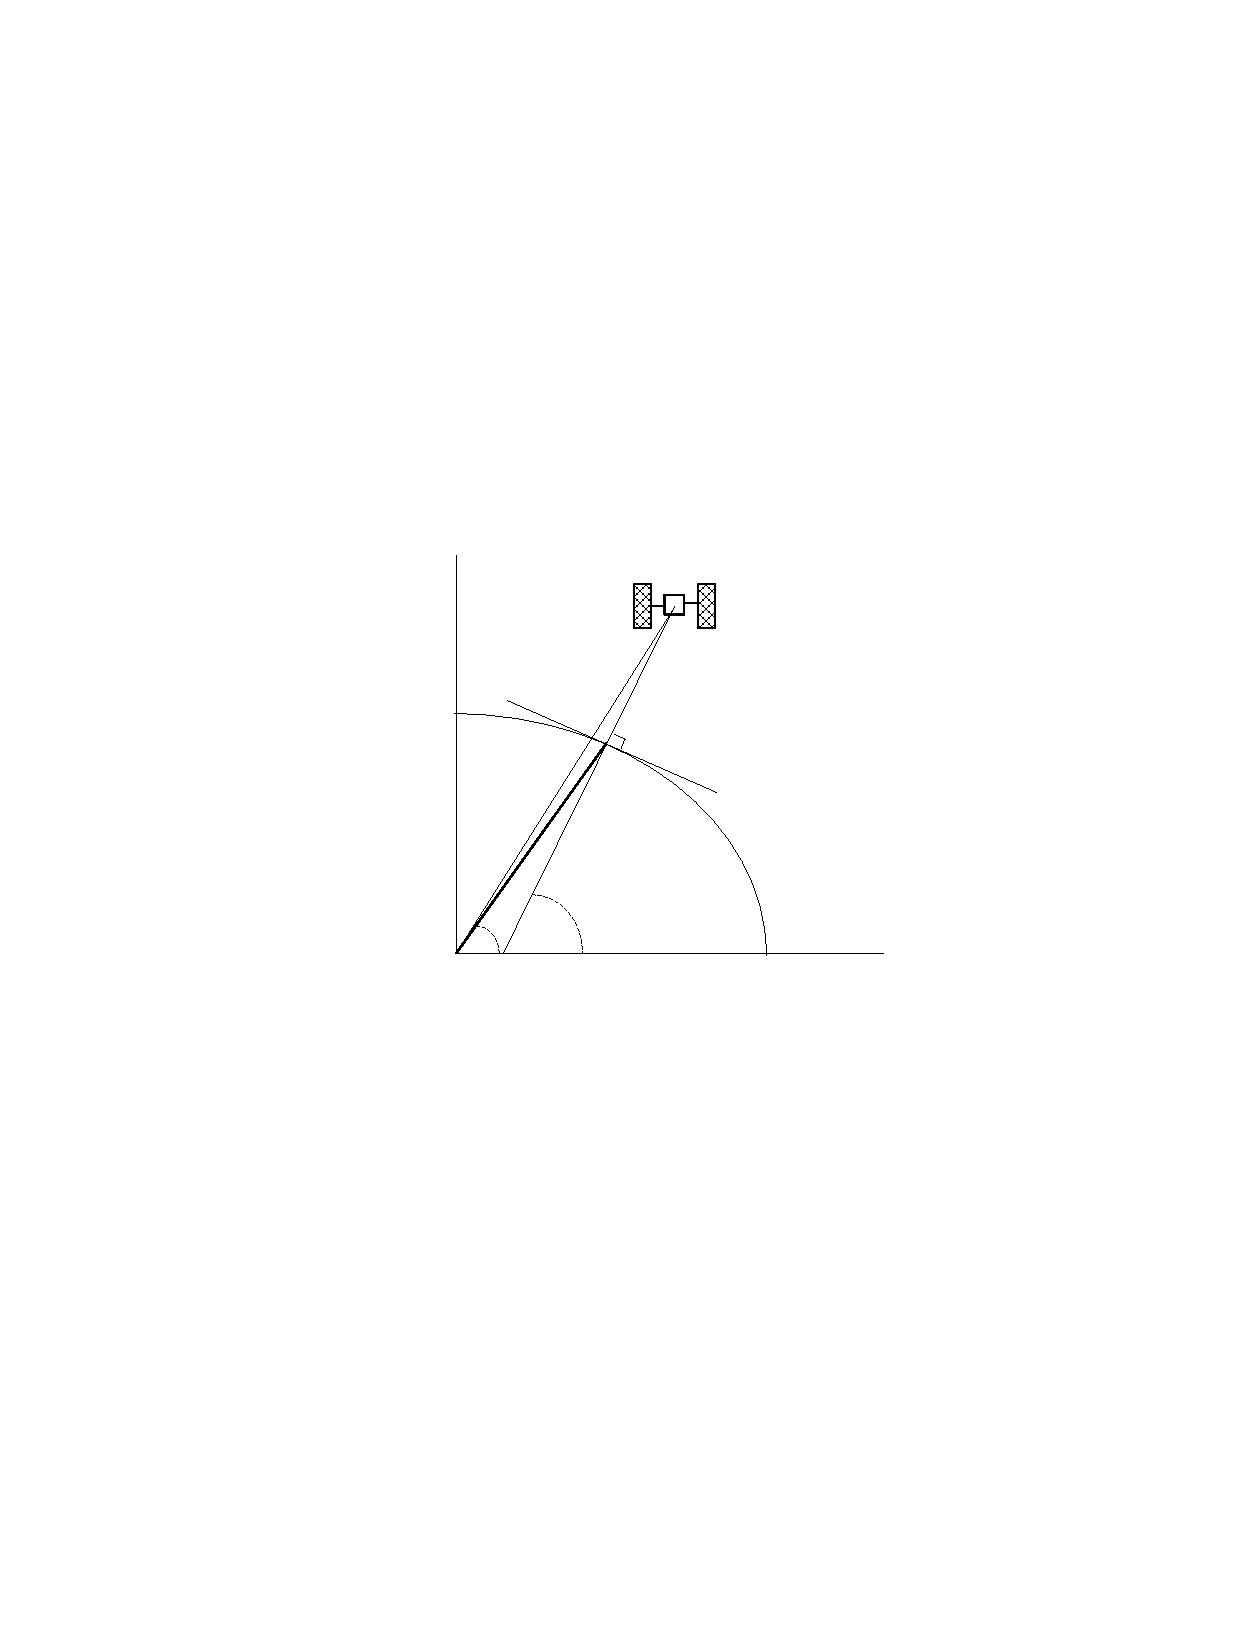
\includegraphics[scale=1]{Images/GeodeticDiagram.eps}
    \makebox(-575,880){$h$}
    \makebox(-640,680){$\phi_{gd}$}
    \makebox(-730,670){$\phi_{gc}$}
    \end{picture}
    \caption{Geocentric and Geodetic Latitude}
    \label{fig:GeodeticDiagram}
\end{figure}

\noindent \textit{Dependency}:  Central Body.

\noindent Given:  $\mathbf{r}$ in $\mathcal{F}_1$

\noindent Find:  $\phi_{gc}$

\noindent Definitions:
\begin{itemize}
     %
     \item $\mathcal{F}_1$ is the coordinate system in which GMAT originally knows $\mathbf{r}$
     %
     \item $\mathcal{F}_F$ is body fixed system of the central body selected by the user.
     %
     \item $f$ is the bodies flattening coefficient
     %
     \item $R$ is the bodies mean equatorial radius
     %
     \item $\phi_{gd}$ is the geodedic latitude of the spacecraft
     in the body fixed frame.
     %
\end{itemize}
%
if $\mathcal{F}_1 \neq \mathcal{F}_F$ convert $\mathbf{r}$ from
$\mathcal{F}_1$ to $\mathcal{F}_F$. Then,
%
\begin{equation}
     r_{xy} = \sqrt{ x^2 + y^2 }
\end{equation}
%
Calculate the geocentric latitude to use as an initial guess to find
the geodetic latitude
%
\begin{equation}
     \phi_{gd}  \approx \mbox{atan2}(z,  r_{xy}  );
\end{equation}
%
\begin{equation}
    e^2 = 2f-f^2
\end{equation}
%

\noindent Set $\delta = 1.0$ to initialize the loop, then,


\noindent While ( $\delta > 10^{-7}$ )
%
\begin{eqnarray}
   \phi' & = & \phi_{gd}\\
   %c & = & \frac{R} { \sqrt{1 - e^2\sin{\phi}}    }\\
   \phi_{gd} & = & \mbox{atan2}\left(z +  \frac{Re^2\sin^{2}{\phi_{gd}}} { \sqrt{1 - e^2\sin{\phi_{gd}}} }, r_{xy}
   \right)\\
   \delta & = & | \phi_{gd} - \phi' |
\end{eqnarray}
%
EndWhile\\
%

After convergence, $\phi_{gd}$ is converted to degrees, and
converted to fall between $-90^\circ$ and   $+90^\circ$ degrees.

\subsection{Longitude} \label{Sec:CalcObjectLongitude}
\index{Longitude}

\noindent \textit{Description}: \st{Longitude} is the longitude of
an object, in the body fixed frame of the central body chosen by the
user.

\noindent \textit{Dependency}:  Central Body.

\noindent Given:  $\mathbf{r}$, central body.

\noindent Find:  $\phi$

Begin by converting $\mathbf{r}$ to the body fixed system of the
central body defined by the user. Then,
%
\begin{equation}
    \phi = \tan_2^{-1}(y,x);
\end{equation}
%
The calculation is completed by converting to degrees and setting
the value to such that $-180 \leq \phi < 180$.

\subsection{LST} \index{LST}

\noindent \textit{Description}: \st{LST} is the local sidereal time
of an object, with respect to the selected central body.  The local
sidereal time is the sum of the longitude in the bodies fixed frame,
and the mean sidereal time.  This is illustrated in Fig.
\ref{fig:SiderealTimeDiagram}, where $\mathcal{F}_I$ is the body's
equatorial inertial system (as described in Sec. \ref{Sec:Equator}),
$\mathcal{F}_F$ is the body's fixed system (as described in Sec.
\ref{Sec:Fixed}).  $\lambda$ is the longitude of the object, in this
case a spacecraft, and $\theta_{MST}$ is the mean sidereal time of
the prime meridian.

\noindent \textit{Dependency}:  Central Body.

\noindent Given:  $\mathbf{r}$, $t_i$ (epoch of spacecraft in
internal time system), and central body

\noindent Find:  $\theta_{LST}$

\noindent Definitions:
\begin{itemize}
     %
     \item $\mathcal{F}_I$ equatorial inertial system (as described in Sec. \ref{Sec:Equator}) of selected central
     body.
     %
     \item $\mathcal{F}_F$ is the central body's fixed system (as described in Sec. \ref{Sec:Fixed})
     %
     \item $\lambda$ is the longitude of the object in $\mathcal{F}_F$
     %
     \item $\theta_{MST}$ is the mean sidereal time of the central body's  prime meridian.
     %
     \item $t_i$ (epoch of spacecraft in internal time system)
\end{itemize}

\begin{figure}[htb]
    \begin{picture}(100,230)(55,460)
        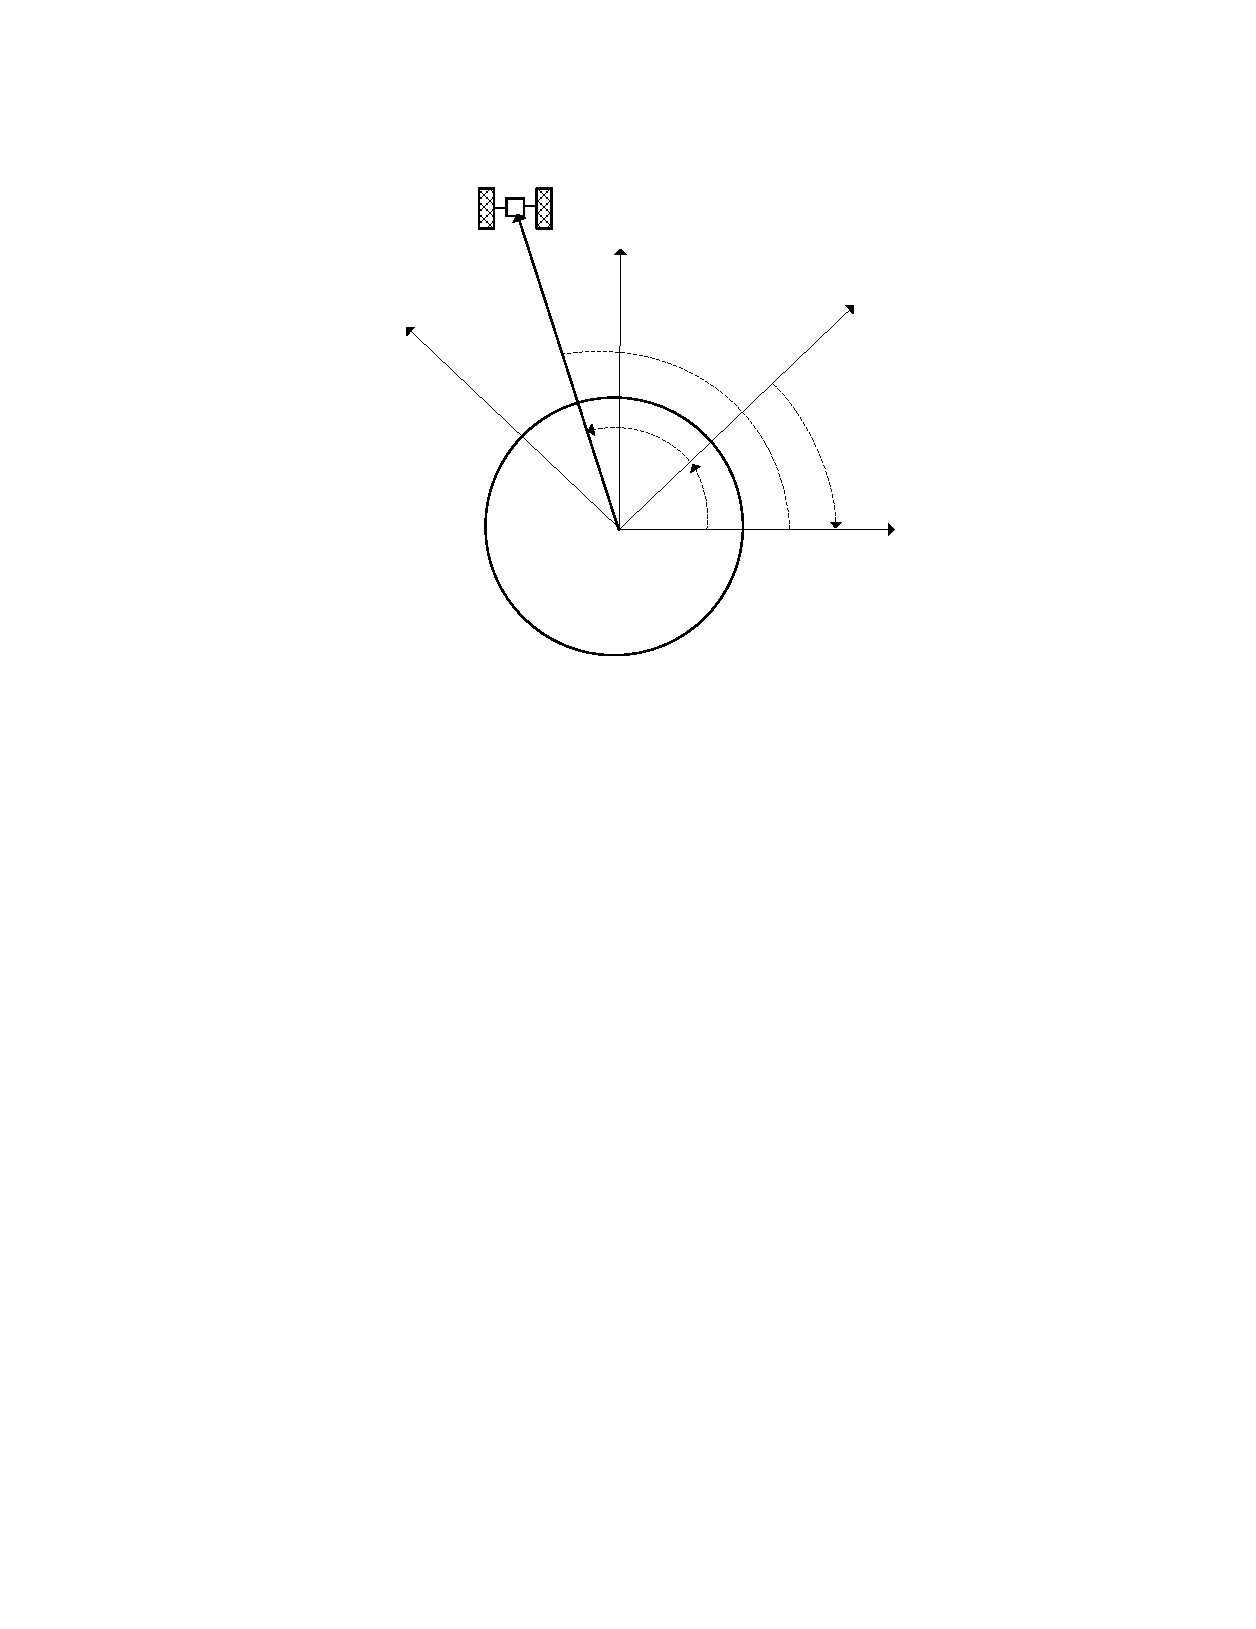
\includegraphics[scale=1]{Images/SiderealTimeDiagram.eps}
    \makebox(-350,1066){$\hat{\mathbf{x}}_I$}
    \makebox(-380,1277){$\hat{\mathbf{x}}_F$}
    \makebox(-617,1330){$\hat{\mathbf{y}}_I$}
    \makebox(-800,1240){$\hat{\mathbf{y}}_F$}
    \makebox(-575,1059){$\theta_{MST}$}
    \makebox(-600,1120){$\lambda$}
    \makebox(-580,1220){$\theta_{LST}$}
    \makebox(-425,1125){$\theta_{MHA}$}
    \end{picture}
    \caption{Local Sidereal Time Geometry}
    \label{fig:SiderealTimeDiagram}
\end{figure}

We begin by calculating $\lambda$ using the algorithm described in
Sec. \ref{Sec:CalcObjectLongitude}.  The mean sidereal time
$\theta_{MST}$ is calculated differently for Earth than for other
central bodies.  If the central body is Earth, then we use the
following equations to calculate $\theta_{MST}$.

First, convert $t_i$, which is the spacecraft epoch in the interal
time system (A1 Modified Julian Date), to $T_{UT1}$, which is the
number elapsed Julian centuries from the J2000 epoch.
%
\begin{equation}
    T_{UT1} = \frac{t_{ut1} - 21544.5}{36525}
\end{equation}
%
\begin{equation}\begin{split}
    \theta_{MST} =  & 67310.54841^s + \\ &( 876600^h \left( \frac{3600 s}{1h}\right) + 8640184.812866)T_{UT1} + \\& 0.093104T_{UT1}^2 - 6.2\times10^{-6}T_{UT1}^3
    \end{split}
\end{equation}

\subsection{MA} \index{MA}

Given: $\nu$, $e$

\noindent Find:  $M$

\noindent If e $<$ ( 1 - $1e^{-11}$ ) then calculate $E$ using
algorithm in Sec. \ref{sec:EccentricAnomaly}.  Then $M$ is
calculated using
%
\begin{equation}
     M = E - e \sin{E}
\end{equation}
%
Note: $E$ must be expressed in radians in the above equation, and
results in $M$ in radians.

\noindent If e $>$ ( 1 + $1e^{-11}$ ) then calculate $H$ using
algorithm in Sec. \ref{sec:HyperbolicAnomaly}.  Then $M$ is
calculated using
%
\begin{equation}
     M =  e \sinh{H} - H
\end{equation}
%
Note: $H$ must be expressed in radians in the above equation, and
results in $M$ in radians.  GMAT outputs \st{MA} in degrees.

\noindent If neither of the above conditions are satisfied, $M = 0$,
and output ``Warning:  Orbit is near parabolic in mean anomaly
calculation. Setting MA = 0".

\subsection{MHA}

\subsection{MM}\index{Spacecraft properties!mean motion}
\index{MM}

Given:  $a$, $e$, and $\mu$

\noindent Find:  $n$

\noindent The orbit is considered either circular or elliptic ( both
orbit types use the same equation to calculate $n$) if $ e < 1 -
1e^{-11}$. In this case the mean motion, $n$, is calculated using
%
\begin{equation}
    n = \sqrt{\frac{\mu}{a^3}}
\end{equation}
%
The orbit is considered hyperbolic if $ e > 1 + 1e^{-11}$.  In this
case the mean motion, $n$, is calculated using
%
\begin{equation}
    n =  \sqrt{-\frac{\mu}{a^3}}
\end{equation}
%
If neither of the above two conditions are met, the mean motion is
calculated using
%
%
\begin{equation}
    n =  2\sqrt{\mu}
\end{equation}
%

\noindent \textit{Comment}:  $a$ and $e$ are calculated from the
satellite cartesian state as shown in Section \ref{Sec:Cart2Kep},
and $\mu$ is associated with the specified central body.


\subsection{OrbitPeriod}\index{Spacecraft properties!OrbitPeriod}
\index{OrbitPeriod}

Given:  $a$, and $\mu$

\noindent Find:  $T$

\noindent If a $ < 0$,  then $T = 0$, return.\\
%


\noindent Otherwise,
\begin{equation}
    T = 2\pi\sqrt{\frac{a^3}{\mu}}
\end{equation}

\noindent \textit{Comment}:  $a$ is calculated from the satellite
cartesian state as shown in Section \ref{Sec:Cart2Kep}, and $\mu$ is
associated with the specified central body.

\subsection{PercentShadow } \label{sec:PercentShadow}
\index{PercentShadow}

The \st{PercentShadow} parameter calculates the percentage of the
apparent solar disk that is in view from the perspective of a
spacecraft. The algorithm used in GMAT was adapted from
Montenbruck\cite{Montenbruck:Gill:05} pgs. 80-83.

\begin{figure}[htb]
    \begin{picture}(100,220)(65,275)
        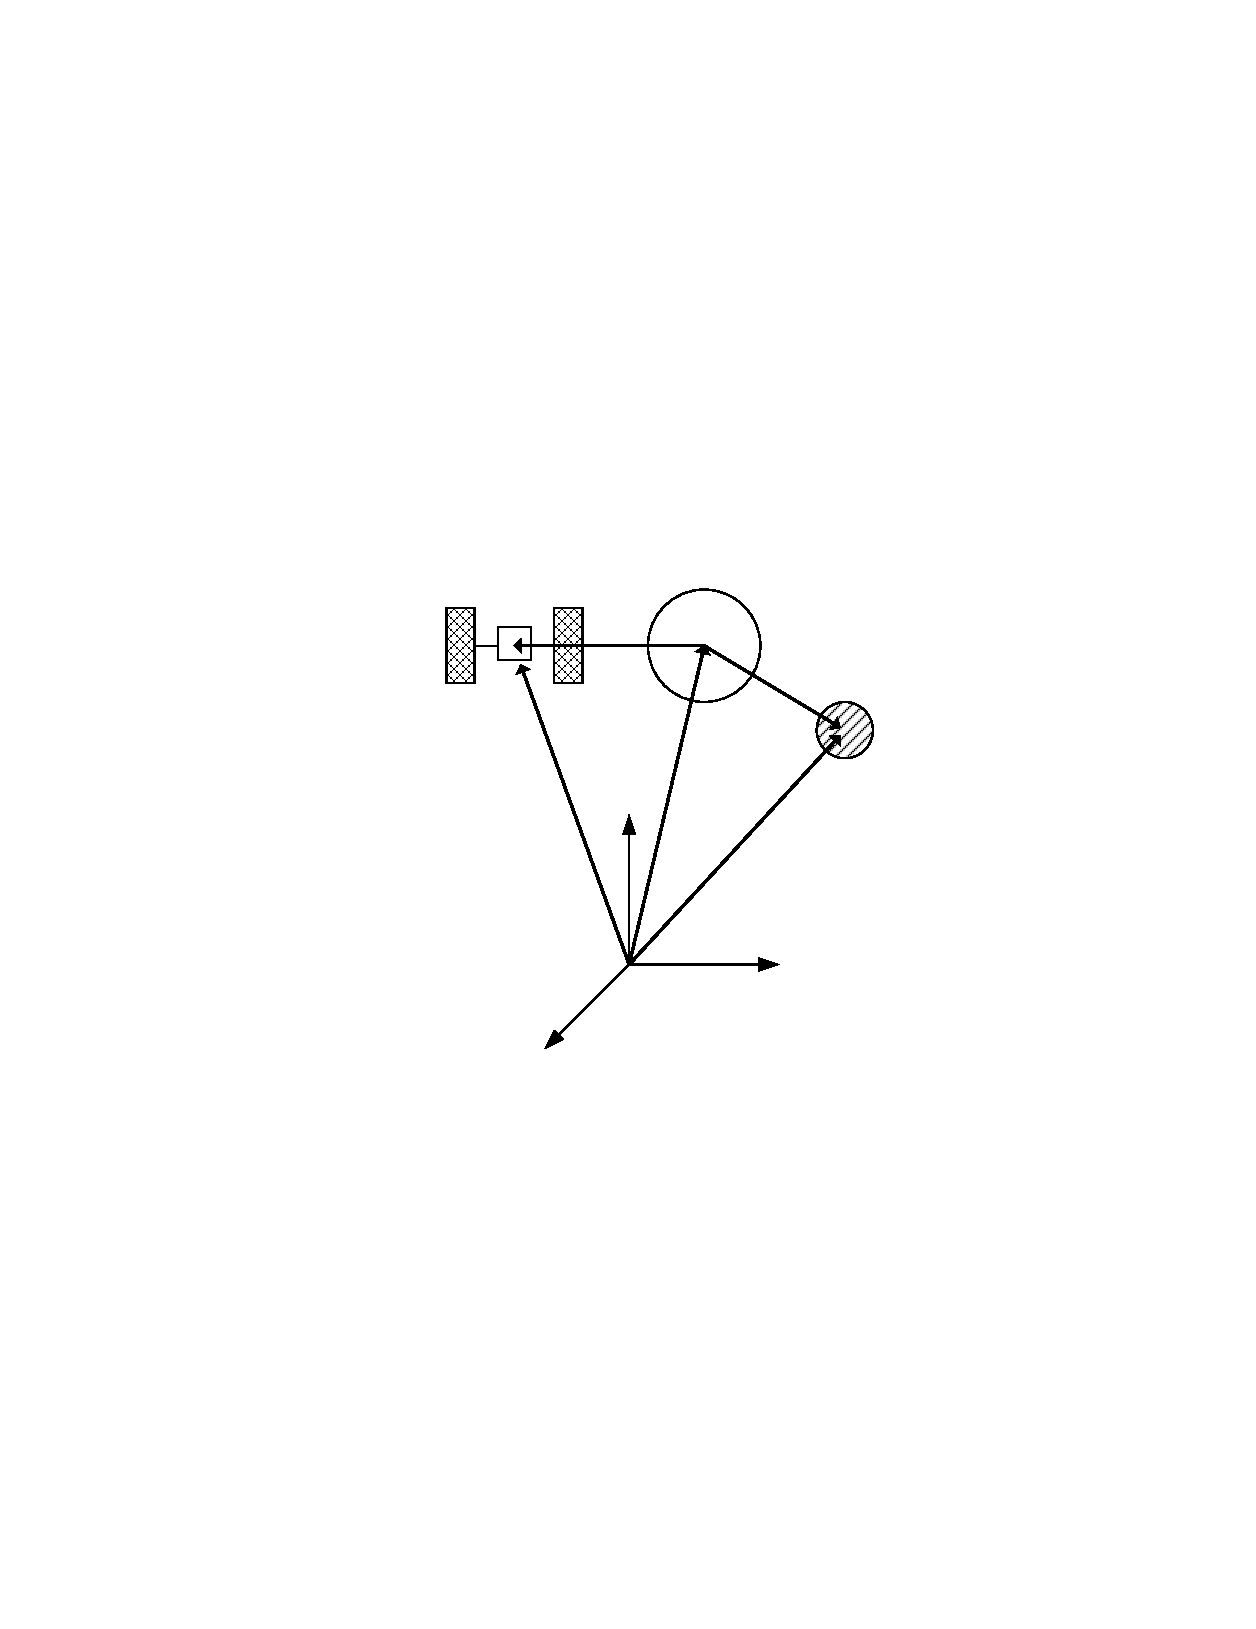
\includegraphics[scale=1]{Images/ShadowGeometry.eps}
    \makebox(-520,850){$\mathbf{r}_B$}
    \makebox(-460,750){$\mathbf{r}_\odot$}
    \makebox(-690,800){$\mathbf{r}$}
     \makebox(-620,940){$\mathbf{s}$}
     \makebox(-450,890){$\mathbf{s}_\odot$}
    \end{picture}
    \caption{Shadow Geometry}
    \label{fig:ShadowGeometry}
\end{figure}
%
\begin{itemize}
    \item $R_\odot$ = Radius of the Sun
    \item $R_B$ = Radius of occulting body
    \item $R'_\odot$ = Apparent radius of the Sun
    \item $R'_B$ = Apparent radius of occulting body
    \item $\mathbf{r}_\odot$ = Vector from central body to Sun
    \item $\mathbf{r}_B$ = Vector from central body to occulting body
    \item $\mathbf{r}$ = Vector from central body to s/c
\end{itemize}
%

We begin by calculating the vector from the occulting body to the
spacecraft, $\mathbf{s}$, using
%
\begin{equation}
     \mathbf{s} = \mathbf{r} - \mathbf{r}_B
\end{equation}
%
and the vector from the occulting body to the sun,
$\mathbf{s}_\odot$, using
%
\begin{equation}
     \mathbf{s}_\odot = \mathbf{r}_\odot - \mathbf{r}_B
\end{equation}
%
(Note that when the occulting body is the same as the central body,
$\mathbf{s} = \mathbf{r}$, and $\mathbf{s}_\odot =
\mathbf{r}_\odot$)

Next we calculate the apparent radius of the Sun and occulting body
using
%
\begin{eqnarray}
     R'_\odot & = & \sin^{-1}\frac{R_\odot}{\|\mathbf{r}_\odot - \mathbf{r} \|}\\
     R'_B & = & \sin^{-1}\frac{R_B}{\|\mathbf{r}  - \mathbf{r}_B\|}
\end{eqnarray}
%
We can calculate the apparent separation of the two bodies, $D'$,
using
%
\begin{equation}
    D' = \cos^{-1}\left(\frac{-\mathbf{s}^T\left( \mathbf{r}_\odot - \mathbf{r} \right)}{s \|\mathbf{r}_\odot - \mathbf{r}
    \|}\right)
\end{equation}
%

If $ D' \geq R'_\odot + R'_B $, then the spacecraft is not in the
body's shadow and
%
\begin{equation}
    p = 0;
\end{equation}
%

If $D' \leq R'_B - R'_\odot$, then the spacecraft is in full shadow
and
%
\begin{equation}
    p = 100;
\end{equation}
%

If neither of the above conditions are met, the spacecraft is in
partial shadow.
%
\begin{figure}[htb]
    \begin{picture}(100,135)(35,355)
        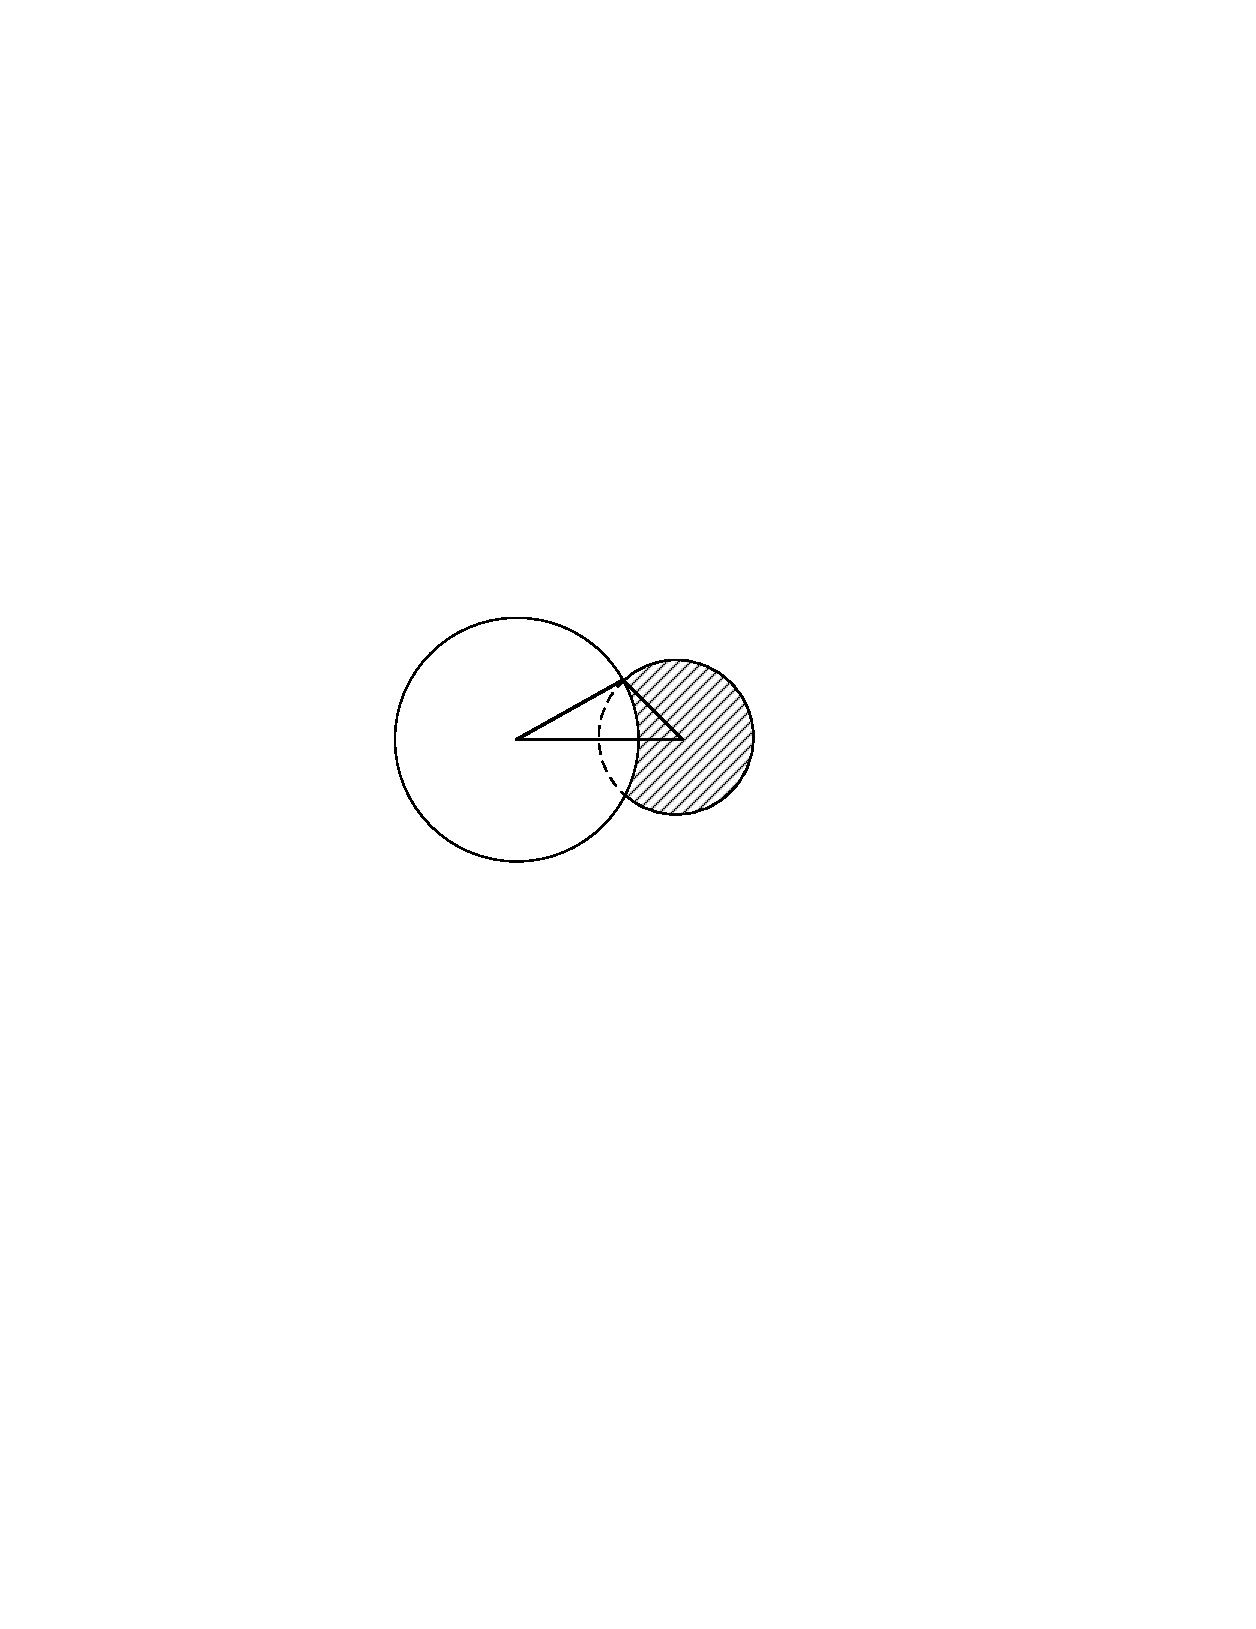
\includegraphics[scale=1]{Images/ShadowIllustration.ps}
            \makebox(-650,895){$R'_B$}
            \makebox(-550,870){$R'_\odot$}
            \makebox(-670,820){$D'$}
            \makebox(-560,750){Sun}
            \makebox(-720,765){Occulting Body}
    \end{picture}
    \caption{Occultation Geometry in Calculation of PercentShadow}
    \label{fig:ShadowIllustration}
\end{figure}
%

If $|R'_s - R'_B| < D' < R'_s + R'_B$, then we can calculate the
percentage of shadow by calculating the area of overlap, $A$,  of
the two apparent disks as shown in Fig.
\ref{fig:ShadowIllustration}.
%
\begin{equation}
     A = R^{'\mbox{} 2}_\odot\cos^{-1}\left(\frac{c_1}{R'_\odot}\right) +
     R^{'\mbox{} 2}_B\cos^{-1}\left(\frac{D' - c_1}{R'_B}\right) -
     D'c_2
\end{equation}
%
where
%
\begin{equation}
   c_1 = \frac{ D^{'\mbox{} 2} + R^{'\mbox{} 2}_\odot - R^{'\mbox{} 2}_B }{2D'}
\end{equation}
%
and
%
\begin{equation}
   c_2 = \sqrt{ R^{'\mbox{} 2}_\odot -  c_1^2 }
\end{equation}
%
The percent  shadow can be calculated using
%
\begin{equation}
     p = 100 \frac{A}{\pi R^{'\mbox{} 2}_\odot}
\end{equation}

If the condition $|R'_\odot - R'_B| < D' < R'_\odot + R'_B$ is not
satisfied, then the eclipse is annular and we use
%
\begin{equation}
     p = 100   \frac{R^{'\mbox{} 2}_B}{R^{'\mbox{} 2}_\odot}
\end{equation}


\subsection{RA}\index{RA}

\noindent \textit{Description}: \st{RA} is the right ascension of a
spacecraft, as shown in Fig. \ref{fig:SphericalElements} using the
symbol $\lambda$.

\noindent \textit{Dependency}:  Coordinate System.

\noindent Given:  $\mathbf{r}$, $\mathbf{v}$ and $\mathcal{F}$

\noindent Find:  $\lambda$

Begin by converting  $\mathbf{r}$ and $\mathbf{v}$ to  $\mathcal{F}$
if necessary.  Then,
%
\begin{equation}
    \lambda= \tan^{-1}_2(y,x)
\end{equation}

\subsection{RAV} \index{RAV}

\noindent \textit{Description}: \st{RAV} is the right ascension of
velocity of a spacecraft, as shown in Fig.
\ref{fig:SphericalElements} using the symbol $\lambda_v$.

\noindent \textit{Dependency}:  Coordinate System.

\noindent Given:  $\mathbf{r}$, $\mathbf{v}$ and $\mathcal{F}$

\noindent Find:  $\lambda_v$

Begin by converting  $\mathbf{r}$ and $\mathbf{v}$ to  $\mathcal{F}$
if necessary.  Then,
%
\begin{equation}
    \lambda_v= \tan^{-1}_2(v_y,v_x)
\end{equation}


\subsection{RAAN} \index{RAAN}

\noindent \textit{Description}: \st{RAAN} is the right ascension of
the ascending node as shown in Fig. \ref{fig:KeplerianElements}
using the symbol $\Omega$.

\noindent \textit{Dependency}:  Coordinate System.

\noindent Given:  $\mathbf{r}$, $\mathbf{v}$, and coordinate system
$\mathcal{F}$.

\noindent Find:  $e$

Begin by converting  $\mathbf{r}$ and $\mathbf{v}$ to  $\mathcal{F}$
if necessary.  Then,
%First calculate the specific angular momentum and its magnitude.
\begin{equation}
     \mathbf{h} = \mathbf{r} \times \mathbf{v}
\end{equation}
%
\begin{equation}
     h = \|\mathbf{h} \|
\end{equation}
%
\begin{equation}
     \mathbf{n} = [ \hspace{0.05 in} 0 \hspace{0.1 in} 0 \hspace{0.1 in} 1 \hspace{0.05
     in}]^T \times \mathbf{h}
\end{equation}
%
\begin{equation}
     n = \| n\|
\end{equation}
%
\begin{equation}
     i = \cos^{-1}\left(\frac{h_z}{h}\right)
\end{equation}
%


\noindent if  $(i \geq 10^{-11})$, then
%
\begin{equation}
    \Omega = \cos^{-1}\left(\frac{n_x}{n}\right)
\end{equation}
%
Fix quadrant for $\Omega$: if $n_y < 0$, then $\Omega = 2\pi -
\Omega$


\noindent if  $(i < 10^{-11})$, then
%
\begin{equation}
    \Omega = 0
\end{equation}


\subsection{RadApo}\index{Spacecraft properties!RadApo}
\index{RadApo}

Given:  $a$, and $e$

\noindent Find:  $r_a$

\noindent  if $ 1 - e  < 10^{-12}$  then $r_a = 0$.  Note, this
means that for parabolica, and hyperbolic orbits, GMAT outputs a
value of zero for \st{RadApo}.
%
\noindent Otherwise,
%
\begin{equation}
    r_a = a(1+e)
\end{equation}

\noindent \textit{Comment}:  $a$ and $e$ are calculated from the
satellite cartesian state as shown in Section \ref{Sec:Cart2Kep}.

\subsection{RadPer}\index{Spacecraft properties!RadPer}
\index{RadPer}

Given:  $a$, and $e$

\noindent Find:  $r_p$

\begin{equation}
    r_p = a(1-e)
\end{equation}

\noindent \textit{Comment}:  $a$ and $e$ are calculated from the
satellite cartesian state as shown in Section \ref{Sec:Cart2Kep}.

\subsection{RLA and DLA} \index{RLA} \index{DLA}

\noindent \textit{Description}: \st{RLA} ($\lambda_s$) is the right ascenstion of the outgoing
asypmptote of a hyperbolic trajectory.  \st{DLA} ($\delta_s$)is the declination of the outgoing
asypmptote of a hyperbolic trajectory.

\noindent \textit{Dependency}:  Coordinate System.

\noindent Given:  $\mathbf{r}$ and $\mathbf{v}$ and desired coordinate system.

\noindent Find:  $\lambda_s$ and $\delta_s$

Begin by converting $\mathbf{r}$ and $\mathbf{v}$ to the desired coordinate system (an excpeption
is thrown if the origin of the requested coordinate system is not a celestial body).
The eccentricity vector $\mathbf{e}$ is computed using Eq.~(\ref{Eq:EccentricityVector}).
If $\|\mathbf{e}\| < 1 + tol$ then RLA = DLA = NaN and return. Otherwise:
%
\begin{equation}
    \mathbf{h} = \mathbf{r} \times \mathbf{v}
\end{equation}
%
\begin{equation}
    h = \| \mathbf{h} \|
\end{equation}
%
\begin{equation}
   C_3 = v^2 - \frac{2\mu}{r}
\end{equation}
%
where $\mu$ is gravitational parameter of the central body at the origin of the given coordinate system.   The outgoing asmympote unit vector, $\hat{\mathbf{s}} $, is computed using
%
\begin{equation}
   \hat{\mathbf{s}} = \frac{1}{ 1 + C_3 \displaystyle\left(\frac{h}{\mu}\right)^2}\left(   \frac{\sqrt{C_3}}{\mu} \left(\mathbf{h} \times \mathbf{e} \right) - \mathbf{e} \right)
\end{equation}
%
RLA and DLA are computed from
%
\begin{equation}
    \lambda_s = \tan^{-1}(s_y,s_x)
\end{equation}
%
\begin{equation}
    \delta_s = \sin^{-1}(s_z)
\end{equation}

\subsection{RMAG} \index{RMAG}

\noindent \textit{Description}: \st{RMAG} is the magnitude of the
spacecraft's position vector.

\noindent \textit{Dependency}:  Central Body.

\noindent Given:  $\mathbf{r}$ and central body.

\noindent Find:  $r$

Begin by converting $\mathbf{r}$  to a coordinate system with the
origin equal to the central body defined by the user, and the
MJ2000Eq axis system.  Then,
%
\begin{equation}
    r = \| \mathbf{r} \|
\end{equation}

\subsection{SemilatusRectum} \index{SemilatusRectum}

\noindent \textit{Description}: \st{SemilatusRectum} is the orbit
semilatus rectum, which is the magnitude of the position vector,
when at true anomaly of $90^{\circ}$.

\noindent \textit{Dependency}:  Central Body.

\noindent Given:  $\mathbf{r}$, $\mathbf{v}$, and $\mu$ (central
body).

\noindent Find:  $p$

Begin by converting $\mathbf{r}$ and $\mathbf{v}$ to a coordinate
system with the origin equal to the central body defined by the
user, and the MJ2000Eq axis system.  Then,
%
\begin{equation}
    \mathbf{h} = \mathbf{r} \times \mathbf{v}
\end{equation}
%
\begin{equation}
    h = \| \mathbf{h} \|
\end{equation}
%
\begin{equation}
    p = \frac{h^2}{\mu}
\end{equation}


\subsection{SMA} \index{SMA}

\noindent \textit{Description}: \st{SMA} is the semimajor axis  of
an orbit. The SMA contains information on the size and type of an
orbit.  If the SMA is positive, the orbit is elliptic.  If the SMA
is negative the orbit is hyperbolic.  The SMA is undefined for
parabolic orbits. The algorithm used in GMAT to calculate SMA is
adopted from Vallado\cite{vallado2}.

\noindent \textit{Dependency}:  Central Body.

\noindent Given:  $\mathbf{r}$, $\mathbf{v}$, and $\mu$ (Central
Body)

\noindent Find:  $a$


%
\begin{equation}
    r = \| \mathbf{r} \|
\end{equation}
%
\begin{equation}
    v = \| \mathbf{v} \|
\end{equation}
%
\begin{equation}
     \xi = \frac{v^2}{2} - \frac{\mu}{r}
\end{equation}
%
if $|1 - e| > 10^{-30}$, then
\begin{equation}
     a = -\frac{\mu}{2\xi}
\end{equation}
%
otherwise, report  error and return.  Error: ``Warning: Orbit is
near parabolic and SMA is undefined".

\subsection{TA} \index{TA}

\noindent \textit{Description}: \st{TA} is the orbit true anomaly as
shown in Fig. \ref{fig:KeplerianElements} using the symbol $\nu$.

\noindent \textit{Dependency}:  Central Body.

\noindent Given:  $\mathbf{r}$, $\mathbf{v}$, and coordinate system
$\mathcal{F}$.

\noindent Find:  $\nu$

Begin by converting  $\mathbf{r}$ and $\mathbf{v}$ to  $\mathcal{F}$
if necessary.  Then,
%First calculate the specific angular momentum and its magnitude.
\begin{equation}
     \mathbf{h} = \mathbf{r} \times \mathbf{v}
\end{equation}
%
\begin{equation}
     h = \|\mathbf{h} \|
\end{equation}
%
\begin{equation}
     \mathbf{n} = [ \hspace{0.05 in} 0 \hspace{0.1 in} 0 \hspace{0.1 in} 1 \hspace{0.05
     in}]^T \times \mathbf{h}
\end{equation}
%
\begin{equation}
     n = \| n\|
\end{equation}
%
\begin{equation}
    r = \| \mathbf{r} \|
\end{equation}
%
\begin{equation}
    v = \| \mathbf{v} \|
\end{equation}
%
\begin{equation}
     \mathbf{e} = \displaystyle\frac{(v^2 - \displaystyle\frac{\mu}{r} )\mathbf{r} - (\mathbf{r}\cdot\mathbf{v}  )\mathbf{v}}{\mu}
\end{equation}
%
\begin{equation}
     e = \| \mathbf{e} \|
\end{equation}
%
\begin{equation}
     i = \cos^{-1}\left(\frac{h_z}{h}\right)
\end{equation}
%
There are three special cases, and they are treated differently.

\noindent\textit{Special Case 1:  Elliptic Orbit  }

\noindent if $(e \geq 10^{-11})$, then
%
\begin{equation}
    \nu = \cos^{-1}\left( \frac{\mathbf{e}\cdot\mathbf{r}}{er}\right)
\end{equation}
%
Fix quadrant for $\nu $:  if $\mathbf{r} \cdot \mathbf{v} < 0$, then
$\nu = 2\pi - \nu$

\noindent\textit{Special Case 2:  Circular, Inclined Orbit  }

\noindent if $(e < 10^{-11})$  and $(i \geq 10^{-11})$, then
%
\begin{equation}
    \nu = \cos^{-1}\left( \frac{\mathbf{n}\cdot\mathbf{r}}{nr}\right)
\end{equation}
%
Fix quadrant for $\nu$:  if $r_z < 0$, then $\nu = 2\pi - \nu$

\noindent\textit{Special Case 3:  Circular, Equatorial Orbit  }

\noindent if $(e < 10^{-11})$  and $(i < 10^{-11})$, then
%
\begin{equation}
    \nu = \cos^{-1}\left( \frac{r_x}{r}\right)
\end{equation}
%
Fix quadrant for $\nu$:  if $r_y < 0$, then $\nu = 2\pi - \nu$
%

\subsection{TAIModJulian}\label{Sec:TAIModJulian}\index{TAIModJulian}

\noindent \textit{Description}: \st{TAIModJulian} is the epoch in
the TAI time system, expressed in the modified Julian date format.
See Sec. \ref{Sec:AtomicTime} and \ref{Sec:JDFormat} for more
details.

\noindent \textit{Dependency}:  None.

\noindent Given:  $A1$ (epoch in the internal, A1 time system).

\noindent Find:  $TAI$

To convert from A1 to TAI we use the following equation
%
\begin{equation}
     TAI = A1 - 0.0343817 \mbox{sec}
\end{equation}

\subsection{TTModJulian}\label{Sec:TTModJulian}\index{TTModJulian}

\noindent \textit{Description}: \st{TTModJulian} is the epoch in
the TT time system, expressed in the modified Julian date format.
See Sec. \ref{Sec:DynamicTime} and \ref{Sec:JDFormat} for more
details.

\noindent \textit{Dependency}:  None.

\noindent Given:  $A1$ (epoch in the internal, A1 time system).

\noindent Find:  $TT$

To convert from A1 to TT we use the following equation
%
\begin{equation}
     TT = A1 - 0.0343817 \mbox{sec} + 32.184 \mbox{sec}
     \label{Eq:TTModJulian}
\end{equation}

\subsection{TTGregorian}\label{Sec:TTGregorian}\index{TTGregorian}

\noindent \textit{Description}: \st{TTGregorian} is the epoch in
the TT time system, expressed in the Gregorian date format. See
Sec. \ref{Sec:DynamicTime} and \ref{Sec:GregorianDateFormat} for
more details.

\noindent \textit{Dependency}:  None.

\noindent Given:  $A1$ (epoch in the internal, A1 time system).

\noindent Find:  $TT$

To convert from A1 to TT we use Eq.~(\ref{Eq:TTModJulian}).  Then,
knowing the epoch in the TT time system in the modified Julian
date format, we use the algorithm in Sec. \ref{Sec:JDFormat} to
obtain the Gregorian date.


\subsection{Umbra and Penumbra } \index{Umbra} \index{Penumbra}

The Umbra and Penumbra parameters are used to determine if a
spacecraft is in the shadow of a celestial body.  The algorithm used
in GMAT is adapted from Montenbruck\cite{Montenbruck:Gill:05} pgs.
80-81.  For both functions, if the value is less than 1, then the
body is in shadow, if the function is greater than 1, then the body
is not in shadow.
%
\begin{figure*}[htb]
\index{Shadow!Umbra}\index{Shadow!Penumbra} \centerline{
\begin{picture}(200,420)
\special{psfile=Images/UmbraPenumbraGeom.eps hoffset= -235 voffset=
-180 hscale=105 vscale=105}\makebox(-40,535){$\alpha_p$}
\makebox(580,550){$\alpha_u$} \makebox(-640,770){Penumbra (Annular
Eclipse)} \makebox(-950,800){Umbra (Total Eclipse)}
\makebox(-1140,780){ Penumbra } \makebox(-970,590){ $s$
}\makebox(-870,610){ $d$ } \makebox(-995,655){ $\ell$ }
\end{picture}}\vskip -3.25 in  \caption{ Geometry of Umbra and Penumbra Regions} \label{fig:UmbraPenumbraGeom}
\end{figure*}

For definitions of see Sec. \ref{sec:PercentShadow}.
%
\begin{equation}
    \ell = \frac{-\mathbf{s}^T\mathbf{s}_\odot}{s_\odot}
\end{equation}
%
\begin{equation}
    d = \sqrt{ s^2 - l^2 }
\end{equation}
%
\begin{equation}
     \sin{\alpha_p} = \frac{R_\odot + R_B}{s_\odot}
\end{equation}
%
\begin{equation}
     \sin{\alpha_u} = \frac{R_\odot - R_B}{s_\odot}
\end{equation}
%
The radii of the umbra and penumbra cones, $r_p$ and $r_u$, at
distance $\ell$, are respectively
%
\begin{equation}
     r_p = \tan{\alpha_p}\left( \ell +
     \frac{R_B}{\sin{\alpha_p}}\right)
\end{equation}
%
\begin{equation}
     r_u = \tan{\alpha_u}\left( \ell -
     \frac{R_B}{\sin{\alpha_u}}\right)
\end{equation}
%
Finally, if $\ell \geq 0$
%
\begin{equation}
     d_p = d - r_p
\end{equation}
%
\begin{equation}
     d_u = d - |r_u|
\end{equation}
%
If $\ell > 0$ $d_u < 0$ and $r_u < 0$, then the object is in the
total umbral
eclipse region.\\
%
If $\ell > 0$ $d_u < 0$ and $r_u \geq 0$, then the object is in the
annular umbral eclipse region.\\
%
If $\ell < 0$, then the object is on the day side of the occulting
body and is not in shadow and
%
\begin{equation}
     d_p = |d - r_p|
\end{equation}
%
\begin{equation}
     d_u = |d - |r_u||
\end{equation}
%

\subsection{UTCModJulian} \label{Sec:UTCModJulian}\index{UTCModJulian}

\noindent \textit{Description}: \st{UTCModJulian} is the epoch in
the UTC time system, expressed in the modified Julian date format.
See Sec. \ref{Sec:UniversalTime} and \ref{Sec:JDFormat} for more
details.

\noindent \textit{Dependency}:  None.

\noindent Given:  $A1$ (epoch in the internal, A1 time system).

\noindent Find:  $UTC$

To convert from A1 to UTC we use the following equation
%
\begin{equation}
     UTC = A1 - 0.0343817 \mbox{sec} - \Delta AT
\end{equation}
%
The default is to read $\Delta AT$ from the file named
\textit{tai-utc.dat}. $\Delta AT$ is the accumulated leap seconds
since Jan. 1961.


\subsection{VelApoapsis}\index{Spacecraft properties!VelApoapsis}
\index{VelApoapsis}

Given:  $a$, $e$, and $\mu$

\noindent Find:  $v_a$

\noindent If e $>$ ( 1 - $1e^{-12}$ ) then $v_a = 0$.
%

\noindent Otherwise,
%
\begin{equation}
    v_a = \sqrt{ \frac{\mu}{a} \left(\frac{1-e}{1+e}\right)}
\end{equation}

\noindent \textit{Comment}:  $a$ and $e$ are calculated from the
satellite cartesian state as shown in Section \ref{Sec:Cart2Kep},
and $\mu$ is associated with the specified central body.

\subsection{VelPeriapsis} \index{Spacecraft properties!VelPeriapsis}
\index{VelPeriapsis}

Given:  $a$, $e$, and $\mu$

\noindent Find:  $v_p$

\begin{equation}
    v_p = \sqrt{ \frac{\mu}{a} \left(\frac{1+e}{1-e}\right)}
\end{equation}

\noindent \textit{Comment}:  $a$ and $e$ are calculated from the
satellite cartesian state as shown in Section \ref{Sec:Cart2Kep},
and $\mu$ is associated with the specified central body.

\subsection{VMAG} \index{VMAG}

\noindent \textit{Description}: \st{VMAG} is the magnitude of the
spacecraft's velocity vector, when the velocity is expressed in the
chosen coordinate system.

\noindent \textit{Dependency}:  Coordinate System.

\noindent Given:  $\mathbf{v}$ and coordinate system $\mathcal{F}$.

\noindent Find:  $v$

Begin by converting $\mathbf{v}$  to coordinate system $\mathcal{F}$
if necessary.  Then,
%
\begin{equation}
    v = \| \mathbf{v} \| = \sqrt{v_x^2 + v_y^2 + v_z^2  }
\end{equation}
%

\section{  Other Calculations }

\subsection{MA to TA}

\noindent \textit{Description}: This algorithm shows how to
calculate $\nu$ given $M$ and $e$ and is taken from
Vallado\cite{vallado2}.

\noindent Given:  $M$ and $e$.

\noindent Find:  $\nu$

The algorithm is different for elliptic and hyperbolic orbits. Let's
first look at what happens for elliptic orbits.

\noindent\textit{Elliptic Orbit Case}

\noindent If  $e <= 1$ then use the following algorithm:

\noindent Determine initial guess for the Eccentric anomaly\\
\noindent If ( - $\pi < M < 0$ ) or $M > \pi$\\
%
$\mbox{}\hspace{ .25 in} E = M - e$ \\
%
Else\\
%
$\mbox{}\hspace{ .25 in} E = M + e$ \\
%
End

\noindent Iterate to determine the eccentric anomaly:\\


 \noindent Iterate On:  $E_{n+1} = E_{n} +
\displaystyle\frac{M - E_n + e\sin{E_n}}{1 -
e\cos{E_n}}$ \\
Until:  $| E_{n+1} - E_n | < 1e^{-8}$

\noindent Finally we convert the eccentric anomaly to the true
anomaly using the algorithm given in sec. \ref{Sec:EAtoTA}

\noindent \textit{Hyperbolic Orbit Case}

\noindent If  $e > 1$ then use the following algorithm:

We begin by choosing the initial guess for the hyperbolic anomaly.
The initial guess depends on the value of the mean anomaly and the
eccentricity:

\noindent If $e < 1.6$

\begin{minipage}{2.0 in}
\noindent If ( - $\pi < M < 0$ ) or $M > \pi$\\
%
$\mbox{}\hspace{ .25 in} H = M - e$ \\
%
Else\\
%
$\mbox{}\hspace{ .25 in} H = M + e$ \\
%
End
%
\end{minipage}\\

\noindent Else

\begin{minipage}{2.25 in}
\noindent If ($ e < 3.6$ \& $|M|>\pi$ ) \\
%
$\mbox{}\hspace{ .25 in} H = M - \mbox{sign}(M)e$ \\
%
Else\\
%
$\mbox{}\hspace{ .25 in} H = \frac{M}{e-1}$ \\
%
End
%
\end{minipage}

\noindent End

\noindent Iterate to determine the Hyperbolic Anomaly:

\noindent Iterate On: $H_{n+1} = H_{n} + \displaystyle\frac{M + H_n
-
e\sinh{H}_n }{e\cosh{H_n} - 1}$ \\
Until:  $| H_{n+1} - H_n | < 1e^{-8}$

\noindent Convert the hyperolic anomaly to the true anomaly using
the algorithm given in sec. \ref{Sec:HAtoTA}


\subsection{EA to TA} \label{Sec:EAtoTA}

\noindent \textit{Description}: This algorithm shows how to
calculate $\nu$ given $E$ and $e$ and is taken from
Vallado\cite{vallado2}.

\noindent Given:  $E$ and $e$.

\noindent Find:  $\nu$

\begin{equation}
   \sin{\nu} = \frac{\sqrt{1 - e^2}\sin(E)}{1-e\cos{E}}
\end{equation}
%
\begin{equation}
   \cos{\nu} = \frac{\cos{E} - e}{ 1 - e\cos{E} }
\end{equation}
%
\begin{equation}
   \nu = \mbox{atan2}(\sin{\nu},\cos{\nu})
\end{equation}

\subsection{HA to TA} \label{Sec:HAtoTA}

\noindent \textit{Description}: This algorithm shows how to
calculate $\nu$ given $H$ and $e$ and is taken from
Vallado\cite{vallado2}.

\noindent Given:  $H$ and $e$.

\noindent Find:  $\nu$

\begin{equation}
   \sin{\nu} = -\frac{\sqrt{e^2 - 1}\sinh(H)}{1-e\cosh{H}}
\end{equation}
%
\begin{equation}
   \cos{\nu} = \frac{\cosh{H} - e}{ 1 - e\cosh{H} }
\end{equation}
%
\begin{equation}
   \nu = \mbox{atan2}(\sin{\nu},\cos{\nu})
\end{equation}

\section{  Libration Points } \index{Libration Points}

We begin by assuming that the planets move in circular orbits about
the sun, and the mass of a spacecraft is negligible compared to the
mass of the planets.  For illustrative purposes, lets consider the
Earth and its orbit about the Sun.  In this case, the libration
points are locations in space where a spacecraft will stay fixed
with respect to the Earth and Sun.  Figure
\ref{fig:LibrationPointFig1} shows a simple illustration.  We see
the Sun, the Earth's position with respect to the Sun, and the
Libration points $L_1$ and $L_2$ at two different epochs.  Notice
that at $t_1$, the points $L_1$ and $L_2$ are on the Earth-Sun line.
At a later time, $t_2$, although the Earth has moved with respect to
the sun, $L_1$ and $L_2$ still lie on the Earth-Sun line.
%
\begin{figure*}[htb]
\index{Libration Points!Definition} \centerline{
\begin{picture}(100,600)
\special{psfile=Images/LibrationDescription2.eps hoffset= -295
voffset= 45 hscale=105 vscale=105}\makebox(390,1020){$\mbox{Earth },
L_1, L_2 \mbox{ at } t_1$}  \makebox(-480,1130){$\mbox{Earth }, L_1,
L_2 \mbox{ at } t_2$}
\end{picture}}\vskip -4.5 in  \caption{ Geometry of Libration Points } \label{fig:LibrationPointFig1}
\end{figure*}


The preceding example gives a brief qualitative description of two
of the Earth-Sun libration points.  In general, there are five
libration points for a given three body system.  To determine the
locations of the libration points, it is convenient to work in a
rotating coordinate system rather than the inertial system shown in
Fig. \ref{fig:LibrationPointFig1}.  The system we use is constructed
as follows:

\begin{itemize}
\item  Define the primary as the heavier of the two bodies, the
secondary as the lighter.

\item   Define the coordinate system x-axis as the axis pointing
from the primary to the secondary.

\item  Define the y-axis to be orthogonal to the x-axis in the
plane of the secondary's motion about the primary, pointing in the
direction the secondary moves about the primary.

\item   Define the z-axis orthogonal to the x and y axes to form a
right-handed system.

\item Place the origin at center-of-mass of the system.

\end{itemize}
\begin{figure*}[htb]
\index{Libration Points!Definition} \centerline{
\begin{picture}(100,555)
\special{psfile=Images/LibrationPointFig.eps hoffset= -235 voffset=
-125 hscale=105 vscale=105}\makebox(-60,820){$\mu^*$}
\makebox(157,820){$1 - \mu^*$} \makebox(-50,920){$\gamma_1$}
\makebox(50,920){$\gamma_2$} \makebox(-630,920){$\gamma_3$}
\makebox(-695,850){$L3$}\makebox(-220,850){$L1$}
\makebox(-20,850){$L2$} \makebox(-340,640){$L4$}
\makebox(-350,1073){$L5$} \makebox(-385,890){$x$}
\makebox(-485,997){$y$} \makebox(-670,780){Primary}
\makebox(-100,780){Secondary}
\end{picture}}\vskip -4.5 in  \caption{ Location of Libration Points } \label{fig:LibrationPointFig}
\end{figure*}

This coordinates system is illustrated in Fig.
\ref{fig:LibrationPointFig}.  The locations of the libration points
in the rotating coordinate system can be found by calculating the
values of $\gamma$ that solve the following equations:
%
\begin{eqnarray}
\begin{split}
\gamma _1^5  - \left( {3 - \mu^*} \right)\gamma _1^4 & + \left( {3 -
2\mu^*} \right)\gamma _1^3  - \mu^*\gamma _1^2  \\ &+ 2\mu^*\gamma
_1 - \mu^*  = 0 \hspace{.1 in} \mbox{(For L1)} \label{Eq:L1quintic}
\end{split}
\end{eqnarray}
%
\begin{eqnarray}
\begin{split}
 \gamma _2^5  + \left( {3 - \mu^*}
\right)\gamma _2^4  & +  \left( {3 - 2\mu^*} \right)\gamma _2^3  -
\mu^*\gamma _2^2  \\ &- 2\mu^*\gamma _2  - \mu^*  = 0  \hspace{.1
in} \mbox{(For L2)} \label{Eq:L2quintic}
\end{split}
\end{eqnarray}
%
\begin{eqnarray}
\begin{split}
 \gamma _3^5  + & \left( {2 + \mu^*} \right)\gamma _3^4   + \left(
{1 + 2\mu^*} \right)\gamma _3^3  - \left( {1 - \mu^*} \right)\gamma
_3^2  \\ & - 2\left( {1 - \mu^*} \right)\gamma _3  - \left( {1 -
\mu^*} \right)  =  0 \hspace{.1 in} \mbox{(For L3)}
\label{Eq:L3quintic}
\end{split}
\end{eqnarray}
%equations:
%\begin{eqnarray}
%\gamma _1^5  - \left( {3 - \mu^*} \right)\gamma _1^4 + \left( {3 -
%2\mu^*} \right)\gamma _1^3  - \mu^*\gamma
%_1^2  + 2\mu^*\gamma _1  - \mu^* & = 0 \hspace{.1 in} \mbox{(For L1)}  \label{Eq:L1quintic} \\
%%
% \gamma _2^5  + \left( {3 - \mu^*}
%\right)\gamma _2^4  + \left( {3 - 2\mu^*} \right)\gamma _2^3  -
%\mu^*\gamma _2^2  - 2\mu^*\gamma _2  - \mu^* & = 0  \hspace{.1 in}
%\mbox{(For L2)} \label{Eq:L2quintic}
%\\
%%
% \gamma _3^5  + \left( {2 + \mu^*}
%\right)\gamma _3^4  + \left( {1 + 2\mu^*} \right)\gamma _3^3  -
%\left( {1 - \mu^*} \right)\gamma _3^2  - 2\left( {1 - \mu^*}
%\right)\gamma _3  - \left( {1 - \mu^*} \right) & = 0 \hspace{.1
%in} \mbox{(For L3)} \label{Eq:L3quintic}
%\end{eqnarray}
%%
where
%
\begin{equation}
\mu^* = \frac{{m_2 }} {{m_1 +  m_2 }}
\end{equation}
%

Equations~(\ref{Eq:L1quintic})-(\ref{Eq:L3quintic})  do not have
exact analytic solutions.%
% Szebehely\cite{Szebehely67} presents series solutions for
%$\gamma_1$ and $\gamma_2$, and $\gamma_3$.  The expansions for
%$\gamma_1$ and $\gamma_2$ are:
%%
%\begin{equation}
%    \gamma_1 = \left(\frac{\mu}{3}\right)^{1/3}  -
%    \frac{1}{3}\left(\frac{\mu}{3}\right)^{2/3}  -
%    \frac{1}{9}\left(\frac{\mu}{3}\right)^{1}  -
%    \frac{23}{81}\left(\frac{\mu}{3}\right)^{4/3} +
%    \frac{151}{243}\left(\frac{\mu}{3}\right)^{5/3} -
%    \frac{1}{9}\left(\frac{\mu}{3}\right)^{2}
%\end{equation}
%%
%\begin{equation}
%    \gamma_2 = \left(\frac{\mu}{3}\right)^{1/3} +
%    \frac{1}{3}\left(\frac{\mu}{3}\right)^{2/3} -
%    \frac{1}{9}\left(\frac{\mu}{3}\right)^{1} -
%    \frac{31}{81}\left(\frac{\mu}{3}\right)^{4/3} -
%    \frac{119}{243}\left(\frac{\mu}{3}\right)^{5/3} -
%    \frac{1}{9}\left(\frac{\mu}{3}\right)^{2}
%\end{equation}
%%
%However,
Szebehely\cite{Szebehely67}  notes that they are most easily solved
using an iterative method with the following as the initial guesses:
%
\begin{equation}
\gamma _1  = \gamma _2  = \left( {\frac{\mu^*} {{3\left( {1 - \mu^*}
\right)}}} \right)^{{\raise0.7ex\hbox{$1$} \!\mathord{\left/
 {\vphantom {1 3}}\right.\kern-\nulldelimiterspace}
\!\lower0.7ex\hbox{$3$}}}
\end{equation}
%
\begin{equation}
\gamma _3  = 1
\end{equation}

GMAT uses the Newton-Raphson method to solve for the roots of the
equations by iterating on
%
\begin{equation}
   \gamma(i+1) = \gamma(i) - \frac{F(\gamma(i))}{F'(\gamma(i))}
\end{equation}
%
until the the difference $|\gamma(i+1) - \gamma(i)| < 10^{-8}$. The
derivative $F'(\gamma)$ for each libration point is shown below.
%
\begin{eqnarray}\begin{split}
F'(\gamma) = 5\gamma _1^4  - 4\left( {3 - \mu^*} \right)&\gamma _1^3
+ 3\left( {3 - 2\mu^*} \right)\gamma _1^2\\&  - 2\mu^*\gamma
_1  + 2\mu^*    \hspace{.1 in} \mbox{(For L1)}   \label{Eq:L1Deriv} \\
\end{split}
\end{eqnarray}
%
\begin{eqnarray}\begin{split}
F'(\gamma) = 5\gamma _2^4  + 4\left( {3 - \mu^*} \right)&\gamma_2^3
+ 3\left( {3 - 2\mu^*} \right)\gamma _2^2\\& - 2\mu^*\gamma _2  -
2\mu^* \hspace{.1 in} \mbox{(For L2)}
 \label{Eq:L2Deriv}\end{split}
\end{eqnarray}
%
\begin{eqnarray}\begin{split}
F'(\gamma) = 5\gamma _3^4  &+ 4\left( {2 + \mu^*} \right)\gamma _3^3
+ 3\left( {1 + 2\mu^*} \right)\gamma _3^2\\&  - 2\left( {1 - \mu^*}
\right)\gamma _3  - 2\left( {1 - \mu^*} \right) \hspace{.1 in}
\mbox{(For L3)} \label{Eq:L3Deriv}\end{split}
\end{eqnarray}

\begin{table}[htb]
\centering \caption{Location of Libration Points in RLP Frame, with
the Origin at the Primary Body} \index{Libration Points!Location}
\begin{tabular}{ccc}
   \hline\hline
  % after \\: \hline or \cline{col1-col2} \cline{col3-col4} ...
  Point & $x$-Position & $y$-Position \\
  \hline
  L1 & $1 - \gamma_1$ & 0 \\
  L2 & $1 + \gamma_2$ & 0 \\
  L3 & $-\gamma_3$ & 0 \\
  L4 & $1/2$ & $\sqrt{3}/2$ \\
  L5 & $1/2$ & -$\sqrt{3}/2$ \\
  \hline
  \end{tabular}
\end{table}

We now need to redimensionalize the results found in the rotating
system, and perform the necessary transformations to obtain the
results in the MJ2000 system.  Let's assume that $\mathbf{r}_s$ ,
$\mathbf{v}_s$, and $\mathbf{a}_s$ are the position, velocity, and
acceleration vectors respectively of the secondary body, with
respect to the primary body, expressed in the FK5 system.  Then, the
position of the $i^{th}$ libration point can be expressed in the
rotating system with the origin centered on the primary body as
%
\begin{equation}
     \mathbf{r}^i = r_s\left[x_i \hspace{.2 in} y_i \hspace{.2 in} 0 \right]^T
\end{equation}
%
where
%
\begin{equation}
    r_s = \| \mathbf{r}_s\|
\end{equation}
%
The velocity of the $i^{th}$ libration point can be expressed in the
rotating system with the origin centered on the primary body as
%
\begin{equation}
     \mathbf{v}^i = \frac{\mathbf{v}_s\cdot\mathbf{r}_s}{r_s}\left[x_i \hspace{.2 in} y_i \hspace{.2 in} 0 \right]^T
\end{equation}
%
Now we have the redimensionalized position and velocity vectors of
the libration point in the rotating coordinate system defined by the
motion of the secondary body with respect to the primary body. To
determine the position and velocity vectors in the FK5 system, with
the origin located at the primary body, we need to determine the
rotation matrix and its derivative as follows:
%
\begin{equation}
         \mathbf{R}^{Ii} = \begin{pmatrix}
               \hat{x}_1 & \hat{y}_1  & \hat{z}_1  \\
               \hat{x}_2 & \hat{y}_2  & \hat{z}_2  \\
               \hat{x}_3 & \hat{y}_3  & \hat{z}_3
               \label{Eq:RObjectReferenced}
     \end{pmatrix}
\end{equation}
and
\begin{equation}
         \dot{\mathbf{R}}^{Ii} = \begin{pmatrix}
               \dot{\hat{x}}_1 & \dot{\hat{y}}_1  & \dot{\hat{z}}_1  \\
               \dot{\hat{x}}_2 & \dot{\hat{y}}_2  & \dot{\hat{z}}_2  \\
               \dot{\hat{x}}_3 & \dot{\hat{y}}_3  & \dot{\hat{z}}_3
               \label{Eq:RdotObjectReferenced}
     \end{pmatrix}
\end{equation}
%
where
%
\begin{equation}
     \hat{\mathbf{x}} = \frac{\mathbf{r}_s}{r_s}
\end{equation}
%
\begin{equation}
     \hat{\mathbf{z}} = \frac{\mathbf{r}_s\times\mathbf{v}_s}{\| \mathbf{r}_s\times\mathbf{v}_s \|}
\end{equation}
%
\begin{equation}
     \hat{\mathbf{y}} = \hat{\mathbf{z}} \times \hat{\mathbf{x}}
\end{equation}
%
and
\begin{equation}
    \dot{\hat{\mathbf{x}}} = \dot{\hat{\mathbf{r}}}_s  = \frac{\mathbf{v}_s}{r_s}  -
     \frac{\hat{\mathbf{r}}_s}{r_s}
     \left(\hat{\mathbf{r}}_s \cdot
     \mathbf{v}_s \right)
\end{equation}
%
\begin{equation}
     \dot{\hat{\mathbf{z}}} =\frac{\mathbf{r}_s \times \mathbf{a}_s}{\| \mathbf{r}_s\times\mathbf{v}_s \|} - \frac{\hat{\mathbf{z}}}{\| \mathbf{r}_s\times\mathbf{v}_s \|}
      \left(  \mathbf{r}_s\times\mathbf{a}_s \cdot \hat{\mathbf{z}} \right)
\end{equation}
%
\begin{equation}
     \dot{\hat{\mathbf{y}}} = \dot{\hat{\mathbf{z}}} \times
     \hat{\mathbf{x}} +\hat{\mathbf{z}} \times
     \dot{\hat{\mathbf{x}}}
\end{equation}
%
GMAT currently assumes that the terms $\mathbf{r}_s \times
\mathbf{a}_s$ are zero.


 We finally arrive at the position of
the Libration Point in the FK5 system with the origin at the primary
by performing the calculations:
%
\begin{equation}
   \mathbf{r} = \mathbf{R}^{Ii}\mathbf{r}^i
\end{equation}
%
\begin{equation}
   \mathbf{v} = \dot{\mathbf{R}}^{Ii}\mathbf{r}^i + \mathbf{R}^{Ii}\mathbf{v}^i
\end{equation}
%
%Note that in  the GMAT script language, we can define this
%coordinate system using
%%
%\begin{quote}
%\begin{verbatim}
%     Create CoordinateSystem CS;
%     CS.Origin    = PrimaryBodyName;
%     CS.Primary   = PrimaryBodyName;
%     CS.Secondary = SecondaryBodyName;
%     CS.XAxis = R;
%     CS.ZAxis = N;
%     \end{verbatim}
%\end{quote}
\section{  Barycenter } \index{Barycenter}

The barycenter of a system of point masses, $\mathbf{r}_b$, is also
called the center of mass.  If we have a system of $n$ bodies, and
we know the position of the $i^{th}$ body with respect to a common
reference system, then we can calculate the barycenter of the system
using
%
\begin{equation}
     \mathbf{r}_b = \displaystyle\frac{\displaystyle\sum_{i=1}^n m_i \mathbf{r}_i}{\displaystyle\sum_{i=1}^n m_i}
\end{equation}
%
Similarly, we can calculate the velocity of the barycenter using the
following equation
%
\begin{equation}
     \mathbf{v}_b = \displaystyle\frac{\displaystyle\sum_{i=1}^n m_i \mathbf{v}_i}{\displaystyle\sum_{i=1}^n m_i}
\end{equation}

\section{Ground Station Model}

This section contains algorithms for converting the station location
parameters to body fixed and inertial cartesian coordinates. Ground
stations are defined in the body fixed frame of the
\st{CentralBody}. The user can define the ground system location
using several methods.  GMAT internally uses the cartesian location
of the ground station with respect to the body fixed coordinate
system. If the user provides the ground station location in
cartesian elements, no transformation is required to obtain the body
fixed representation. For spherical elements with respect to the
Geocentric reference, GMAT uses the following transformation to
calculate the cartesian station location in the body fixed frame,
%
\begin{eqnarray}
    \mathbf{r}_F = \left(
        \begin{array}{cc}
          \cos{\phi}\cos{\lambda}\\
          \cos{\phi}\sin{\lambda}\\
          \sin{\phi}
          \end{array}
          \right)
\end{eqnarray}
%
If the station location is defined in terms of the Geodetic
reference, then the cartesian location is calculated as
follows\cite{Vallado}:
%
\begin{eqnarray}
    C &=& \displaystyle\frac{R_b}{\sqrt{1 - e_b^2\sin^2{\phi}}}\\
%
    S &=& C\left(1 - e_b^2\right)
\end{eqnarray}
%
\begin{eqnarray}
    r_{xy} &=& \left( C + h_{e\ell\ell}\right)\cos{\phi}\\
%
    r_{z} &=& \left( S + h_{e\ell\ell}\right)\sin{\phi}
\end{eqnarray}
%
\begin{eqnarray}
    \mathbf{r}_F = \left(
        \begin{array}{cc}
          r_{xy}\cos{\lambda}\\
          r_{xy}\sin{\lambda}\\
          r_{z}
          \end{array}
          \right)
\end{eqnarray}
%
To calculate the body-centered MJ2000Eq representation, we calculate
the rotation matrix from fixed to inertial, $\mathbf{R}_{IF}$, using
the algorithm in Sec \ref{Sec:Fixed} of the GMAT Mathematical
Specification. Then,
%
\begin{equation}
    \mathbf{r}_I = \mathbf{R}_{IF}\mathbf{r}_F
\end{equation}

\chapter{Dynamics Modelling}

In this chapter, we
present the mathematical forumulation of the orbit and attitude dynamcis models in GMAT.
One of the fundamental capabilities of GMAT is to model the motion
of spacecraft in different flight regimes.  The flight regime,
such as low Earth, libration point, or lunar, are determined by the
forces and perturbations that dominate the dynamics.
The chapter begins with an overview of
the orbital equations of motion and their variational equations.  Next, we
discuss the formulation for orbital perturbations and the equations used to model
spacecraft thrust.  The second half of the chapter is devoted to attitude modeling and
we present the specifications for  attitude conversions and kinematic attitude models.


\section{Orbit Dynamics}

\subsection{Orbital Equations of Motion}

The orbital equations of motion come from an application of Newton's laws of motion to a spacecraft in orbit.  From Newton's Second Law we know that
%
\begin{equation}
     \frac{d (m\mathbf{v})}{d t} = \sum F_{ext}
\end{equation}
%
where $m$ is the total mass of the spacecraft, $\mathbf{r}$ is the position vector of the spacecraft, $t$ is time, and the right hand side of the equation represents the total sum of external forces.  Solving for the acceleration gives us the
second order differential equation
%
\begin{equation}
   \frac{d^2 \mathbf{r}}{d^2 t} = \sum \frac{F_{ext}}{m} - \frac{\dot{m}}{m}\frac{\partial \mathbf{r}}{\partial t}
   \label{Eq:SCAcc}
\end{equation}
%

The terms included in the RHS of the equations of motion can be selected by the user, and the form of several terms (and whether they appear at all) are dependent upon the coordinate system of integration.    If we include
all of the possible forces GMAT can model in the summation on the
RHS of Eq.~(\ref{Eq:SCAcc}), and we assume the origin of integration is a celestial body (the barycentric form is slightly different), then the orbital equations of motion are
%
\begin{equation} \begin{split}
    \frac{d^2\mathbf{r}}{dt^2}
    =  &-\frac{\mu}{r^3}\mathbf{r} +  \nabla \phi_{sj}^o +
    %
    G\sum_{\stackrel{k=1}{k \neq j}}^{n_b}m_k \left(\frac{\mathbf{r}_{ks}}{r_{ks}^3} -
     \frac{\mathbf{r}_{kj} }{r_{kj}^3}   \right)
     %
    + %\sum_{\stackrel{k=1}{k \neq j}}^{n_b}\left( \nabla
    %\phi_{ks}^o +
     %\nabla\phi_{kj}^o
     %\right)+
     \frac{\dot{m}_s }{m}\frac{d\mathbf{r}}{dt}- \frac{1}{2}\rho v_{rel}^2 \frac{C_d A}{m_s}\hat{\mathbf{v}}_{rel}
     +\frac{   P_{SR}C_R A_{\odot}   }{m_s}\hat{\mathbf{r}}_{s\odot} + \\ &
         \frac{\mu}{c^2 r^3}\left(  \left( 4\frac{\mu}{r} - v^2\right)\mathbf{r} +   4(\mathbf{r}\cdot\mathbf{v})\mathbf{v}\right) + 2 (\boldsymbol{\Omega} \times \mathbf{v}) + 2 \frac{\mu}{c^2 r^3}
    \left( \frac{3}{r^2}(\mathbf{r} \times \mathbf{v})(\mathbf{r} \cdot \mathbf{J}) +(\mathbf{v}\times\mathbf{J}) \right)
     \label{Eq:CompleteEOM}
     \end{split}
\end{equation}
%
Table \ref{Eq:AllForces} below describes each force in the equation above.
%
\begin{table}[h]
\centering \caption{ Force Models Available in GMAT } \label{Eq:AllForces}
\begin{tabular}{p{2.0 in} p{2.75 in} }
  \hline\hline
  % after \\: \hline or \cline{col1-col2} \cline{col3-col4} ...
  Description & Term \\
  \hline
  Central Body Point Mass & $ -\displaystyle\frac{\mu}{r^3}\mathbf{r}$ \\
  & \\
  Central Body Direct Nonspherical &  $\nabla \phi_{sj}^o$  \\
  & \\
  Direct Third Body Point Mass & $G\displaystyle\sum_{\stackrel{k=1}{k \neq j}}^{n_b}m_k \left(\frac{\mathbf{r}_{ks}}{r_{ks}^3}\right)$ \\
   & \\
  Indirect Third Body Point Mass &  $G\displaystyle\sum_{\stackrel{k=1}{k \neq j}}^{n_b}m_k \left( -
     \frac{\mathbf{r}_{kj} }{r_{kj}^3}   \right)$ \\
      & \\
   %Third Body Direct Nonspherical & $\displaystyle\sum_{\stackrel{k=1}{k \neq j}}^{n_b}\left( \nabla
   % \phi_{ks}^o\right)$  \\
   % &\\
   % Third Body Indirect Nonspherical &  $\sum_{\stackrel{k=1}{k \neq j}}^{n_b}\left(
   %  \nabla\phi_{kj}^o \right)$\\
   % & \\
   Spacecraft Thrust &$\displaystyle\frac{\dot{m}_s }{m}\frac{d\mathbf{r}}{dt}$\\
   &\\
   Atmospheric Drag & $- \displaystyle\frac{1}{2}\rho v_{rel}^2 \displaystyle\frac{C_d
   A}{m_s}\hat{\mathbf{v}}_{rel}$\\
   &\\
   Solar Radiation Pressure & $\displaystyle\frac{   P_{SR}C_R A_{\odot}   }{m_s}\hat{\mathbf{r}}_{s\odot}$\\
   &\\
   Schwarzschild solution & $\displaystyle\frac{\mu}{c^2 r^3}\left(  \left( 4\frac{\mu}{r} - v^2\right)\mathbf{r} +            4(\mathbf{r}\cdot\mathbf{v})\mathbf{v}\right) + 2 (\boldsymbol{\Omega} \times \mathbf{v})$\\
      &\\
   Geodesic Precession & $2 (\boldsymbol{\Omega} \times \mathbf{v}) $\\
         &\\
   Lense-Thirring Precession & $2 \displaystyle\frac{\mu}{c^2 r^3}
    \left( \frac{3}{r^2}(\mathbf{r} \times \mathbf{v})(\mathbf{r} \cdot \mathbf{J}) +(\mathbf{v}\times\mathbf{J}) \right)$\\
  \hline\hline
\end{tabular}
\end{table}
%
\subsection{Coordinate Systems for Integration of the Equations of Motion}

\subsection{Orbit Variational Equations and the State Transition Matrix}

Estimation and optimization problems require first derivatives of the solution
to the orbit final value problem with respect to orbital initial conditions.  Those
derivatives are provided by the orbit variational equations.  The variatial equations are
obtained by expanding the orbital equations of motion in a Taylor series and retaining
only the linear terms.
%
Assume the nonlinear dynamics have the following form
%
\begin{equation}
    \dot{\mathbf{x}} = \mathbf{f}(\mathbf{x},t)
\end{equation}
%
where
%
\begin{equation}
    \mathbf{x} = \left[\mbr^T \hspace{.2 in} \mbv^T  \right]^T = \left[x \hspace{.2 in} y \hspace{.2 in} z \hspace{.2 in} \dot{x} \hspace{.2 in}
    \dot{y} \hspace{.2 in} \dot{z}  \right]^T
\end{equation}
%
and
%
\begin{equation}
    \dot{\mathbf{x}} = \left[\dot{\mbr}^T \hspace{.2 in} \dot{\mbv}^T  \right]^T = \left[\dot{x} \hspace{.2 in}
    \dot{y}
    \hspace{.2 in} \dot{z} \hspace{.2 in} \ddot{x} \hspace{.2 in}
    \ddot{y} \hspace{.2 in} \ddot{z}  \right]^T
\end{equation}
%
Expanding the dynamics equations and retaining only the first order terms yields
%
\begin{equation}
    \dot{\mathbf{x}} \approx  \dot{\mathbf{x}}|_{ref} + \frac{\partial \mathbf{f}}
    {\partial \mathbf{x}}\left( \mathbf{x} - \mathbf{x}|_{ref} \right)\label{Eq:VarTaylorSeries}
\end{equation}
%
%
We can rewrite Eq.~(\ref{Eq:VarTaylorSeries}) by defining $\delta \mathbf{x} = \dot{\mathbf{x}} - \dot{\mathbf{x}}|_{ref}$ as follows.
%
\begin{equation}
    \delta \dot{\mathbf{x}} = \mathbf{A}\delta \mathbf{x}\label{Eq:LinearizedOEM}
\end{equation}
%
where
%
the Jacobian of the state equations is defined as the ``A" matrix as follows:
%
\begin{equation}
    \mathbf{A} = \frac{\partial \mathbf{f}}{\partial \mathbf{x}}
\end{equation}

From linear systems theory, the solution to Eq.~(\ref{Eq:LinearizedOEM}) has the form
%
\begin{equation}
     \delta \mathbf{x}(t_f) = \boldsymbol{\Phi}(t,t_o)\delta \mathbf{x}(t_o)
\end{equation}
%
where $\dot{\boldsymbol{\Phi}}$ is governed by the following set of 36 differential equations:
%
\begin{equation}
     \dot{\boldsymbol{\Phi}} = \mathbf{A}\boldsymbol{\Phi}
\end{equation}
%
GMAT simultaneously integrates the variational equations along with the non-linear state equations from $t_o$ to $t_f$ to obtain the State Transition Matrix (STM):
%
\begin{equation}
     \boldsymbol{\Phi}(t_o,t_f) = \int_{t_o}^{t_f}\mathbf{A}\boldsymbol{\Phi} dt \label{Eq:STMSolution}
\end{equation}
%
subject to the initial conditions
%
\begin{equation}
     \boldsymbol{\Phi}(t_o,t_o) = \mathbf{I}_{6\times6}
\end{equation}
%
To perform the integration in Eq.~(\ref{Eq:STMSolution}) we require the partial derivatives contained in the matrix $\mathbf{A}$:
%
\begin{equation}
     \mathbf{A} = \frac{\partial \dot{\mathbf{x}}}{\partial
     \mathbf{x}}=
     \left(\begin{array}{ccc}
              \displaystyle\frac{\partial \mathbf{v}}{\partial \mathbf{r}} & \displaystyle\frac{\partial \mathbf{v}}{\partial
              \mathbf{v}}\vspace{.1 in}\\
              %
              \displaystyle\frac{\partial \mathbf{a}}{\partial \mathbf{r}} & \displaystyle\frac{\partial \mathbf{a}}{\partial
              \mathbf{v}}
     \end{array}\right)
\end{equation}
%
Two of the derivatives are trivial:
%
\begin{equation}
     \displaystyle\frac{\partial \mathbf{v}}{\partial \mathbf{r}} = \mathbf{0}_{3x3}
\end{equation}
%
%
\begin{equation}
     \displaystyle\frac{\partial \mathbf{v}}{\partial \mathbf{v}} = \mathbf{I}_{3x3}
\end{equation}
%
The remaining two terms, $\partial\mathbf{a}/\partial\mathbf{r}$
and $\partial \mathbf{a}/\partial \mathbf{v}$, are dependent upon the specific perturbations included in the force model.  The partial derivatives of perturbations are provided in the sections containing the specific formulation of the perturbing force.

\subsection{Multiple Spacecraft Propgation and Coupled Propagation of the Equations of Motion}

\section{Force Modelling}

\subsection{$n$-Body Point Mass Gravity}

The gravitational perturbation due to $n$ point masses is well know.
However, we will derive the governing differential equation here, as
well as the componenents of the sensitivity matrix.
 Let's begin by defining some notation referring to
Fig.\ref{fig:NBody}. Assume the $j^{\mbox{th}}$ body is the central
body of the integration.
%
\begin{figure}[h!]
\centerline{
\begin{picture}(100,500)
\special{psfile= Images/NBodyDiagram.eps hoffset= -135 voffset= -45
hscale=85 vscale=85} \makebox(-20,585){$\hat{\mathbf{x}}_{I}$}
\makebox(270,700){$\hat{\mathbf{y}}_{I}$} \makebox(-330,770){$
\tilde{\mathbf{r}}_{s}$} \makebox(-330,877){$\mathbf{r}$}
\makebox(-270,900){$\mathbf{r}_{sk}$}
\makebox(-390,964){$\mathbf{r}_{k}$}
\makebox(-500,814){$\tilde{\mathbf{r}}_{j}$}
\makebox(-500,980){Central Body} \makebox(-320,995){$k^{th}$ Body}
\end{picture}}\vskip -4.0 in  \caption{ N-Body Illustration} \label{fig:NBody}
\end{figure}
%
%
\begin{itemize}
   %
   \item  $\tilde{\mathbf{r}}_s$ is the position of the spacecraft with respect
   a hypothesized inertial frame.
   %
   \item  $\tilde{\mathbf{r}}_j$ is the position of the central body with respect
   a hypothesized inertial frame.
   %
   \item  $\tilde{\mathbf{r}}_k$ is the position of the $k^{th}$ gravitational body with respect
   a hypothesized inertial frame.
   %
   \item  $\mathbf{r}$ is the position of the spacecraft with respect
   to the central body of integration ($j^{th}$ body).
   %
   \item  $\mathbf{r}_k$ is the position of the $k^{th}$ gravitational body with respect
   to the central body.
   %
\end{itemize}

We need the governing differential equation that describes the
motion of the spacecraft with respect to the central body.  However,
we know that we must apply Newton's 2nd Law in an inertial frame.
So, we begin by defining the relative position of the spacecraft
with respect to the central body.  From inspection of
Fig.\ref{fig:NBody} we see that
%
\begin{equation}
     \tilde{\mathbf{r}}_j +  \mathbf{r} = \tilde{\mathbf{r}}_s
\end{equation}
%
By reordering and taking the second derivative with respect to time
we obtain
%
\begin{equation}
     \ddot{\mathbf{r}} = \ddot{\tilde{\mathbf{r}}}_s - \ddot{\tilde{\mathbf{r}}}_j
     \label{Eq:SCRelativeODE}
\end{equation}
%
We can apply Newton's 2nd Law to the spacecraft and obtain
%
\begin{equation}
     m_s \ddot{\tilde{\mathbf{r}}}_s = \sum_{k=1}^n F_k =
     G\sum_{k=1}^n \frac{m_s m_k}{\| \mathbf{r}_{k} - \mathbf{r}\|^3} \left(\mathbf{r}_{k} -
     \mathbf{r}\right)
\end{equation}
%
where $\left(\mathbf{r}_{k} - \mathbf{r}\right)$ is a vector from
the spacecraft to the $k^{th}$ body, $m_s$ is the mass of the
spacecraft, and $m_k$ is the mass of the $k^{th}$ body.  We can
write $\ddot{\tilde{\mathbf{r}}}_s$ as simply
%
\begin{equation}
    \ddot{\tilde{\mathbf{r}}}_s =
     G\sum_{k=1}^n \frac{m_k}{\| \mathbf{r}_{k} - \mathbf{r}\|^3} \left(\mathbf{r}_{k} -
     \mathbf{r}\right) \label{Eq:SCInertialODE}
\end{equation}
%
We can apply Newton's 2nd Law to the $j^{th}$ body and obtain
%
\begin{equation}
     m_j \ddot{\tilde{\mathbf{r}}}_j = \frac{G m_s
     m_j}{r^3}\mathbf{r} +
     G\sum_{\stackrel{k=1}{k \neq j}}^{n} \frac{m_j m_k}{\| \mathbf{r}_{k}\|^3}\mathbf{r}_{k}
\end{equation}
%
where the first term is the influence of the spacecraft on the
central body, and the second term is the influence of the $k$ point
mass gravitational bodies.  We can write
$\ddot{\tilde{\mathbf{r}}}_j$ as simply
%
\begin{equation}
     \ddot{\tilde{\mathbf{r}}}_j = \frac{G m_s
     }{r^3}\mathbf{r} +
     G\sum_{\stackrel{k=1}{k \neq j}}^{n} \frac{ m_k}{\|
     \mathbf{r}_{k}\|^3}\mathbf{r}_{k} \label{Eq:CentalBodyInertialODE}
\end{equation}
%
Substituting Eq.~(\ref{Eq:SCInertialODE}) and
(\ref{Eq:CentalBodyInertialODE}) into (\ref{Eq:SCRelativeODE}) we
get
%
\begin{equation}
     \ddot{\mathbf{r}} =      G\sum_{k=1}^n \frac{m_k}{\| \mathbf{r}_{k} - \mathbf{r}\|^3} \left(\mathbf{r}_{k} -
     \mathbf{r}\right) - \frac{G m_s
     }{r^3}\mathbf{r} -
     G\sum_{\stackrel{k=1}{k \neq j}}^{n} \frac{ m_k}{\|
     \mathbf{r}_{k}\|^3}\mathbf{r}_{k}
\end{equation}
%
Finally, collecting terms yields
%
\begin{equation}
     \mathbf{a}_{pm} = \ddot{\mathbf{r}} =   \underbrace{- \frac{\mu_j
     }{r^3}\mathbf{r}}_1  +  G \sum_{\stackrel{k=1}{k \neq j}}^{n} m_k\left( \underbrace{\frac{\mathbf{r}_{k} -
     \mathbf{r}}{\| \mathbf{r}_{k} - \mathbf{r}\|^3}}_2  -
     \underbrace{
      \frac{ \mathbf{r}_{k}}{\|
     \mathbf{r}_{k}\|^3}}_3\right)
\end{equation}
%
We can break down the acceleration in the equation above into three
physical categories.   The first term is the acceleration on the
spacecraft due to a point mass central body.   The second type of
terms are called direct terms.  They account for the force of the
$k^{th}$ body on the spacecraft.  The third type of terms are called
indirect.  They account for the force of the $k^{th}$ body on the
central body.

Let's look at the contributions to the sensitivity matrix due to
point mass perturbations.  We notice that $\mathbf{a}_{pm}$ is not a
function of velocity.  So,
%
\begin{equation}
    \mathbf{A}_{pm} = \mathbf{D}_{pm}  = \mathbf{0}_{3\times3}
\end{equation}
%
We also know that
%
\begin{equation}
    \mathbf{B}_{pm} = \mathbf{I}_{3\times3}
\end{equation}
%
This leaves $\mathbf{C}_{pm}$ as the only non-trivial term for point
mass gravitational effects.  Let's look first at the derivatives of
the point mass term.  We can use the vector identity in
Eq.~(\ref{Eq:vecIDaveca3}) to arrive at
%
\begin{equation}
     \frac{\partial }{\partial \mathbf{r}} \left(- \frac{\mu_j
     }{r^3}\mathbf{r}\right) =  -\frac{\mu_j}{r^3} \mathbf{I}_3
     + 3\mu_j\frac{\mathbf{r}\mathbf{r}^T}{r^5}
\end{equation}

Similarly, applying Eq.~(\ref{Eq:vecIDaveca3}) to the direct terms
we see that
%
\begin{equation}
     \frac{\partial }{\partial \mathbf{r}} \left( \sum_{\stackrel{k=1}{k \neq j}}^{n} \mu_k \frac{\mathbf{r}_{k} -
     \mathbf{r}}{\| \mathbf{r}_{k} - \mathbf{r}\|^3}\right) =  -\sum_{\stackrel{k=1}{k \neq j}}^{n}
     \frac{\mu_k}{\| \mathbf{r}_{k} - \mathbf{r}\|^3}\mathbf{I}_3 + 3\sum_{\stackrel{k=1}{k \neq
     j}}^{n}\mu_k \left( \frac{\left( \mathbf{r}_{k} - \mathbf{r} \right)\left( \mathbf{r}_{k} -
     \mathbf{r} \right)^T}{\left( \|\mathbf{r}_{k} - \mathbf{r} \right)\|^5}  \right)
\end{equation}
%
Finally, the derivative of the indirect terms are zero and we have
%
\begin{equation}
   \mathbf{C}_{pm} =  \underbrace{-\frac{\mu_j}{r^3} \mathbf{I}_3
     + 3\mu_j\frac{\mathbf{r}\mathbf{r}^T}{r^5}}_{ 1 }
     \underbrace{
     %
     -  \sum_{\stackrel{k=1}{k \neq j}}^{n}
     \frac{\mu_k}{\| \mathbf{r}_{k} - \mathbf{r}\|^3}\mathbf{I}_3 + 3\sum_{\stackrel{k=1}{k \neq
     j}}^{n} \mu_k \left( \frac{\left( \mathbf{r}_{k} - \mathbf{r} \right)\left( \mathbf{r}_{k} -
     \mathbf{r} \right)^T}{\left( \|\mathbf{r}_{k} - \mathbf{r} \right)\|^5}  \right)
       }_{2}
     %
\end{equation}
%
Combining similar terms we can express the result as
%
\begin{equation}
   \mathbf{C}_{pm} =  -  \left( \frac{\mu_j}{r^3} + \sum_{\stackrel{k=1}{k \neq j}}^{n}
     \frac{\mu_k}{\| \mathbf{r}_{k} - \mathbf{r}\|^3} \right)\mathbf{I}_3
     %
     + 3 \left( \mu_j\frac{\mathbf{r}\mathbf{r}^T}{r^5}
       + \sum_{\stackrel{k=1}{k \neq
     j}}^{n} \mu_k \left( \frac{\left( \mathbf{r}_{k} - \mathbf{r} \right)\left( \mathbf{r}_{k} -
     \mathbf{r} \right)^T}{\left( \|\mathbf{r}_{k} - \mathbf{r} \right)\|^5}
     \right) \right)
\end{equation}

\subsection{Non-Spherical Gravity }

GMAT integrates all spacecraft equations of motion using the
Earth's Mean J2000 axis system. However, the user can choose
central bodies other than the Earth as the origin of the
coordinate system of integration.  Gravitational forces are
conservative and only a function of position.  To calculate the
gravitational force due to a non-spherical body, we need to
determine the position of the spacecraft in the body fixed frame
$\mathcal{F}_F$.  However, the equations of motion are expressed
in terms of the position of the spacecraft in the inertial frame.

We know from dynamics that the acceleration in an inertial frame
can be calculated using
%
\begin{equation}
   \mathbf{a}_{cb} = \nabla U \label{Eq:a_cb}
\end{equation}
%
where $U$ is the gravitational potential.  The potential for a
nonspherical body comes from the solution to Laplace's equation:
%
\begin{equation}
     \nabla^2 U= 0
\end{equation}
%
The solution to this equation is most easily expressed in spherical,
body-fixed coordinates because it allows for a convenient separation
of variables.

In spherical coordinates the gradient of the gravitational potential
is
%
\begin{equation}
   \nabla U = \frac{\partial U}{\partial r}\mathbf{u}_r +
   \frac{1}{r}\frac{\partial U}{\partial \phi} \mathbf{u}_\phi
   + \frac{1}{r \cos{\phi}}\frac{\partial U}{\partial
   \lambda}\mathbf{u}_\lambda \label{Eq:SphericalGradient}
\end{equation}
%
We see that there are two singularities in
Eq.~(\ref{Eq:SphericalGradient}).  The first is when $r = 0$, which
is a nonphysical case and we will not discuss it further.  The
second singularity occurs when $ \phi = \pm 90^\circ$.  Pines
\cite{Pines:73} developed a uniform expression of the gravitational
potential that avoids the singularity at the poles:
%
\begin{equation}\begin{split}
    U = & \frac{\mu}{r}  \biggl[   1 + \sum_{n=1}^\infty \left(\frac{R_{\otimes}}{r}\right)^n
    \sum_{m=0}^{n} A_{nm}(u)[C_{nm} cos{(m \lambda)} \cos^m{\phi} \\
    %
    & +S_{nm}sin{(m \lambda)} \cos^m{\phi} ]    \biggr]\end{split}
    \label{Eq:Pines1}
\end{equation}
%
Examining this form of the potential it is easy to see that there is
not a singularity at the poles when taking the gradient in spherical
coordinates.  Pines rewrites Eq.~(\ref{Eq:Pines1}) as
%
\begin{equation}\begin{split}
    U = & \frac{\mu}{r}  \biggl[   1 + \sum_{n=1}^\infty \left(\frac{R_{\otimes}}{r}\right)^n
    \sum_{m=0}^{n} A_{nm}(u)[C_{nm} r_m(s,t) \\
    %
    & +S_{nm} i_m(s,t) ]    \biggr]\end{split}
    \label{Eq:PinesPotential}
\end{equation}
%
where $C_{nm}$ and $S_{nm}$ are the gravitational coefficients, $s$,
$t$, and $u$ are given by
%
\begin{equation}
     s = x/r, \hspace{.2 in} t = y/r, \hspace{.2 in} u = z/r =
     \sin{\phi} \nonumber
\end{equation}
%
and $r_m(s,t)$ and $i_m(s,t)$ are calculated using the recursive
relationships
%
\begin{equation}
    \begin{split}
        r_0 = 1, \hspace{.2 in} r_1 = s, \hspace{.2 in} i_0 = 0,
        \hspace{.2 in} i_1 = t \nonumber\\
        %
        r_m = sr_{m-1} - ti_{m-1}, \hspace{ .2 in} i_m = si_{m-1} +
        tr_{m-1} \nonumber
    \end{split}
\end{equation}


The coefficients $A_{nm}(u)$ are called ``derived" Legendre
functions and are given by
%
\begin{equation}
    A_{nm}(u) = \frac{d^m}{du^m}(P_n(u))
\end{equation}
%
where we know from Rodrigues' \cite{Lundberg:88} formula that
%
\begin{equation}
    P_{n0}(u) = P_n(u) = \frac{1}{2^n n!}\frac{d^n}{du^n}(u^2 - 1)^n
\end{equation}
%
and
%
\begin{equation}
    P_{nm}(u) = (1 - u^2)^{m/2}\frac{d^m}{du^m}P_n(u)
\end{equation}
%

For numerical reasons it is useful to normalize some of the terms in
the potential function, $U$.  By normalizing the spherical
coefficients and the derived Legendre polynomials we can improve the
stability of recursive algorithms used to calculate the Legendre
polynomials and improved numerical problems.  We use the
nondimensionalization approach and described by
Lundberg\cite{Lundberg:88}.  Lundberg chooses the normalization
factor so that the normalized spherical harmonics $\bar{C}_{nm}$ and
$\bar{S}_{nm}$ will have a mean square value of one on the unit
sphere.  The normalized Legendre functions, $\bar{P}_{nm}$, are
defined so that the product of the spherical harmonic coefficients
and the corresponding Legendre functions remain constant, or
%
\begin{equation}
   \bar{P}_{nm}\bar{C}_{nm} = P_{nm}C_{nm}  \hspace{.5 in}  \bar{P}_{nm}\bar{S}_{nm} = P_{nm}S_{nm}
\end{equation}
%
GMAT uses the normalization factor $N_{nm}$ given by
%
\begin{equation}
    N_{nm} =  \left[ \frac{(n-m)!(2n+1)!}{(n+m)!} \right]^{1/2}
\end{equation}
%
The non-dimensional spherical harmonic coefficients and Legendre
functions are
%
\begin{equation}
     \bar{P}_{nm} = N_{nm}P_{nm} \hspace{.25 in} \bar{C}_{nm} =
     \frac{C_{nm}}{N_{nm}} \hspace{.25 in} \bar{S}_{nm} =
     \frac{S_{nm}}{N_{nm}}
\end{equation}
%
The derived Legendre polynomials are normalized using
%
\begin{equation}
    \bar{A}_{nm} = N_{nm} A_{nm} \label{Eq:LegendreNormalization}
\end{equation}
%
where $\bar{A}_{nm}$ are the normalized Legendre polynomials.
Lundberg\cite{Lundberg:88} showed that there are several recursive
algorithms to compute $\bar{A}_{nm}$  but that only two are stable.
GMAT uses the following algorithm to recursively calculate the
derived Legendre polynomicals
%
\begin{equation}
     \begin{split}
     \bar{A}_{nm} = & u\left[ \frac{(2n+1)(2n-1)}{(n-m)(n+m)}
     \right]^{1/2}\bar{A}_{n-1,m}  \\
     %
     & - \left[ \frac{(2n+1)(n-m-1)(n+m-1)}{(2n-3)(n+m)(n-m)}
     \right]^{1/2}\bar{A}_{n-2,m}
     \end{split}
\end{equation}
%
The recursive algorithm is started using
%
\begin{eqnarray}
     \bar{A}_{11} & = & \sqrt{3} \cos{\phi}\\
     \bar{A}_{nn} & = & \cos{\phi}\sqrt{\frac{2n+1}{2n}}\bar{A}_{n-1,n-1}
\end{eqnarray}
%
The above equations are normalized using
Eq.~(\ref{Eq:LegendreNormalization}) and used in


The acceleration due to nonspherical gravity can be written as
%
\begin{equation}
   \begin{split}
   \mathbf{a}_g = & \left( \frac{\partial U}{\partial r} - \frac{s}{r}\frac{\partial U}{\partial s}
    -\frac{t}{r}\frac{\partial U}{\partial t} -\frac{u}{r}\frac{\partial U}{\partial u}
    \right) \hat{\mathbf{r}}\\
    %
    & + \left( \frac{1}{r}\frac{\partial U}{\partial s} \hspace{.1
    in} \frac{1}{r}\frac{\partial U}{\partial t}  \hspace{.1
    in} \frac{1}{r}\frac{\partial U}{\partial u}\right)^T
    \end{split} \label{Eq:NonSphericalAcc}
\end{equation}
%


To simplify the partial derivatives in
Eq.~(\ref{Eq:NonSphericalAcc}), Pines defines some intermediate
variables as follows
%
\begin{eqnarray}
     \rho   & = & a/r \\
     \rho_0 & = & \mu/r \nonumber \\
     \rho_1 & = & \rho \rho_0 \\
     \rho_n & = & \rho \rho_{n-1} \hspace{.2 in} \mbox{for $n>1$}\nonumber
\end{eqnarray}
%
Using Lundberg's nondimensionalization approach, we can write
%
\begin{eqnarray}
     \bar{D}_{nm}(s,t) & = & \bar{C}_{nm}r_m(s,t) + \bar{S}_{nm}i_m(s,t) \nonumber\\
     \bar{E}_{nm}(s,t) & = & \bar{C}_{nm}r_{m-1}(s,t) + \bar{S}_{nm}i_{m-1}(s,t) \nonumber\\
     \bar{F}_{nm}(s,t) & = & \bar{S}_{nm}r_{m-1}(s,t) - \bar{C}_{nm}i_{m-1}(s,t) \nonumber\\
     \bar{G}_{nm}(s,t) & = & \bar{C}_{nm}r_{m-2}(s,t) + \bar{S}_{nm}i_{m-2}(s,t) \nonumber\\
     \bar{H}_{nm}(s,t) & = & \bar{S}_{nm}r_{m-2}(s,t) - \bar{C}_{nm}i_{m-2}(s,t) \nonumber\\
\end{eqnarray}
%
The partial derivatives in Eq.~(\ref{Eq:NonSphericalAcc}) can be
written as
%
\begin{equation}
    \begin{split}
   &\frac{\partial U}{\partial r} - \frac{s}{r}\frac{\partial U}{\partial s}
    -\frac{t}{r}\frac{\partial U}{\partial t} -\frac{u}{r}\frac{\partial U}{\partial u}
     =\\
     -\sum_{n=0}^{\infty}&\frac{\rho_{n+1}}{R_\otimes}\sum_{m=0}^{n}c_{n+1,m+1}\bar{A}_{n+1,m+1}\bar{D}_{nm}
    \end{split} \label{Eq:a4}
\end{equation}
%
\begin{equation}
    \frac{1}{r}\frac{\partial U}{\partial s} =
    \sum_{n=0}^{\infty}\frac{\rho_{n+1}}{R_\otimes}\sum_{m=0}^{n}\bar{A}_{nm}(u) m \bar{E}_{nm}
\end{equation}
%
\begin{equation}
    \frac{1}{r}\frac{\partial U}{\partial t} =
    \sum_{n=0}^{\infty}\frac{\rho_{n+1}}{R_\otimes}\sum_{m=0}^{n}\bar{A}_{nm}(u) m \bar{F}_{nm}
\end{equation}
%
\begin{equation}
    \frac{1}{r}\frac{\partial U}{\partial s} =
    \sum_{n=0}^{\infty}\frac{\rho_{n+1}}{R_\otimes}\sum_{m=0}^{n}c_{n,m+1}\bar{A}_{n,m+1}(u)\bar{D}_{nm}
\end{equation}
%
where
%
\begin{eqnarray}
    c_{n,m+1}   & = & \left[(n-m)(n+m+1) \right]^{1/2}  \nonumber\\
    c_{n+1,m+1} & = & \left[\frac{( n + m + 2) (n + m + 1 )}{(2n+3)(2n+2)}
    \right]^{1/2}  \nonumber
\end{eqnarray}


To calculate the nonzero portion of the sensitivity matrix, we begin
by calcluting the following 9 terms:
%
\begin{eqnarray}
    a_{11} & = & \sum_{n=0}^{\infty}\frac{\rho_{n+2}}{R_\otimes^2}\sum_{m=0}^{n}m(m-1)\bar{A}_{nm}\bar{G}_{nm}\\
    %
    a_{12} & = & \sum_{n=0}^{\infty}\frac{\rho_{n+2}}{R_\otimes^2}\sum_{m=0}^{n}m(m-1)\bar{A}_{nm}\bar{H}_{nm}\\
    %
    a_{13} & = & \sum_{n=0}^{\infty}\frac{\rho_{n+2}}{R_\otimes^2}\sum_{m=0}^{n}mc_{n,m+1}\bar{A}_{n,m+1}\bar{E}_{nm}\\
    %
    a_{14} & = & -\sum_{n=0}^{\infty}\frac{\rho_{n+2}}{R_\otimes^2}\sum_{m=0}^{n}mc_{n+1,m+1}\bar{A}_{n+1,m+1}\bar{E}_{nm}\\
    %
    a_{23} & = & \sum_{n=0}^{\infty}\frac{\rho_{n+2}}{R_\otimes^2}\sum_{m=0}^{n}mc_{n,m+1}\bar{A}_{n,m+1}\bar{F}_{nm}\\
    %
    a_{24} & = & -\sum_{n=0}^{\infty}\frac{\rho_{n+2}}{R_\otimes^2}\sum_{m=0}^{n}mc_{n+1,m+1}\bar{A}_{n+1,m+1}\bar{F}_{nm}\\
    %
    a_{33} & = & \sum_{n=0}^{\infty}\frac{\rho_{n+2}}{R_\otimes^2}\sum_{m=0}^{n}c_{n,m+2}\bar{A}_{n,m+2}\bar{D}_{nm}\\
    %
    a_{34} & = & -\sum_{n=0}^{\infty}\frac{\rho_{n+2}}{R_\otimes^2}\sum_{m=0}^{n}c_{n+1,m+2}\bar{A}_{n+1,m+2}\bar{D}_{nm}\\
    %
    a_{44} & = &
    \sum_{n=0}^{\infty}\frac{\rho_{n+2}}{R_\otimes^2}\sum_{m=0}^{n}c_{n+2,m+2}\bar{A}_{n+2,m+2}\bar{D}_{nm}
\end{eqnarray}
%
where
%
\begin{eqnarray}
    c_{n+1,m+2} &=& c_{n+1,m+1}  \left[(n-m)( n + m + 3)
    \right]^{1/2} \nonumber\\
    %
    c_{n,m+2} &=& c_{n,m+1} \left[( n - m - 1)(n + m +2 )
    \right]^{1/2} \nonumber\\
    %
    c_{n+2,m+2} &=&
    c_{n+1,m+1}\left[\frac{(n+m+4)(n+m+3)}{(2n+5)(2n+4)}\right]^{1/2} \nonumber
\end{eqnarray}

Finally,
%
\begin{equation}
   \mathbf{C}_g = \frac{\partial \mathbf{a}_g}{\partial \mathbf{r}}
\end{equation}
%
where $\mathbf{C}_g$ is a symmetric matrix with components given by
%
\begin{eqnarray}
   c_{11} & = & a_{11} + s^2a_{44} + a_4/r + 2sa_{14} \\
%
   c_{12} & = & c_{21} = a_{12}+ sta_{44} + sa_{24} + ta_{14}\\
%
   c_{13} & = & c_{31} = a_{13}+ sua_{44} + sa_{34} + ua_{14}\\
%
   c_{22} & = & -a_{11} +t^2a_{44} + a_4/r +2ta_{24}\\
%
   c_{23} & = & c_{32} = a_{23} + tua_{44} + ua_{24} + ta_{34}\\
%
   c_{33} & = & a_{33} + u^2a_{44} + a_4/r + 2*u*a_{34}
\end{eqnarray}
%
Note that
%
\begin{equation}
    a_4 = \frac{\partial U}{\partial r} - \frac{s}{r}\frac{\partial U}{\partial s}
    -\frac{t}{r}\frac{\partial U}{\partial t} -\frac{u}{r}\frac{\partial U}{\partial u}
\end{equation}
%
and is given in Eq.~(\ref{Eq:a4}).



\subsection{Atmospheric Drag}

The acceleration due to drag is given by
%
\begin{equation}
  \mathbf{a}_d = - \displaystyle\frac{1}{2}\rho v_{rel}^2 \displaystyle\frac{C_d
   A}{m_s}\hat{\mathbf{v}}_{rel}
\end{equation}
%
where
%
\begin{equation}
    \mathbf{v}_{rel} = \mathbf{v} - \boldsymbol{\omega}_\otimes \times
    \mathbf{r} + \mathbf{v}_w
\end{equation}
%
and $\boldsymbol{\omega}_\otimes$ is the central bodies angular velocity vector, $\mathbf{v}_w$ is the local wind velocity, $C_d$ is the drag coefficient,
$A$ is the cross sectional area normal to $\mathbf{v}_{rel}$, $\rho$ is the atmospheric
density, and $m_s$ is the
spacecraft mass.

The partial derivatives of the drag force with respect to position and velocity are:
%
\begin{equation}
   \frac{\partial \mathbf{a}_d }{\partial \mathbf{r}} = -\frac{1}{2}\frac{C_d A}{m_s}\left( v_{rel}\mathbf{v}_{rel}\frac{\partial \rho}{\partial \mathbf{r}} + \rho \mathbf{v}_{rel}\hat{\mathbf{v}}_{rel}^T \left(\frac{\partial \mathbf{v}_{w}}{\partial \mathbf{r}}  - \boldsymbol{\omega}_B^{x}\right) +
   \rho v_{rel} \left( \frac{ \partial \mathbf{v}_w}{\partial \mathbf{r}} - \boldsymbol{\omega}_B^{x} \right)\right)
\end{equation}
%
\begin{equation}
    \frac{\partial \mathbf{a}_d }{\partial \mathbf{v}} = -\frac{1}{2}\frac{\rho C_d A}{m_s}\left(  \mathbf{v}_{rel}\hat{\mathbf{v}}_{rel}^T + v_{rel}\mathbf{I}_3\right)
\end{equation}
%
%where
%
%\begin{equation}
%    \frac{\partial \mathbf{v}_{rel} }{\partial \mathbf{r}} = \frac{\partial \mathbf{v}_w}{\partial \mathbf{r}} - %\boldsymbol{\omega}_B^{I_x}
%\end{equation}

%\begin{equation}
%    \frac{\partial \mathbf{v}_{rel} }{\partial \mathbf{v}} = \mathbf{I}_3
%\end{equation}

\subsection{Solar Radiation Pressure}

\begin{equation}
     \mathbf{a}_s = -P_{SR}\displaystyle\frac{   C_R A    }{m_s}\hat{\mathbf{s}}
\end{equation}
%
where $\hat{\mathbf{s}}$ is a unitized vector pointing from the
spacecraft to the sun
%
\begin{equation}
    \mathbf{s} = \mathbf{r}_s - \mathbf{r}
\end{equation}
%
where $\mathbf{r}_s$ is the Sun's position vector and $\mathbf{r}$
is the spacecrafts position vector.



\begin{equation}
    \mathbf{A}_{s} = \mathbf{D}_{s}  = \mathbf{0}_{3\times3}
\end{equation}
%
\begin{equation}
    \mathbf{B}_{s} = \mathbf{I}_{3\times3}
\end{equation}
%
\begin{equation}
    \mathbf{C}_{s} = P_{SR}\displaystyle\frac{   C_R A
    }{m_s}\left( \frac{1}{s^3}\mathbf{I}_3 - 3 \frac{ \mathbf{s}\mathbf{s}^T}{s^5}\right)
\end{equation}
%
where
%
\begin{equation}
    s = \| \mathbf{s} \|
\end{equation}

\subsection{Relativistic Corrections}

The form of the relativitic correction to the Newtonian equations of motion depends upon the coordinate system in which they are expressed.  The treatment in GMAT follows Huang\cite{Huang:90} \emph{et. al.}. For celestial-body-centered motion (not sun or solarsystem barycenter) expressed in the local J2000 axis system, the relativistic correction takes the following form:
%
\begin{equation}
    \mathbf{a}_r = \frac{\mu}{c^2 r^3}\left(  \left( 4\frac{\mu}{r} - v^2\right)\mathbf{r} +   4(\mathbf{r}\cdot\mathbf{v})\mathbf{v}\right) + 2 (\boldsymbol{\Omega} \times \mathbf{v}) + 2 \frac{\mu}{c^2 r^3}
    \left( \frac{3}{r^2}(\mathbf{r} \times \mathbf{v})(\mathbf{r} \cdot \mathbf{J}) +(\mathbf{v}\times\mathbf{J}) \right)
    \label{Eq:RelativisticCorrection}
\end{equation}
%
where
%
\begin{equation}
   \boldsymbol{\Omega} = \frac{3}{2} \mathbf{v}_{B/S} \times \left( \frac{-\mu \mathbf{r}_{B/S}}{c^2r_{B/S}^3} \right)
\end{equation}
%
and
%
\begin{itemize}
   \item  $\mu$ is the gravitational parameter of the central body expressed in the local celestial body J2000 frame
   \item  $c$ is the speed of light
   \item  $\mathbf{J}$ is the central body's angular momentum per unit mass.
   \item  $\mathbf{r}$ is the vehicle's position in the local J000 system.
   \item  $\mathbf{v}$ is the vehicle's velocity in the local J000 system.
   \item  $\mathbf{r}_{B/S}$ is the central body's position with respect to the Sun.
   \item  $\mathbf{v}_{B/S}$ is the central body's velocity with respect to the Sun.
\end{itemize}
%
The first term in Eq.~\ref{Eq:RelativisticCorrection} is the Schwarzschild solution, the second term is geodesic precesion, and the third term is Lense-Thirring precession.  The vector $J$ is computed using
%
\begin{equation}
    \mathbf{J} = \mathbf{R}_B^{I/F}\left[ 0   \hspace{0.15 in} 0  \hspace{0.15 in}   \frac{2}{5}R_B^2 \omega_B \right]^T
\end{equation}
%
where $R_B$ is the central body's mean equatorial radius,$\omega_B$ is the spin rate, and $\mathbf{R}_B^{I/F}$ is the
body's fixed to inertial rotation matrix.

Eq.~{\ref{Eq:RelativisticCorrection}} is used for all bodies except the sun.  In the case that the sun is the central body, the geodesic precesion term is omitted from the correction.



\subsection{Spacecraft Thrust}

\begin{footnotesize}

\begin{equation}
\begin{split}
    F_T(T,P) = C_1 + C_2 P +  (C_3 + C_4 P + C_5 P^2 + C_6 P^{C_7}\\ +  C_8P^{C_9}
     + C_{10}P^{C_{11}}
    + C_{12}(C_{13})^{C_{14}P})\left(\frac{T}{T_{ref}}\right)^{1 + C_{15} + C_{16}P }
    \label{Eq:ThrustPolynomial}
     \end{split}
\end{equation}

%
\begin{equation}
\begin{split}
    I_{sp}(T,P) = K_1 + K_2 P + (K_3 + K_4 P + K_5 P^2 + K_6 P^{K_7} \\ + K_8P^{K_9} + K_{10}P^{K_{11}}
    + K_{12}(K_{13})^{K_{14}P})\left(\frac{T}{T_{ref}}\right)^{1 + K_{15} + K_{16}P }
         \end{split}
\end{equation}
\end{footnotesize}

\begin{equation}
    \dot{m} =  f_d\frac{F_T(T,P)}{I_{sp}(T,P)g}
\end{equation}

\begin{equation}
    \mathbf{T} = f_s f_d F_T(T,P) \mathbf{R}_{iT}\hat{\mathbf{T}}_d
\end{equation}
%
where $F_T(T,P)$ is given in equation \ref{Eq:ThrustPolynomial},
$f_s$ and $f_d$ are the thrust scale factor and duty cycle
respectively, $\mathbf{R}_{iT}$ is the rotation matrix from the
thruster coordinate system to the EarthMJ2000 equatorial system, and
$\hat{\mathbf{T}_d}$ is the unitized thrust direction in the
thruster coordinate system.

\begin{table}[h!]
\centering \caption{ Thrust and Isp Coefficient Units }
      \begin{tabular}{llll}
      \hline\hline
         Coeff. & Unit \\
         \hline
         %---New Row---%
         $C_1$ & N & $K_1$ & s \\
         %---New Row---%
         $C_2$ & N/Pa & $K_2$ & s/Pa\\
         %---New Row---%
         $C_3$ & N  & $K_3$ & s  \\
         %---New Row---%
         $C_4$ & N/Pa & $K_4$ & s/Pa \\
         %---New Row---%
         $C_5$ & N/Pa$^2$ & $K_5$ & s/Pa$^2$ \\
         %---New Row---%
         $C_6$ & N/Pa$^{C_7}$ & $K_6$ & s/Pa$^{C_7}$ \\
         %---New Row---%
         $C_7$ & None & $K_7$ & None  \\
         %---New Row---%
         $C_8$ & N/Pa$^{C_9}$ & $K_8$ & s/Pa$^{C_9}$ \\
         %---New Row---%
         $C_9$ & None & $K_9$ & None \\
         %---New Row---%
         $C_{10}$ & N/Pa$^{C_{11}}$  & $K_{10}$ & s/Pa$^{C_{11}}$  \\
         %---New Row---%
         $C_{11}$ & None & $K_{11}$ & None \\
         %---New Row---%
         $C_{12}$ & N & $K_{12}$ & s\\
         %---New Row---%
         $C_{13}$ & None & $K_{13}$ & None \\
         %---New Row---%
         $C_{14}$ & 1/Pa  & $K_{14}$ & 1/Pa  \\
         %---New Row---%
         $C_{15}$ & None & $K_{15}$ & None \\
         %---New Row---%
         $C_{16}$ & 1/Pa & $K_{16}$ & 1/Pa  \\
      \hline\hline
      \label{Table:OE_RigorouslyJ2Inv}
\end{tabular} \normalsize
\end{table}

\textbf{VNB Thruster System}

It is possible to specify thrust with respect to rotating
coordinates systems.  Then, during integration of the equations of
motion, GMAT uses the coordinate system definition to determine the
thrust in the inertial system being used for numerical integration
of the equations of motion.    One of the coordinate systems useful
in mission analysis is the Velocity-Normal-Binormal (VNB) system
based on the motion of a spacecraft with respect to a reference
origin. One way to configure a thruster to use a local VNB system is
to set \st{CoordinateSystem} to local.  Internally, GMAT creates a
coordinate system based on the \st{Axes} and \st{Origin} specified
chosen for the thruster. We illustrate this below by example. The
thruster named \st{Thruster1} is configured to use a local VNB
coordinate system based on the motion of the owner-spacecraft and
the Earth.

\noindent\st{Create Thruster Thruster1}\\
\st{Thruster1.CoordinateSystem = Local;}\\
\st{Thruster1.Origin = Earth;}\\
\st{Thruster1.Axes   = VNB;}\\

To convert the thrust from the requested local VNB system to the
inertial system, GMAT creates a coordinate system configured as
shown below. The \st{Origin} field on the thruster is used in two
places on the coordinate system: as both the \st{Origin} and the
\st{Primary}. The axes are set to ObjectReferenced, and the $x$-axis
and $y$-axis are respectively set to ``V'' and ``N''.

\noindent\st{ Create CoordinateSystem SATVNB;}\\
\st{ GMAT SATVNB.Origin = DefaultSC; }\\
\st{ GMAT SATVNB.Axes = ObjectReferenced;}\\
\st{ GMAT SATVNB.Primary = Earth;}\\
\st{ GMAT SATVNB.Secondary = DefaultSC;}\\
\st{ GMAT SATVNB.XAxis = V; }\\
\st{ GMAT SATVNB.YAxis = N; }\\

Using this system, the $x$-axis is in the velocity direction, the
$n$-axis is in the velocity direction, and the $z$-axis completes
the right-handed set. Note, the secondary body is not set until the
thruster is assigned to a spacecraft, and then, the secondary is set
to be the owner- spacecraft.  The script snippet above shows the
configuration after the thruster has been attached to spacecraft
``DefaultSC'', using, for example, the script line
%
\st{DefaultSC.Thrusters = \{Thruster1\}};

\noindent \textbf{LVLH Thruster System}\\

The LVLH system, similarly to the VNB system, is a local system that
is constructed based on the motion of the owner spacecraft with
respect to an origin and axes system chosen by the user.  As an
example, below the thruster named \st{Thruster1} is configured to
use a local LVLH coordinate system based on the motion of the owner
spacecraft ``MySat'' and the moon.

\noindent\st{Create Thruster Thruster1}\\
\st{Thruster1.CoordinateSystem = Local;}\\
\st{Thruster1.Origin = Luna;}\\
\st{Thruster1.Axes   = LVLH;}\\

Internally, GMAT creates a coordinate system configured as shown
below.  The \st{Origin} field on the thruster is used in two places
on the coordinate system, as both the \st{Origin} and the
\st{Primary}.  The axes are set to  \st{ObjectReferenced}.

\noindent\st{ Create CoordinateSystem SATLVLH;}\\
\st{ GMAT SATLVLH.Origin = MySat; }\\
\st{ GMAT SATLVLH.Axes = ObjectReferenced;}\\
\st{ GMAT SATLVLH.Primary = Luna;}\\
\st{ GMAT SATLVLH.Secondary = MySat;}\\
\st{ GMAT SATLVLH.XAxis = -R; }\\
\st{ GMAT SATLVLH.YAxis = -N; }\\

Using this system, the $y$-axis is opposite of orbit normal, the
$z$-axis points towards the origin, and the $x$-axis completes the
right-handed set.


\newpage
\section{Attitude} \label{Ch:Attitude}
The attitude of a spacecraft can be defined qualitatively as how the spacecraft
is oriented in inertial space, and how that orientation changes in time. GMAT
has the ability to model the orientation and rate of rotation of a spacecraft
using several different mathematical models.  Currently, GMAT assumes that a
spacecraft is a rigid body.

There are many ways to quantitatively describe the orientation and rate of
rotation of a spacecraft, just like there are many ways we can quantitatively
describe an orbit state. Let's define any set of numbers that can uniquely
define the spacecraft attitude as an \emph{attitude parameterization}.  GMAT
allows its users to employ several common attitude parameterizations including
quaternions, Euler angles, the Direction Cosine Matrix (DCM) or Attitude Matrix
\textbf{A}, Euler angle rates, and the angular velocity vector. Given an initial
attitude state, GMAT can propagate spacecraft attitude using one of several
kinematic or dynamic attitude propagation models.

Our notation will be based on a compromise that spans multiple disciplinary
fields, from astrodynamics and aircraft flight simulation to computer graphics,
and is informed by the AIAA and CCSDS standards.  We want a consistent
definition in the inner core algorithms of GMAT combined with the capability of
translating internal variables into interface variables that are easy for users
to understand and work with.  For example, if a user wishes to visualize the
attitude of a specific mission spacecraft using quaternions extracted from real
world telemetry, GMAT should be flexible enough for that user to define all four
quaternion components, their locations with respect to each other, and their
numerical signs.  The user should also be able to specify the two reference
frames the attitude parameterization is relating, and the direction the attitude
parameters take a transformation.  In other words, following the CCSDS standard,
the user should be able to specify which is the ``from" frame and which is the
``to" frame.

We should also point out that the parameters presented in this document can
describe not only the ``transformation" of a vector between two reference frames,
but also the ``rotation" of a vector from one orientation to another in the same
reference frame.  The literature uses the definition of ``transformation" and
``rotation" quite liberally, and a detailed search has found little agreement on
terminology and notation.  Almost all authors agree that the components of the
3$\times$3 matrix relating vectors to each other are ``Direction Cosines".  They
are the dot products of the basis axes unit vectors of one reference frame with
the basis axes unit vectors of the other reference frame.  They are the cosines
of the angles between each of the basis axes.

For now it is suggested that the matrix we use to transform or rotate vectors be
labeled \textbf{R} to remain consistent with the mathematical development
earlier in this specification in Chapter~\ref{Ch:CoordinateSystems}.  The
3$\times$3 matrix \textbf{R} will relate various reference frames to each other
and can be used to rotate vectors between frames such as in the FK5 reduction
process.  Meanwhile, if we wish to explicitly model the attitude or orientation
of a spacecraft, we can represent this with the 3$\times$3 matrix \textbf{A}.
The letter brings the word ``Attitude" to mind, and is used by several well known
attitude dynamics authors including Landis Markley who wrote the
"Parameterization of the Attitude" section of ``Spacecraft Attitude
Determination and Control" by James R. Wertz, a very popular text in the field.
To be consistent with Chapter~\ref{Ch:CoordinateSystems}, we should specify the
direction of the transformation with additional notation.

Meanwhile, if we intentionally keep our notation as clutter free as possible,
the definition of \textbf{A} will be as follows.

\begin{equation}
    \textbf{ b = Ar}
    \label{Eq:FundamentalAMat}
\end{equation}

In this equation \textbf{b} is a vector in the spacecraft body frame, and
\textbf{r} is a vector in the reference frame.  The attitude matrix \textbf{A}
transforms vectors from the reference frame to the body frame.

The human mind has some difficulty visualizing the orientation of a spacecraft
when presented with the nine component attitude matrix.  Likewise, it is
difficult to know if an aircraft or spacecraft is ``upside-down" given the four
components of a quaternion vector.  For human interface purposes, the attitude
descriptor of choice is the set of three Euler Angles, such as the classic
``roll", ``pitch", and ``yaw".  The CCSDS specification avoids mentioning the DC
matrix altogether.  Meanwhile, GMAT will use it as an intermediate form of
attitude parameterization when transforming from internal attitude propagation
equations using quaternions, and human interpretable Euler Angles.  GMAT will
also use it for both Coordinate System Fixed and Spinning Spacecraft modes of
attitude propagation.

In this chapter, we discuss the attitude parameterizations supported in GMAT,
and how to convert between the different types.  We discuss the internal state
parameterization that GMAT uses.  Next we investigate the types of attitude
modes in GMAT and discuss in detail how GMAT propagates the spacecraft attitude
in all of the Kinematic and Dynamic attitude modes.  We conclude the chapter
with a discussion of how GMAT converts between different attitude
parameterizations.

\subsection{Attitude Propagation}

Given a set of initial conditions that define the attitude, GMAT can propagate
the attitude using several methods.  Currently, GMAT supports both Kinematic
attitude and Dynamic attitude propagation.  In Kinematic mode, the attitude is
defined by describing the desired orientation with respect to other objects such
as spacecraft or celestial bodies.  With this information, GMAT can calculate
the required attitude to satisfy the desired geometrical configuration.  In
Dynamic mode, the user must also supply spacecraft body inertial mass properties,
and tell GMAT how to apply torques dynamically to the spacecraft.  With these
conditions specified, GMAT will numerically integrate quaternion attitude
equations of motion combined with Euler's moment equations.  The resulting
attitude motion will display basic physics-based phenomena such as precession
and nutation.  Dynamic mode will allow a user to model the implementation of
attitude control laws, as well as the effects of asymmetric propellant mass
depletion and dynamic spacecraft component articulation.  It will also
eventually support the modeling of attitude perturbations such as Gravity
Gradient, Aerodynamic Drag and Solar Photon Pressure Torques, and spacecraft
magnetic interaction with planetary magnetic fields.  This section presents the
different Kinematic and Dynamic attitude modes, and how GMAT calculates the
attitude state in each mode.  Let's begin by looking at the internal attitude
state representations and how the user can define initial conditions.

\vspace{- .1 in} \subsubsection{Internal State Representation and Attitude
Initial Conditions}

As mentioned in the introduction, certain attitude parameterizations are more
useful for attitude propagation, while other attitude parameterizations are
more intuitive for providing attitude initial conditions or output.  GMAT uses
different internal parameterizations of the attitude depending on the attitude
mode.  The type of parameterization is chosen to make the attitude propagation
algorithms natural and convenient.  For the Kinematic modes, GMAT uses the
Direction Cosine Matrix (DCM) or "Attitude" matrix that represents the rotation
from the inertial reference frame to the body frame.  The notation for the
Attitude matrix, including the direction of the rotation it parameterizes is
\textbf{A}$_{BI}$.  The subscripts denote the direction of the rotation from
Inertial to Body frames.  For Dynamic mode, six degree of freedom (6DOF)
attitude propagation, GMAT uses the quaternion that represents the rotation from
the inertial reference frame to the body frame.  The notation for the quaternion,
including the direction of the rotation it parameterizes, is
\textbf{\emph{q}}$_{BI}$.  Once again, the subscripts denote the direction of
the rotation from Inertial to Body frames.  GMAT uses the angular velocity of
the body with respect to the inertial frame, expressed in the body frame,
$\{\boldsymbol\omega_{IB}\}_B$, as the rate portion of the state vector.

For convenience, the user can choose a coordinate system in which to define the
initial attitude state.  Let's call this system $\mathcal{F}_i$.  The user can
define the initial attitude with respect to $\mathcal{F}_i$ using Euler angles,
the DCM or attitude matrix \textbf{A}, or quaternions.  The user can define the
body rate with respect to $\mathcal{F}_i$ by defining the angular velocity in
$\mathcal{F}_i$, $\{\boldsymbol\omega_{IB}\}_i$, by defining the angular
velocity in the inertial frame as measured in body coordinates
$\{\boldsymbol\omega_{IB}\}_B$ or by defining the Euler angle rates.  Note that
not all attitude modes require these three pieces of information.  The specific
inputs for each attitude mode are discussed below, along with details about how
attitude propagation is performed in each mode.

\subsubsection{Kinematic Attitude Propagation}

The Kinematic attitude mode allows a user to define a geometrical configuration
based on the relative position of a spacecraft with respect to other spacecraft
or celestial bodies, and with respect to different coordinate systems.  In
Kinematic mode, GMAT does not integrate the attitude equations of motion, but
rather calculates the attitude based on the geometrical definition provided by
the user.  There are two Kinematic modes to choose from.  These are Coordinate
System Fixed and Spinning Spacecraft.  The different modes allow the user to
conveniently define the spacecraft attitude depending on the type of attitude
profile needed for a specific mission.  To begin, let's look at how GMAT
calculates the attitude state in the Coordinate System Fixed attitude mode
(CSFixed).

\subsubsection{Coordinate System Fixed Mode}

In the CSFixed attitude mode, the user supplies two pieces of information.  They
first specify a coordinate system $\mathcal{F}_i$ in which to fix the attitude.
$\mathcal{F}_i$ can be any of the default coordinate systems or any user defined
coordinate system.  Secondly, the user specifies how the body axis system,
$\mathcal{F}_B$ is oriented with respect to $\mathcal{F}_i$ by defining
$\mathbf{A}_{Bi}$ or an equivalent parameterization.  GMAT's GUI and script
interfaces will allow the user to define their preferred attitude
parameterization as either body with respect to intermediate (\emph{iB}) or
intermediate with respect to body (\emph{Bi}) as well as provide an input
parameter which specifies the direction of this rotation.  GMAT will then
calculate $\mathbf{A}_{Bi}$ which it will use internally.  Specifying the
direction of the rotation follows the CCSDS standard.  The CCSDS standard uses
an ASCII text variable \texttt{Q\_DIR} to specify the direction of a quaternion
rotation.  GMAT uses \texttt{DIR} so that the user can associate it with any of
the available attitude parameterizations.  With $\mathcal{F}_i$ and
$\mathbf{A}_{Bi}$ specified, GMAT calculates the rotation from the inertial to
the body axes and the angular velocity of the body with respect to the inertial
frame, expressed in the body frame, $\{\mathbf{\boldsymbol\omega}_{IB}\}_B$.

GMAT calculates the attitude matrix of $\mathcal{F}_i$ with respect to
$\mathcal{F}_B$, $\mathbf{A}_{Bi}$, from the initial conditions provided by the
user.  For CSFixed mode, $\mathbf{A}_{Bi}$ is constant and is stored for use in
the equations below.  Knowing $\mathbf{A}_{Bi}$, we can calculate the attitude
matrix from the inertial frame to the body frame, $\mathbf{A}_{BI}$, using the
following equation.
%
\begin{equation}
    \mathbf{A}_{BI} = \mathbf{A}_{Bi}\mathbf{R}_{iI}
    \label{Eq:CSFixedRotationMatrix}
\end{equation}
%
$\mathbf{R}_{iI}$ is the DCM matrix relating $\mathcal{F}_I$ to $\mathcal{F}_i$
and GMAT knows how to calculate this matrix for all allowable $\mathcal{F}_i$.
For details on the calculation of this matrix for all coordinate systems in GMAT
see Ch.~\ref{Ch:CoordinateSystems}.

To calculate $\{\mathbf{\boldsymbol\omega}_{IB}\}_B$, we start from Euler's
equation:
%
\begin{equation}
    \dot{\mathbf{A}}_{BI} = -\{\mathbf{\boldsymbol\omega^\times}_{IB}\}_B\mathbf{A}_{BI}
    \label{Eq:CSFixedKinematics}
\end{equation}
%
% Note from Dunn:  We want the "where" statement below to stay above the
% equation and not be orphaned on the preceding page.  Adding \\* makes the
% "where" line stay with the equation below.  Then we have to add the [0.5cm]
% AND skip the white line between this line and the \begin{equation} command so
% the vertical white space looks good.  If we change to 10 pt when integrating
% back into Steve's main document, the [0.5cm] command might need a tweak.
where\\*[0.5cm]
%
\begin{equation}
    \{ \mathbf{\boldsymbol\omega^\times}_{IB}\}_B\hspace{0.082cm}\equiv
        \begin{bmatrix}
                 0      & -\omega_{3} &  \omega_{2} \\
             \omega_{3} &      0      & -\omega_{1} \\
            -\omega_{2} &  \omega_{1} &      0
        \end{bmatrix}
    \equiv \hspace{0.082cm}\boldsymbol \Omega
    \label{Eq:OmegaCrossMatrix}
\end{equation}
%
and $\{\mathbf{\boldsymbol\omega}_{IB}\}_B$ is the skew symmetric angular
velocity ``cross product matrix" of $\mathcal{F_B}$ with respect to
$\mathcal{F}_I$, expressed in $\mathcal{F}_B$.  Solving Equation
\ref{Eq:CSFixedKinematics} for $\{\mathbf{\boldsymbol\omega}_{IB}^\times\}_B$
we obtain
%
\begin{equation}
    \{\mathbf{\boldsymbol\omega^\times}_{IB}\}_B =  -\dot{\mathbf{A}}_{BI}\mathbf{A}_{BI}^{T}
    \label{Eq:CSFixedKinematics2}
\end{equation}
%
Taking the derivative of Equation \ref{Eq:CSFixedRotationMatrix} with respect to
time yields
%
\begin{equation}
    {\mathbf{\dot A}_{BI}} = \mathbf{A}_{Bi}{\mathbf{\dot R}_{iI}}
    \label{Eq:CSFixedTimeDerivative}
\end{equation}
%
because by definition, for the CSFixed mode,
$ \mathbf{\dot A}_{Bi} = \mathbf{0}$.
Substituting Eq. \ref{Eq:CSFixedTimeDerivative} into
Eq. \ref{Eq:CSFixedKinematics2} we obtain
%
\begin{equation}
    \{\mathbf{\boldsymbol\omega^\times}_{IB}\}_B =  -\mathbf{A}_{Bi}{\mathbf{\dot R}_{iI}} \mathbf{A}_{BI}^{T}
    \label{Eq:CSFixedKinematics3}
\end{equation}
%
where $\mathbf{A}_{Bi}$ is known from user input, and $\mathbf{A}_{BI}$ is known
from Eq. \ref{Eq:CSFixedRotationMatrix}.  GMAT knows how to calculate
$\mathbf{\dot{R}}_{iI}$ for all allowable $\mathcal{F}_i$ and details are contained
in Ch.~\ref{Ch:CoordinateSystems}.  Next we would like to get the angular
velocity vector $\{\mathbf{\boldsymbol\omega}_{IB}\}_B$ in terms of the
components of the 3$\times$3 cross product matrix in the middle of
Eq. \ref{Eq:OmegaCrossMatrix}.  This matrix, in symbol notation also shows up on
the left hand side of Eq. \ref{Eq:CSFixedKinematics3}.
%
% Note - Dunn discovered, through trial and error, that you can't add white lines
% between matrix components in the equation below to enhance readability.  LaTeX
% actually crashes.  But you can add a % comment to create spacing.
\begin{equation}
	\{\boldsymbol \omega_{IB}\}_{B} =
        %
        \begin{bmatrix}
            \omega_{1} \\
            \omega_{2} \\
            \omega_{3}
        \end{bmatrix} = \hspace{0.082cm}
        %
        \begin{bmatrix}
            \Omega_{32} \\
            \Omega_{13} \\
            \Omega_{21}
        \end{bmatrix}
        %
    \label{Eq:OmegaComponents}
\end{equation}
%
Each of the three components of the angular velocity vector, measured in the
spacecraft body frame, can be found in the cross product matrix defined in
Eq. \ref{Eq:OmegaCrossMatrix}.  The subscripts on the right hand side of
Eq. \ref{Eq:OmegaComponents} tell us where to find these components after
multiplying the three 3$\times$3 matrices on the right hand side of
Eq. \ref{Eq:CSFixedKinematics3}.

In summary, in CSFixed mode, Eq. \ref{Eq:CSFixedRotationMatrix} is used to
calculate $\mathbf{A}_{BI}$, and Equations \ref{Eq:CSFixedKinematics3} and
\ref{Eq:OmegaComponents} are used to calculate
$\{\mathbf{\boldsymbol\omega}_{IB}\}_B$.  If another attitude parameterization
is required, GMAT uses the algorithms in Sec.~\ref{Sec:AttitudeParameterizations}
to transform from $\mathbf{A}_{BI}$ and $\{\mathbf{\boldsymbol\omega}_{IB}\}_B$
to the required parameterization.  Now let's look at the spinning spacecraft
mode.

\subsubsection{Spinning Spacecraft Mode}

In spinning spacecraft mode, GMAT propagates the attitude by assuming the spin
axis direction is fixed in inertial space.  The spacecraft attitude at some time,
$t$, is kinematically propgated from the attitude initial conditions.  

The user provides three pieces of information in the spinning mode. 
They first choose a coordinate system, $\mathcal{F}_i$, in which to define the
initial conditions.  $\mathcal{F}_i$ must be an inertial coordinate system. 
Secondly, they define the initial attitude with respect
to $\mathcal{F}_i$ by providing $\mathbf{A}_{BI}(t_o)$ or an equivalent
parameterization that is then converted to the Attitude matrix.  The user also
provides the angular velocity of the body axes with respect to the inertial axes
expressed in $\mathcal{F}_i$, $\{\boldsymbol\omega_{IB}\}_i$.  If it is more
convenient for the user to provide angular velocity expressed in the spacecraft
body frame, GMAT will accept this input as well.

To calculate $\mathbf{A}_{BI}(t)$ where $t$ is an arbitrary epoch,
we begin by calculating $\mathbf{A}_{B_{o}I}$, understanding that
$\mathbf{A}_{B_{o}I} = \mathbf{A}_{BI}(t_o)$.  We calculate
$\mathbf{A}_{B_{o}I}$ using
%
\begin{equation}
    \mathbf{A}_{B_{o}I} =  \mathbf{A}_{Bi}\mathbf{R}_{iI}(t_o)
    \label{Eq:ABoI}
\end{equation}
%
where $\mathbf{A}_{Bi}$ comes from user provided data, and
$\mathbf{R}_{iI}(t_o)$ is calculated by GMAT and is dependent upon
$\mathcal{F}_i$.  See Ch.~\ref{Ch:CoordinateSystems} for details on how GMAT
calculates $\mathbf{R}_{iI}$ for all allowable coordinate systems in GMAT.

Before calculating $\mathbf{A}_{BI}(t)$ we must determine the spin axis in the
body frame, $\{\boldsymbol\omega_{IB}\}_B$.  If the user has chosen to provide
the angular velocity vector in body frame coordinates, then we already have what
we need.  Otherwise, the user provides $\{\boldsymbol\omega_{IB}\}_i$.
In spinning mode we assume the rotation rate magnitude is constant and also that
the spin axis direction is constant in inertial space.  This assumption is only
realistic if the angular velocity is aligned with either the maximum or minimum
primary axis of moment of inertia in the spacecraft body reference frame.  If
angular velocity is aligned with the axis of minimum moment of inertia, then we
must also assume there is an active attitude control system holding it there.
If there is no control system, and the spacecraft dissipates rotational kinetic
energy (all real bodies will) then the direction of the angular velocity vector
will migrate slowly until it is aligned with the axis of maximum moment of
inertia.  Understanding these assumptions we can state
$\{ \boldsymbol\omega_{IB} \}_B (t)$ $ = \{\boldsymbol\omega_{IB} \}_B (t_o) =
\{ \boldsymbol\omega_{IB} \}_B$.  We can find the spin axis in the body frame
(if we need to) using $\mathbf{A}_{Bi}$ as follows
%
\begin{equation}
    \{ \boldsymbol\omega_{IB}\}_B = \mathbf{A}_{Bi} \{ \boldsymbol\omega_{IB}\}_i
    \label{Eq:AngularVelocityBody}
\end{equation}
%
Once calculated, GMAT saves the parameters $\mathbf{A}_{B_{o}I}$ and
$\{\boldsymbol\omega_{IB}\}_B$ for use in calculating the attitude and rate at
other epochs.

GMAT calculates $\mathbf{A}_{BI}(t)$ using the Euler axis/angle to Attitude
matrix conversion algorithm  in Sec.\ref{Sec:AttitudeParameterizations}. The
Euler axis is simply the unitized angular velocity vector or,
%
\begin{equation}
    \mathbf{a} =   \frac{  \{ \boldsymbol\omega_{IB} \}_B  }{\omega_{IB} }
\end{equation}
%
where
%
\begin{equation}
    \omega_{IB} = \| \{\boldsymbol{\omega}_{IB} \}_B \|
\end{equation}
%
\newpage
The Euler angle $\phi$ is calculated using
%
\begin{equation}
    \phi(t) = \omega_{IB}(t -t_o)
\end{equation}
%
where $t$ is the current epoch, and $t_o$ is the spacecraft's initial epoch.
Let's define the Attitude matrix that results from the Euler axis/angle to
Attitude matrix conversion algorithm using $\mathbf{a}$ and $\phi(t)$, as
$\mathbf{A}_{BB_{o}}(t)$.  We can calculate $\mathbf{A}_{BI}(t)$ using
%
\begin{equation}
    \mathbf{A}_{BI}(t) =
    \mathbf{A}_{BB_{o}}(t)\mathbf{A}_{B_{o}I}
\end{equation}
%
To summarize, in spinning mode the user provides $\mathbf{A}_{Bi}$ and
$\{ \boldsymbol\omega_{IB}\}_i$ or $\{ \boldsymbol\omega_{IB}\}_B$.  GMAT
assumes that that the spin axis direction is constant in both inertial and body
space, and uses the Euler axis/angle method to propagate the attitude to find
$\mathbf{A}_{BI}$.  Now let's look at dynamic attitude propagation in GMAT.


\subsubsection{Dynamic Attitude Propagation}
In Dynamic mode, GMAT propagates quaternion attitude equations of motion along
with Euler's moment equations.  This allows the user to provide detailed mass
moment of inertia properties, and to model spacecraft attitude control and
environmental perturbing torques.  The resulting numerically integrated attitude
will exhibit basic dynamics properties such as precession and nutation.
Detailed tracking of the dynamic inertia tensor will also allow the user to
properly model the effect on the attitude trajectory of propellant mass
depletion, articulation of various components, and implementation of attitude
control laws.  For modes where control laws cause the spacecraft to slew to a
targeted pointing direction, GMAT will model line of sight angular acceleration,
deceleration, overshoot, settling, and drift behavior.  There are several
Dynamic modes to choose from.  The different modes allow the user to
conveniently define the spacecraft attitude and controlled pointing depending on
the type of attitude profile needed for a specific mission.  To begin, let's
look at how GMAT calculates the attitude state in the simplest possible dynamic
mode, Rigid Torque Free attitude mode (RigidTorqueFreeQuat).\\*[0.1cm]
%
\vspace{-0.2 in}
\begin{figure*}[htb]
    \begin{center}
    \includegraphics[width=0.8\textwidth]{Images/QuaternionX42DefB&W}
    \caption{ Euler Axis and Angle} \label{fig:EulerAxisAndAngle}
    \end{center}
\end{figure*}
%
\subsubsection{Rigid Torque Free (Quaternion) Mode}
The fundamental equations of attitude motion run most efficiently using the four
component quaternion.  There are equations of motion for Euler Angles, but these
have singularities that cause problems in implementation.  There are also
equations of motion for the nine components of the Attitude matrix.  Numerically
integrating nine equations for the Attitude matrix is not as efficient as four
equations for the quaternion.  The quaternion is the most popular attitude
parameterization in use today for propagating attitude using numerical
integration schemes.  Let's begin by defining the quaternion.

As shown above in Figure \ref{fig:EulerAxisAndAngle}, any spacecraft attitude
can be described as the rotation about a single axis via a fixed angle from an
inertial frame orientation to the current body orientation.  The single axis is
called the Euler Axis, and the angle is the Euler Angle.  In the figure, the
Euler Axis is given the vector label $\vec{e}$.  This is not the same as
the three Euler Angles used as another of our attitude parameterizations.  We
will use the CCSDS Attitude Data Message standard to define the GMAT quaternion.
The definition is based on the Euler Axis/Angle parameterization and is
%
\begin{equation}
	\boldsymbol q \equiv
        %
        \begin{bmatrix}
            q_1 \\
            q_2 \\
            q_3 \\
            q_c
        \end{bmatrix}
        %
        \equiv %\hspace{0.082cm}
        %
        \begin{bmatrix}
            \mathbf{q} \\
            q_c \\
        \end{bmatrix}
        %
        \equiv %\hspace{0.082cm}
        %
        \begin{bmatrix}
            \mathbf{a}_1 \sin \frac{\phi}{2} \\
            \mathbf{a}_2 \sin \frac{\phi}{2} \\
            \mathbf{a}_3 \sin \frac{\phi}{2} \\
            \cos \frac{\phi}{2} \\
        \end{bmatrix}
        %
    \label{Eq:QuaternionDefinition}
\end{equation}
%
where $\mathbf{a}_1$, $\mathbf{a}_2$, and $\mathbf{a}_3$ are components of the
unit vector aligned with the Euler Axis or $\mathbf{\hat{a}}$.  This unit vector
is shown near the spacecraft center of mass in Figure \ref{fig:EulerAxisAndAngle}.
In Eq.~\ref{Eq:QuaternionDefinition} the Euler Angle is denoted using the symbol
 $\phi$.  There are actually two possible values of $\phi$, since the rotation
shown in Figure \ref{fig:EulerAxisAndAngle} can be the long way around or the
short way around.  The two possible values will add to $360\,^{\circ}$.  Our
definition of quaternions assumes the smaller angle.

The subscript ``c" on the fourth component of the quaternion comes from the
CCSDS standard and most likely stands for ``cosine".  The CCSDS has cleverly
avoided specifying whether the cosine ``scalar" component should be placed
before or after the vector component.  This standard has thus eliminated the
confusion of which component of the quaternion should be defined as $q_1$ and
which as $q_4$.  The CCSDS standard does place its initial definition for $q_c$
after the definitions for $q_1$, $q_2$, and $q_3$.  This lets us stack the four
components in the vector shown in the second part of the definition in
Eq.~\ref{Eq:QuaternionDefinition}.  If $q_4$ were substituted for $q_c$, we would
have Landis Markley's definition from the ``Parameterization of the Attitude"
section in ``Spacecraft Attitude Determination and Control" by Wertz.  The third
part of the definition above shows the 3$\times$1 vector component of the
quaternion as a single symbol $\mathbf{q}$, placed above $q_c$ to form a second
4$\times$1 matrix or vector.  This also parallels Markley's definition and will
conveniently fit into the GMAT equations relating quaternions to the Attitude
matrix shown later in this section.  Note that for the final part of the
definition in Eq. \ref{Eq:QuaternionDefinition}, the CCSDS standard uses
$\mathbf{e}$ to denote the unit vector aligned with the Euler Axis instead of
$\mathbf{a}$.  We have chosen $\mathbf{a}$ to represent ``axis", and because
that is how GMAT is using it later in the attitude parameterization conversion
Section \ref{Sec:AttitudeParameterizations}.

In torque free quaternion attitude propagation mode, the user provides four
pieces of information.  They first choose a coordinate system, $\mathcal{F}_i$,
in which to define the initial conditions.  Secondly, they define the initial
attitude with respect to $\mathcal{F}_i$ by providing $\mathbf{A}_{Bi}$ or an
equivalent parameterization that is then converted to the Attitude matrix.  GMAT
will then use $\mathbf{A}_{Bi}$ to calculate $\mathbf{A}_{BI}$ using
Eq.~\ref{Eq:CSFixedRotationMatrix}.  From this Attitude matrix the
parameterization will next be converted by GMAT to the quaternion
$\boldsymbol q_{Bi}$.  Thirdly, the user provides the angular velocity of the body
axes with respect to the inertial axes expressed in $\mathcal{F}_i$, or
$\{ \boldsymbol\omega_{IB}\}_i$.  If it is more convenient for the user to
provide angular velocity expressed in the spacecraft body frame, GMAT will accept
this input as well.  If the user provides angular velocity in $\mathcal{F}_i$,
GMAT will use Eq.~\ref{Eq:AngularVelocityBody} to convert it to
$\{\boldsymbol\omega_{IB}\}_B$.  Fourthly, the user provides the mass moment of
inertia properties.  These can be in the form of the three principal moments of
inertia $I_{xx}$, $I_{yy}$, and $I_{zz}$, or a full inertia tensor with the
off-diagonal products of inertia $I_{xy}$, $I_{xz}$, and $I_{yz}$ included.  In
a future release of GMAT the user will be able to use the GUI or scripting
language to assemble a complex spacecraft model from components.  Locating and
orienting these components and describing how those that articulate can move,
the user will provide enough information for GMAT to calculate a dynamic inertia
tensor.  This future capability will also include dynamically adjusting the
components of the inertia tensor as propellant is consumed from tanks.

\newpage
GMAT will assemble the data provided by the user into a state vector that can be
propagated numerically.  In this case, GMAT will need to create an initial state,
and then provide its numerical integrators with the state vector derivative
equations.

We will define an attitude state variable $\mathbf{x}$ such that
%
\begin{equation}
	\mathbf{x} =
        %
        \begin{bmatrix}
            \boldsymbol{q}^T & \boldsymbol\omega^T
        \end{bmatrix}^T
        %
        =
        %
        \begin{bmatrix}
            q_1 & q_2 & q_3 & q_c & \omega_1 & \omega_2 & \omega_3
        \end{bmatrix}^T
        %
    \label{Eq:QuatStateVec}
\end{equation}
%
then taking the derivative we arrive at
%
\begin{equation}
	\mathbf{\dot{x}} =
        %
        \begin{bmatrix}
            \boldsymbol{\dot{q}}^T & \boldsymbol{\dot{\omega}}^T
        \end{bmatrix}^T
        %
        =
        %
        \begin{bmatrix}
            \dot{q_1} & \dot{q_2} & \dot{q_3} & \dot{q_c} & \dot{\omega_1} & \dot{\omega_2} & \dot{\omega_3}
        \end{bmatrix}^T
        %
    \label{Eq:QuatStateVecDot}
\end{equation}
%
where
%
\begin{equation}
	\boldsymbol{\dot{q}} =
        %
        \frac{1}{2}\boldsymbol{\Omega(\omega)q}
        %
    \label{Eq:QDot}
\end{equation}
%
and where
%
\begin{equation}
	\boldsymbol{\Omega(\omega)} =
        %
        \begin{bmatrix}
        -[\omega\times] & \omega \\
         -\omega^T      &  0     \\
        \end{bmatrix}
        %
    \label{Eq:CapOmega1}
\end{equation}
%
In Eq.~\ref{Eq:CapOmega1}, $[\omega\times]$ is the skew symmetric angular
velocity cross product matrix originally introduced in
Eq.~\ref{Eq:OmegaCrossMatrix}.  As in Eq.~\ref{Eq:OmegaCrossMatrix} the angular
velocity used here represents the body with respect to the inertial frame.  If
we substitute Eq.~\ref{Eq:OmegaCrossMatrix} into Eq.~\ref{Eq:CapOmega1} we get
%
\begin{equation}
    \boldsymbol{\Omega}(\omega) =
        %
        \begin{bmatrix}
          0       &  \omega_3 & -\omega_2 &  \omega_1 \\
        -\omega_3 &   0       &  \omega_1 &  \omega_2 \\
         \omega_2 & -\omega_1 &   0       &  \omega_3 \\
        -\omega_1 & -\omega_2 & -\omega_3 &   0       \\
        \end{bmatrix}
        %
    \label{Eq:CapOmega2}
\end{equation}
%
Substituting Eq.~\ref{Eq:CapOmega2} into Eq.~\ref{Eq:QDot} and multiplying the
terms together we get
%
\begin{equation}
% The "arraystretch" command prevents the fractions from touching vertically
\renewcommand{\arraystretch}{1.4}
    \boldsymbol{\dot{q}} =
        %
        \frac{1}{2}\boldsymbol{\Omega(\omega)q} =
        %
        \begin{bmatrix}
        \frac{1}{2}( \hspace{0.35cm}\omega_3 q_2 -\omega_2 q_3 +\omega_1 q_c )\\
        \frac{1}{2}(               -\omega_3 q_1 +\omega_1 q_3 +\omega_2 q_c )\\
        \frac{1}{2}( \hspace{0.35cm}\omega_2 q_1 -\omega_1 q_2 +\omega_3 q_c )\\
        \frac{1}{2}(               -\omega_1 q_1 -\omega_2 q_2 -\omega_3 q_3 )\\
        \end{bmatrix}
        %
    \label{Eq:QuatEOMs}
\end{equation}
%
Next let's evaluate the time derivative of the body angular velocity terms.
These are the last three components of the state vector derivative in
Equation~\ref{Eq:QuatStateVecDot}.  Following the Markley/Wertz convention, if
we let $\mathbf{L}$ represent angular momentum we can start with a simple
equation for angular momentum measured in the Inertial reference frame.
%
\begin{equation}
    \mathbf{L} =
        %
        \mathbf{I} \cdot \boldsymbol{\omega}
        %
    \label{Eq:AngMom}
\end{equation}
%
Euler's second law says that, in an inertial reference frame, the time
derivative of $\mathbf{L}$ is the applied torque, $\mathbf{T}$.  We write this
as
%
\begin{equation}
	\mathbf{\dot{L}} =
        %
        \frac{d}{dt}(\mathbf{I}\cdot\boldsymbol{\omega})
        %
        =
        %
        \mathbf{T}
        %
    \label{Eq:Eulers2ndLaw}
\end{equation}
%
where $\mathbf{I}$ is the body oriented Inertia Tensor.  This is a 3$\times$3
matrix with the principal moments of inertia on the diagonal and the products of
inertia on the off-diagonal.  It is written as follows.
%
\begin{equation}
    \mathbf{I} =
        %
        \begin{bmatrix}
        I_{11} & I_{12} & I_{13} \\
        I_{21} & I_{22} & I_{23} \\
        I_{31} & I_{32} & I_{33} \\
        \end{bmatrix}
        %
    \label{Eq:FullInertiaTensor}
\end{equation}
%
where the moments and products of inertia are defined as follows.
%
\begin{equation}
    I_{11} \equiv \sum_{i=1}^{n} m_i ( \rho_{i2}^2 + \rho_{i3}^2 )
    \label{Eq:Moment11}
\end{equation}
%
\begin{equation}
    I_{22} \equiv \sum_{i=1}^{n} m_i ( \rho_{i3}^2 + \rho_{i1}^2 )
    \label{Eq:Moment22}
\end{equation}
%
\begin{equation}
    I_{33} \equiv \sum_{i=1}^{n} m_i ( \rho_{i1}^2 + \rho_{i2}^2 )
    \label{Eq:Moment33}
\end{equation}
%
\begin{equation}
    I_{12} = I_{21} \equiv -\sum_{i=1}^{n} m_i \rho_{i1} \rho_{i2}
    \label{Eq:Product12}
\end{equation}
%
\begin{equation}
    I_{23} = I_{32} \equiv -\sum_{i=1}^{n} m_i \rho_{i2} \rho_{i3}
    \label{Eq:Product23}
\end{equation}
%
\begin{equation}
    I_{31} = I_{13} \equiv -\sum_{i=1}^{n} m_i \rho_{i3} \rho_{i1}
    \label{Eq:Product31}
\end{equation}
%
The signs for the products of inertia depend on how products of inertia are
themselves defined.  They can be positive or negative depending on individual
authors.  Meanwhile, each regular geometric shape, if constructed of a uniform
solid material, will have an analytic formula for each of its moments and
products of inertia.  A spacecraft model composed of multiple elements can sum
moments and products of inertia for all components into a single Inertia Tensor.
For the current RigidTorqueFreeQuat mode we will assume ours is diagonal.
%
\begin{equation}
    \mathbf{I} =
        %
        \begin{bmatrix}
        I_{11} &    0   &    0   \\
           0   & I_{22} &    0   \\
           0   &    0   & I_{33} \\
        \end{bmatrix}
        %
    \label{Eq:DiagonalInertiaTensor}
\end{equation}
%
In this initial development, we will assume our spacecraft body frame is aligned
with its principal axes of inertia, and that it is a completely rigid body.  This
will mean our inertia tensor is both diagonal and has a time derivative of zero.
Let's apply these facts to Eq.~\ref{Eq:Eulers2ndLaw}.
%
\begin{equation}
    \frac{d}{dt}(\mathbf{I}\cdot\boldsymbol{\omega}) =
        %
        (\mathbf{\dot{I}}\cdot\boldsymbol{\omega})+(\mathbf{I}\cdot\boldsymbol{\dot{\omega}})
        %
    \label{Eq:TimeDerivEulersEquation}
\end{equation}
%
Since we already stated that the time derivative of I is zero, the first term
on the RHS of Eq.~\ref{Eq:TimeDerivEulersEquation} will drop out.  We can now
write Eq.~\ref{Eq:Eulers2ndLaw} as follows.
%
\begin{equation}
	\mathbf{\dot{L}} =
        %
        \mathbf{T} =
        %
        (\mathbf{I}\cdot\boldsymbol{\dot{\omega}})
        %
    \label{Eq:TimeDerivEulersEquation2}
\end{equation}
%
In Eq.~\ref{Eq:TimeDerivEulersEquation2} the angular momentum term is measured
in the inertial frame.  Let's express it now in the spacecraft body frame.
Superscripts to the left will indicate the reference frame.
%
\begin{equation}
    ^{I}\mathbf{\dot{L}} = \hspace{0.082cm}
        %
        ^{B}\mathbf{\dot{L}} + \hspace{0.082cm} ^{B}\boldsymbol{\omega} \times \hspace{0.03cm} ^{B}\mathbf{L}
        %
    \label{Eq:BasicAttDynamics1}
\end{equation}
%
Combining Equations~\ref{Eq:Eulers2ndLaw} and ~\ref{Eq:BasicAttDynamics1} gives
us
%
\begin{equation}
    ^{B}\mathbf{T} = \hspace{0.082cm}
        %
        ^{B}\mathbf{\dot{L}} + \hspace{0.082cm} ^{B}\boldsymbol{\omega} \times \hspace{0.03cm} ^{B}\mathbf{L}
        %
    \label{Eq:BasicAttDynamics2}
\end{equation}
%
Substituting~\ref{Eq:TimeDerivEulersEquation2} for $\mathbf{\dot{L}}$ on the RHS
of~\ref{Eq:BasicAttDynamics2}, and~\ref{Eq:AngMom} for $\mathbf{L}$ on the RHS,
we get the following.
%
\begin{equation}
    ^{B}\mathbf{T} = \hspace{0.082cm}
        %
        ^{B}(\mathbf{I}\cdot\boldsymbol{\dot{\omega}}) +
        \hspace{0.082cm} ^{B}\boldsymbol{\omega} \times \hspace{0.03cm} ^{B}\mathbf{I} \cdot \boldsymbol{\omega}
        %
    \label{Eq:BasicAttDynamics3}
\end{equation}
%
Assuming our Inertia Tensor is diagonal, if we multiply out the terms on the RHS
of Eq.~\ref{Eq:BasicAttDynamics3} we will get three equations for torque along
the principal axes of the spacecraft body.
%
\begin{equation}
    T_1 = I_{11}\dot{\omega_1}+(I_{22}-I_{33}) \omega_2 \omega_3
    \label{Eq:TorqueAxis1}
\end{equation}
%
\begin{equation}
    T_2 = I_{22}\dot{\omega_2}+(I_{33}-I_{11}) \omega_3 \omega_1
    \label{Eq:TorqueAxis2}
\end{equation}
%
\begin{equation}
    T_3 = I_{33}\dot{\omega_3}+(I_{11}-I_{22}) \omega_1 \omega_2
    \label{Eq:TorqueAxis3}
\end{equation}
%
These equations are equivalent to Equations 16-50a through 16-50c on Page 522 of
Wertz.

Solving equations~\ref{Eq:TorqueAxis1} through~\ref{Eq:TorqueAxis3} for
angular acceleration, we get
%
\begin{equation}
    \dot{\omega_1} = \frac{T_1 - (I_{22}-I_{33}) \omega_2 \omega_3}{I_{11}}
    \label{Eq:OmegaDot1}
\end{equation}
%
\begin{equation}
    \dot{\omega_2} = \frac{T_2 - (I_{33}-I_{11}) \omega_3 \omega_1}{I_{22}}
    \label{Eq:OmegaDot2}
\end{equation}
%
\begin{equation}
    \dot{\omega_3} = \frac{T_3 - (I_{11}-I_{22}) \omega_1 \omega_2}{I_{33}}
    \label{Eq:OmegaDot3}
\end{equation}
%
These are the three angular velocity time derivative terms we needed for the
state derivative vector in Equation~\ref{Eq:QuatStateVecDot}.  They are also
known as Euler's Moment Equations.  As long as we are rotating torque free, we
will set the torque $\mathbf{T}$ terms in Equations~\ref{Eq:OmegaDot1}
through~\ref{Eq:OmegaDot3} to zero.  We now have everything GMAT needs to
integrate our quaternion attitude equations of motion for a torque free rigid
tumbling body.

These equations will model several types of rotational motion.  They are
``motionless hang", ``flat spin", ``spin with precession", and ``spin with
precession and nutation" which is the same as a full 3-axis tumble.  Next, let's
add a level of complexity and look at Articulated Torque Free attitude mode.

\subsubsection{Articulated Torque Free (Quaternion) Mode}
Let's assume our spacecraft is still rotating without the influence of control
or environmental torques, but now it is moving articulated appendages.  We can
no longer assume our inertia tensor $\mathbf{I}$ is constant.  It is also
unlikely, now that objects are moving, that $\mathbf{I}$ will remain diagonal.
Let's develop new equations to handle our dynamic inertia tensor.  The
definition of angular momentum is
%
\begin{equation}
    \mathbf{L} \equiv
        \mathbf{I} \boldsymbol{\omega}
        \label{Eq:AngMomDef}
\end{equation}
%
which applies to an inertia tensor with off-diagonal products of inertia.  The
initial conditions for both parameters on the RHS of Eq.~\ref{Eq:AngMomDef} will
be provided by the User.  Multiplying both sides by the inverse of $\mathbf{I}$,
and then solving for angular velocity we get
%
\begin{equation}
    \boldsymbol{\omega} =
        %
        \mathbf{I^{-1}L}
    \label{Eq:Omega}
\end{equation}
%
If GMAT calculates changes in $\mathbf{I}$ based on articulation, and for later
modes includes propellant mass consumption, and it integrates $\mathbf{\dot{L}}$
to get $\mathbf{L}$, during each integration step we can use Eq.~\ref{Eq:Omega}
to calculate current angular velocity $\mathbf{\omega}$.  Solving
Eq.~\ref{Eq:BasicAttDynamics2} for $\mathbf{\dot{L}}$, we get
%
\begin{equation}
    ^{B}\mathbf{\dot{L}} = \hspace{0.082cm}
        %
         ^{B}\mathbf{T}- \hspace{0.082cm} ^{B}\boldsymbol{\omega} \times \hspace{0.03cm} ^{B}\mathbf{L}
        %
    \label{Eq:BasicAttDynamics4}
\end{equation}
%
If the user inputs all the same initial conditions as they did in
RigidTorqueFreeQuat mode, with the addition of a full inertia tensor with
products, and GMAT tracks articulation of components and adjusts the inertia
tensor dynamically, the state vector to calculate will now be
%
%
\begin{equation}
	\mathbf{x} =
        %
        \begin{bmatrix}
            \boldsymbol{q}^T & \mathbf{L}^T
        \end{bmatrix}^T
        %
        =
        %
        \begin{bmatrix}
            q_1 & q_2 & q_3 & q_c & L_1 & L_2 & L_3
        \end{bmatrix}^T
        %
    \label{Eq:QuatStateVec}
\end{equation}
%
where the initial condition of $\mathbf{L}$ is calculated from
Eq.~\ref{Eq:AngMomDef}.  To get angular velocity, rather than integrating Euler's
Moment Equations, we will use Eq.~\ref{Eq:Omega} which means we need to invert a
3$\times$3 matrix.  Since a full inertia tensor is still symmetric, we can use
Cramer's rule to invert it with no numerical pathologies.  The time derivative
of $\mathbf{x}$, which we need to send to the GMAT numerical integrators will be
%
\begin{equation}
	\mathbf{\dot{x}} =
        %
        \begin{bmatrix}
            \boldsymbol{\dot{q}}^T & \mathbf{\dot{L}}^T
        \end{bmatrix}^T
        %
        =
        %
        \begin{bmatrix}
            \dot{q_1} & \dot{q_2} & \dot{q_3} & \dot{q_c} & \dot{L_1} & \dot{L_2} & \dot{L_3}
        \end{bmatrix}^T
        %
    \label{Eq:QuatStateVecDot}
\end{equation}
%
We get $\mathbf{\dot{q}}$ from Eq.~\ref{Eq:QuatEOMs} and $\mathbf{\dot{L}}$ from
Eq.~\ref{Eq:BasicAttDynamics4}. For this torque free mode we can choose to set
the torque vector in Eq.~\ref{Eq:BasicAttDynamics4} to zero.  We now have
everything GMAT needs to integrate our quaternion attitude equations of motion
for a torque free articulated tumbling body.

\subsubsection{Attitude Hold Mode}
Under Construction

\subsubsection{Seek Coordinate System Fixed Mode}
Under Construction

\subsubsection{Target Pointing Slew Mode}
Under Construction

\subsubsection{Torque Perturbations Mode}
Torque Perturbations are higher order terms that model environmental torques or
torques applied as the result of human operator control inputs.  These can be
attitude maneuvers selected by a ground controller from a mouse activated GUI
menu, or input through joysticks by an astronaut pilot.  Full 6DOF maneuvering
involved in manual or automated rendezvous, proximity operations, and docking
will involve translational forces and equations of motion and is covered in
Ch. TBD.  Simple environmental torques include Gravity Gradient, Aerodynamic Drag
and Solar Photon Pressure Torques, and spacecraft magnetic interaction with
planetary magnetic fields.  These torques can be added to the basic Euler Moment
Equations presented above in the Torque Free Mode section.


\subsection{Attitude Parameterizations and Conversions}
\label{Sec:AttitudeParameterizations}
This section details how GMAT converts between different attitude
parameterizations.  For each conversion type, any singularities that may occur
are addressed.  The orientation parameterizations in GMAT include the DCM or A
Matrix, Euler Angles, quaternions, and Euler axis/angle.  The body rate
parameterizations include Euler angle rates and angular velocity.  We begin with
the algorithm to transform from the quaternions to the Attitude matrix.

\subsubsection{Conversion:  Quaternions to Attitude Matrix}\label{sec:QuatToAMat}
\index{Attitude Parameterization!Quaternions to Attitude Matrix}

Given:  $\mathbf{q}$, $q_c$

\noindent Find:  $\mathbf{A}$

\noindent Name:  \emph{QuatsToAMat}

\begin{equation}
    \mathbf{q} = \left[ q_1 \hspace{.1 in} q_2 \hspace{.1 in} q_3 \right]^T
\end{equation}
\medskip
%
\begin{equation}
     \mathbf{q}^{\times} = \begin{bmatrix}
       0  & -q_3 &  q_2 \\
      q_3 &   0  & -q_1 \\
     -q_2 &  q_1 &   0  \\
     \end{bmatrix}
\end{equation}
\medskip
%
\begin{equation}
    c = \frac{1}{q_1^2 + q_2^2 + q_3^2 + q_c^2}
\end{equation}
\medskip
%
\begin{equation}
     \mathbf{A} = c\left[ (q_c^2 - \mathbf{q}^T\mathbf{q})\mathbf{I}_3 +
      2\mathbf{q}\mathbf{q}^T -2q_c\mathbf{q}^{\times}\right]
      \label{Eq:QuatsToAMat}
\end{equation}
% After an equation, and before text, I can't get \medskip to work.  So I'm just
% adding a blank line.

%
where $\mathbf{I_3}$ is a 3$\times$3 identity matrix.  Multiplying out
Eq.~\ref{Eq:QuatsToAMat} we get
%
% Inspection of the comments in the equation below will reveal that Dunn would
% like to implement prettier matrix alignment but hasn't figured out how yet.
\begin{multline}
    %\begin{align}
         \mathbf{A} =
          c\left(
              %& % Start Algigment at left bracket of top matrix
              \begin{bmatrix}
              (q_c^2-q_1^2-q_2^2-q_3^2) &             0             &             0             \\
                          0             & (q_c^2-q_1^2-q_2^2-q_3^2) &             0             \\
                          0             &             0             & (q_c^2-q_1^2-q_2^2-q_3^2) \\
              \end{bmatrix} + \right. \\
              %
              \left.
              %& % Align Left bracket of this matrix with bracket above
              \begin{bmatrix}
              q_1^2   & q_1 q_2 & q_1 q_3 \\
              q_2 q_1 & q_2^2   & q_2 q_3 \\
              q_3 q_1 & q_3 q_2 & q_3^2   \\
              \end{bmatrix} +
              %
              \begin{bmatrix}
                  0    & -q_c q_3 &  q_c q_2 \\
               q_c q_3 &     0    & -q_c q_1 \\
              -q_c q_2 &  q_c q_1 &     0    \\
              \end{bmatrix}
              \right)
              %
          \label{Eq:QuatsToAMat2}
    %\end{align}
\end{multline}
%
Adding terms in Eq.~\ref{Eq:QuatsToAMat2} we get
%
\begin{equation}
    \mathbf{A} = c
        %
        \begin{bmatrix}
        q_1^2-q_2^2-q_3^2+q_c^2 &     2(q_1q_2+q_3q_c)     &     2(q_1q_3+q_2q_c)     \\
           2(q_1q_2-q_3q_c)     & -q_1^2+q_2^2-q_3^2+q_c^2 &     2(q_2q_3+q_1q_c)     \\
           2(q_1q_3+q_2q_c)     &     2(q_2q_3-q_1q_c)     & -q_1^2-q_2^2+q_3^2+q_c^2 \\
        \end{bmatrix}
        %
    \label{Eq:AMatQuats}
\end{equation}
%
If we substitute the traditional symbol $q_4$ in for the CCSDS symbol $q_c$, we
will get the exact identity shown in Equation 12-13a on Page 414 of Wertz, except
for the constant term c.  That is there to normalize the Attitude matrix if the
quaternion magnitude is not exactly equal to 1.

It may seem a waste of space to multiply out all these terms when the math was
so compact in the form shown above in Eq.~\ref{Eq:QuatsToAMat}.  However, when
coding this algorithm, several multiply by zero and add to zero operations will
be avoided if Eq.~\ref{Eq:AMatQuats} is used instead.  So it may be a waste of
space, but it is a savings in time when running GMAT.



\subsubsection{Conversion:  Attitude Matrix to Quaternions} \label{sec:AMatToQuat}
\index{Attitude Parameterization!Attitude Matrix to Quaternions}

Given:  $\mathbf{A}$

\noindent Find:  $\mathbf{q}$, $q_c$

\noindent Name:  \emph{AMatToQuats}

Define following vector
%
\begin{equation}
   \mathbf{v} = [ \hspace{.02 in} A_{11} \hspace{.1 in} A_{22}\hspace{.1 in}
   A_{33} \hspace{.1 in}  \mbox{trace}(\mathbf{A}) \hspace{.02 in}]
\end{equation}
%
where the trace of $\mathbf{A}$ is
%
\begin{equation}
    \text{trace}(\mathbf{A}) =
    %
    A_{11}+A_{22}+A_{33}
\end{equation}
%
Define $i_m$ as the index of the maximum component of $\mathbf{v}$.  Then use
the following logic
%
\noindent if $i_m = 1$
%
\begin{equation}
     \mathbf{q}''  = \begin{pmatrix}
     2v_{i_m} + 1 - \mbox{trace}(\mathbf{A})\\
     A_{12} + A_{21}\\
     A_{13} + A_{31}\\
     A_{23} - A_{32}\\
     \end{pmatrix}
\end{equation}
%
if $i_m = 2$
%
\begin{equation}
     \mathbf{q}''  = \begin{pmatrix}
     A_{21} + A_{12}\\
     2v_{i_m} + 1 - \mbox{trace}(\mathbf{A})\\
     A_{23} + A_{32}\\
     A_{31} - A_{13}\\
     \end{pmatrix}
\end{equation}
%
if $i_m = 3$
%
\begin{equation}
     \mathbf{q}''  = \begin{pmatrix}
     A_{31} + A_{13}\\
     A_{32} + A_{23}\\
     2v_{i_m} + 1 - \mbox{trace}(\mathbf{A})\\
     A_{12} - A_{21}\\
     \end{pmatrix}
\end{equation}
%
if $i_m = 4$
%
\begin{equation}
     \mathbf{q}''  = \begin{pmatrix}
     A_{23} - A_{32}\\
     A_{31} - A_{13}\\
     A_{12} - A_{21}\\
     1 + \mbox{trace}(\mathbf{A})\\
     \end{pmatrix}
\end{equation}
%
We normalize $\mathbf{q}''$ using
%
\begin{equation}
    \mathbf{q}' = \frac{\mathbf{q}''}{\| \mathbf{q}'' \|}
\end{equation}
%
Finally,
%
\begin{equation}
   \mathbf{q} = [\hspace{.05 in} q_{1}' \hspace{.2 in} q_{2}' \hspace{.2 in} q_3'
   \hspace{.05 in}]^T
\end{equation}
%
and
%
\begin{equation}
     q_c = q_c'
\end{equation}
%Note: There is not a unique quaternion for a given AMat.  GMAT
%assumes that the ``+" sign is used in Eq.~(\ref{Eq:q_4}).

\subsubsection{Conversion:  Attitude Matrix to Euler Axis/Angle}

\index{Attitude Parameterization!AMat to Axis/Angle}

Given:  $\mathbf{A}$

\noindent Find:  $\mathbf{a}$, $\phi$

\noindent Name:  \emph{AMatToEulAxisAngle}

\begin{equation}
     \mathbf{A}  = \begin{pmatrix}
     A_{11} & A_{12} & A_{13}\\
     A_{21} & A_{22} & A_{23}\\
     A_{31} & A_{32} & A_{33}\\
     \end{pmatrix}
\end{equation}
%
\begin{equation}
   \phi = \cos^{-1}\left( \frac{1}{2}\left(\mbox{trace}(\mathbf{A}) -
   1 \right)\right)
\end{equation}
%
\begin{equation}
    \mathbf{a} = \frac{1}{2\sin{\phi}}\begin{pmatrix}
     A_{23} - A_{32}\\
     A_{31} - A_{13}\\
     A_{12} - A_{21}\\
     \end{pmatrix}
\end{equation}
%
If $\|\sin{\phi} \| < 10^{-14}$, then we assume
%
\begin{equation}
    \mathbf{a} = \left[\hspace{.05 in} 1 \hspace{.1 in} 0 \hspace{.1 in}
    0 \hspace{.05 in} \right]^T
\end{equation}
%
Note that if $\|\sin{\phi} \| < 10^{-14}$ then $\cos{\phi} \approx
1 $ and we arrive at an Attitude matrix of $\mathbf{I}_3$.

\subsubsection{Conversion:  Euler Axis/Angle to Attitude Matrix} \index{Attitude
Parameterization!Axis/Angle to Attitude Matrix} \label{Sec:EulerAxis/AngleToAMat}

Given:  $\mathbf{a}$, $\phi$

\noindent Find:  $\mathbf{A}$

\noindent Name:  \emph{EulAxisAngleToAMat}
%
\begin{equation}
     \mathbf{a}^{\times} = \begin{pmatrix}
           0  & -a_3 &  a_2 \\
          a_3 &   0  & -a_1 \\
         -a_2 &  a_1 &   0  \\
     \end{pmatrix}
\end{equation}
\medskip
%
\begin{equation}
    \mathbf{A} = \cos{\phi}\mathbf{I}_3 +
    (1 - \cos{\phi})\mathbf{a}\mathbf{a}^T -
    \sin{\phi}\mathbf{a}^{\times}
    \label{Eq:AMat}
\end{equation}
%
Multiplying out the terms in Eq.~\ref{Eq:AMat} we get
%
\begin{equation}
    \mathbf{A} =
        \begin{pmatrix}
            \cos{\phi} &     0      &     0      \\
                0      & \cos{\phi} &     0      \\
                0      &     0      & \cos{\phi} \\
        \end{pmatrix} +
        (1 - \cos{\phi})
        \begin{pmatrix}
            a_1^2   & a_1 a_2 & a_1 a_3 \\
            a_2 a_1 & a_2^2   & a_2 a_3 \\
            a_3 a_1 & a_3 a_2 & a_3^2   \\
        \end{pmatrix} -
        \sin{\phi}
        \begin{pmatrix}
           0  & -a_3 &  a_2 \\
          a_3 &   0  & -a_1 \\
         -a_2 &  a_1 &   0  \\
        \end{pmatrix}
    \label{Eq:AMat2}
\end{equation}
%
Continuing to multiply and sum terms, Eq.~\ref{Eq:AMat2} becomes nine separate
equations, one for each of the elements of the Attitude Matrix.
%
\begin{equation}
    \begin{aligned}
        \mathbf{A}_{11} &= \cos{\phi} + a_1^2 - a_1^2\cos{\phi}          \\
        \mathbf{A}_{12} &= a_1 a_2 - a_1 a_2 \cos{\phi} + a_3 \sin{\phi} \\
        \mathbf{A}_{13} &= a_1 a_3 - a_1 a_3 \cos{\phi} - a_2 \sin{\phi} \\
        %
        \mathbf{A}_{21} &= a_2 a_1 - a_2 a_1 \cos{\phi} - a_3 \sin{\phi} \\
        \mathbf{A}_{22} &= \cos{\phi} + a_2^2 - a_2^2\cos{\phi}          \\
        \mathbf{A}_{23} &= a_2 a_3 - a_2 a_3 \cos{\phi} + a_1 \sin{\phi} \\
        %
        \mathbf{A}_{31} &= a_3 a_1 - a_3 a_1 \cos{\phi} + a_2 \sin{\phi} \\
        \mathbf{A}_{32} &= a_3 a_2 - a_3 a_2 \cos{\phi} - a_1 \sin{\phi} \\
        \mathbf{A}_{33} &= \cos{\phi} + a_3^2 - a_3^2\cos{\phi}
    \end{aligned}
    \label{Eq:NineAMatEquations}
\end{equation}
%
It may seem a waste of space to multiply out all these terms when the math was so
compact in the form shown above in Eq.~\ref{Eq:AMat}.  However, when coding this
algorithm, several multiply by zero operations will be avoided if
Equations~\ref{Eq:NineAMatEquations} are used instead.  So it may be a waste of
space, but it is a savings in time when running GMAT.
%
\subsubsection{Conversion:  Euler Angles to Attitude Matrix}
\label{sec:EulerAnglestoAMat}

Given:  Sequence order  ( i.e. 123, 121, ...$\boldsymbol{321}$,...313),
$\theta_1$, $\theta_2$, $\theta_3$

\noindent Find: $\mathbf{A}$

\noindent Name:  \emph{EulerAnglesToAMat}

We'll give an example for a 321 rotation, and then present results
for the remaining 11 Euler angle sequences.  First, let's define
$\mathbf{A}_3(\theta_1)$, $\mathbf{A}_2(\theta_2)$, and
$\mathbf{A}_1(\theta_3)$.
%
\begin{equation}
    \mathbf{A}_3(\theta_1) =
        \begin{pmatrix}
             \cos{\theta_1} & \sin{\theta_1} & 0 \\
            -\sin{\theta_1} & \cos{\theta_1} & 0 \\
                  0         &      0         & 1
        \end{pmatrix}
\end{equation}
\medskip
%
\begin{equation}
    \mathbf{A}_2(\theta_2) =
        \begin{pmatrix}
            \cos{\theta_2} & 0 & -\sin{\theta_2} \\
                 0         & 1 &       0         \\
            \sin{\theta_2} & 0 &  \cos{\theta_2}
        \end{pmatrix}
\end{equation}
\medskip
%
\begin{equation}
    \mathbf{A}_1(\theta_3) =
        \begin{pmatrix}
            1 &       0         &      0         \\
            0 &  \cos{\theta_3} & \sin{\theta_3} \\
            0 & -\sin{\theta_3} & \cos{\theta_3}
    \end{pmatrix}
\end{equation}
%
Now we can write
%
\begin{equation}
    \mathbf{A}_{321} = \mathbf{A}_1(\theta_3)\mathbf{A}_2(\theta_2)\mathbf{A}_3(\theta_1) = \\
    %
    \medskip
    \begin{pmatrix}
        1 &   0  &  0  \\
        0 &  c_3 & s_3 \\
        0 & -s_3 & c_3
    \end{pmatrix}
    %
    \begin{pmatrix}
        c_2 & 0 & -s_2 \\
         0  & 1 &   0  \\
        s_2 & 0 &  c_2
    \end{pmatrix}
    %
    \begin{pmatrix}
         c_1 & s_1 & 0 \\
        -s_1 & c_1 & 0 \\
          0  &  0  & 1
    \end{pmatrix}
\end{equation}
%
where $c_1 =\cos{\theta_1}$, $s_1 = \sin{\theta_1}$ etc.  We can
rewrite $\mathbf{A}_{321} $ as
%
\begin{equation}
    \mathbf{A}_{321} =
        \begin{pmatrix}
             c_2 c_1        &      c_2 s_1        & -s_2    \\
        -c_3s_1 + s_3s_2c_1 &  c_3c_1 + s_3s_2s_1 &  s_3c_2 \\
         s_3s_1 + c_3s_2c_1 & -s_3c_1 + c_3s_2s_1 &  c_3c_2
     \end{pmatrix}
     \label{Eq:A321}
\end{equation}
%
Equation~\ref{Eq:A321} is equivalent to the matrix at the bottom of
the left hand column of Table E-1 on Page 764 of Wertz.  The approach for
obtaining the Attitude matrix is similar for the remaining 11 Euler angle
sequences.  Rather than derive the Attitude matrices for the remaining 11
sequences, we present them in Table \ref{table:EulerAnglestoDCM}.

\subsubsection{Conversion: Attitude Matrix to Euler Angles}
\label{sec:AttitudeMatrixtoEulerAngles}

Given: Sequence order  ( i.e. 123, 121, ...$\boldsymbol{321}$,...313), $\mathbf{A}$

\noindent Find:  $\theta_1$, $\theta_2$, $\theta_3$

\noindent Name:  \emph{AMatToEulerAngles}

We'll give an example for a 321 rotation, and then present results
for the remaining 11 Euler angle sequences.  Examining,
Eq.~\ref{Eq:A321}, we see that
%
\begin{equation}
     \frac{A_{21} }{ A_{11}} = \frac{\cos{\theta_2}\sin{\theta_1}}
                                    {\cos{\theta_2}\cos{\theta_1}}
\end{equation}
%
From this we can see that
%
\begin{equation}
    \theta_1 =  \tan^{-1}{\frac{ A_{21} }  { A_{11}  }}
\end{equation}
%
Further inspection of Eq.~\ref{Eq:A321} shows us that
%
\begin{equation}
    \theta_2 = \sin^{-1}{A_{13}}
\end{equation}
%
At first glance, we may choose to calculate $\theta_3$ using
$\theta_3 = \tan^{-1}{(A_{23}/A_{33})}$.  However, in the case that
$\theta_2 = 90^\circ$, this would result in the indeterminate case,
$\theta_3 =$ $\tan^{-1}(A_{23}/A_{33})$ $= \tan^{-1}(0/0)$.  An
improved method, found in the ADEAS mathematical specifications
document, is to determine $\theta_3$ using
%
\begin{equation}
    \theta_3 = \tan^{-1} \left(\frac{ A_{31} \sin{\theta_1} - A_{32} \cos{\theta_1} }
    { -A_{21} \sin{\theta_1} + A_{22} \cos{\theta_1}} \right)
    \label{Eq:Atotheta3}
\end{equation}
%
Substituting values from Eq.~\ref{Eq:A321} into
Eq.~\ref{Eq:Atotheta3}, and using abbreviated notation, we see
that
%
\begin{equation}
     \theta_3 = \tan^{-1} \left(  \frac{ s_1( s_3s_1 + c_3s_2c_1) - c_1(-s_3c_1 + c_3s_2s_1 )}
    { s_1(c_3s_1 - s_3s_2c_1  ) + c_1( c_3c_1 + s_3s_2s_1 ) }  \right)
\end{equation}
%
Now, if $\theta_2 = 90^\circ$, and we substitute $c_2 = 0$ and $s_2 = 1$ into
the above equation, we see we get a determinate form.
Results for all twelve Euler Sequences are shown in Table
\ref{table:AMatToEulerAngles}.

\noindent Note:  For all $\tan^{-1}$ we need to use a quadrant check ( equivalent
to atan2 ) to make sure the the correct quadrant is chosen.

\subsubsection{Conversion:  Angular Velocity to \\ Euler Angles
Rates}

Given:  Sequence ( i.e. 123, 121, .... 313), $\theta_2$,
$\theta_3$ $\boldsymbol\omega$

\noindent Find: $\dot\theta_1$, $\dot\theta_2$, $\dot\theta_3$

\noindent Name:  \emph{AngVelToEulerAngles}
%
\begin{equation}
    \begin{pmatrix}
         \dot\theta_1\\
         \dot\theta_2\\
         \dot\theta_3
    \end{pmatrix}
    %
    = \mathbf{S}^{-1}(\theta_2,\theta_3)\boldsymbol\omega
\end{equation}
%
$\mathbf{S}^{-1}(\theta_2,\theta_3)$ is dependent upon the Euler
sequence.  Table \ref{table:EulerAngleKinematics} contains the
different expressions for $\mathbf{S}^{-1}(\theta_2,\theta_3)$ for
each of the 12 unique Euler sequences.

Note:  Each of the forms of $\mathbf{S}^{-1}$ have a possible
singularity due to the appearance of either $\sin{\theta_2}$ or
$\cos{\theta_2}$ in the denominator.  If GMAT encounters a
singularity, an error message is thrown, and the zero vector is
returned.

\subsubsection{Conversion:  Euler Angles Rates to Angular Velocity}

\noindent Given: Sequence ( i.e. 123, 121, .... 313), $\theta_2$,
$\theta_3$, $\dot\theta_1$, $\dot\theta_2$, $\dot\theta_3$

\noindent Find: $\boldsymbol\omega$

\noindent Name:  \emph{EulerAnglesToAngVel}
%
\begin{equation}
    \boldsymbol\omega = \mathbf{S}(\theta_2,\theta_3)
    %
        \begin{pmatrix}
         \dot\theta_1\\
         \dot\theta_2\\
         \dot\theta_3
    \end{pmatrix}
\end{equation}
%
$\mathbf{S}(\theta_2,\theta_3)$ is dependent upon the Euler
sequence.  Table \ref{table:EulerAngleKinematics} contains the
different expressions for $\mathbf{S}^{-1}(\theta_2,\theta_3)$ for
each of the 12 unique Euler sequences.

\newpage
\subsubsection{Conversion:  Quaternions to Euler Angles}

\noindent Given: $\mathbf{q}$, $q_4$, Euler Sequence

\noindent Find: $\theta_1$, $\theta_2$, and $\theta_3$

\noindent Name:  \emph{QuatsToEulerAngles}

There is not a direct transformation to convert from the quaternions to the Euler
Angles.  GMAT first converts from the quaternion to the Attitude matrix using the
algorithm presented above called ``QuatsToAMat". % in Sec.~\ref{sec:QuatToAMat}.
The Attitude matrix is then used to
calculate the Euler Angles for the given Euler angle sequence using the algorithm
called ``AMatToEulerAngles:. % in Sec.~\ref{sec:AttitudeMatrixtoEulerAngles}.


\subsubsection{Conversion:  Euler Angles to Quaternions}

\noindent Given: $\theta_1$, $\theta_2$, and $\theta_3$, Euler
Sequence

\noindent Find: $\mathbf{q}$, $q_4$

\noindent Name:  \emph{EulerAnglesToQuats}

There is not a direct transformation to convert from Euler Angles to quaternions.
GMAT first converts from the Euler Angles to the Attitude matrix using the
algorithm above called ``EulerAnglesToAMat". % in Sec.~\ref{sec:EulerAnglestoAMat}.
The Attitude matrix is then used to
calculate the quaternions using the algorithm
called ``AMatToQuats". % in Sec.~\ref{sec:AMatToQuat}.


\newpage
\begin{table}[h]
    \centering
    \vspace{0 pt}
    \caption{Attitude Matrices for 12 Unique Euler Angle Rotation Sequences}
    \begin{tabular}{clccccccc}  \hline \hline \\
        %
        %------------------------------------------------------------------------------------------------------------------------------------
        %
    \footnotesize
        $\mathbf{A} = \mathbf{R}_3(\theta_3)\mathbf{R}_2(\theta_2)\mathbf{R}_1(\theta_1) = $
        &
        \footnotesize
        $\begin{pmatrix}
            \hspace{0.25 in}  c_3 c_2  &  \hspace{0.3 in}  c_3 s_2 s_1 + s_3 c_1  &  \hspace{0.1 in} -c_3 s_2 c_1 + s_1 s_3  \\
            \hspace{0.2 in}  -s_3 c_2  &  \hspace{0.3 in} -s_3 s_2 s_1 + c_3 c_1  &  \hspace{0.1 in}  s_3 s_2 c_1 + c_3 s_1  \\
            \hspace{0.3 in}     s_2    &  \hspace{0.3 in}          -c_2 s_1       &  \hspace{0.1 in}           c_2 c_1       \\
        \end{pmatrix}
        \vspace{.1 in}$ \\
        %
        %------------------------------------------------------------------------------------------------------------------------------------
        %
    \footnotesize
        $\mathbf{A} = \mathbf{R}_2(\theta_3)\mathbf{R}_3(\theta_2)\mathbf{R}_1(\theta_1) = $
        &
        \footnotesize
        $\begin{pmatrix}
             \hspace{0.3 in} c_3 c_2  &  \hspace{0.4 in}  c_3 s_2 c_1 + s_1 s_3  &  \hspace{0.2 in}  c_3 s_2 s_1 - s_3 c_1  \\
             \hspace{0.3 in}  -s_2    &  \hspace{0.4 in}          c_2 c_1        &  \hspace{0.2 in}           c_2 s_1       \\
             \hspace{0.3 in} s_3 c_2  &  \hspace{0.4 in}  s_3s_2c_1 - c_3s_1     &  \hspace{0.2 in}  s_3 s_2 s_1 + c_3 c_1  \\
        \end{pmatrix}   \vspace{.1 in}$\\
        %
        %------------------------------------------------------------------------------------------------------------------------------------
        %
    \footnotesize
        $\mathbf{A} = \mathbf{R}_1(\theta_3)\mathbf{R}_3(\theta_2)\mathbf{R}_2(\theta_1) = $
        &
        \footnotesize
        $\begin{pmatrix}
            \hspace{0.0 in}           c_2 c_1       &  \hspace{0.3 in}    s_2    &  \hspace{0.3 in}          -c_2 s_1      \\
            \hspace{0.0 in} -c_3 s_2 c_1 + s_3 s_1  &  \hspace{0.3 in}  c_3 c_2  &  \hspace{0.3 in} c_3 s_2 s_1 + s_3 c_1  \\
            \hspace{0.0 in}  s_3 s_2 c_1 + c_3 s_1  &  \hspace{0.3 in} -s_3 c_2  &  \hspace{0.3 in} -s_3 s_2 s_1 + c_3 c_1 \\
        \end{pmatrix}   \vspace{.1 in}$\\
        %
        %------------------------------------------------------------------------------------------------------------------------------------
        %
    \footnotesize
        $\mathbf{A} = \mathbf{R}_3(\theta_3)\mathbf{R}_1(\theta_2)\mathbf{R}_2(\theta_1) = $
        &
        \footnotesize
        $\begin{pmatrix}
            \hspace{0.0 in}  c_3 c_1 + s_3 s_2 s_1  &  \hspace{0.4 in} s_3 c_2  &  \hspace{0.3 in} -c_3 s_1 + s_3 s_2 c_1  \\
            \hspace{0.0 in} -s_3 c_1 + c_3 s_2 s_1  &  \hspace{0.4 in} c_3 c_2  &  \hspace{0.3 in}  s_3 s_1 + c_3 s_2 c_1  \\
            \hspace{0.0 in}       c_2 s_1           &  \hspace{0.4 in}  -s_2    &  \hspace{0.3 in}       c_2 c_1           \\
        \end{pmatrix}  \vspace{.1 in}$\\
        %
        %------------------------------------------------------------------------------------------------------------------------------------
        %
    \footnotesize
        $\mathbf{A} = \mathbf{R}_2(\theta_3)\mathbf{R}_1(\theta_2)\mathbf{R}_3(\theta_1) = $
        &
        \footnotesize
        $\begin{pmatrix}
            \hspace{0.1 in} c_3 c_1 - s_3 s_2 s_1  &  \hspace{0.1 in} c_3 s_1 + s_3 s_2 c_1  &  \hspace{0.4 in} -s_3 c_2 \hspace{0.2 in} \\
            \hspace{0.1 in}     -c_2 s_1           &  \hspace{0.1 in}      c_2 c_1           &  \hspace{0.4 in}    s_2   \hspace{0.2 in} \\
            \hspace{0.1 in} s_3 c_1 + c_3 s_2 s_1  &  \hspace{0.1 in} s_3 s_1 - c_3 s_2 c_1  &  \hspace{0.4 in}  c_3 c_2 \hspace{0.2 in} \\
        \end{pmatrix}  \vspace{.1 in}$\\
        %
        %------------------------------------------------------------------------------------------------------------------------------------
        %
    \footnotesize
        $\mathbf{A} = \mathbf{R}_1(\theta_3)\mathbf{R}_2(\theta_2)\mathbf{R}_3(\theta_1) = $
        &
        \footnotesize
        $\begin{pmatrix}
            \hspace{0.0 in}       c_2 c_1           &  \hspace{0.1 in}       c_2 s_1           &  \hspace{0.4 in}   -s_2   \hspace{0.2 in} \\
            \hspace{0.0 in} -c_3 s_1 + s_3 s_2 c_1  &  \hspace{0.1 in}  c_3 c_1 + s_3 s_2 s_1  &  \hspace{0.4 in}  s_3 c_2 \hspace{0.2 in} \\
            \hspace{0.0 in}  s_3 s_1 + c_3 s_2 c_1  &  \hspace{0.1 in} -s_3 c_1 +c_3 s_2 s_1   &  \hspace{0.4 in}  c_3 c_2 \hspace{0.2 in} \\
        \end{pmatrix}  \vspace{.1 in}$\\
        %
        %------------------------------------------------------------------------------------------------------------------------------------
        %
    \footnotesize
        $\mathbf{A} = \mathbf{R}_1(\theta_3)\mathbf{R}_2(\theta_2)\mathbf{R}_1(\theta_1) = $
        &
        \footnotesize
        $\begin{pmatrix}
            \hspace{0.3 in}    c_2    &  \hspace{0.4 in}       s_2 s_1           &      -s_2 c_1           \\
            \hspace{0.3 in}  s_3 s_2  &  \hspace{0.4 in}  c_3 c_1 - s_3 c_2 s_1  &  c_3 s_1 + s_3 c_2 c_1  \\
            \hspace{0.3 in}  c_3 s_2  &  \hspace{0.4 in} -s_3 c_1 - c_3 c_2 s_1  & -s_3 s_1 + c_3 c_2 c_1  \\
        \end{pmatrix}  \vspace{.1 in}$\\
        %
        %------------------------------------------------------------------------------------------------------------------------------------
        %
    \footnotesize
        $\mathbf{A} = \mathbf{R}_1(\theta_3)\mathbf{R}_3(\theta_2)\mathbf{R}_1(\theta_1) = $
        &
        \footnotesize
        $\begin{pmatrix}
            \hspace{0.2 in}     c_2    &  \hspace{0.4 in}       s_2 c_1            &           s_2 s_1       \\
            \hspace{0.2 in}  -c_3 s_2  &  \hspace{0.4 in}   c_3 c_2 c_1 - s_3 s_1  &  c_3 c_2 s_1 + s_3 c_1  \\
            \hspace{0.2 in}   s_3 s_2  &  \hspace{0.4 in}  -s_3 c_2 c_1 - c_3 s_1  & -s_3 c_2 s_1 + c_3 c_1  \\
        \end{pmatrix}  \vspace{.1 in}$\\
        %
        %------------------------------------------------------------------------------------------------------------------------------------
        %
    \footnotesize
        $\mathbf{A} = \mathbf{R}_2(\theta_3)\mathbf{R}_1(\theta_2)\mathbf{R}_2(\theta_1) = $
        &
        \footnotesize
        $\begin{pmatrix}
            \hspace{0.05 in}  c_3 c_1 - s_3 c_2 s_1  &  \hspace{0.4 in}   s_3 s_2  &  \hspace{0.2 in}  -c_3 s_1 - s_3 c_2 c_1  \hspace{0.05 in} \\
            \hspace{0.05 in}       s_2 s_1           &  \hspace{0.4 in}     c_2    &  \hspace{0.2 in}        s_2 c_1           \hspace{0.05 in} \\
            \hspace{0.05 in}  s_3 c_1 + c_3 c_2 s_1  &  \hspace{0.4 in}  -c_3 s_2  &  \hspace{0.2 in}  -s_3 s_1 + c_3 c_2 c_1  \hspace{0.05 in} \\
        \end{pmatrix}  \vspace{.1 in}$\\
        %
        %-------------------------------------------------------------------------------------------------------------------------------------------
        %
    \footnotesize
        $\mathbf{A} = \mathbf{R}_2(\theta_3)\mathbf{R}_3(\theta_2)\mathbf{R}_2(\theta_1) = $
        &
        \footnotesize
        $\begin{pmatrix}
            \hspace{0.05 in}  c_3 c_2 c_1 - s_3 s_1   &  \hspace{0.45 in}  c_3 s_2  &  \hspace{0.25 in}  -c_3 c_2 s_1 - s_3 c_1  \hspace{0.05 in} \\
            \hspace{0.05 in}          -s_2 c_1        &  \hspace{0.45 in}    c_2    &  \hspace{0.25 in}            s_2 s_1       \hspace{0.05 in} \\
            \hspace{0.05 in}  s_3 c_2 c_1 + c_3 s_1   &  \hspace{0.45 in}  s_3 s_2  &  \hspace{0.25 in}  -s_3 c_2 s_1 + c_3 c_1  \hspace{0.05 in} \\
        \end{pmatrix}  \vspace{.1 in}$\\
        %
        %-------------------------------------------------------------------------------------------------------------------------------------------
        %
    \footnotesize
        $\mathbf{A} = \mathbf{R}_3(\theta_3)\mathbf{R}_1(\theta_2)\mathbf{R}_3(\theta_1) = $
        &
        \footnotesize
        $\begin{pmatrix}
            \hspace{0.05 in}   c_3 c_1 - s_3 c_2 s_1  &  \hspace{0.05 in}   c_3 s_1 + s_3 c_2 c_1  &  \hspace{0.35 in}  s_3 s_2  \hspace{0.25 in} \\
            \hspace{0.05 in}  -s_3 c_1 - c_3 c_2 s_1  &  \hspace{0.05 in}  -s_3 s_1 + c_3 c_2 c_1  &  \hspace{0.35 in}  c_3 s_2  \hspace{0.25 in} \\
            \hspace{0.05 in}        s_2 s_1           &  \hspace{0.05 in}       -s_2 c_1           &  \hspace{0.35 in}    c_2    \hspace{0.25 in} \\
        \end{pmatrix}  \vspace{.1 in}$\\
        %
        %-------------------------------------------------------------------------------------------------------------------------------------------
        %
    \footnotesize
        $\mathbf{A} = \mathbf{R}_3(\theta_3)\mathbf{R}_2(\theta_2)\mathbf{R}_3(\theta_1) = $
        &
        \footnotesize
        $\begin{pmatrix}
            \hspace{0.05 in}  c_3 c_2 c_1  -s_3 s_1  &  \hspace{0.05 in}   c_3 c_2 s_1 + s_3 c_1  &  \hspace{0.3 in}  -c_3 s_2  \hspace{0.2 in} \\
            \hspace{0.05 in} -s_3 c_2 c_1 - c_3 s_1  &  \hspace{0.05 in}  -s_3 c_2 s_1 + c_3 c_1  &  \hspace{0.3 in}   s_3 s_2  \hspace{0.2 in} \\
            \hspace{0.05 in}           s_2 c_1       &  \hspace{0.05 in}            s_2 s_1       &  \hspace{0.3 in}     c_2    \hspace{0.2 in} \\
        \end{pmatrix}  \vspace{.1 in}$\\

        \hline \hline
        \normalsize
        \end{tabular}
        \label{table:EulerAnglestoDCM}
\end{table}


\begin{table}[h]
        \centering
        \caption{Kinematics of Euler Angle Rotation Sequences}
        \begin{tabular}{cllcccccc}  \hline \hline \\
        Euler Sequence & \hspace{0.2 in} $\mathbf{S}(\theta_2,\theta_3)$ &
        $\hspace{0.7 in} \mathbf{S}^{-1}(\theta_2,\theta_3)$\\
        \hline
        \\
        %
        %---------------------------------------------------------------------------------------------------------------------
        %
    \footnotesize
        $\mathbf{R}_3(\theta_3)\mathbf{R}_2(\theta_2)\mathbf{R}_1(\theta_1)$
        &
        \footnotesize
        $\begin{pmatrix}
             c_3 c_2  &  s_3  &  0  \\
            -s_3 c_2  &  c_3  &  0  \\
               s_2    &   0   &  1  \\
        \end{pmatrix}$
        &
        \footnotesize
        $\begin{pmatrix}
            \hspace{0.05 in}    c_3 / c_2     &  \hspace{0.05 in}  -s_3 / c_2     &  \hspace{0.3 in}  0  \hspace{0.25 in} \\
            \hspace{0.05 in}       s_3        &  \hspace{0.05 in}      c_3        &  \hspace{0.3 in}  0  \hspace{0.25 in} \\
            \hspace{0.05 in}  -s_2 c_3 / c_2  &  \hspace{0.05 in}  s_3 s_2 / c_2  &  \hspace{0.3 in}  1  \hspace{0.25 in} \\
        \end{pmatrix}  \vspace{.1 in}$\\
        %
        %---------------------------------------------------------------------------------------------------------------------
        %
    \footnotesize
        $\mathbf{R}_2(\theta_3)\mathbf{R}_3(\theta_2)\mathbf{R}_1(\theta_1)$
        &
        \footnotesize
        $\begin{pmatrix}
            c_3 c_2  &  -s_3  &  0  \\
             -s_2    &    0   &  1  \\
            s_3 c_2  &   c_3  &  0  \\
        \end{pmatrix}$
        &
        \footnotesize
        $\begin{pmatrix}
            \hspace{0.1 in}   c_3 / c_2     &  \hspace{0.3 in}  0  &  \hspace{0.25 in}   s_3 / c_2     \hspace{0.1 in}  \\
            \hspace{0.1 in}     -s_3        &  \hspace{0.3 in}  0  &  \hspace{0.25 in}      c_3        \hspace{0.1 in}  \\
            \hspace{0.1 in}  s_2 c_3 / c_2  &  \hspace{0.3 in}  1  &  \hspace{0.25 in}  s_3 s_2 / c_2  \hspace{0.1 in}  \\
        \end{pmatrix}  \vspace{.1 in}$\\
        %
        %---------------------------------------------------------------------------------------------------------------------
        %
    \footnotesize
        $\mathbf{R}_1(\theta_3)\mathbf{R}_3(\theta_2)\mathbf{R}_2(\theta_1)$
        &
        \footnotesize
        $\begin{pmatrix}
               s_2    &   0   &  1  \\
             c_3 c_2  &  s_3  &  0  \\
            -s_3 c_2  &  c_3  &  0  \\
        \end{pmatrix}$
        &
        \footnotesize
        $\begin{pmatrix}
            \hspace{0.3 in}  0  &  \hspace{0.2 in}    c_3 / c_2     &  \hspace{0.05 in}  -s_3 / c_2     \hspace{0.1 in}  \\
            \hspace{0.3 in}  0  &  \hspace{0.2 in}       s_3        &  \hspace{0.05 in}      c_3        \hspace{0.1 in}  \\
            \hspace{0.3 in}  1  &  \hspace{0.2 in}  -s_2 c_3 / c_2  &  \hspace{0.05 in}  s_3 s_2 / c_2  \hspace{0.1 in}  \\
        \end{pmatrix}  \vspace{.1 in}$\\
        %
        %---------------------------------------------------------------------------------------------------------------------
        %
    \footnotesize
        $\mathbf{R}_3(\theta_3)\mathbf{R}_1(\theta_2)\mathbf{R}_2(\theta_1)$
        &
        \footnotesize
        $\begin{pmatrix}
            s_3 c 2  &   c_3  &  0  \\
            c_3 c_2  &  -s_3  &  0  \\
             -s_2    &    0   &  1  \\
        \end{pmatrix}$
        &
        \footnotesize
        $\begin{pmatrix}
            \hspace{0.1 in}   s_3 / c_2     &  \hspace{0.15 in}   c_3 / c_2     &  \hspace{0.25 in}  0  \hspace{0.25 in}  \\
            \hspace{0.1 in}      c_3        &  \hspace{0.15 in}     -s_3        &  \hspace{0.25 in}  0  \hspace{0.25 in}  \\
            \hspace{0.1 in}  s_3 s_2 / c_2  &  \hspace{0.15 in}  s_2 c_3 / c_2  &  \hspace{0.25 in}  1  \hspace{0.25 in}  \\
        \end{pmatrix}  \vspace{.1 in}$\\
        %
        %---------------------------------------------------------------------------------------------------------------------
        %
    \footnotesize
        $\mathbf{R}_2(\theta_3)\mathbf{R}_1(\theta_2)\mathbf{R}_3(\theta_1)$
        &
        \footnotesize
        $\begin{pmatrix}
            -s_3 c_2  &  c_3  &  0  \\
               s_2    &   0   &  1  \\
             c_3 c_2  &  s_3  &  0  \\
        \end{pmatrix}$
        &
        \footnotesize
        $\begin{pmatrix}
            \hspace{0.1 in}   -s_3 / c_2     &   \hspace{0.3 in}  0  &  \hspace{0.2 in}   c_3 / c_2     \hspace{0.05 in}  \\
            \hspace{0.1 in}       c_3        &   \hspace{0.3 in}  0  &  \hspace{0.2 in}      s_3        \hspace{0.05 in}  \\
            \hspace{0.1 in}   s_3 s_2 / c_2  &   \hspace{0.3 in}  1  &  \hspace{0.2 in} -s_2 c_3 / c_2  \hspace{0.05 in}  \\
        \end{pmatrix}  \vspace{.1 in}$\\
        %
        %---------------------------------------------------------------------------------------------------------------------
        %
    \footnotesize
        $\mathbf{R}_1(\theta_3)\mathbf{R}_2(\theta_2)\mathbf{R}_3(\theta_1)$
        &
        \footnotesize
        $\begin{pmatrix}
             -s_2    &    0   &  1  \\
            s_3 c_2  &   c_3  &  0  \\
            c_3 c_2  &  -s_3  &  0  \\
        \end{pmatrix}$
        &
        \footnotesize
        $\begin{pmatrix}
            \hspace{0.3 in}  0  &  \hspace{0.3 in}   s_3 / c_2     &  \hspace{0.05 in}   c_3 / c_2     \hspace{0.1 in} \\
            \hspace{0.3 in}  0  &  \hspace{0.3 in}      c_3        &  \hspace{0.05 in}     -s_3        \hspace{0.1 in} \\
            \hspace{0.3 in}  1  &  \hspace{0.3 in}  s_3 s_2 / c_2  &  \hspace{0.05 in}  s_2 c_3 / c_2  \hspace{0.1 in} \\
        \end{pmatrix}  \vspace{.1 in}$\\
        %
        %---------------------------------------------------------------------------------------------------------------------
        %
    \footnotesize
        $\mathbf{R}_1(\theta_3)\mathbf{R}_2(\theta_2)\mathbf{R}_1(\theta_1)$
        &
        \footnotesize
        $\begin{pmatrix}
              c_2    &    0   &  1  \\
            s_3 s_2  &   c_3  &  0  \\
            c_3 s_2  &  -s_3  &  0  \\
        \end{pmatrix}$
        &
        \footnotesize
        $\begin{pmatrix}
            \hspace{0.3 in}  0  &  \hspace{0.2 in}   s_3 / s_2     &  \hspace{0.0 in}    c_3 / s_2     \hspace{0.05 in}  \\
            \hspace{0.3 in}  0  &  \hspace{0.2 in}      c_3        &  \hspace{0.0 in}      -s_3        \hspace{0.05 in}  \\
            \hspace{0.3 in}  1  &  \hspace{0.2 in} -s_3 c_2 / s_2  &  \hspace{0.0 in}  -c_3 c_2 / s_2  \hspace{0.05 in}  \\
        \end{pmatrix}  \vspace{.1 in}$\\
        %
        %---------------------------------------------------------------------------------------------------------------------
        %
    \footnotesize
        $\mathbf{R}_1(\theta_3)\mathbf{R}_3(\theta_2)\mathbf{R}_1(\theta_1)$
        &
        \footnotesize
        $\begin{pmatrix}
                c_2    &   0   &  1  \\
             -c_3 s_2  &  s_3  &  0  \\
              s_3 s_2  &  c_3  &  0  \\
        \end{pmatrix}$
        &
        \footnotesize
        $\begin{pmatrix}
            \hspace{0.3 in}  0  &  \hspace{0.3 in}  -c_3 / s_2    &  \hspace{0.0 in}    s_3 / s_2     \hspace{0.05 in}  \\
            \hspace{0.3 in}  0  &  \hspace{0.3 in}      s_3       &  \hspace{0.0 in}       c_3        \hspace{0.05 in}  \\
            \hspace{0.3 in}  1  &  \hspace{0.3 in}  c_3 c_2 / s_2 &  \hspace{0.0 in}  -s_3 c_2 / s_2  \hspace{0.05 in}  \\
        \end{pmatrix}  \vspace{.1 in}$\\
        %
        %---------------------------------------------------------------------------------------------------------------------
        %
    \footnotesize
        $\mathbf{R}_2(\theta_3)\mathbf{R}_1(\theta_2)\mathbf{R}_2(\theta_1)$
        &
        \footnotesize
        $\begin{pmatrix}
             s_3 s_2  &  c_3  &  0  \\
               c_2    &   0   &  1  \\
            -c_3 s_2  &  s_3  &  0  \\
        \end{pmatrix}$
        &
        \footnotesize
        $\begin{pmatrix}
            \hspace{0.05 in}    s_3 / s_2     &  \hspace{0.25 in}  0  &  \hspace{0.25 in}  -c_3 / s_2     \hspace{0.1 in}  \\
            \hspace{0.05 in}       c_3        &  \hspace{0.25 in}  0  &  \hspace{0.25 in}      s_3        \hspace{0.1 in}  \\
            \hspace{0.05 in}  -s_3 c_2 / s_2  &  \hspace{0.25 in}  1  &  \hspace{0.25 in}  c_3 c_2 / s_2  \hspace{0.1 in}  \\
        \end{pmatrix}  \vspace{.1 in}$\\
        %
        %---------------------------------------------------------------------------------------------------------------------
        %
    \footnotesize
        $\mathbf{R}_2(\theta_3)\mathbf{R}_3(\theta_2)\mathbf{R}_2(\theta_1)$
        &
        \footnotesize
        $\begin{pmatrix}
            c_3 s_2  &  -s_3  &  0  \\
              c_2    &    0   &  1  \\
            s_3 s_2  &   c_3  &  0  \\
        \end{pmatrix}$
        &
        \footnotesize
        $\begin{pmatrix}
            \hspace{0.05 in}    c_3 / s_2     &  \hspace{0.25 in}  0  &  \hspace{0.2 in}    s_3 / s_2     \hspace{0.05 in}  \\
            \hspace{0.05 in}      -s_3        &  \hspace{0.25 in}  0  &  \hspace{0.2 in}       c_3        \hspace{0.05 in}  \\
            \hspace{0.05 in}  -c_3 c_2 / s_2  &  \hspace{0.25 in}  1  &  \hspace{0.2 in}  -s_3 c_2 / s_2  \hspace{0.05 in}  \\
        \end{pmatrix}  \vspace{.1 in}$\\
        %
        %---------------------------------------------------------------------------------------------------------------------
        %
    \footnotesize
        $\mathbf{R}_3(\theta_3)\mathbf{R}_1(\theta_2)\mathbf{R}_3(\theta_1)$
        &
        \footnotesize
        $\begin{pmatrix}
            s_3 s_2  &   c_3  &  0  \\
            c_3 s_2  &  -s_3  &  0  \\
              c_2    &    0   &  1  \\
        \end{pmatrix}$
        &
        \footnotesize
        $\begin{pmatrix}
            \hspace{0.05 in}    s_3 / s_2     &  \hspace{0.0 in}    c_3 / s_2     &  \hspace{0.25 in}  0  \hspace{0.25 in}  \\
            \hspace{0.05 in}       c_3        &  \hspace{0.0 in}      -s_3        &  \hspace{0.25 in}  0  \hspace{0.25 in}  \\
            \hspace{0.05 in}  -s_3 c_2 / s_2  &  \hspace{0.0 in}  -c_3 c_2 / s_2  &  \hspace{0.25 in}  1  \hspace{0.25 in}  \\
        \end{pmatrix}  \vspace{.1 in}$\\
        %
        %---------------------------------------------------------------------------------------------------------------------
        %
    \footnotesize
        $\mathbf{R}_3(\theta_3)\mathbf{R}_2(\theta_2)\mathbf{R}_3(\theta_1)$
        &
        \footnotesize
        $\begin{pmatrix}
            -c_3 s_2  &  s_3  &  0  \\
             s_3 s_2  &  c_3  &  0  \\
               c_2    &   0   &  1  \\
        \end{pmatrix}$
        &
        \footnotesize
        $\begin{pmatrix}
            \hspace{0.1 in}  -c_3 / s_2     &  \hspace{0.05 in}    s_3 / s_2     &  \hspace{0.25 in}  0  \hspace{0.25 in}  \\
            \hspace{0.1 in}      s_3        &  \hspace{0.05 in}       c_3        &  \hspace{0.25 in}  0  \hspace{0.25 in}  \\
            \hspace{0.1 in}  c_3 c_2 / s_2  &  \hspace{0.05 in}  -s_3 c_2 / s_2  &  \hspace{0.25 in}  1  \hspace{0.25 in}  \\
        \end{pmatrix}  \vspace{.1 in}$\\
        %
        %---------------------------------------------------------------------------------------------------------------------
        %
        \hline \hline
        \end{tabular}
        \label{table:EulerAngleKinematics}
\end{table}


\begin{landscape}
\begin{table}[h]
        \centering
        \vspace{0 pt}
        \caption{ Computation of Euler Angles from Attitude Matrix}
        \begin{tabular}{llllllll}  \hline \hline \\
        % Note the blanks between $$ symbols below help align the equations in the table
        Euler Sequence \hspace{0.5 in} & $ $ & Euler Angle Computations \hspace{-1.1 in} & $ $ \\
        \hline \\
        %
        %---------------------------------------------------------------------------------------------------------------------
        %
        \footnotesize
        $\mathbf{R}_3(\theta_3)\mathbf{R}_2(\theta_2)\mathbf{R}_1(\theta_1)$
        \hspace{.1 in}
        &
        \footnotesize
        $\theta_1 =  \tan^{-1}(-A_{32}/A_{33})$
        &
        \footnotesize
        $\theta_2 =  \sin^{-1}(A_{31})$
        &
        \footnotesize
        $\theta_3  = \tan^{-1}\left(\hspace{0.05 in}\displaystyle\frac{A_{13}\sin{\theta_1}+
        A_{12}\cos{\theta_1}}{A_{23}\sin{\theta_1}+A_{22}\cos{\theta_1}}\hspace{0.15 in}\right ) \vspace{.1 in}$\\
        %
        %---------------------------------------------------------------------------------------------------------------------
        %
        \footnotesize
        $\mathbf{R}_2(\theta_3)\mathbf{R}_3(\theta_2)\mathbf{R}_1(\theta_1)$ \hspace{.1 in}
        &
        \footnotesize
        $\theta_1 =  \tan^{-1}(A_{23}/A_{22})$
        &
        \footnotesize
        $\theta_2 =  \sin^{-1}(-A_{21})$
        &
        \footnotesize
        $\theta_3  = \tan^{-1}\left(\hspace{0.05 in}\displaystyle\frac{A_{12}\sin{\theta_1}- A_{13}\cos{\theta_1}}{-A_{32}\sin{\theta_1}+
        A_{33}\cos{\theta_1}}\hspace{0.05 in}\right) \vspace{.1 in}$\\
        %
        %---------------------------------------------------------------------------------------------------------------------
        %
        \footnotesize
        $\mathbf{R}_1(\theta_3)\mathbf{R}_3(\theta_2)\mathbf{R}_2(\theta_1)$
        &
        \footnotesize
        $\theta_1 =  \tan^{-1}(-A_{13}/A_{11})$
        &
        \footnotesize
        $\theta_2 =  \sin^{-1}(A_{12})$
        &
        \footnotesize
        $\theta_3  = \tan^{-1}\left(\hspace{0.05 in}\displaystyle\frac{A_{21}\sin{\theta_1}+ A_{23}\cos{\theta_1}}{A_{31}\sin{\theta_1}+
        A_{33}\cos{\theta_1}}\hspace{0.15 in}\right) \vspace{.1 in}$\\
        %
        %---------------------------------------------------------------------------------------------------------------------
        %
        \footnotesize
        $\mathbf{R}_3(\theta_3)\mathbf{R}_1(\theta_2)\mathbf{R}_2(\theta_1)$
        &
        \footnotesize
        $\theta_1 =  \tan^{-1}(A_{31}/A_{33})$
        &
        \footnotesize
        $\theta_2 =  \sin^{-1}(-A_{32})$
        &
        \footnotesize
        $\theta_3  = \tan^{-1}\left(\hspace{0.05 in}\displaystyle\frac{A_{23}\sin{\theta_1}- A_{21}\cos{\theta_1}}{-A_{13}\sin{\theta_1}+
        A_{11}\cos{\theta_1}}\hspace{0.05 in}\right) \vspace{.1 in} $\\
        %
        %---------------------------------------------------------------------------------------------------------------------
        %
        \footnotesize
        $\mathbf{R}_2(\theta_3)\mathbf{R}_1(\theta_2)\mathbf{R}_3(\theta_1)$
        &
        \footnotesize
        $\theta_1 =  \tan^{-1}(-A_{21}/A_{22})$
        &
        \footnotesize
        $\theta_2 =  \sin^{-1}(A_{23})$
        &
        \footnotesize
        $\theta_3  = \tan^{-1}\left(\hspace{0.05 in}\displaystyle\frac{A_{32}\sin{\theta_1}+ A_{31}\cos{\theta_1}}{A_{12}\sin{\theta_1}+
        A_{11}\cos{\theta_1}}\hspace{0.15 in}\right) \vspace{.1 in}$\\
        %
        %---------------------------------------------------------------------------------------------------------------------
        %
        \footnotesize
        $\mathbf{R}_1(\theta_3)\mathbf{R}_2(\theta_2)\mathbf{R}_3(\theta_1)$
        &
        \footnotesize
        $\theta_1 =  \tan^{-1}(A_{12}/A_{11})$
        &
        \footnotesize
        $\theta_2 =  \sin^{-1}(-A_{13})$
        &
        \footnotesize
        $\theta_3  = \tan^{-1}\left(\hspace{0.05 in}\displaystyle\frac{A_{31}\sin{\theta_1}- A_{32}\cos{\theta_1}}{-A_{21}\sin{\theta_1}+
        A_{22}\cos{\theta_1}}\hspace{0.05 in}\right) \vspace{.1 in}$\\
        %
        %---------------------------------------------------------------------------------------------------------------------
        %
        \footnotesize
        $\mathbf{R}_1(\theta_3)\mathbf{R}_2(\theta_2)\mathbf{R}_1(\theta_1)$
        &
        \footnotesize
        $\theta_1 =  \tan^{-1}(A_{12}/-A_{13})$
        &
        \footnotesize
        $\theta_2 =  \cos^{-1}(A_{11})$
        &
        \footnotesize
        $\theta_3  = \tan^{-1}\left(\hspace{0.05 in}\displaystyle\frac{-A_{33}\sin{\theta_1}- A_{32}\cos{\theta_1}}{A_{23}\sin{\theta_1}+
        A_{22}\cos{\theta_1}}\hspace{0.05 in}\right)\vspace{.1 in}$\\
        %
        %---------------------------------------------------------------------------------------------------------------------
        %
        \footnotesize
        $\mathbf{R}_1(\theta_3)\mathbf{R}_3(\theta_2)\mathbf{R}_1(\theta_1)$
        &
        \footnotesize
        $\theta_1 =  \tan^{-1}(A_{13}/A_{12})$
        &
        \footnotesize
        $\theta_2 =  \cos^{-1}(A_{11})$
        &
        \footnotesize
        $\theta_3  = \tan^{-1}\left(\hspace{0.05 in}\displaystyle\frac{-A_{22}\sin{\theta_1} + A_{23}\cos{\theta_1}}{-A_{32}\sin{\theta_1}+
        A_{33}\cos{\theta_1}}\hspace{0.05 in}\right)$ \vspace{.1 in}\\
        %
        %---------------------------------------------------------------------------------------------------------------------
        %
        \footnotesize
        $\mathbf{R}_2(\theta_3)\mathbf{R}_1(\theta_2)\mathbf{R}_2(\theta_1)$
        &
        \footnotesize
        $\theta_1 =  \tan^{-1}(A_{21}/A_{23})$
        &
        \footnotesize
        $\theta_2 =  \cos^{-1}(A_{22})$
        &
        \footnotesize
        $\theta_3  = \tan^{-1}\left(\hspace{0.05 in}\displaystyle\frac{-A_{33}\sin{\theta_1} + A_{31}\cos{\theta_1}}{-A_{13}\sin{\theta_1}+
        A_{11}\cos{\theta_1}}\hspace{0.05 in}\right)$ \vspace{.1 in}\\
        %
        %---------------------------------------------------------------------------------------------------------------------
        %
        \footnotesize
        $\mathbf{R}_2(\theta_3)\mathbf{R}_3(\theta_2)\mathbf{R}_2(\theta_1)$
        &
        \footnotesize
        $\theta_1 =  \tan^{-1}(A_{23}/-A_{21})$
        &
        \footnotesize
        $\theta_2 =  \cos^{-1}(A_{22})$
        &
        \footnotesize
        $\theta_3  = \tan^{-1}\left(\displaystyle\frac{-A_{11}\sin{\theta_1} - A_{13}\cos{\theta_1}}{A_{31}\sin{\theta_1}+
        A_{33}\cos{\theta_1}}\hspace{0.10 in}\right) \vspace{.1 in}$\\
        %
        %---------------------------------------------------------------------------------------------------------------------
        %
        \footnotesize
        $\mathbf{R}_3(\theta_3)\mathbf{R}_1(\theta_2)\mathbf{R}_3(\theta_1)$
        &
        \footnotesize
        $\theta_1 =  \tan^{-1}(A_{31}/-A_{32})$
        &
        \footnotesize
        $\theta_2 =  \cos^{-1}(A_{33})$
        &
        \footnotesize
        $\theta_3  = \tan^{-1}\left(\hspace{0.05 in}\displaystyle\frac{-A_{22}\sin{\theta_1} - A_{21}\cos{\theta_1}}{A_{12}\sin{\theta_1}+
        A_{11}\cos{\theta_1}}\hspace{0.05 in}\right) \vspace{.1 in}$\\
        %
        %---------------------------------------------------------------------------------------------------------------------
        %
        \footnotesize
        $\mathbf{R}_3(\theta_3)\mathbf{R}_2(\theta_2)\mathbf{R}_3(\theta_1)$
        &
        \footnotesize
        $\theta_1 =  \tan^{-1}(A_{32}/A_{31})$
        &
        \footnotesize
        $\theta_2 =  \cos^{-1}(A_{33})$
        &
        \footnotesize
        $\theta_3  = \tan^{-1}\left(\hspace{0.05 in}\displaystyle\frac{-A_{11}\sin{\theta_1} + A_{12}\cos{\theta_1}}{-A_{21}\sin{\theta_1}+
        A_{22}\cos{\theta_1}}\hspace{0.05 in}\right) \vspace{.1 in}$\\
        %
        %---------------------------------------------------------------------------------------------------------------------
        %
        \hline \hline
        \end{tabular}
        \label{table:AMatToEulerAngles}
\end{table}
\end{landscape}

%\end{document}
%
%After End Notes - These don't need comments since they are ignored completely.
%If I do two carriage returns in a row, I get a new paragraph.  I get
%automatic indenting at the beginning of each paragraph.  Here are the
%rules as I learn them.
%
%1)  Install WinEdt and follow its instructions.  I had to pay $\$$70.00.
%I think the activation code will be e-mailed to me.
%
%2)  After WinEdt, install MiKTeX.  WinEdt has all its settings pre-configured
%to support MiKTeX.  MiKTeX is free but they would like a donation.
%
%3)  Don't try to use dollar signs.  They trigger something else in LaTeX.
%
%4)  I used File$>$New to start this document.
%
%5)  To get the right carrot to show in the line above, I had to put a
%dollar sign on either side of it.  I'm going to try that with dollar sign now.
%It turns out three dollar signs in a row does not work well.  So then I
%randomly tried an opening dollar sign, a backslash prefix, the dollar sign
%that I want to print, and a closing dollar sign.  I get the following - $\$$
%
%6)  Up in Item 1 above, I used to say "70 bucks" because I hadn't figured
%out the dollar sign slash double dollar sign trick yet.  I fixed it.  But
%you didn't know that till now!  ;-)
%
%7)  The emoticon above printed fine with no backslashes or dollar signs.
%
%8)  To set up a document so it will print at all you need two command lines
%before your text and one after your text.  The first two lines at the top
%go like this -
%
%\textbackslash documentclass\{article\}
%
%\textbackslash begin\{document\}
%
%The final line at the bottom goes like this -
%
%\textbackslash end\{document\}
%
%9)  To get a leading backslash to print, like shown above, you just type a
%backslash and then the words "textbackslash"
%
%10) And now, let's try an image!
%
%\begin{figure}[h!]
%  \centering
%  \includegraphics[width=0.82\textwidth]{QuaternionX42DefB&W}
%  \caption{Physical Definition of Quaternions}
%\end{figure}
%
%11)  To prevent orphaning a line, say one that describes a following equation,
%use the following command.
%\\*[0.5cm]
%

\section{Spacecraft Model}

\subsection{Thruster Models}

GMAT supports several thruster models.  The thruster models employ
physics and empirical data provided by the thruster manufacturer to
model thrust and mass flow rate used in orbit and attitude equations
of motion.   The thrust magnitude and $I_{sp}$ are assumed to be
functions of thruster inlet flow conditions including  pressure,
temperature, and for bi-propellant thrusters, the oxidizer to fuel
ratio.

In the following subsections we present models for thrust magnitude
and mass flow rates for several thruster types.  All thrusters have
a location and orientation.  The location is described in the
spacecraft body system.  The orientation can be described with
respect to any coordinate system known to GMAT. Let's define the
rotation matrix from the thruster frame $\mathcal{F}_T$ to Earth's
MJ2000 Equator as $\mathbf{R}_T$. Then, the thrust used in the orbit
equations of motion is
%
\begin{equation}
    \mathbf{F}_T = F_T \mathbf{R}_T \hat{\mathbf{T}}
\end{equation}
%
where $F_T$ is the thrust magnitude and is thruster dependent, and
$\hat{\mathbf{T}}$

Now let's look at how to calculate the thrust magnitude for a
mono-propellant chemical thruster.

\subsubsection{Mono-Propellant Chemical Thruster}

temperature.  The specific form of Eqs.~(\ref{Eq:MonoPropThrust})
and (\ref{Eq:MonoPropIsp}) are determined by fitting test data to
approximate thrust and $I_{sp}$ as function $T_i$ and $P_i$.  The
user can supply this relationship via a scripte
%
\begin{figure}[h!]
\centerline{
\begin{picture}(100,480)
\special{psfile= ./Images/MonoPropThruster.eps hoffset= -20 voffset= 250
hscale=25 vscale=25}
\makebox(100,540){$\dot{m}_e$,$P_e$,$v_e$}
%
\makebox(-105,710){$\dot{m}_c$,$T_c$,$P_c$}
%
\makebox(-105,920){$m_f$,$T_f$,$P_f$}
%
\makebox(-255,880){Catalyst Bed}
\end{picture}}\vskip -3.75 in  \caption{ Mono-Prop Thruster Diagram} \label{fig:MonoPropThruster}
\end{figure}

We assume thruster data is given as a function of thruster inlet
properties (as opposed to thrust chamber properties), and thrust
magnitude and $I_{sp}$ are modelled using
%
\begin{equation}
    F_T = f(P_i,T_i)\label{Eq:MonoPropThrust}
\end{equation}
%
\begin{equation}
    I_{sp} = f(P_i,T_i)\label{Eq:MonoPropIsp}
\end{equation}
%
where $P_i$ and $T_i$ are the thruster inlet pressure and
temperature.  The specific form of Eqs.~(\ref{Eq:MonoPropThrust})
and (\ref{Eq:MonoPropIsp}) are determined by fitting test data to
approximate thrust and $I_{sp}$ as function $T_i$ and $P_i$.  The
user can supply this relationship via a scripted equation or by
providing a function name.  After calculating $F_T$ and $I_{sp}$, we
calculate the mass flow rate using
%
\begin{equation}
   \dot{m}_e = \frac{F_T}{I_{sp}}
\end{equation}

\subsubsection{Bi-Propellant Chemical Thruster}

\begin{figure}[h!]
\centerline{
    \begin{picture}(100,470)
    \special{psfile= ./Images/BiPropThruster.eps hoffset= -20 voffset= 260
    hscale=25 vscale=25}
    \makebox(80,545){$\dot{m}_e$,}\makebox(-47,545){$P_e$,}
    \makebox(-30,545){$v_e$}
    \makebox(-70,730){$\dot{m}_c$,$m_r$,$T_c$,$P_c$}
    \makebox(-30,938){$m_f$,$T_f$,$P_f$}
    \makebox(-140,938){$m_o$,$T_o$,$P_o$}
    \end{picture}}\vskip -3.75 in  \caption{ Bi-Prop Thruster Diagram} \label{fig:BiPropThruster}
\end{figure}

\begin{equation}
    m_r = \frac{\dot{m}_o}{\dot{m}_f}
\end{equation}
%
\begin{equation}
    \dot{m}_c = \dot{m}_o + \dot{m}_f
\end{equation}
%
\begin{equation}
    T'=  \frac{\dot{m}_o T_o + \dot{m}_f T_f}{\dot{m}_o + \dot{m}_f}
\end{equation}
%
\begin{equation}
    P' =  \frac{\dot{m}_o P_o + \dot{m}_f P_f}{\dot{m}_o + \dot{m}_f}
\end{equation}
%
\begin{equation}
   F = f(P_c,T_c,of)
\end{equation}
%
\begin{equation}
   I_{sp} = f(P_c,T_c,of)
\end{equation}
%
\begin{equation}
   \dot{m}_e = \frac{\mathbf{F}_T}{I_{sp}}
\end{equation}

\subsubsection{Thruster Pulse Modelling}

\begin{equation}
T'=\frac{T(t)}{T_{max}} = \left\{\begin{array}{ll}
             \displaystyle\frac{t^2(t - t_{si})^2}{t_{si}^4} &
             \mbox{$t \leq t_{si}$}\\
             1 & \mbox{$t_{si}<t<t_{sf}$}\\
             \displaystyle\frac{(t - 2 t_{sf} + t_{f})^2(t - t_f)^2}{(t_f - t_{sf})^4}
             & \mbox{$t_{sf} \leq t \leq t_f$}\\
             \end{array}\label{eq:quartic}
      \right.
\end{equation}
%
\begin{figure}[ht]
\centerline{
    \begin{picture}(100,385)
    \special{psfile= ./Images/ThrustPulseProfile.eps hoffset= -150 voffset= 60
    hscale=65 vscale=65}
    \end{picture}}\vskip -3.75 in  \caption{ Sample Thrust Pulse Profile } \label{fig:ThrustPulseProfile}
\end{figure}
%
%
The time to the thrust centroid, $t_c$, is calculated using
%
\begin{equation}
     t_c = \displaystyle\frac{\displaystyle\int_0^{t_{f}} t \mbox{ }T'(t) dt}{\displaystyle\int_0^{t_{f}} T'(t)dt}
\end{equation}
%
performing the integral yields
%
\begin{equation}
    t_c = \frac{-4 t_{si}^2  + 4 t_{sf}^2  + 6 t_{sf} t_f + 5 t_f^2 }{-14 t_{si} + 14 t_{sf} + 16 t_f}
\end{equation}

\subsubsection{Thruster Hot Fire Test Data \\ and Thruster Models}

Thruster hot fire test data is used to develop empirical models that
describe thruster performance as a function of inlet conditions such
as fuel pressure and temperature.  In this section we'll discuss how
the empirical models are developed and discuss how the empirical
models are consistent with the physical models.  First we present
the physics model  for a thruster test stand experiment.  Next we
present what is measured during a thrust stand test, and show how
the measurements are used in combination with the physics model to
generate a model of thruster performance over  a given range of
thruster inlet conditions.

In Fig.~\ref{fig:ThrustStand} we see an illustration of a simple
thrust test setup.  The thruster is mounted to a rigid surface.
%
\begin{figure}[h!]
\centerline{
\begin{picture}(100,400)
\special{psfile= ./Images/ThrusterOnStand.eps hoffset= -35 voffset= 220
hscale=25 vscale=25}
\makebox(-120,700){$\dot{m}$}\makebox(-120,675){$T_i$}
\makebox(-125,650){$P_i$}\makebox(225,705){$\dot{m}$}\makebox(-190,680){$c^*=
I_{sp}g$}\makebox(-225,655){$P_e$}\makebox(-225,530){$F_T$}
\end{picture}}\vskip -3.5 in  \caption{ Thrust Stand Illustration} \label{fig:ThrustStand}
\end{figure}
%
The force due to thrust, $F_T$, can be written as
%
\begin{equation}
    F_T = \dot{m}v_e - (P_e - P_a)A_e
\end{equation}
%
where
\begin{tabbing}
    12345678 \= Reynolds number based on length $s$ \kill
    $\dot{m}$    \>  mass flow rate, kg/s \\
    $T_i$        \>  fuel inlet temperature, K$^{\circ}$\\
    $P_i$        \>  fuel inlet pressure, Pa\\
    $c^*$        \>  characteristic velcocity, m/s \\
    $I_sp$       \>  specific impulse, s \\
    $g_o$        \>  9.801 m/s$^2$ \\
    $P_e$        \>  nozzle exit pressure, Pa\\
    $A_e$        \>  nozzle exit area, m$^2$\\
    $F_T$        \>  force due to thrust, N\\
\end{tabbing}
%
we can rewrite this as
\begin{equation}
    F_T = \dot{m}\left(v_e - \frac{(P_e - P_a)A_e}{\dot{m}}\right)  \label{Eq:Fvsmv}
\end{equation}
%
From this equation we define the characteristic velocity, $c^*$,
using
%
\begin{equation}
    c^* = \left(v_e - \frac{(P_e - P_a)A_e}{\dot{m}}\right)
\end{equation}
%
In practice, $v_e$ or $P_e$ are not measured.  We'll assume the
tests are performed in a vacuum so $P_a = 0$.  To understand how we
relate the measurements to physical model, let's define a new
quantity $I_{sp}$, where
%
\begin{equation}
    I_{sp} = \frac{F_T}{\dot{m} g_o}
\end{equation}
%
we can rewrite this as
%
\begin{equation}
    F_T = \dot{m} I_{sp} g_o \label{Eq:IspVer2}
\end{equation}
%
Comparing Eq.s~(\ref{Eq:Fvsmv}) and (\ref{Eq:IspVer2}) we see that
%
\begin{equation}
     c^* = I_{sp} g_o = v_e - \frac{(P_e - P_a)A_e}{\dot{m}}
     \label{Eq:CstarIsp}
\end{equation}
%
Equation (\ref{Eq:CstarIsp}) shows that $I_{sp}$ is a measure of the
effective (characteristic) exhaust velocity.  $I_{sp}$ contains
information on the energy stored in the fuel and how that energy
translates to exit velocity.   When $I_{sp}$ is calculated from
measured thrust data, the $I_{sp}$ contains a correction for exhaust
velocity for force due to pressure $(P_e - P_a)A_e$.

The characteristic velocity, and hence $I_{sp}$, depend on the type
of fuel and the inlet temperature and pressure of the fuel.
Experimental data determines how
%
\begin{equation}
    I_{sp}(T_i,P_i) = \left.\frac{F_T}{\dot{m}g_o}\right|_{(T_i,P_i)}
\end{equation}
%
\begin{tabbing}
    12345678     \= Reynolds number based on length $s$ \kill
    $\dot{m}$    \>  Known      \\
    $T_i$        \>  Known      \\
    $P_i$        \>  Known      \\
    $g_o$        \>  Known      \\
    $F_T$        \>  Measured   \\
    $I_sp$       \>  Calculated \\
\end{tabbing}



\subsection{Tank Models}

Accurately modelling tank pressure changes is essential for accurate
maneuver modelling and reconstruction.  The following sections
discuss three types of tank models:  pressurant tank, regulated fuel
tank, and blowdown fuel tank.  For each tank there are three models:
isothermal, heat transfer, and adiabatic.

The models used in GMAT are based on work by Estey\cite{Estey:83} ,
Hearn\cite{Hearn:01} and Moran\cite{Moran}.  For each tank, we
select a set of state variables that when defined, allow us to
determine all remaining properties of the tank.  For the state
variables, we provide differential equations that describe how the
state variables change with respect to time.  The number of state
variables varies between different tanks, and with the model type
such as isothermal and heat transfer.

For each of the three tanks, we develop a heat transfer model, an
adiabatic model, and an isothermal model.  The heat transfer model
is derived using the laws of conservation of energy and the
conservation of mass. An adiabatic model is provided by setting the
heat transfer rates to zero in the heat transfer model. The
isothermal model for each tank is developed separately. Each ot
these models is useful for certain classes of maneuvers.  Isothermal
models are useful for maneuvers with low mass flow rates, adiabatic
models are useful for short maneuvers with high mass flow rates.
Heat transfer models are useful for long maneuvers with large mass
flow rates.

When developing heat transfer models, we'll assume that specific
internal energy is given by
%
\begin{equation}
    u = c T
\end{equation}
%
specific enthalpy for a liquid is given by
%
\begin{equation}
    h_\ell = c_\ell T_\ell
\end{equation}
%
and specific enthalpy  for a gas is given by
%
\begin{equation}
    h_g = T_g( c_g + R_g)
\end{equation}
%
The notation used in tank model development is shown below.  After
presenting notation, we present the dynamics model for a pressurant
tank.

 \noindent\textit{Nomenclature}\vspace{-.1 in}
\begin{tabbing}
    -----------------------     \= Reynolds number based on length $s$ \kill
    $A_g,A_\ell,A_w$    \> = Heat transfer area     \\
    $c_v, c_g$        \>  = Specific heat at constant volume     \\
    $D$        \>  = Tank diameter     \\
    $d$        \>  = Liquid surface diameter    \\
    $Gr$        \>  = Grashof number  \\
    $h_\ell, h_v$        \>  = Enthalpy     \\
    $m_g,m_\ell,m_w,m_v$    \> = Mass   \\
    $P_g,P_v,P_t$    \> = Pressure   \\
    $R_v,R_g$    \> = Gas constant   \\
    $T_g,T_\ell,T_w,T_v,T_a$    \> = Temperature   \\
    $u_g,u_\ell,u_w,u_v$    \> = Specific internal energy   \\
    $V_g,V_\ell,V_t$    \> = Volume   \\
    $\dot{W}$    \> = Work rate   \\
    $\dot{Q}_g,\dot{Q}_v,\dot{Q}_l,\dot{Q}_w$    \> = Heat transfer rate     \\
    $\nu_l,\nu_g,\nu_v$    \> = Specific volume  \\
\end{tabbing}
%
\noindent\textit{Subscripts}\vspace{-.1 in}
\begin{tabbing}
    -----------------------     \= Reynolds number based on length $s$ \kill
    $a$    \> = Ambient    \\
    $g$    \> = Pressurant gas    \\
    $\ell$    \> = Propellant liquid  \\
    $t$    \> = Total    \\
    $v$    \> = Propellant vapor \\
    $w$    \> = Tank wall      \\
    $e$    \> = Exit-flow      \\
    $i$    \> = In-flow
\end{tabbing}


\subsubsection{Pressurant Tank}

The pressurant tank model is the simplest of the tank models
primarily due to the fact that there is only one substance, the
pressurant gas, contained in the tank.  In this section, we develop
a state space model for pressurant tank dynamics.  We choose the
state variables to be pressurant gas mass and temperature, $m_g$ and
$T_g$ respectively, and tank wall temperature $T_w$.


In Fig.\ref{fig:PressurantTank} we see an illustration of a
pressurant tank.  We divide the tank into two control volumes: the
gas region and the tank wall region.  The only mass flow in the
system occurs where pressurant gas exits the tank.  Heat transfer
occurs between the gas and the wall, and the wall and the ambient
surroundings.
%
\begin{figure}[ht]
\centerline{
    \begin{picture}(110,440)
    \special{psfile= ./Images/PressurantTank.eps hoffset= -120 voffset= 115
    hscale=55 vscale=55}
    \makebox(90,525){$\dot{m}_e$,$h_g$}
    \makebox(-105,790){1.Gas}
    \makebox(-105,765){$m_g$, $P_g$, $T_g$}
    \makebox(-165,680){$\dot{Q}_g$}
    \makebox(-295,760){$\dot{Q}_w$}
    \makebox(-260,865){2.Tank Wall}
    \makebox(-270,840){$m_w$,  $T_w$}
    \end{picture}}\vskip -3.65 in  \caption{ Pressurant Tank Diagram} \label{fig:PressurantTank}
\end{figure}
%

Knowing the volume of the tank and the state variables  $m_g$,
$T_g$, and $T_w$, we calculate pressure from one of the following
two equations of state:
%
\begin{equation}
   P_g = \frac{m_g R_g T_g}{V_g}
\end{equation}
%
or from the Beattie-Bridgeman Eq.
%
\begin{equation}
   P_g = \frac{R_g T_g}{V_g} + \frac{a_g}{V_g^2} + \frac{b_g}{V_g^3}
\end{equation}
%

The state variables $m_g$, $T_g$, and $T_w$ are described by
ordinary differential equations found by applying the first law of
thermodynamics and the conservation of mass.  The 1st Law applied to
the gas control volume yields
%
\begin{equation}
   \frac{d}{dt}\left(m_g u_g \right) =  \dot{Q}_g - \dot{m}_e h_g
  \label{Eq:PressurantGas1stLaw}
\end{equation}
%
The 1st Law applied to the wall control volume  yields
%
\begin{equation}
     \frac{d}{dt}\left( m_w u_w \right) = \dot{Q}_w -  \dot{Q}_g \label{Eq:PressurantWall1stLaw}
\end{equation}
%
and finally from conservation of mass we obtain
%
\begin{equation}
    \dot{m}_g = -\dot{m}_e \label{Eq:PressurantMassCon}
\end{equation}
%
For these equations to be useful for numerical integration, we need
to expand the derivatives, and if necessary, decouple the equations
(as we'll see, for the pressurant tank, the equations are not
coupled).

Expanding the terms in Eq.~(\ref{Eq:PressurantGas1stLaw}) we have
%
\begin{equation}
    \dot{m}_g c_g T_g + m_g c_g \dot{T}_g = \dot{Q}_g - \dot{m}_e T_g \left( c_g + R_g\right)
\end{equation}
%
Similarly, expanding Eq.~(\ref{Eq:PressurantWall1stLaw}) we obtain
%
\begin{equation}
    m_w c_w \dot{T}_w = \dot{Q}_w -  \dot{Q}_g
\end{equation}
%
Solving the system of equations yields the following differential
equations of state for the pressurant tank heat transfer model.
%
\begin{eqnarray}
    \dot{m}_g &=& -\dot{m}_e\\
    %
    \dot{T}_g &=& \frac{1}{m_g c_g} \left( \dot{Q}_g - T_g R_g  \dot{m}_e  \right)\\
    %
    \dot{T}_w &=& \frac{1}{m_w c_w} \left( \dot{Q}_w - \dot{Q}_g  \right)
\end{eqnarray}
%
The adiabatic model is obtained by setting the terms $\dot{Q}_g$ and
$\dot{Q}_w$ to zero in the above equations.  (Note for the adiabatic
model there are only two state variables, $m_g$ and $T_g$, as the
wall temperature $T_w$ is removed from the system of equations.)
Similarly, the isothermal model is obtained by setting $\dot{T}_g$
and $\dot{T}_w$ to zero.  So, for the isothermal model there is only
one state variable $m_g$.

In summary, for the pressurant tank, all models calculate the tank
pressure using
%
\[
   P_g = \frac{m_g R_g T_g}{V_g}
\]
%
 then the specific equations for the heat transfer, adiabatic, and
isothermal models, are as follows

\noindent\textit{Pressurant Tank:  Heat Transfer}

\noindent State Variables:  $m_g$, $T_g$, $T_w$
%
\begin{eqnarray}
    \dot{m}_g &=& -\dot{m}_e \nonumber\\
    %
    \dot{T}_g &=& \frac{1}{m_g c_g} \left( \dot{Q}_g - T_g R_g  \dot{m}_e  \right)\nonumber\\
    %
    \dot{T}_w &=& \frac{1}{m_w c_w} \left( \dot{Q}_w - \dot{Q}_w  \right)\nonumber
\end{eqnarray}
%
\textit{Pressurant Tank:  Adiabtic}

\noindent State Variables:  $m_g$, $T_g$
%
\begin{eqnarray}
    \dot{m}_g &=& -\dot{m}_e \nonumber\\
    %
    \dot{T}_g &=& \dot{m}_e\frac{T_g R_g   }{m_g c_g} \nonumber
\end{eqnarray}
%
\noindent\textit{Pressurant Tank:  Isothermal}

\noindent State Variables:  $m_g$
%
\begin{equation}
    \dot{m}_g = -\dot{m}_e
\end{equation}

Now let's look at a model for a fuel tank operating in blow down
mode.

%\subsubsection{Blow-Down Tank w/o Vapor Pressure}
%
%
%\begin{figure}[ht]
%\centerline{
%    \begin{picture}(100,510)
%    \special{psfile= ./Images/BlowDownTank.eps hoffset= -120 voffset= 170
%    hscale=55 vscale=55}
%    \makebox(80,525){$\dot{m}_e$,$h_l$}
%    \makebox(-80,970){1.Gas}
%    \makebox(-90,940){$m_g, P_g, T_g$}
%    \makebox(-190,905){$\dot{Q}_v$}
%    %\makebox(-140,905){$\dot{m}_v, h_v$}
%    \makebox(10,905){$\dot{Q}_g$}
%    \makebox(-135,820){2.Liquid}
%    \makebox(-145,790){$m_\ell, T_\ell$}
%    \makebox(-235,740){$\dot{Q}_\ell$}
%    \makebox(-335,990){3.Tank Wall}
%    \makebox(-335,970){$m_w, T_w$}
%    \makebox(-277,1020){$\dot{Q}_w$}
%    \end{picture}}\vskip -3.65 in  \caption{ Bi-Prop Thruster Diagram} \label{fig:BlowDownTankWOVap}
%\end{figure}
%
%\textit{Assumptions}
%\begin{itemize}
%    \item Vapor pressure is zero.
%    \item Liquid density is constant.
%    \item Gas mass is constant.
%\end{itemize}
%%
%Assume we are given $m_g$, the tank diameter $D$, and hence know the
%total tank volume $V_t$, and we know the physical constants
%associated with the liquid and gas ($R_g$,$c_g$,$\nu_g$,$c_\ell$,
%$\nu_\ell$). We choose the state variables $m_\ell$, $T_\ell$,
%$T_g$, and $T_w$, all other tank properties can be calculated from
%these state variables using the following equations:
%%
%\begin{eqnarray}
%    V_\ell & = &  \nu_\ell m_\ell\\
%   %
%    V_g & = &  V_t - V_\ell\\
%   %
%   P_g & = &  \frac{m_g R_g T_g}{V_g}\\
%\end{eqnarray}
%%
%
%We require differential equations that describe the time rate of
%change of the state variables $m_\ell$, $T_\ell$, $T_g$, and $T_w$.
%The differential equations are found by applying the 1st law of
%thermodynamics and conservation of mass to the three control volumes
%illustrated in Fig. \ref{fig:BlowDownTankWOVap}. The 1st Law applied
%to the gas control volume yields
%%
%\begin{equation}
%   \frac{d}{dt}\left(m_g u_g \right) = \dot{Q}_v + \dot{Q}_g - P_g \dot{V}_g
%  \label{Eq:Blowdown1stLawWOVap}
%\end{equation}
%%
%The 1st Law applied to the liquid control volume yields
%%
%\begin{equation}
%   \frac{d}{dt}\left( m_\ell u_\ell \right) = \dot{Q}_\ell - \dot{Q}_v +
%   P_g \dot{V}_g   - \dot{m}_e h_\ell \label{Eq:BlowdownLiquid1stLawWOVap}
%\end{equation}
%%
%The 1st Law applied to the wall control volume  yields
%%
%\begin{equation}
%     \frac{d}{dt}\left( m_w u_w \right) = \dot{Q}_w - \dot{Q}_\ell - \dot{Q}_g
%\end{equation}
%%
%and finally from conservation of mass we obtain
%%
%\begin{equation}
%    \dot{m}_\ell = -\dot{m}_e \label{Eq:BlowdownMassConWOVap}
%\end{equation}
%
%
%The equations above give us four ordinary differential equations
%that allow us to solve for the tank states as a function of time.
%For numerical integration, we need to decouple these equations.
%
%Let's continue with Eq.~(\ref{Eq:Blowdown1stLawWOVap}).   Taking the
%derivative assuming $\dot{m}_g = 0$ and noting that $\dot{V}_g = -
%\nu_\ell \dot{m}_\ell $ yields
%%
%\begin{equation}
%     m_g c_g \dot{T}_g = \dot{Q}_v + \dot{Q}_g + P_g\nu_\ell \dot{m}_\ell
%\end{equation}
%%
%Gathering all state terms on the left hand side yields
%%
%\begin{equation}
%       -P_g\nu_\ell \dot{m}_\ell  + m_g c_g \dot{T}_g = \dot{Q}_v + \dot{Q}_g \label{Eq:CV1}
%\end{equation}
%
%
%Continuing with Eq.~(\ref{Eq:BlowdownLiquid1stLawWOVap}), we take
%the derivative and group terms to obtain
%%
%\begin{equation}
%   \left( c_\ell T_\ell  + P_g \nu_\ell\right)\dot{m}_\ell +
%    m_\ell c_\ell \dot{T}_\ell  =  \dot{Q}_\ell - \dot{Q}_v -  c_\ell T_\ell \dot{m}_e\label{Eq:CV2}
%\end{equation}
%%
%Similarly for the wall region, we arrive at
%%
%\begin{equation}
%     m_w c_w \dot{T}_w = \dot{Q}_w - \dot{Q}_\ell - \dot{Q}_g \label{Eq:CV3}
%\end{equation}
%
%Equations \ref{Eq:CV1} -\ref{Eq:CV3} and
%Eq.\ref{Eq:BlowdownMassConWOVap} can be written in matrix form as
%follows.
%%
%\begin{equation}
%   \left(\begin{array}{ccccccc}
%   A_{11} & 0 & A_{13} & 0 \\
%    A_{21} & A_{22} & 0  & 0 \\
%    0 & 0 & 0  & A_{34} \\
%    A_{41} &  & 0  & 0 \\
%   \end{array}\right)
%   %
%   \left(\begin{array}{c}
%    \dot{m}_\ell \\
%    \dot{T}_\ell  \\
%    \dot{T}_g \\
%   \dot{T}_w  \\
%   \end{array}\right) =
%   %
%   \left(\begin{array}{c}
%    b_1\\
%    b_2  \\
%    b_3 \\
%    b_4  \\
%   \end{array}\right)
%\end{equation}
%%
%where
%%
%\begin{eqnarray}
%   A_{11}& = &  - P_g \nu_\ell \\
%   %
%   A_{13}& = &  m_g c_g\\
%   %
%   A_{21} & = & c_\ell T_\ell + P_g \nu_\ell \\
%   %
%   A_{22} & = & m_\ell c_\ell\\
%   %
%   A_{34} & = & m_w c_w\\
%   %
%   A_{41} & = & 1\\
%   %
%   b_1 & = & \dot{Q}_v + \dot{Q}_g \\
%   %
%   b_2 & = & \dot{Q}_\ell - \dot{Q}_v -  c_\ell T_\ell\dot{m}_e\\
%   %
%   b_3 & = & \dot{Q}_w -\dot{Q}_\ell - \dot{Q}_g\\
%   %
%   b_4 & = & -\dot{m}_e\\
%\end{eqnarray}
%%
%
%Solving the system of equations yields
%%
%\begin{eqnarray}
%    \dot{m}_\ell &=& -\dot{m}_e\\
%    %
%    \dot{T}_\ell &=& \frac{1}{m_\ell c_\ell}\left( \dot{Q}_\ell - \dot{Q}_v  + P_g \nu_\ell \dot{m}_e\right)\\
%    %
%    \dot{T}_g &=&  \frac{1}{m_g c_g}\left( \dot{Q}_v + \dot{Q}_g - P_g \nu_\ell \dot{m}_e\right)\\
%    %
%    \dot{T}_w &=&  \frac{1}{m_w c_w}\left(\dot{Q}_w - \dot{Q}_\ell - \dot{Q}_g \right)\\
%\end{eqnarray}

\subsubsection{Blowdown Tank}

The blowdown tank model is significantly more complex than the
pressurant tank model due to the presence of liquid fuel and fuel
vapor contained in the tank ullage.   In this section, we develop a
state space model for a blow down tank.  We choose the state
variables to be the liquid mass and temperature, $m_\ell$ and
$T_\ell$, the gas temperature $T_g$, and tank wall temperature
$T_w$.


In Fig.\ref{fig:BlowDownTank} we see an illustration of a blow down
tank. We divide the tank into three control volumes: the gas region,
the liquid region, and the tank wall region. Mass flow occurs where
the pressurant gas exits the tank and at the boundary between the
liquid and gas in the form of evaporation. Heat transfer occurs
between all three control volumes as well as with the surroundings.
In summary, the physical processes modelled for a blow down tank are
%
\begin{compactenum}
    \item Vapor pressure is a function of liquid temperature.
    \item Liquid density is a function of liquid temperature.
    \item Heat transfer between the liquid and gas.
    \item Heat transfer between the tank wall and gas.
    \item Heat transfer between the tank wall and liquid.
    \item Heat transfer between the surroundings and tank.
    wall.
\end{compactenum}
%
The assumptions made in the tank model are
%
\begin{compactenum}
    \item Pressurant does not dissolve in liquid ($m_g = C$).
    \item Vapor and gas temperatures are equal.
    \item Vapor and gas volumes are equal.
\end{compactenum}
%
\begin{figure}[ht]
\centerline{
    \begin{picture}(100,510)
    \special{psfile= ./Images/BlowDownTankWVap.eps hoffset= -120 voffset= 170
    hscale=55 vscale=55}
    \makebox(80,525){$\dot{m}_e$,$h_l$}
    \makebox(-80,970){1.Gas/Vapor}
    \makebox(-90,940){$m_g, m_v, P_g, P_v, T_g$}
    \makebox(-190,905){$\dot{Q}_v$}
    \makebox(-140,905){$\dot{m}_v, h_{v}$}
    \makebox(10,905){$\dot{Q}_g$}
    \makebox(-135,820){2.Liquid}
    \makebox(-145,790){$m_\ell, T_\ell$}
    \makebox(-235,740){$\dot{Q}_\ell$}
    \makebox(-335,990){3.Tank Wall}
    \makebox(-335,970){$m_w, T_w$}
    \makebox(-265,1030){$\dot{Q}_w$}
    \end{picture}}\vskip -3.65 in  \caption{ Blow Down Tank Diagram} \label{fig:BlowDownTank}
\end{figure}

Assume we are given $m_g$, the tank diameter $D$, and hence know the
total tank volume $V_t$, and we know the physical constants
associated with the liquid and gas ($R_g$, $c_g$, $\nu_g$, $c_\ell$,
$\nu_\ell(T_\ell)$ and $P_v(T_\ell))$. We choose the state variables
$m_\ell$, $T_\ell$, $T_g$, and $T_w$, all other tank properties can
be calculated from these state variables using the following
equations:
%
\begin{eqnarray}
    V_\ell & = &  \nu_\ell(T_\ell)m_\ell \label{Eq:BlowDownVell}\\
   %
    V_g & = &  V_t - V_\ell\\
   %
   P_g & = &  \frac{m_g R_g T_g}{V_g}\\
   %
   P_v & = &  P_v(T_\ell)\\
   %
   m_v & = & \frac{P_v V_g}{R_v T_g}\\
   %
   P_t & = &  P_v + P_g \label{Eq:BlowDownPt}
\end{eqnarray}

%
To determine the state equations governing $m_\ell$, $T_\ell$,
$T_g$, and $T_w$ we apply the 1st law of thermodynamics and the law
of conservation of mass. The 1st Law applied to the gas control
volume is
%
\begin{equation}
   \frac{d}{dt}\left( m_v u_v + m_g u_g \right) = \dot{Q}_v + \dot{Q}_g - P_t \dot{V}_g +
    \dot{m}_v h_{v} \label{Eq:BlowdownGas1stLaw}
\end{equation}
%
The 1st Law applied to the liquid control volume is
%
\begin{equation}
   \frac{d}{dt}\left( m_\ell u_\ell \right) = \dot{Q}_\ell - \dot{Q}_v +
   P_t \dot{V}_g - \dot{m}_v h_{lg} - \dot{m}_e h_\ell \label{Eq:BlowdownLiquid1stLaw}
\end{equation}
%
The 1st Law applied to the wall control volume yields
%
\begin{equation}
     \frac{d}{dt}\left( m_w u_w \right) = \dot{Q}_w - \dot{Q}_\ell - \dot{Q}_g \label{Eq:BlowdownWall1stLaw}
\end{equation}
%
and finally from conservation of mass:
%
\begin{equation}
    \dot{m}_\ell = -\dot{m}_e - \dot{m}_v \label{Eq:BlowdownMassCon}
\end{equation}
%
we also know that
%
\begin{equation}
    \dot{m}_v = \frac{P_v \dot{V}_g}{R_v T_g} - \frac{P_v V_g \dot{T}_g}{R_v T_g^2} \label{Eq:BlowDownGasLaw}
\end{equation}
%
where we assume that
%
\begin{equation}
   \dot{P}_v \approx 0
\end{equation}

Equations (\ref{Eq:BlowdownGas1stLaw}) - (\ref{Eq:BlowDownGasLaw})
are five equations in five unknowns ($m_v$, $m_\ell$, $T_\ell$,
$T_g$, and $T_w$). Our approach is to use
Eq.~(\ref{Eq:BlowdownMassCon}) to eliminate $\dot{m}_v$ terms.  The
result is a system of four equations in four unknowns using
Eqs.~(\ref{Eq:BlowdownGas1stLaw}), (\ref{Eq:BlowdownLiquid1stLaw}),
(\ref{Eq:BlowdownWall1stLaw}), and (\ref{Eq:BlowDownGasLaw}).  The
result we seek is four decoupled ordinary differential equations for
$m_\ell$, $T_\ell$, $T_g$, and $T_w$.


Let's continue with Eq.~(\ref{Eq:BlowdownGas1stLaw}).  We need to
rewrite the equation in terms of $\dot{m}_\ell$ and $\dot{T}_g$
($\dot{T_w}$ and $\dot{T}_\ell$ don't appear explicitly).  Expanding
the derivatives assuming $\dot{m}_g = 0$ yields
%
\begin{equation}
   \dot{m}_v c_v T_g + m_v c_v \dot{T}_g +  m_g c_g \dot{T}_g = \dot{Q}_v + \dot{Q}_g - P_t \dot{V}_g + \dot{m}_v h_{v}
\end{equation}
%
Now, substituting $\dot{m}_v = -\dot{m}_\ell - \dot{m}_e$ and noting
that $\dot{V}_g = -\nu_l \dot{m}_\ell$ if we assume
%
 \[\dot{\nu}_\ell = \frac{d \nu_\ell}{dT_\ell }\dot{T}_\ell
\approx 0
\]
%
we arrive at
%
\begin{equation}
   \begin{split}
      \left( T_g R_v - P_t \nu_\ell  \right) \dot{m}_\ell + \left( m_v c_v + m_g c_g\right)\dot{T}_g = \\
      \dot{Q}_v + \dot{Q}_g - \dot{m}_e T_g R_v   \label{Eq:BlowdownWVaporEq1}
   \end{split}
\end{equation}
%

Now continuing with Eq.~(\ref{Eq:BlowdownLiquid1stLaw}) expanding
the derivatives and making similar substitutions as we made
previously we obtain
%
\begin{equation}
\begin{split}
    \dot{m}_\ell c_\ell T_\ell + m_\ell c_\ell \dot{T}_\ell = \dot{Q}_\ell - \dot{Q}_v +
    P_t(-\nu_\ell \dot{m}_\ell) - \\ (-\dot{m}_\ell - \dot{m}_e)h_{v} - \dot{m}_e c_\ell T_\ell
\end{split}
\end{equation}
%
Grouping terms we obtain
%
\begin{equation}
\begin{split}
    ( c_\ell T_\ell  + P_t v_l - h_{v})\dot{m}_\ell + ( m_\ell c_\ell )\dot{T}_\ell = \\
    \dot{Q}_\ell - \dot{Q}_v + \dot{m}_e (h_v - c_\ell T_\ell) \label{Eq:BlowdownWVaporEq2}
\end{split}
\end{equation}

For the wall region, described by Eq.~(\ref{Eq:BlowdownWall1stLaw}),
we arrive at
\begin{equation}
     (m_w c_w) \dot{T}_w = \dot{Q}_w - \dot{Q}_\ell - \dot{Q}_g \label{Eq:BlowdownWVaporEq3}
\end{equation}

Finally, by eliminating $\dot{m}_v$ in the Gas Law shown in
Eq.~(\ref{Eq:BlowDownGasLaw}) we obtain
%
\begin{equation}
    -\dot{m}_\ell - \dot{m}_e =   \frac{P_v (-\nu_\ell \dot{m}_\ell)}{R_v T_g} - \frac{P_v V_g \dot{T}_g}{R_v T_g^2}
\end{equation}
%
Grouping terms yields the result
\begin{equation}
    \left(  1 - \frac{P_v\nu_\ell }{R_v T_g}  \right) \dot{m}_\ell - \frac{P_v V_g }{R_v T_g^2}\dot{T}_g  =  - \dot{m}_e \label{Eq:BlowdownWVaporEq4}
\end{equation}

Equations (\ref{Eq:BlowdownWVaporEq1}),
(\ref{Eq:BlowdownWVaporEq2}), (\ref{Eq:BlowdownWVaporEq3}), and
(\ref{Eq:BlowdownWVaporEq4}) are four coupled ordinary differential
equations that can be decoupled by casting them in matrix form as
follows:
%
\begin{equation}
   \left(\begin{array}{ccccccc}
   A_{11} & 0 & A_{13}  & 0 \\
    A_{21} & A_{22} & 0  & 0 \\
    0 & 0 & 0  & A_{34} \\
    A_{41} &  & A_{43}  & 0 \\
   \end{array}\right)
   %
   \left(\begin{array}{c}
    \dot{m}_\ell \\
    \dot{T}_\ell  \\
    \dot{T}_g \\
   \dot{T}_w  \\
   \end{array}\right) =
   %
   \left(\begin{array}{c}
    b_1\\
    b_2  \\
    b_3 \\
    b_4  \\
   \end{array}\right)
\end{equation}
%
where
%
\begin{eqnarray}
   A_{11}& = & T_g R_v - P_t \nu_\ell \label{Eq:BlowDownA11}\\
   %
   A_{13}& = & m_v c_v + m_g c_g\\
   %
   A_{21} & = & c_\ell T_\ell + P_t v_l - h_{v}\\
   %
   A_{22} & = & m_\ell c_\ell\\
   %
   A_{34} & = & m_w c_w\\
   %
   A_{41} & = & 1  - \nu_\ell/\nu_v\\
   %
   A_{43} & = & - m_v/T_g\\
   %
   b_1 & = & \dot{Q}_v + \dot{Q}_g - \dot{m}_e T_g R_v \label{Eq:BlowDownb1}\\
   %
   b_2 & = & \dot{Q}_\ell - \dot{Q}_v + \dot{m}_e (h_v - c_\ell T_\ell) \\
   %
   b_3 & = & \dot{Q}_w -\dot{Q}_\ell - \dot{Q}_g\\
   %
   b_4 & = & -\dot{m}_e \label{Eq:BlowDownb4}
\end{eqnarray}
%


The solution to the equations is
%
\begin{eqnarray}
  \dot{m}_\ell &=& \frac{A_{43} b_{1}-A_{13} b_{4}}{A_{11} A_{43}-A_{41} A_{13}} \label{Eq:BlowDownmdotDiffEq}\\
  %
  %\dot{T}_\ell &=& \frac{-A_{21}A_{43}b_1+ (A_{11}A_{43}-A_{41}A_{13})b_2+A_{21}A_{13}b_4}{A_{22}\left( A_{11}A_{43}-A_{41}A_{13}\right)}\\
  \dot{T}_\ell &=& \frac{1}{A_{22}}\left( b_2 -  A_{21} \frac{A_{43} b_{1}-A_{13} b_{4}}{A_{11} A_{43}-A_{41} A_{13}}\right)\\
  %
  \dot{T}_g &=& \frac{A_{11} b_{4} - A_{41} b_{1}}{A_{11} A_{43}-A_{41} A_{13}}\\
  %
  \dot{T}_w &=& \frac{b_3}{A_{34}} \label{Eq:BlowDownTwdotDiffEq}
\end{eqnarray}
%
For the adiabatic model we set all heat transfer rates, $\dot{Q}$,
to zero in Eqs.~(\ref{Eq:BlowDownb1})-(\ref{Eq:BlowDownb4}) and so
there are only two state variables as $\dot{T}_w = 0$ and so $T_w =$
constant.

Now let's develop equations for an isothermal model of a blow down
tank.  In the isothermal model, we assume $T_\ell = T_g = T_w = T$.
The only state variable that requires a differential equation is
$m_\ell$.  Because $T_g$, $T_\ell$, and hence, $P_v$ are constant,
we know that
%
\begin{equation}
    \dot{m}_v = \frac{P_v \dot{V}_g}{R_v T_g}
\end{equation}
%
Subtituting this result into Eq.(\ref{Eq:BlowdownMassCon}) and
solving for $\dot{m}_\ell$ we obtain.
%
\begin{equation}
    \dot{m}_\ell = -\frac{\dot{m}_e}{\left( 1 - \displaystyle\frac{P_v \nu_\ell}{R_v T}\right)}
\end{equation}


In summary for the heat transfer model for a blow down tank, we
choose $m_\ell$, $T_\ell$, $T_g$, and $T_w$ are state variables.
Eqs.~(\ref{Eq:BlowDownVell})-(\ref{Eq:BlowDownPt}) are used to
calculate the remaining tank properties, and
Eqs.~(\ref{Eq:BlowDownmdotDiffEq})-(\ref{Eq:BlowDownTwdotDiffEq})
are used to model the tank states as functions of time.

For the all three models, heat transfer, adiabatic, and isothermal,
knowing the state variables $m_\ell$, $T_\ell$, $T_g$, and $T_w$ we
compute the remaining tank properties using
%
\begin{eqnarray}
    V_\ell & = &  \nu_\ell(T_\ell)m_\ell  \nonumber \\
   %
    V_g & = &  V_t - V_\ell\nonumber \\
   %
   P_g & = &  \frac{m_g R_g T_g}{V_g}\nonumber \\
   %
   P_v & = &  P_v(T_\ell)\nonumber \\
   %
   m_v & = & \frac{P_v V_g}{R_v T_g}\nonumber \\
   %
   P_t & = &  P_v + P_g \nonumber
\end{eqnarray}

%
The models differ in the number of state variables and in the state
rate equations.  A summary is presented below.

\noindent\textit{Blow Down Tank: Heat Transfer}

\noindent State Variables:  $m_\ell$, $T_\ell$, $T_g$, $T_w$
%
\begin{eqnarray}
  \dot{m}_\ell &=& \frac{A_{43} b_{1}-A_{13} b_{4}}{A_{11} A_{43}-A_{41} A_{13}}\nonumber \\
  %
  %\dot{T}_\ell &=& \frac{-A_{21}A_{43}b_1+ (A_{11}A_{43}-A_{41}A_{13})b_2+A_{21}A_{13}b_4}{A_{22}\left( A_{11}A_{43}-A_{41}A_{13}\right)}\\
  \dot{T}_\ell &=& \frac{1}{A_{22}}\left( b_2 -  A_{21} \frac{A_{43} b_{1}-A_{13} b_{4}}{A_{11} A_{43}-A_{41}
  A_{13}}\right) \nonumber \\
  %
  \dot{T}_g &=& \frac{A_{11} b_{4} - A_{41} b_{1}}{A_{11} A_{43}-A_{41}
  A_{13}} \nonumber \\
  %
  \dot{T}_w &=& \frac{b_3}{A_{34}} \nonumber
\end{eqnarray}
%
where $A_{ij}$ and $b_i$ are given by
Eqs.~(\ref{Eq:BlowDownA11})-(\ref{Eq:BlowDownb4}).

\noindent\textit{Blow Down Tank:  Adiabtic}

\noindent State Variables:  $m_\ell$, $T_\ell$, $T_g$

%
\begin{eqnarray}
  \dot{m}_\ell &=& \frac{A_{43} b_{1}-A_{13} b_{4}}{A_{11} A_{43}-A_{41} A_{13}}\nonumber \\
  %
  %\dot{T}_\ell &=& \frac{-A_{21}A_{43}b_1+ (A_{11}A_{43}-A_{41}A_{13})b_2+A_{21}A_{13}b_4}{A_{22}\left( A_{11}A_{43}-A_{41}A_{13}\right)}\\
  \dot{T}_\ell &=& \frac{1}{A_{22}}\left( b_2 -  A_{21} \frac{A_{43} b_{1}-A_{13} b_{4}}{A_{11} A_{43}-A_{41}
  A_{13}}\right) \nonumber \\
  %
  \dot{T}_g &=& \frac{A_{11} b_{4} - A_{41} b_{1}}{A_{11} A_{43}-A_{41}
  A_{13}} \nonumber
\end{eqnarray}
%
where $A_{ij}$ and $b_i$ are given by
Eqs.~(\ref{Eq:BlowDownA11})-(\ref{Eq:BlowDownb4}).  Note that all
heat flow rates, $\dot{Q}$, are set to zero.

\noindent\textit{Blow Down Tank:  Isothermal}

\noindent State Variables:  $m_\ell$
%
\begin{equation}
    \dot{m}_\ell = -\frac{\dot{m}_e}{\left( 1 - \displaystyle\frac{P_v \nu_\ell}{R_v
    T}\right)} \nonumber
\end{equation}

\subsubsection{Pressure Regulated Tank}

The pressure regulated fuel tank model is the most complex tank
model supported in GMAT.  The model complexity is due to the
presence of liquid fuel and fuel vapor contained in the tank ullage,
and due to mass and energy transfer from the pressurant tank to the
ullage of the regulated fuel tank. In this section, we develop a
state space model for a pressure regulated tank. Note, to model a
pressure regulated tank using a heat transfer or adiabitic model, we
must simultaneously solve the equations associated with the
pressurant tank.  For the regulated tank model, we choose the state
variables to be the liquid mass and temperature, $m_\ell$ and
$T_\ell$, the gas temperature $T_g$,  tank wall temperature $T_w$,
and the incoming pressurant gas mass $m_i$.


In Fig.\ref{fig:PressureRegulatedTank} we see an illustration of a
pressure regulated tank. Like the blow down tank model, we divide
the tank into three control volumes: the gas region, the liquid
region, and the tank wall region. Mass flow occurs where the
pressurant gas exits the tank, at the boundary between the liquid
and gas in the form of evaporation, and from the pressurant tank to
the ullage of the regulated tank.  Heat transfer occurs between all
three control volumes as well as with the surroundings. Hence, the
physical processes modelled for a blow down tank are the same as
those listed for the blow down tank, with the added process of mass
flow from the pressurant tank.
%
\begin{figure}[ht]
\centerline{
    \begin{picture}(100,510)
    \special{psfile= ./Images/PressureRegulatedTank.eps hoffset= -120 voffset= 170
    hscale=55 vscale=55}
    \makebox(80,525){$\dot{m}_e$,$h_l$}
    \makebox(-80,970){1.Gas/Vapor}
    \makebox(-90,940){$m_g, m_v, P_g, P_v, T_g$}
    \makebox(-190,905){$\dot{Q}_v$}
    \makebox(-140,905){$\dot{m}_v, h_{lg}$}
    \makebox(10,905){$\dot{Q}_g$}
    \makebox(-135,820){2.Liquid}
    \makebox(-145,790){$m_\ell, T_\ell$}
    \makebox(-235,740){$\dot{Q}_\ell$}
    \makebox(-335,990){3.Tank Wall}
    \makebox(-335,970){$m_w, T_w$}
    \makebox(-265,1030){$\dot{Q}_w$}
    \makebox(-045,1030){$\dot{m}_i$, $h_i$}
    \end{picture}}\vskip -3.65 in  \caption{ Pressure Regulated Tank Diagram} \label{fig:PressureRegulatedTank}
\end{figure}

The derivation of the state equations for a pressure regulated tank
follows naturally from the derivation of the blow down tank.  The
only control volume that differs between the two models is the
gas/vapor control volume.  Applying the 1st Law of thermodynamics to
the gas/vapor control volume of the pressure regulated tank gives us
%
\begin{equation}
   \frac{d}{dt}\left( m_v u_v + m_g u_g \right) = \dot{Q}_v + \dot{Q}_g - P_t \dot{V}_g +
    \dot{m}_v h_v + \dot{m}_p h_p\label{Eq:RegulatedGas1stLaw}
\end{equation}
%
Taking the time derivative of the gas law for the gas contained in
the tank ullage yields
%
\begin{equation}
   \dot{m}_g = \frac{P_g \dot{V}_g}{R_g
   T} - \frac{P_g V_g \dot{T}_g}{R_g T_g^2} \label{Eq:RegulatedGasLawDeriv}
\end{equation}
%

Equations (\ref{Eq:RegulatedGas1stLaw}) and
(\ref{Eq:RegulatedGasLawDeriv}), together with equations
(\ref{Eq:BlowdownWVaporEq2}), (\ref{Eq:BlowdownWVaporEq3}), and
(\ref{Eq:BlowdownWVaporEq4}) are a system of 5 equations in 5
unknowns which can be decoupled using simple linear algebra.
However, first we must expand Eqs.~(\ref{Eq:RegulatedGas1stLaw}) and
(\ref{Eq:RegulatedGasLawDeriv}) and write them in terms of the state
rate derivatives.  Expanding Eq.~(\ref{Eq:RegulatedGas1stLaw}) we
arrive at
\begin{equation}
   \begin{split}
   \left( R_v T_g - P_t \nu_\ell \right)\dot{m}_\ell + \left( m_v c_v + m_g c_g \right)
   \dot{T}_g + \\ \left(c_g Tg - h_p \right)\dot{m}_g = \dot{Q}_v +
   \dot{Q}_g - \dot{m}_e R_v T_g
   \end{split}
\end{equation}
%
Similarly, for Eq.~(\ref{Eq:RegulatedGasLawDeriv}) we obtain
%
\begin{equation}
    \frac{\nu_\ell}{\nu_g}\dot{m}_\ell + \frac{m_g}{T_g}\dot{T}_g + \dot{m}_g = 0
\end{equation}
%

To integrate the state equations we must decouple the equations and
this is easily done by casting the equations in matrix form and
solving the system of equations.  We can write the equations is
state space for as follows
%
\begin{equation}
   \left(\begin{array}{ccccccc}
   A_{11} & 0 & A_{13}  & 0 & A_{15}\\
    A_{21} & A_{22} & 0  & 0 & 0 \\
    0 & 0 & 0  & A_{34} & 0\\
    A_{41} & 0 & A_{43}  & 0 & 0\\
    A_{51} & 0 & A_{43}  & 0 &  A_{55}\\
   \end{array}\right)
   %
   \left(\begin{array}{c}
    \dot{m}_\ell \\
    \dot{T}_\ell  \\
    \dot{T}_g \\
   \dot{T}_w  \\
   \dot{m}_g
   \end{array}\right) =
   %
   \left(\begin{array}{c}
    b_1\\
    b_2  \\
    b_3 \\
    b_4  \\
    0
   \end{array}\right)
\end{equation}
%
where the coefficients $A_{ij}$ and $b_i$ are given by
%
\begin{eqnarray}
   A_{11}& = & T_g R_v - P_t \nu_\ell \label{Eq:RegulatedA11}\\
   %
   A_{13}& = & m_v c_v + m_g c_g\\
   %
   A_{15} & = & c_g T_g - h_p\\
   %
   A_{21} & = & c_\ell T_\ell + P_t v_l - h_{lg}\\
   %
   A_{22} & = & m_\ell c_\ell\\
   %
   A_{34} & = & m_w c_w\\
   %
   A_{41} & = & 1  - \nu_\ell/\nu_v\\
   %
   A_{43} & = & - m_v/T_g\\
   %
   A_{51} & = & \nu_\ell/\nu_g\\
   %
   A_{53} & = & m_g/T_g \\
   %
   A_{55} & = & 1 \\
   %
   b_1 & = & \dot{Q}_v + \dot{Q}_g - \dot{m}_e R_v T_g \label{Eq:Regulatedb1}\\
   %
   b_2 & = & \dot{Q}_\ell - \dot{Q}_v + \dot{m}_e (h_{lg} - c_\ell T_\ell)\\
   %
   b_3 & = & \dot{Q}_w -\dot{Q}_\ell - \dot{Q}_g\\
   %
   b_4 & = & -\dot{m}_e \label{Eq:Regulatedb4}
\end{eqnarray}

\begin{eqnarray}
   \dot{m}_\ell &=& \frac{A_{55} A_{43} b_1 - b_4 A_{13} A_{55} + b_4 A_{15} A_{53}}{D}\\
   \dot{T}_\ell &=& \frac{b_2 - A_{21}\dot{m}_\ell}{A_{22}}\\
   %
   \dot{T}_g  &=& \frac{-A_{41} A_{55} b_1 + b_4 A_{11} A_{55} - b_4 A_{51}
    A_{15}}{D}\\
   %
   \dot{T}_w &=& \frac{b_3}{A_{34}}\\
   %
   \dot{m}_g &=& \frac{-b_1 A_{51} A_{43} + b_1 A_{41} A_{53} - b_4 A_{11} A_{53} + b_4 A_{51} A_{13}}{D}
\end{eqnarray}
%
where
%
\begin{equation}
      D = A_{55} A_{43} A_{11} - A_{43} A_{51} A_{15} + A_{41} A_{15} A_{53} - A_{41} A_{13} A_{55}
\end{equation}

For the adiabatic model we set all heat transfer rates, $\dot{Q}$,
to zero in  Eqs.~(\ref{Eq:Regulatedb1})-(\ref{Eq:Regulatedb4}). For
the adiabatic model there is only four state variables as $\dot{T}_w
= 0$ and so $T_w =$ constant.

Now let's develop equations for an isothermal model of a pressure
regulated tank. In the isothermal model, we assume $T_\ell = T_g =
T_w = T$. The only state variables that require differential
equations are $m_\ell$ and $m_g$. Because $T_g =$ constant, and
hence, $P_v =$ constant, we know that
%
\begin{equation}
    \dot{m}_\ell = -\frac{\dot{m}_e}{\left( 1 - \displaystyle\frac{P_v \nu_\ell}{R_v
    T}\right)}
\end{equation}
%
Similarly, for $m_g$ we obtain
%
\begin{equation}
   \dot{m}_g = \frac{\nu_\ell}{\nu_g}\frac{\dot{m}_e}{\left( 1 - \displaystyle\frac{P_v \nu_\ell}{R_v
    T}\right)}
\end{equation}

\subsubsection{Heat Transfer}

Heat transfer models are from Ring\cite{Ring:64} and
Incropera\cite{Incropera:06} and Pitts\cite{Pitts:98}

\begin{equation}
    \dot{Q} = h A \Delta T
\end{equation}

\begin{equation}
    \frac{h L}{k} = Nu = c(Gr_L Pr)^a
\end{equation}
%
so
%
\begin{equation}
       h = \frac{k c}{L}(Gr_L Pr)^a
\end{equation}
\begin{table}[ht]
\centering \caption{ Dimensionless Heat Transfer Terms
\cite{Incropera:06}}
\begin{tabular}{p{.65 in} p{.950 in} p{1.4 in}}
  \hline\hline
  % after \\: \hline or \cline{col1-col2} \cline{col3-col4} ...
  Parameter & Definition & Interpretation \\
  \hline
  Grashof number ($Gr_L$) & \hspace{ 1 in} $\displaystyle\frac{g \beta(T_s - T_\infty)L^3}{\nu^2}$  & Measure of the ratio of buoyancy forces to viscous forces.\\
  %
  & \\
  %
  Prandtl number ($Pr$) & \hspace{ 1 in} $\displaystyle\frac{c \mu}{k} = \frac{\mu}{\alpha}$  & Ratio of the momentum and thermal diffusivities.\\
  %
  & \\
  %
  Nusselt number ($Nu_L$) & \hspace{ 1 in} $\displaystyle\frac{h L}{k_f}$ & Ratio of convection to pure conduction heat transfer.  \\
  %
  & \\
  %
  Reynolds number ($Re_L$) & \hspace{ 1 in} $\displaystyle\frac{V L}{\nu}$ & Ratio of inertia and viscous forces.  \\
  \hline
\end{tabular}
\end{table}

\subsubsection{ Physiochemical Properties }

Hydrazine Properties \cite{HydraBook}
\[
c = 3084 \mbox{J/kg/K}
\]
\[
\rho \mbox{ (kg/m}^3) = 1025.6 - 0.87415 \mbox{ }T \mbox{ }(^o\mbox{C})- 0.45283e^{-3}\mbox{ }T^2 \mbox{ }(^o\mbox{C})
\]
%
\[
\rho \mbox{ (kg/m}^3) = 1230.6 - 0.62677 \mbox{ }T \mbox{ }(^o\mbox{K})- 0.45283e^{-3}\mbox{ }T^2 \mbox{ }(^o\mbox{K})
\]


Some models are from \cite{Ricciardi:87}

\begin{eqnarray}
  \rho_\ell(T_\ell) & = &K_1 + K_2 T_\ell + K_3 T_\ell^2
  \mbox{  (kg/m$^3$)}\\
  %
  \frac{d \rho_\ell}{dT_\ell } &  = & K_2 + 2K_3 T_\ell
  \mbox{  (kg/m$^3$)}
\end{eqnarray}
%
\begin{eqnarray}
  P_v & =  &\displaystyle C_1 e^{(C_2 + C_3 T_\ell + C_4 T_\ell^2)} \mbox{
  (N/m$^2$)}\\
  %
  \frac{d P_v}{d T_\ell}& = &\displaystyle C_1 ln{(C_2 + C_3 T_\ell C_4 T_\ell^2)}\left(C_3 + 2C_4T_\ell\right)
\end{eqnarray}
%
\begin{equation}
    m_d = P_g m_\ell^\alpha\left( \frac{T_\ell}{294}\right)^2
\end{equation}
%
\begin{equation}\begin{split}
    \frac{d m_d}{dt} =  m_\ell^\alpha\left(
    \frac{T_\ell}{294}\right)^2\dot{P}_g + \alpha P_g m_\ell^{(\alpha - 1)}\left(
    \frac{T_\ell}{294}\right)^2 \dot{m}_\ell \\ + 2 P_g m_\ell^\alpha\left(
    \frac{T_\ell}{294}\right)\dot{T}_\ell
    \end{split}
\end{equation}
%

\begin{table} \centering
\caption{Constants for Density Equations}
\begin{tabular}{lcc}
  \hline
  % after \\: \hline or \cline{col1-col2} \cline{col3-col4} ...
  Const. & \mbox{N}$_2$\mbox{0}$_4$ & CH$_3$N$_2$H$_3$ \\
  \hline \hline
  $K_1$ (kg/m$^3$) & 2066 & 1105.3 \\
  $K_2$ (kg/m$^3$/K )& -1.979 & -0.9395 \\
  $K_3$ (kg/m$^3$/K$^2) $ & -4.826e-4 & 0 \\
  \hline
\end{tabular}
\end{table}

\begin{table} \centering
\caption{Constants for Vapor Pressure Equations}
\begin{tabular}{lcc}
  \hline
  % after \\: \hline or \cline{col1-col2} \cline{col3-col4} ...
  Const. & \mbox{N}$_2$\mbox{0}$_4$ & CH$_3$N$_2$H$_3$ \\
  \hline \hline
  $C_1$ (kg/m$^3$) & 6895 & 6895\\
  $C_2$ (kg/m$^3$/K )& 18.6742 & 12.4293 \\
  $C_3$ (kg/m$^3$/K$^2) $ & -5369.57 & 2543.37 \\
  $C_4$ (kg/m$^3$/K$^2) $ & 194721 & 0 \\
  \hline
\end{tabular}
\end{table}

\begin{table} \centering
\caption{Constants for Dissolved Pressurant Equations}
\begin{tabular}{lcc}
  \hline
  % after \\: \hline or \cline{col1-col2} \cline{col3-col4} ...
  Const. & \mbox{N}$_2$\mbox{0}$_4$ & CH$_3$N$_2$H$_3$ \\
  \hline \hline
  $\alpha$ & 3.335e-11 & 2.059e-11 \\
  \hline
\end{tabular}
\end{table}


\subsection{Mass Properties}

\subsubsection{Spherical Tank}
\clearpage
\begin{figure}[ht]
\centerline{
    \begin{picture}(110,440)
    \special{psfile= ./Images/PartiallyFilledTank.eps hoffset= -110 voffset=
    90
    hscale=55 vscale=55}
    \makebox(-47,665){$h$}
    \makebox(135,620){$r$}
    \makebox(0,695){$\hat{y}$}
    \makebox(-165,850){$\hat{z}$}
    \makebox(-165,515){($\hat{x}$ is out of the page)}
    \end{picture}}\vskip -3.65 in  \caption{ Geometry For Mass Properties of Partially Filled Spherical Tank} \label{fig:PartiallyFilledTank}
\end{figure}

\begin{equation}
    V = \frac{1}{3}\pi \left( 3r - h \right)h^2
\end{equation}
%
\begin{equation}
    cg_z = \displaystyle\frac{-\displaystyle\frac{3}{4}h^2 + 3hr - 3r^2}{3r - h}
\end{equation}
%
\begin{equation}
    cg_x = cg_y = 0
\end{equation}
%
\begin{equation}
   I_{zz} = \frac{\pi \rho}{2}\left(\frac{1}{5}\left( h - r\right)^5 - \frac{2}{3}r^2\left( h - r\right)^3  + r^4(h-r) + \frac{8}{15}r^5 \right)
\end{equation}
%
\begin{equation}
   I_{xx} = \frac{\pi \rho}{2}\left(-\frac{3}{10}\left( h - r\right)^5 + \frac{1}{3}r^2\left( h - r\right)^3  + \frac{1}{2}r^4(h-r) + \frac{8}{15}r^5 \right)
\end{equation}
%
\begin{equation}
   I_{yy} = I_{xx}
\end{equation}
%
\begin{equation}
    \mathbf{I}' = \mathbf{R}_{bt}^T
    \left(\begin{array}{ccc}
         I_{xx} & 0 & 0 \\
         0 & I_{yy} & 0\\
         0 & 0 & I_{zz}\\
    \end{array}\right)
     \mathbf{R}_{bt} \
\end{equation}
%
Estey \cite{Estey:83} gives appoximate equations for the area of
different portions for a partially filled sphere. The area of the
spherical shell in contact with the gaseous region is given by
%
\begin{equation}
   A_g = 4.0675 \cdot V^{2/3}\left(\frac{V_g}{V}\right)^{0.62376}
\end{equation}
%
The area of the boundary between the liquid and the gaseous region
is given by
%
\begin{equation}
   A_b = A_g - 3.4211 \cdot V^{2/3}\left(\frac{V_g}{V}\right)^{1.24752}
\end{equation}
%
Finally, the area of the spherical shell in contact with the liquid
is given by
%
\begin{equation}
   A_l = \pi D^2 - A_g
\end{equation}
%

%\input{FlowModelling}

\section{Environment Models}


\subsection{Ephemerides}

\subsubsection{Analytic Ephemeris Model}

\begin{itemize}
     \item For a new body, the user must input the central body by
     choosing from the 9 Planets or the sun.
     %
     \item The user must provide the epoch.
     %
     \item  The user must provide the keplerian elements, in the
     central body centered, MJ2000Eq axis system.
     %
     \item  The user can provide a $\mu$ value for use in the
     solution of the equations of motion.
     %
\end{itemize}

The body should store the users original input for the state and
epoch, and the state and epoch calculated at the last request for
state information. Then, when the next request is made for state
information, the epoch and state from the last request are used as
the input state for next calculation.

\subsection{Atmospheric Density}

\begin{equation}
28K_p + 0.03e^{K_p} = A_p + 100\left(1 - e^{(-0.08A_p)}\right)
\end{equation}

\subsubsection{Jacchia Roberts}

\subsubsection{MSISE-90}

A. E. Hedin, Extension of the MSIS Thermospheric Model into the
Middle and Lower Atmosphere, J. Geophys. Res. 96, 1159, 1991.

Discuss observed vs. adjusted for F10.7 values, also URSI Series D

For testing http://nssdc.gsfc.nasa.gov/space/model/models/msis.html

http://www.agu.org/journals/ja/ja0212/2002JA009430/ \\
go to auxillary material on the left side menu and open the
tables-datasets.doc

Other useful models http://nssdc.gsfc.nasa.gov/space/model/

\subsubsection{Exponential Atmosphere}



%\section{Appendix 1:  Derivation of the Orbital Equations of
%Motion}
%
%
%
%\section{Notation}
%
%
%%\begin{tabbing}
%%12345678 \= Reynolds number based on length $s$ \kill
%%$\mathbf{r}$        \> Position vector \\
%%$\mathbf{v}$        \> Velocity vector \\
%%$m$              \> Number of spacecraft in formation \\
%%$n_k$              \> Number of maneuvers along $k^{th}$ trajectory \\
%%$t$                 \> Time \\
%%$\boldsymbol\Phi$   \> State transition matrix \\
%%$\mathbf{A}$   \> Upper left 3x3 partition of $\boldsymbol\Phi$ \\
%%$\mathbf{B}$   \> Upper right 3x3 partition of $\boldsymbol\Phi$ \\
%%$\mathbf{C}$   \> Lower left 3x3 partition of $\boldsymbol\Phi$\\
%%$\mathbf{D}$   \> Lower right 3x3 partition of $\boldsymbol\Phi$
%%\\
%%$\Delta\mathbf{v}_{jk}$   \> $j^{th}$ impulsive maneuver on $k^{th}$ trajectory\\
%%$\Delta v_{jk}$   \> Magnitude of $j^{th}$  maneuver on $k^{th}$ trajectory\\
%%$\mathcal{P}_{ok}$  \>  Initial trajectory of $k^{th}$ spacecraft\\
%%$\mathcal{P}_{fk}$  \>  Final trajectory of $k^{th}$ spacecraft\\
%%$N$                  \>  Number of Boundary Value Problems\\
%%$\mathbf{X}$     \>  Vector of independent variables\\
%%$\mathbf{C}$     \>  Vector of constants\\
%%\end{tabbing}
%%
%%\subsection{Subscripts}
%%\begin{tabbing}
%%12345678 \= \kill
%%$i$   \> Maneuver location index , ($2 \leq i \leq n_k-1$) \\
%%$j$   \> Maneuver epoch index, ($1 \leq j \leq n_k$) \\
%%$k$   \> Trajectory index , ($1 \leq k \leq m$) \\
%%$o$   \> Initial conditions \\
%%$f$   \> Final conditions \\
%%$I$  \>  Inertial Frame
%%\end{tabbing}
%%
%%\subsection{Superscripts}
%%\begin{tabbing}
%%12345678  \= \kill
%%$r$       \> Position solution \\
%%$v$       \> Velocity solution \\
%%$+$       \> Post-maneuver condition\\
%%$-$       \> Pre-maneuver condition
%%\end{tabbing}
%
%\section{Spacecraft Equations of Motion}
%
%
%%
%\begin{figure}[!]
%\centerline{
%\begin{picture}(100,500)
%\special{psfile= NBodyDiagram.eps hoffset= -135 voffset= -45
%hscale=85 vscale=85} \makebox(-20,585){$\hat{\mathbf{x}}_{I}$}
%\makebox(270,700){$\hat{\mathbf{y}}_{I}$}
%\makebox(-330,770){$\mathbf{r}_{s}$}
%\makebox(-330,877){$\mathbf{r}$}
%\makebox(-270,900){$\mathbf{r}_k$}
%\makebox(-390,964){$\mathbf{r}_{kj}$}
%\makebox(-500,814){$\mathbf{r}_{j}$} \makebox(-500,980){Central
%Body} \makebox(-320,995){$k^{th}$ Body}
%\end{picture}}\vskip -4.0 in  \caption{ N Body Illustration} \label{fig:NBody}
%\end{figure}
%
%\section{General Form}
%
%
%
%In general, the equations of motion can be written as
%%
%\begin{equation}
%  \frac{d}{dt}\left( m_s \displaystyle\frac{d \mathbf{r}_s}{dt}\right) = \sum
%  \mathbf{F}_k
%\end{equation}
%%
%where $\mathbf{r}_s$ is the spacecraft's position with respect to
%an inertial frame, and $m_s$ is the spacecraft mass.  Expanding
%the left hand side we get
%%
%\begin{equation}
%  \dot{m}_s\displaystyle\frac{d \mathbf{r}_s}{dt} + m_s \frac{d^2
%  \mathbf{r}_s}{dt^2}= \mathbf{F}_G + \mathbf{F}_T + \mathbf{F}_D
%  + \mathbf{F}_S + \mathbf{F}_O\label{Eq:EOMLHSExp}
%\end{equation}
%%
%where $\mathbf{F}_g$ is the force due to gravity, $\mathbf{F}_T$
%is the force due to thrust, $\mathbf{F}_D$ is the force due to
%drag, $\mathbf{F}_S$ is the force due to solar radiation pressure,
%and $\mathbf{F}_O$ are other forces. We usually want the equations
%of motion of the spacecraft expressed with respect to a central
%body. So, we note that
%%
%\begin{equation}
%     \mathbf{r}_s = \mathbf{r}_j + \mathbf{r}
%\end{equation}
%%
%Taking the first and second time derivatives gives us
%%
%%\begin{equation}
%%     \frac{d\mathbf{r}_s}{dt} = \frac{d\mathbf{r}_j}{dt} +
%%     \frac{d\mathbf{r}}{dt} \label{Eq:InertDeriv1}
%%\end{equation}
%%
%\begin{equation}
%     \frac{d^2\mathbf{r}_s}{dt^2} = \frac{d^2\mathbf{r}_j}{dt^2} +
%     \frac{d^2\mathbf{r}}{dt^2} \label{Eq:InertDeriv2}
%\end{equation}
%%
%We can substitute Eq.~(\ref{Eq:InertDeriv2}) into
%Eq.~(\ref{Eq:EOMLHSExp}) to get
%%
%\begin{equation}
%       \dot{m}_s\displaystyle\frac{d \mathbf{r}_s}{dt} + m_s \left( \frac{d^2\mathbf{r}_j}{dt^2} +
%     \frac{d^2\mathbf{r}}{dt^2}\right)= \mathbf{F}_G + \mathbf{F}_T + \mathbf{F}_D
%  + \mathbf{F}_S + \mathbf{F}_O \label{Eq:EOMAllExpanded}
%\end{equation}
%%
%The term that contains $\dot{m}_s$ appears to be problematic.
%However, if $\dot{m}_s \neq 0$, then we have a force due to
%thrust, $\mathbf{F}_T$, acting on the spacecraft.  In an inertial
%frame, this thrust is written as
%%
%\begin{equation}
%     \mathbf{F}_T = \dot{m}_s \left(\frac{d \mathbf{r}_s}{dt} +
%     \mathbf{v}_e\right)\label{Eq:InertialFt}
%\end{equation}
%%
%where $\mathbf{v}_e$ is the velocity of the exhaust with respect
%to the spacecraft.  Substituting Eq.~(\ref{Eq:InertialFt}) into
%Eq.~(\ref{Eq:EOMAllExpanded}) we arrive at.
%%
%\begin{equation}
%          \frac{d^2\mathbf{r}}{dt^2} =
%      \underbrace{\frac{\mathbf{F}_G}{m_s}-\frac{d^2\mathbf{r}_j}{dt^2}}_{gravity terms} +
%      \frac{\mathbf{F}_D}{m_s}
%  + \frac{\mathbf{F}_S}{m_s} + \frac{\mathbf{F}_O}{m_s}  +
%  \frac{\dot{m}_s}{m_s}\mathbf{v}_e\label{Eq:EOMGeneral}
%\end{equation}
%
%\subsection{Gravitational Acceleration}
%
%\begin{itemize}
%     \item  $\mathbf{r}_{j}$ = Position vector of central body
%     in inertial frame
%     %
%     \item  $ m_s $ =  Spacecraft mass
%     %
%     \item  $\mathbf{r}_{s}$ =  Spacecraft position w/r/t inertial
%     frame
%     %
%     \item $\mathbf{r}$ = Spacecraft position vector w/r/t central
%     body
%     %
%     \item $\mathbf{r}_{kj}$ = Position vector from central body to  $k^{th}$ body
%     %
%     \item $\mathbf{r}_sk$ = Vector from the $k^{th}$ body to
%     the spacecraft
%     %
%     \item $\mathbf{F}_k$ = Force of $k^{th}$ body on s/c
%     %
%     \item $n_b$ = Number of secondary bodies
%\end{itemize}
%
%Let's take a look at the gravitational terms in
%Eq.~(\ref{Eq:EOMGeneral})
%%
%\begin{equation}
%          \frac{d^2\mathbf{r}}{dt^2}
%          =\frac{\mathbf{F}_G}{m_s}-\frac{d^2\mathbf{r}_j}{dt^2}\label{Eq:GravEOM}
%\end{equation}
%%
%$\mathbf{F}_g$ is the force on the spacecraft due to gravity.  It
%is useful to start by assuming that the Earth and spacecraft are
%point masses.  Then we know from Newton's Law of Gravitation that
%%
%\begin{equation}
%     \mathbf{F}_G = -\frac{G m_s m_j}{r^3}\mathbf{r}
%\end{equation}
%%
%and
%%
%\begin{equation}
%    \frac{d^2\mathbf{r}_j}{dt^2} = \frac{G m_s }{r^3}\mathbf{r}
%\end{equation}
%%
%Substituting these equations into Eq.~(\ref{Eq:GravEOM}) yields
%%
%\begin{equation}
%   \frac{d^2\mathbf{r}}{dt^2} = -\frac{G m_s }{r^3}\mathbf{r} -
%   \frac{G m_j }{r^3}\mathbf{r} = -\frac{G \left(m_s +m_j
%     \right)}{r^3}\mathbf{r}
%\end{equation}
%%
%This is the well known two-body orbital equation of motion
%%
%\begin{equation}
%        \frac{d^2\mathbf{r}}{dt^2} = -\frac{\mu}{r^3}\mathbf{r}
%        \label{Eq:TwoBodyEOM}
%\end{equation}
%%
%where $\mu = G \left(m_s +m_j \right)$
%
%Now lets consider the case when there are other gravitational
%bodies in the system and that all of the gravitational bodies are
%non-spherical.  However, we'll assume the mass distribution of the
%spacecraft is negligible.  In this case we can write the forces on
%the spacecraft that are in addition to the central body force as
%%
%\begin{equation}
%   \frac{ \mathbf{F}_G}{m_s} = \nabla \phi_{sj}^o + \sum_{\stackrel{k=1}{k \neq j}}^{n_b} \nabla \left(\phi_{sk}^s + \phi_{sk}^o
%    \right)
%\end{equation}
%%
%where $\nabla$ is the gradient operator, $\phi$ a bodies
%gravitational potential, a superscript ``$s$" denotes the
%spherical portion of gravitational potential, and a superscript
%``$o$" denotes the oblate portion the gravitational potential.
%From physics we know that
%%
%\begin{equation}
%    \frac{d^2 \mathbf{r}}{dt^2} = \nabla \phi
%\end{equation}
%%
%where we choose to define the potential $\phi$ according to
%%
%\begin{equation}
%     \phi = \frac{\mu}{r}
%\end{equation}
%%
%Then, for the spherical terms, we know that
%%
%\begin{equation}
%    \nabla \phi_{sk}^s = -\frac{G m_k }{r_{sk}^3}\mathbf{r}_{sk} =
%    \frac{G m_k }{r_{ks}^3}\mathbf{r}_{ks}
%\end{equation}
%%
%%
%\begin{equation}
%    \frac{\mathbf{F}_G}{m_s} =  \nabla \phi_{sj}^o + \sum_{\stackrel{k=1}{k \neq j}}^{n_b}\left(\frac{G m_k }{r_{ks}^3}\mathbf{r}_{ks}   + \nabla
%    \phi_{k}^o\right)      \label{Eq:FG}
%\end{equation}
%
%
%We can apply Newton's laws to the central body to arrive at
%%
%\begin{equation}
%     \frac{d^2\mathbf{r}_j}{dt^2} = \frac{1}{m_j}\sum_{\stackrel{k=1}{k \neq j}}^{n_b}\nabla\left(
%     \phi_{kj}^s + \phi_{kj}^o
%     \right) = \sum_{\stackrel{k=1}{k \neq j}}^{n_b}\left(-
%     \frac{G m_k}{r_{kj}^3}\mathbf{r}_{kj} +
%     \frac{\nabla\phi_{kj}^o}{m_j}
%     \right) \label{Eq:CBEOM}
%\end{equation}
%%
%Eqs.~(\ref{Eq:FG}) and(\ref{Eq:CBEOM}) represent the forces in
%addition to the two-body point mass force in the equations of
%motion.  Augmenting Eq.~(\ref{Eq:TwoBodyEOM}) with
%Eqs.~(\ref{Eq:FG}) and(\ref{Eq:CBEOM}) we arrive at
%%
%\begin{equation}\begin{split}
%    \frac{d^2\mathbf{r}}{dt^2}
%    = &-\frac{\mu}{r^3}\mathbf{r} +
%    %
%    \nabla \phi_{sj}^o + \sum_{\stackrel{k=1}{k \neq j}}^{n_b}\left(\frac{G m_k }{r_{ks}^3}\mathbf{r}_{ks}   + \nabla
%    \phi_{ks}^o\right)\\
%     &+
%     %
%    \sum_{\stackrel{k=1}{k \neq j}}^{n_b}\left(-
%     \frac{G m_k}{r_{kj}^3}\mathbf{r}_{kj} +
%     \nabla\phi_{kj}^o
%     \right)
%\end{split}\end{equation}
%%
%Grouping similar terms we arrive at
%%
%\begin{equation}\begin{split}
%    \frac{d^2\mathbf{r}}{dt^2}
%    =  &-\frac{\mu}{r^3}\mathbf{r} +  \nabla \phi_{sj}^o +
%    %
%    G\sum_{\stackrel{k=1}{k \neq j}}^{n_b}m_k \left(\frac{\mathbf{r}_{ks}}{r_{ks}^3} -
%     \frac{\mathbf{r}_{kj} }{r_{kj}^3}   \right)\\
%     %
%   & + \sum_{\stackrel{k=1}{k \neq j}}^{n_b}\left( \nabla
%    \phi_{ks}^o +
%     \nabla\phi_{kj}^o
%     \right)
%\end{split} \end{equation}
%
%
%%\section{Spacecraft Equations of Motion}
%%
%%
%%%
%%\begin{figure}[!]
%%\centerline{
%%\begin{picture}(100,500)
%%\special{psfile= NBodyDiagram.eps hoffset= -155 voffset= -45
%%hscale=85 vscale=85} \makebox(-20,585){$\hat{\mathbf{x}}_{I}$}
%%\makebox(270,700){$\hat{\mathbf{y}}_{I}$}
%%\makebox(-330,770){$\mathbf{r}_{s}$}
%%\makebox(-330,877){$\mathbf{r}$}
%%\makebox(-270,900){$\mathbf{r}_k$}
%%\makebox(-390,964){$\mathbf{r}_{kj}$}
%%\makebox(-500,814){$\mathbf{r}_{j}$} \makebox(-500,980){Central
%%Body} \makebox(-320,995){$k^{th}$ Body}
%%\end{picture}}\vskip -4.0 in  \caption{ N Body Illustration} \label{fig:NBody}
%%\end{figure}
%%
%%\section{General Form}
%%
%%
%%
%%In general, the equations of motion can be written as
%%%
%%\begin{equation}
%%  \frac{d}{dt}\left( m_s \displaystyle\frac{d \mathbf{r}_s}{dt}\right) = \sum
%%  \mathbf{F}_k
%%\end{equation}
%%%
%%where $\mathbf{r}_s$ is the spacecraft's position with respect to
%%an inertial frame, and $m_s$ is the spacecraft mass.  Expanding
%%the left hand side we get
%%%
%%\begin{equation}
%%  \dot{m}_s\displaystyle\frac{d \mathbf{r}_s}{dt} + m_s \frac{d^2
%%  \mathbf{r}_s}{dt^2}= \mathbf{F}_G + \mathbf{F}_T + \mathbf{F}_D
%%  + \mathbf{F}_S + \mathbf{F}_O\label{Eq:EOMLHSExp}
%%\end{equation}
%%%
%%where $\mathbf{F}_g$ is the force due to gravity, $\mathbf{F}_T$
%%is the force due to thrust, $\mathbf{F}_D$ is the force due to
%%drag, $\mathbf{F}_S$ is the force due to solar radiation pressure,
%%and $\mathbf{F}_O$ are other forces. We usually want the equations
%%of motion of the spacecraft expressed with respect to a central
%%body. So, we note that
%%%
%%\begin{equation}
%%     \mathbf{r}_s = \mathbf{r}_j + \mathbf{r}
%%\end{equation}
%%%
%%Taking the first and second time derivatives gives us
%%%
%%%\begin{equation}
%%%     \frac{d\mathbf{r}_s}{dt} = \frac{d\mathbf{r}_j}{dt} +
%%%     \frac{d\mathbf{r}}{dt} \label{Eq:InertDeriv1}
%%%\end{equation}
%%%
%%\begin{equation}
%%     \frac{d^2\mathbf{r}_s}{dt^2} = \frac{d^2\mathbf{r}_j}{dt^2} +
%%     \frac{d^2\mathbf{r}}{dt^2} \label{Eq:InertDeriv2}
%%\end{equation}
%%%
%%We can substitute Eq.~(\ref{Eq:InertDeriv2}) into
%%Eq.~(\ref{Eq:EOMLHSExp}) to get
%%%
%%\begin{equation}
%%       \dot{m}_s\displaystyle\frac{d \mathbf{r}_s}{dt} + m_s \left( \frac{d^2\mathbf{r}_j}{dt^2} +
%%     \frac{d^2\mathbf{r}}{dt^2}\right)= \mathbf{F}_G + \mathbf{F}_T + \mathbf{F}_D
%%  + \mathbf{F}_S + \mathbf{F}_O \label{Eq:EOMAllExpanded}
%%\end{equation}
%%%
%%The term that contains $\dot{m}_s$ appears to be problematic.
%%However, if $\dot{m}_s \neq 0$, then we have a force due to
%%thrust, $\mathbf{F}_T$, acting on the spacecraft.  In an inertial
%%frame, this thrust is written as
%%%
%%\begin{equation}
%%     \mathbf{F}_T = \dot{m}_s \left(\frac{d \mathbf{r}_s}{dt} +
%%     \mathbf{v}_e\right)\label{Eq:InertialFt}
%%\end{equation}
%%%
%%where $\mathbf{v}_e$ is the velocity of the exhaust with respect
%%to the spacecraft.  Substituting Eq.~(\ref{Eq:InertialFt}) into
%%Eq.~(\ref{Eq:EOMAllExpanded}) we arrive at.
%%%
%%\begin{equation}
%%          \frac{d^2\mathbf{r}}{dt^2} =
%%      \underbrace{\frac{\mathbf{F}_G}{m_s}-\frac{d^2\mathbf{r}_j}{dt^2}}_{gravity terms} +
%%      \frac{\mathbf{F}_D}{m_s}
%%  + \frac{\mathbf{F}_S}{m_s} + \frac{\mathbf{F}_O}{m_s}  +
%%  \frac{\dot{m}_s}{m_s}\mathbf{v}_e\label{Eq:EOMGeneral}
%%\end{equation}
%%
%%\subsection{Gravitational Acceleration}
%%
%%\begin{itemize}
%%     \item  $\mathbf{r}_{j}$ = Position vector of central body
%%     in inertial frame
%%     %
%%     \item  $ m_s $ =  Spacecraft mass
%%     %
%%     \item  $\mathbf{r}_{s}$ =  Spacecraft position w/r/t inertial
%%     frame
%%     %
%%     \item $\mathbf{r}$ = Spacecraft position vector w/r/t central
%%     body
%%     %
%%     \item $\mathbf{r}_{kj}$ = Position vector from central body to  $k^{th}$ body
%%     %
%%     \item $\mathbf{r}_{sk}$ = Vector from the $k^{th}$ body to
%%     the spacecraft
%%     %
%%     \item $\mathbf{F}_k$ = Force of $k^{th}$ body on s/c
%%     %
%%     \item $n_b$ = Number of secondary bodies
%%\end{itemize}
%%
%%Let's take a look at the gravitational terms in
%%Eq.~(\ref{Eq:EOMGeneral})
%%%
%%\begin{equation}
%%          \frac{d^2\mathbf{r}}{dt^2}
%%          =\frac{\mathbf{F}_G}{m_s}-\frac{d^2\mathbf{r}_j}{dt^2}\label{Eq:GravEOM}
%%\end{equation}
%%%
%%$\mathbf{F}_g$ is the force on the spacecraft due to gravity.  It
%%is useful to start by assuming that the Earth and spacecraft are
%%point masses.  Then we know from Newton's Law of Gravitation that
%%%
%%\begin{equation}
%%     \mathbf{F}_G = -\frac{G m_s m_j}{r^3}\mathbf{r}
%%\end{equation}
%%%
%%and
%%%
%%\begin{equation}
%%    \frac{d^2\mathbf{r}_j}{dt^2} = \frac{G m_s }{r^3}\mathbf{r}
%%\end{equation}
%%%
%%Substituting these equations into Eq.~(\ref{Eq:GravEOM}) yields
%%%
%%\begin{equation}
%%   \frac{d^2\mathbf{r}}{dt^2} = -\frac{G m_s }{r^3}\mathbf{r} -
%%   \frac{G m_j }{r^3}\mathbf{r} = -\frac{G \left(m_s +m_j
%%     \right)}{r^3}\mathbf{r}
%%\end{equation}
%%%
%%This is the well known two-body orbital equation of motion
%%%
%%\begin{equation}
%%        \frac{d^2\mathbf{r}}{dt^2} = -\frac{\mu}{r^3}\mathbf{r}
%%        \label{Eq:TwoBodyEOM}
%%\end{equation}
%%%
%%where $\mu = G \left(m_s +m_j \right)$
%%
%%Now lets consider the case when there are other gravitational
%%bodies in the system and that all of the gravitational bodies are
%%non-spherical.  However, we'll assume the mass distribution of the
%%spacecraft is negligible.  In this case we can write the forces on
%%the spacecraft that are in addition to the central body force as
%%%
%%\begin{equation}
%%   \frac{ \mathbf{F}_G}{m_s} = \nabla \phi_{sj}^o + \sum_{\stackrel{k=1}{k \neq j}}^{n_b} \nabla \left(\phi_{sk}^s + \phi_{sk}^o
%%    \right)
%%\end{equation}
%%%
%%where $\nabla$ is the gradient operator, $\phi$ a bodies
%%gravitational potential, a superscript ``$s$" denotes the
%%spherical portion of gravitational potential, and a superscript
%%``$o$" denotes the oblate portion the gravitational potential.
%%From physics we know that
%%%
%%\begin{equation}
%%    \frac{d^2 \mathbf{r}}{dt^2} = \nabla \phi
%%\end{equation}
%%%
%%where we choose to define the potential $\phi$ according to
%%%
%%\begin{equation}
%%     \phi = \frac{\mu}{r}
%%\end{equation}
%%%
%%Then, for the spherical terms, we know that
%%%
%%\begin{equation}
%%    \nabla \phi_{sk}^s = -\frac{G m_k }{r_{sk}^3}\mathbf{r}_{sk} =
%%    \frac{G m_k }{r_{ks}^3}\mathbf{r}_{ks}
%%\end{equation}
%%%
%%%
%%\begin{equation}
%%    \frac{\mathbf{F}_G}{m_s} =  \nabla \phi_{sj}^o + \sum_{\stackrel{k=1}{k \neq j}}^{n_b}\left(\frac{G m_k }{r_{ks}^3}\mathbf{r}_{ks}   + \nabla
%%    \phi_{k}^o\right)      \label{Eq:FG}
%%\end{equation}
%%
%%
%%We can apply Newton's laws to the central body to arrive at
%%%
%%\begin{equation}\begin{split}
%%     \frac{d^2\mathbf{r}_j}{dt^2} = \frac{1}{m_j}\sum_{\stackrel{k=1}{k \neq j}}^{n_b}\nabla\left(
%%     \phi_{kj}^s + \phi_{kj}^o
%%     \right) = \\\sum_{\stackrel{k=1}{k \neq j}}^{n_b}\left(-
%%     \frac{G m_k}{r_{kj}^3}\mathbf{r}_{kj} +
%%     \frac{\nabla\phi_{kj}^o}{m_j}
%%     \right) \label{Eq:CBEOM}
%%     \end{split}
%%\end{equation}
%%%
%%Eqs.~(\ref{Eq:FG}) and(\ref{Eq:CBEOM}) represent the forces in
%%addition to the two-body point mass force in the equations of
%%motion.  Augmenting Eq.~(\ref{Eq:TwoBodyEOM}) with
%%Eqs.~(\ref{Eq:FG}) and(\ref{Eq:CBEOM}) we arrive at
%%%
%%\begin{equation}\begin{split}
%%    \frac{d^2\mathbf{r}}{dt^2}
%%    = -\frac{\mu}{r^3}\mathbf{r} +
%%    %
%%    \nabla \phi_{sj}^o + \sum_{\stackrel{k=1}{k \neq j}}^{n_b}\left(\frac{G m_k }{r_{ks}^3}\mathbf{r}_{ks}   + \nabla
%%    \phi_{ks}^o\right) +\\
%%     %
%%    \sum_{\stackrel{k=1}{k \neq j}}^{n_b}\left(-
%%     \frac{G m_k}{r_{kj}^3}\mathbf{r}_{kj} +
%%     \nabla\phi_{kj}^o
%%     \right)\end{split}
%%\end{equation}
%%%
%%Grouping similar terms we arrive at
%%%%
%%%\begin{equation}\begin{split}
%%%    \frac{d^2\mathbf{r}}{dt^2}
%%%    =  -\frac{\mu}{r^3}\mathbf{r} +  \nabla \phi_{sj}^o +
%%%    %
%%%    G\sum_{\stackrel{k=1}{k \neq j}}^{n_b}m_k \left(\frac{\mathbf{r}_{ks}}{r_{ks}^3} -
%%%     \frac{\mathbf{r}_{kj} }{r_{kj}^3}   \right)
%%%     %
%%%   + \\\sum_{\stackrel{k=1}{k \neq j}}^{n_b}\left( \nabla
%%%    \phi_{ks}^o +
%%%     \nabla\phi_{kj}^o
%%%     \right)\end{split}
%%%\end{equation}
%%
%%
%%
%% Let's
%%return to equation Eq.~(\ref{Eq:a_cb}). We need to calculate
%%$\mba_{cb}$ in cartesian coordinates.  However, we know the
%%potential in spherical coordinates.  So, we need to use the chain
%%rule to take the derivative and we see that
%%%
%%\begin{equation}\begin{split}
%%   \{\mathbf{a}_{cb}\}_F = \nabla U(r,\phi,\lambda)  = \frac{\partial U(r,\phi,\lambda)}{\partial \mbr_F}
%%   =\\\frac{\partial U}{\partial r}\frac{\partial r}{\partial \mbr_F} +
%%   \frac{\partial U}{\partial \phi}\frac{\partial \phi}{\partial
%%   \mbr_F}+ \frac{\partial U}{\partial \lambda}\frac{\partial \lambda}{\partial \mbr_F}
%%   \label{Eq:a_cb2}\end{split}
%%\end{equation}
%%%
%%The six partial derivatives in Eq.~(\ref{Eq:a_cb2}) are given in the
%%GTDS\cite{GTDS} math spec as
%%%
%%\begin{equation}\begin{split}
%%     \frac{\partial U}{\partial r} = &-\frac{\mu}{r^2}\sum_{\ell =
%%     2}^{\infty}\sum_{m=0}^{\ell}\left(
%%     \frac{R_{\otimes}}{r}\right)^\ell(\ell + 1)P_{\ell m} \left[sin{\phi}  \right]\\
%%    %
%%      &\left( C_{\ell m}\cos{m \lambda}+ S_{\ell m}\sin{m \lambda}  \right)
%%\end{split}\end{equation}
%%%
%%\begin{equation}\begin{split}
%%     \frac{\partial U}{\partial \phi} = &\frac{\mu}{r}\sum_{\ell =
%%     2}^{\infty}\sum_{m=0}^{\ell}\left(
%%     \frac{R_{\otimes}}{r}\right)^\ell\left( P_{\ell, m+1} \left[sin{\phi}  \right] - m \tan{\phi}P_{\ell m}\left[\sin{\phi}\right]\right)\\ &
%%    %
%%      \left( C_{\ell m}\cos{m \lambda}+ S_{\ell m}\sin{m \lambda}
%%     \right)
%%\end{split}\end{equation}
%%\begin{equation}\begin{split}
%%     \frac{\partial U}{\partial \lambda} = & \frac{\mu}{r}\sum_{\ell =
%%     2}^{\infty}\sum_{m=0}^{\ell}\left(
%%     \frac{R_{\otimes}}{r}\right)^\ell m  P_{\ell, m} \left[sin{\phi}  \right]
%%     \\
%%     %
%%     &  \left( S_{\ell m}\cos{m \lambda}+ C_{\ell m}\sin{m \lambda}
%%     \right)
%%\end{split}\end{equation}
%%

%\chapter{Low Thrust Optimization Using Orthogonal Collocation} \label{Ch:OrthogonalCollocation} 

\section{Nomenclature}

\begin{tabbing}
12345678 \= Reynolds number based on length $s$ \kill\\
$t$  \>   Time in dimensional units \\
$\tau$  \>  Time in nondimensional units $(-1 \leq \tau \leq 1)$\\
$t_I$  \>   Initial time \\
$t_F$  \>  Final time\\
$\mathbf{r}(t)$        \> Position vector in continous time form\\
$\mathbf{v}(t)$        \> Velocity vector in continous time form\\
$m(t)$        \> Mass in continous time form\\
$\mathbf{x}(t)$   \>  State Vector in continous time form\\
$\mathbf{r}_k$        \> Position vector in discrete time form at $k^{th}$ point\\
$\mathbf{v}_k$        \> Velocity vector in discrete time form at $k^{th}$ point\\
$m_k$        \> Mass in discrete time form at $k^{th}$ point\\
$\mathbf{x}_k$   \>  State Vector in discrete time form at $k^{th}$ point\\
$n_x$              \> Number of elements in state vector\\
$n_u$              \> Number of elements in control vector\\
$N$              \> Number of collocation points\\
$n_k$              \> Number of quadrature points \\
$L_i$              \> $i^{th}$ Lagrange polynomial \\
\end{tabbing}

\section{Dynamics Model}

\section{Continuous Time Problem}

\begin{equation}
     J = \Phi \left(t_I,\mbx(t_I),t_F,\mbx(t_F)\right) + \int_{t_I}^{t_F} \mathcal{L}\left( \mbx(t),\mbu(t),t;\mbq \right)dt
\end{equation}
%
subject to
%
\begin{equation}
   \frac{\partial \mathbf{x}}{\partial t} = \mathbf{f}\left( \mbx(t),\mbu(t),t;\mbq \right)
\end{equation}

\section{Discretization of State and Dynamics}

\begin{equation}
    \mbx(\tau_k) \approx \mbx_k =  \sum^{N}_{j = 1,j \neq i} \mbx_i L_i(\tau_k)
\end{equation}
%
where
%
\begin{equation}
    L_i = \prod^{N}_{j = 1,j \neq i} \frac{\tau - \tau_j}{\tau_i - \tau_j}
\end{equation}
%
%
\begin{equation}
   \dot{\mbx}(t_k) \approx \dot{\mbx}_k =  \sum^{N}_{j = 1,j \neq i} \mbx_i \dot{L}_i(\tau_k)  
\end{equation}

Define the matrix $\mathbf{X}$ as follows
%
\begin{equation}
     \mathbf{X} = \left[
     \begin{array}{ccc}
         \mbx_1^T \\
         \mbx_2^T \\
         \vdots \\
         \mbx_N^T
     \end{array}
     \right]
     %
     =
     %
     \left[
     \begin{array}{ccc}
         \mbr_1^T & \mbv_1^T & m_1 \\
         \mbr_2^T & \mbv_2^T & m_2\\
         \vdots \\
         \mbr_N^T & \mbv_N^T & m_N
     \end{array}
     \right]
     %
\end{equation}
%
Similarly, define the matrix $\mathbf{F}$ as 
%
\begin{equation}
   \mathbf{F} = \left[
     \begin{array}{ccc}
         \mathbf{f}_1^T \\
         \mathbf{f}_2^T \\
         \vdots \\
         \mathbf{f}_N^T
     \end{array}
     \right]
\end{equation}
%
and
%
\begin{equation}
   \mathbf{U} = \left[
     \begin{array}{ccc}
         \mathbf{u}_1^T \\
         \mathbf{u}_2^T \\
         \vdots \\
         \mathbf{u}_N^T
     \end{array}
     \right]
\end{equation}

then,
%
\begin{equation}
    \dot{\mathbf{X}} = \mathbf{D}\mathbf{X}
\end{equation}
%
\begin{equation}
 \mathbf{D}\mathbf{X} - \mathbf{F}(\mathbf{X},\mathbf{U},\mathbf{Q}) = \mathbf{0}
\end{equation}
%
\begin{equation}
    \dot{\mathbf{x}}_k^T = \mathbf{D}_{(k,:)}\mathbf{X}
\end{equation}
%

\begin{equation}
     \frac{\partial \dot{\mbx}_k}{\partial \mbx_{\ell}} = \left[ \mathbf{0}_{n_x,\ell-1} 
     \hspace{.1 in} \mathbf{D}_{(k,:)}^T \hspace{.1 in}  \mathbf{0}_{n_x,n_x - \ell+1} \right]
\end{equation}
%
\begin{equation}
     \frac{\partial \dot{\mbx}_k}{\partial \mathbf{u}_{\ell}} = \mathbf{0}_{n_x,n_u} 
\end{equation}


\begin{equation}
     \frac{\partial \mathbf{f}_k}{\partial \mathbf{x}_{\ell}} = 
     \left\{ \begin{array}{ccc}
    &\mathbf{A}(t_\ell) \hspace{.1 in} & k = \ell \\
    &\mathbf{0}_{n_x,n_x}  \hspace{.1 in} & k \neq \ell  \\
    \end{array} \right. 
\end{equation}
%
\begin{equation} 
     \frac{\partial \mathbf{f}_k}{\partial \mathbf{u}_{\ell}} = 
          \left\{ \begin{array}{ccc}
          & \displaystyle\frac{\partial \mbf(t_\ell)}{\partial \mbu} \hspace{.1 in} & k = \ell \\
          &\mathbf{0}_{n_x,n_u}  \hspace{.1 in} & k \neq \ell  \\
          \end{array} \right. 
\end{equation}

\section{Discretization of Cost Function}


\subsection{Tank Models}

Accurately modelling tank pressure changes is essential for accurate
maneuver modelling and reconstruction.  The following sections
discuss three types of tank models:  pressurant tank, regulated fuel
tank, and blowdown fuel tank.  For each tank there are three models:
isothermal, heat transfer, and adiabatic.

The models used in GMAT are based on work by Estey\cite{Estey:83} ,
Hearn\cite{Hearn:01} and Moran\cite{Moran}.  For each tank, we
select a set of state variables that when defined, allow us to
determine all remaining properties of the tank.  For the state
variables, we provide differential equations that describe how the
state variables change with respect to time.  The number of state
variables varies between different tanks, and with the model type
such as isothermal and heat transfer.

For each of the three tanks, we develop a heat transfer model, an
adiabatic model, and an isothermal model.  The heat transfer model
is derived using the laws of conservation of energy and the
conservation of mass. An adiabatic model is provided by setting the
heat transfer rates to zero in the heat transfer model. The
isothermal model for each tank is developed separately. Each ot
these models is useful for certain classes of maneuvers.  Isothermal
models are useful for maneuvers with low mass flow rates, adiabatic
models are useful for short maneuvers with high mass flow rates.
Heat transfer models are useful for long maneuvers with large mass
flow rates.

When developing heat transfer models, we'll assume that specific
internal energy is given by
%
\begin{equation}
    u = c T
\end{equation}
%
specific enthalpy for a liquid is given by
%
\begin{equation}
    h_\ell = c_\ell T_\ell
\end{equation}
%
and specific enthalpy  for a gas is given by
%
\begin{equation}
    h_g = T_g( c_g + R_g)
\end{equation}
%
The notation used in tank model development is shown below.  After
presenting notation, we present the dynamics model for a pressurant
tank.

 \noindent\textit{Nomenclature}\vspace{-.1 in}
\begin{tabbing}
    -----------------------     \= Reynolds number based on length $s$ \kill
    $A_g,A_\ell,A_w$    \> = Heat transfer area     \\
    $c_v, c_g$        \>  = Specific heat at constant volume     \\
    $D$        \>  = Tank diameter     \\
    $d$        \>  = Liquid surface diameter    \\
    $Gr$        \>  = Grashof number  \\
    $h_\ell, h_v$        \>  = Enthalpy     \\
    $m_g,m_\ell,m_w,m_v$    \> = Mass   \\
    $P_g,P_v,P_t$    \> = Pressure   \\
    $R_v,R_g$    \> = Gas constant   \\
    $T_g,T_\ell,T_w,T_v,T_a$    \> = Temperature   \\
    $u_g,u_\ell,u_w,u_v$    \> = Specific internal energy   \\
    $V_g,V_\ell,V_t$    \> = Volume   \\
    $\dot{W}$    \> = Work rate   \\
    $\dot{Q}_g,\dot{Q}_v,\dot{Q}_l,\dot{Q}_w$    \> = Heat transfer rate     \\
    $\nu_l,\nu_g,\nu_v$    \> = Specific volume  \\
\end{tabbing}
%
\noindent\textit{Subscripts}\vspace{-.1 in}
\begin{tabbing}
    -----------------------     \= Reynolds number based on length $s$ \kill
    $a$    \> = Ambient    \\
    $g$    \> = Pressurant gas    \\
    $\ell$    \> = Propellant liquid  \\
    $t$    \> = Total    \\
    $v$    \> = Propellant vapor \\
    $w$    \> = Tank wall      \\
    $e$    \> = Exit-flow      \\
    $i$    \> = In-flow
\end{tabbing}


\subsubsection{Pressurant Tank}

The pressurant tank model is the simplest of the tank models
primarily due to the fact that there is only one substance, the
pressurant gas, contained in the tank.  In this section, we develop
a state space model for pressurant tank dynamics.  We choose the
state variables to be pressurant gas mass and temperature, $m_g$ and
$T_g$ respectively, and tank wall temperature $T_w$.


In Fig.\ref{fig:PressurantTank} we see an illustration of a
pressurant tank.  We divide the tank into two control volumes: the
gas region and the tank wall region.  The only mass flow in the
system occurs where pressurant gas exits the tank.  Heat transfer
occurs between the gas and the wall, and the wall and the ambient
surroundings.
%
\begin{figure}[ht]
\centerline{
    \begin{picture}(110,440)
    \special{psfile= ./Images/PressurantTank.eps hoffset= -120 voffset= 115
    hscale=55 vscale=55}
    \makebox(90,525){$\dot{m}_e$,$h_g$}
    \makebox(-105,790){1.Gas}
    \makebox(-105,765){$m_g$, $P_g$, $T_g$}
    \makebox(-165,680){$\dot{Q}_g$}
    \makebox(-295,760){$\dot{Q}_w$}
    \makebox(-260,865){2.Tank Wall}
    \makebox(-270,840){$m_w$,  $T_w$}
    \end{picture}}\vskip -3.65 in  \caption{ Pressurant Tank Diagram} \label{fig:PressurantTank}
\end{figure}
%

Knowing the volume of the tank and the state variables  $m_g$,
$T_g$, and $T_w$, we calculate pressure from one of the following
two equations of state:
%
\begin{equation}
   P_g = \frac{m_g R_g T_g}{V_g}
\end{equation}
%
or from the Beattie-Bridgeman Eq.
%
\begin{equation}
   P_g = \frac{R_g T_g}{V_g} + \frac{a_g}{V_g^2} + \frac{b_g}{V_g^3}
\end{equation}
%

The state variables $m_g$, $T_g$, and $T_w$ are described by
ordinary differential equations found by applying the first law of
thermodynamics and the conservation of mass.  The 1st Law applied to
the gas control volume yields
%
\begin{equation}
   \frac{d}{dt}\left(m_g u_g \right) =  \dot{Q}_g - \dot{m}_e h_g
  \label{Eq:PressurantGas1stLaw}
\end{equation}
%
The 1st Law applied to the wall control volume  yields
%
\begin{equation}
     \frac{d}{dt}\left( m_w u_w \right) = \dot{Q}_w -  \dot{Q}_g \label{Eq:PressurantWall1stLaw}
\end{equation}
%
and finally from conservation of mass we obtain
%
\begin{equation}
    \dot{m}_g = -\dot{m}_e \label{Eq:PressurantMassCon}
\end{equation}
%
For these equations to be useful for numerical integration, we need
to expand the derivatives, and if necessary, decouple the equations
(as we'll see, for the pressurant tank, the equations are not
coupled).

Expanding the terms in Eq.~(\ref{Eq:PressurantGas1stLaw}) we have
%
\begin{equation}
    \dot{m}_g c_g T_g + m_g c_g \dot{T}_g = \dot{Q}_g - \dot{m}_e T_g \left( c_g + R_g\right)
\end{equation}
%
Similarly, expanding Eq.~(\ref{Eq:PressurantWall1stLaw}) we obtain
%
\begin{equation}
    m_w c_w \dot{T}_w = \dot{Q}_w -  \dot{Q}_g
\end{equation}
%
Solving the system of equations yields the following differential
equations of state for the pressurant tank heat transfer model.
%
\begin{eqnarray}
    \dot{m}_g &=& -\dot{m}_e\\
    %
    \dot{T}_g &=& \frac{1}{m_g c_g} \left( \dot{Q}_g - T_g R_g  \dot{m}_e  \right)\\
    %
    \dot{T}_w &=& \frac{1}{m_w c_w} \left( \dot{Q}_w - \dot{Q}_g  \right)
\end{eqnarray}
%
The adiabatic model is obtained by setting the terms $\dot{Q}_g$ and
$\dot{Q}_w$ to zero in the above equations.  (Note for the adiabatic
model there are only two state variables, $m_g$ and $T_g$, as the
wall temperature $T_w$ is removed from the system of equations.)
Similarly, the isothermal model is obtained by setting $\dot{T}_g$
and $\dot{T}_w$ to zero.  So, for the isothermal model there is only
one state variable $m_g$.

In summary, for the pressurant tank, all models calculate the tank
pressure using
%
\[
   P_g = \frac{m_g R_g T_g}{V_g}
\]
%
 then the specific equations for the heat transfer, adiabatic, and
isothermal models, are as follows

\noindent\textit{Pressurant Tank:  Heat Transfer}

\noindent State Variables:  $m_g$, $T_g$, $T_w$
%
\begin{eqnarray}
    \dot{m}_g &=& -\dot{m}_e \nonumber\\
    %
    \dot{T}_g &=& \frac{1}{m_g c_g} \left( \dot{Q}_g - T_g R_g  \dot{m}_e  \right)\nonumber\\
    %
    \dot{T}_w &=& \frac{1}{m_w c_w} \left( \dot{Q}_w - \dot{Q}_w  \right)\nonumber
\end{eqnarray}
%
\textit{Pressurant Tank:  Adiabtic}

\noindent State Variables:  $m_g$, $T_g$
%
\begin{eqnarray}
    \dot{m}_g &=& -\dot{m}_e \nonumber\\
    %
    \dot{T}_g &=& \dot{m}_e\frac{T_g R_g   }{m_g c_g} \nonumber
\end{eqnarray}
%
\noindent\textit{Pressurant Tank:  Isothermal}

\noindent State Variables:  $m_g$
%
\begin{equation}
    \dot{m}_g = -\dot{m}_e
\end{equation}

Now let's look at a model for a fuel tank operating in blow down
mode.

%\subsubsection{Blow-Down Tank w/o Vapor Pressure}
%
%
%\begin{figure}[ht]
%\centerline{
%    \begin{picture}(100,510)
%    \special{psfile= ./Images/BlowDownTank.eps hoffset= -120 voffset= 170
%    hscale=55 vscale=55}
%    \makebox(80,525){$\dot{m}_e$,$h_l$}
%    \makebox(-80,970){1.Gas}
%    \makebox(-90,940){$m_g, P_g, T_g$}
%    \makebox(-190,905){$\dot{Q}_v$}
%    %\makebox(-140,905){$\dot{m}_v, h_v$}
%    \makebox(10,905){$\dot{Q}_g$}
%    \makebox(-135,820){2.Liquid}
%    \makebox(-145,790){$m_\ell, T_\ell$}
%    \makebox(-235,740){$\dot{Q}_\ell$}
%    \makebox(-335,990){3.Tank Wall}
%    \makebox(-335,970){$m_w, T_w$}
%    \makebox(-277,1020){$\dot{Q}_w$}
%    \end{picture}}\vskip -3.65 in  \caption{ Bi-Prop Thruster Diagram} \label{fig:BlowDownTankWOVap}
%\end{figure}
%
%\textit{Assumptions}
%\begin{itemize}
%    \item Vapor pressure is zero.
%    \item Liquid density is constant.
%    \item Gas mass is constant.
%\end{itemize}
%%
%Assume we are given $m_g$, the tank diameter $D$, and hence know the
%total tank volume $V_t$, and we know the physical constants
%associated with the liquid and gas ($R_g$,$c_g$,$\nu_g$,$c_\ell$,
%$\nu_\ell$). We choose the state variables $m_\ell$, $T_\ell$,
%$T_g$, and $T_w$, all other tank properties can be calculated from
%these state variables using the following equations:
%%
%\begin{eqnarray}
%    V_\ell & = &  \nu_\ell m_\ell\\
%   %
%    V_g & = &  V_t - V_\ell\\
%   %
%   P_g & = &  \frac{m_g R_g T_g}{V_g}\\
%\end{eqnarray}
%%
%
%We require differential equations that describe the time rate of
%change of the state variables $m_\ell$, $T_\ell$, $T_g$, and $T_w$.
%The differential equations are found by applying the 1st law of
%thermodynamics and conservation of mass to the three control volumes
%illustrated in Fig. \ref{fig:BlowDownTankWOVap}. The 1st Law applied
%to the gas control volume yields
%%
%\begin{equation}
%   \frac{d}{dt}\left(m_g u_g \right) = \dot{Q}_v + \dot{Q}_g - P_g \dot{V}_g
%  \label{Eq:Blowdown1stLawWOVap}
%\end{equation}
%%
%The 1st Law applied to the liquid control volume yields
%%
%\begin{equation}
%   \frac{d}{dt}\left( m_\ell u_\ell \right) = \dot{Q}_\ell - \dot{Q}_v +
%   P_g \dot{V}_g   - \dot{m}_e h_\ell \label{Eq:BlowdownLiquid1stLawWOVap}
%\end{equation}
%%
%The 1st Law applied to the wall control volume  yields
%%
%\begin{equation}
%     \frac{d}{dt}\left( m_w u_w \right) = \dot{Q}_w - \dot{Q}_\ell - \dot{Q}_g
%\end{equation}
%%
%and finally from conservation of mass we obtain
%%
%\begin{equation}
%    \dot{m}_\ell = -\dot{m}_e \label{Eq:BlowdownMassConWOVap}
%\end{equation}
%
%
%The equations above give us four ordinary differential equations
%that allow us to solve for the tank states as a function of time.
%For numerical integration, we need to decouple these equations.
%
%Let's continue with Eq.~(\ref{Eq:Blowdown1stLawWOVap}).   Taking the
%derivative assuming $\dot{m}_g = 0$ and noting that $\dot{V}_g = -
%\nu_\ell \dot{m}_\ell $ yields
%%
%\begin{equation}
%     m_g c_g \dot{T}_g = \dot{Q}_v + \dot{Q}_g + P_g\nu_\ell \dot{m}_\ell
%\end{equation}
%%
%Gathering all state terms on the left hand side yields
%%
%\begin{equation}
%       -P_g\nu_\ell \dot{m}_\ell  + m_g c_g \dot{T}_g = \dot{Q}_v + \dot{Q}_g \label{Eq:CV1}
%\end{equation}
%
%
%Continuing with Eq.~(\ref{Eq:BlowdownLiquid1stLawWOVap}), we take
%the derivative and group terms to obtain
%%
%\begin{equation}
%   \left( c_\ell T_\ell  + P_g \nu_\ell\right)\dot{m}_\ell +
%    m_\ell c_\ell \dot{T}_\ell  =  \dot{Q}_\ell - \dot{Q}_v -  c_\ell T_\ell \dot{m}_e\label{Eq:CV2}
%\end{equation}
%%
%Similarly for the wall region, we arrive at
%%
%\begin{equation}
%     m_w c_w \dot{T}_w = \dot{Q}_w - \dot{Q}_\ell - \dot{Q}_g \label{Eq:CV3}
%\end{equation}
%
%Equations \ref{Eq:CV1} -\ref{Eq:CV3} and
%Eq.\ref{Eq:BlowdownMassConWOVap} can be written in matrix form as
%follows.
%%
%\begin{equation}
%   \left(\begin{array}{ccccccc}
%   A_{11} & 0 & A_{13} & 0 \\
%    A_{21} & A_{22} & 0  & 0 \\
%    0 & 0 & 0  & A_{34} \\
%    A_{41} &  & 0  & 0 \\
%   \end{array}\right)
%   %
%   \left(\begin{array}{c}
%    \dot{m}_\ell \\
%    \dot{T}_\ell  \\
%    \dot{T}_g \\
%   \dot{T}_w  \\
%   \end{array}\right) =
%   %
%   \left(\begin{array}{c}
%    b_1\\
%    b_2  \\
%    b_3 \\
%    b_4  \\
%   \end{array}\right)
%\end{equation}
%%
%where
%%
%\begin{eqnarray}
%   A_{11}& = &  - P_g \nu_\ell \\
%   %
%   A_{13}& = &  m_g c_g\\
%   %
%   A_{21} & = & c_\ell T_\ell + P_g \nu_\ell \\
%   %
%   A_{22} & = & m_\ell c_\ell\\
%   %
%   A_{34} & = & m_w c_w\\
%   %
%   A_{41} & = & 1\\
%   %
%   b_1 & = & \dot{Q}_v + \dot{Q}_g \\
%   %
%   b_2 & = & \dot{Q}_\ell - \dot{Q}_v -  c_\ell T_\ell\dot{m}_e\\
%   %
%   b_3 & = & \dot{Q}_w -\dot{Q}_\ell - \dot{Q}_g\\
%   %
%   b_4 & = & -\dot{m}_e\\
%\end{eqnarray}
%%
%
%Solving the system of equations yields
%%
%\begin{eqnarray}
%    \dot{m}_\ell &=& -\dot{m}_e\\
%    %
%    \dot{T}_\ell &=& \frac{1}{m_\ell c_\ell}\left( \dot{Q}_\ell - \dot{Q}_v  + P_g \nu_\ell \dot{m}_e\right)\\
%    %
%    \dot{T}_g &=&  \frac{1}{m_g c_g}\left( \dot{Q}_v + \dot{Q}_g - P_g \nu_\ell \dot{m}_e\right)\\
%    %
%    \dot{T}_w &=&  \frac{1}{m_w c_w}\left(\dot{Q}_w - \dot{Q}_\ell - \dot{Q}_g \right)\\
%\end{eqnarray}

\subsubsection{Blowdown Tank}

The blowdown tank model is significantly more complex than the
pressurant tank model due to the presence of liquid fuel and fuel
vapor contained in the tank ullage.   In this section, we develop a
state space model for a blow down tank.  We choose the state
variables to be the liquid mass and temperature, $m_\ell$ and
$T_\ell$, the gas temperature $T_g$, and tank wall temperature
$T_w$.


In Fig.\ref{fig:BlowDownTank} we see an illustration of a blow down
tank. We divide the tank into three control volumes: the gas region,
the liquid region, and the tank wall region. Mass flow occurs where
the pressurant gas exits the tank and at the boundary between the
liquid and gas in the form of evaporation. Heat transfer occurs
between all three control volumes as well as with the surroundings.
In summary, the physical processes modelled for a blow down tank are
%
\begin{compactenum}
    \item Vapor pressure is a function of liquid temperature.
    \item Liquid density is a function of liquid temperature.
    \item Heat transfer between the liquid and gas.
    \item Heat transfer between the tank wall and gas.
    \item Heat transfer between the tank wall and liquid.
    \item Heat transfer between the surroundings and tank.
    wall.
\end{compactenum}
%
The assumptions made in the tank model are
%
\begin{compactenum}
    \item Pressurant does not dissolve in liquid ($m_g = C$).
    \item Vapor and gas temperatures are equal.
    \item Vapor and gas volumes are equal.
\end{compactenum}
%
\begin{figure}[ht]
\centerline{
    \begin{picture}(100,510)
    \special{psfile= ./Images/BlowDownTankWVap.eps hoffset= -120 voffset= 170
    hscale=55 vscale=55}
    \makebox(80,525){$\dot{m}_e$,$h_l$}
    \makebox(-80,970){1.Gas/Vapor}
    \makebox(-90,940){$m_g, m_v, P_g, P_v, T_g$}
    \makebox(-190,905){$\dot{Q}_v$}
    \makebox(-140,905){$\dot{m}_v, h_{v}$}
    \makebox(10,905){$\dot{Q}_g$}
    \makebox(-135,820){2.Liquid}
    \makebox(-145,790){$m_\ell, T_\ell$}
    \makebox(-235,740){$\dot{Q}_\ell$}
    \makebox(-335,990){3.Tank Wall}
    \makebox(-335,970){$m_w, T_w$}
    \makebox(-265,1030){$\dot{Q}_w$}
    \end{picture}}\vskip -3.65 in  \caption{ Blow Down Tank Diagram} \label{fig:BlowDownTank}
\end{figure}

Assume we are given $m_g$, the tank diameter $D$, and hence know the
total tank volume $V_t$, and we know the physical constants
associated with the liquid and gas ($R_g$, $c_g$, $\nu_g$, $c_\ell$,
$\nu_\ell(T_\ell)$ and $P_v(T_\ell))$. We choose the state variables
$m_\ell$, $T_\ell$, $T_g$, and $T_w$, all other tank properties can
be calculated from these state variables using the following
equations:
%
\begin{eqnarray}
    V_\ell & = &  \nu_\ell(T_\ell)m_\ell \label{Eq:BlowDownVell}\\
   %
    V_g & = &  V_t - V_\ell\\
   %
   P_g & = &  \frac{m_g R_g T_g}{V_g}\\
   %
   P_v & = &  P_v(T_\ell)\\
   %
   m_v & = & \frac{P_v V_g}{R_v T_g}\\
   %
   P_t & = &  P_v + P_g \label{Eq:BlowDownPt}
\end{eqnarray}

%
To determine the state equations governing $m_\ell$, $T_\ell$,
$T_g$, and $T_w$ we apply the 1st law of thermodynamics and the law
of conservation of mass. The 1st Law applied to the gas control
volume is
%
\begin{equation}
   \frac{d}{dt}\left( m_v u_v + m_g u_g \right) = \dot{Q}_v + \dot{Q}_g - P_t \dot{V}_g +
    \dot{m}_v h_{v} \label{Eq:BlowdownGas1stLaw}
\end{equation}
%
The 1st Law applied to the liquid control volume is
%
\begin{equation}
   \frac{d}{dt}\left( m_\ell u_\ell \right) = \dot{Q}_\ell - \dot{Q}_v +
   P_t \dot{V}_g - \dot{m}_v h_{lg} - \dot{m}_e h_\ell \label{Eq:BlowdownLiquid1stLaw}
\end{equation}
%
The 1st Law applied to the wall control volume yields
%
\begin{equation}
     \frac{d}{dt}\left( m_w u_w \right) = \dot{Q}_w - \dot{Q}_\ell - \dot{Q}_g \label{Eq:BlowdownWall1stLaw}
\end{equation}
%
and finally from conservation of mass:
%
\begin{equation}
    \dot{m}_\ell = -\dot{m}_e - \dot{m}_v \label{Eq:BlowdownMassCon}
\end{equation}
%
we also know that
%
\begin{equation}
    \dot{m}_v = \frac{P_v \dot{V}_g}{R_v T_g} - \frac{P_v V_g \dot{T}_g}{R_v T_g^2} \label{Eq:BlowDownGasLaw}
\end{equation}
%
where we assume that
%
\begin{equation}
   \dot{P}_v \approx 0
\end{equation}

Equations (\ref{Eq:BlowdownGas1stLaw}) - (\ref{Eq:BlowDownGasLaw})
are five equations in five unknowns ($m_v$, $m_\ell$, $T_\ell$,
$T_g$, and $T_w$). Our approach is to use
Eq.~(\ref{Eq:BlowdownMassCon}) to eliminate $\dot{m}_v$ terms.  The
result is a system of four equations in four unknowns using
Eqs.~(\ref{Eq:BlowdownGas1stLaw}), (\ref{Eq:BlowdownLiquid1stLaw}),
(\ref{Eq:BlowdownWall1stLaw}), and (\ref{Eq:BlowDownGasLaw}).  The
result we seek is four decoupled ordinary differential equations for
$m_\ell$, $T_\ell$, $T_g$, and $T_w$.


Let's continue with Eq.~(\ref{Eq:BlowdownGas1stLaw}).  We need to
rewrite the equation in terms of $\dot{m}_\ell$ and $\dot{T}_g$
($\dot{T_w}$ and $\dot{T}_\ell$ don't appear explicitly).  Expanding
the derivatives assuming $\dot{m}_g = 0$ yields
%
\begin{equation}
   \dot{m}_v c_v T_g + m_v c_v \dot{T}_g +  m_g c_g \dot{T}_g = \dot{Q}_v + \dot{Q}_g - P_t \dot{V}_g + \dot{m}_v h_{v}
\end{equation}
%
Now, substituting $\dot{m}_v = -\dot{m}_\ell - \dot{m}_e$ and noting
that $\dot{V}_g = -\nu_l \dot{m}_\ell$ if we assume
%
 \[\dot{\nu}_\ell = \frac{d \nu_\ell}{dT_\ell }\dot{T}_\ell
\approx 0
\]
%
we arrive at
%
\begin{equation}
   \begin{split}
      \left( T_g R_v - P_t \nu_\ell  \right) \dot{m}_\ell + \left( m_v c_v + m_g c_g\right)\dot{T}_g = \\
      \dot{Q}_v + \dot{Q}_g - \dot{m}_e T_g R_v   \label{Eq:BlowdownWVaporEq1}
   \end{split}
\end{equation}
%

Now continuing with Eq.~(\ref{Eq:BlowdownLiquid1stLaw}) expanding
the derivatives and making similar substitutions as we made
previously we obtain
%
\begin{equation}
\begin{split}
    \dot{m}_\ell c_\ell T_\ell + m_\ell c_\ell \dot{T}_\ell = \dot{Q}_\ell - \dot{Q}_v +
    P_t(-\nu_\ell \dot{m}_\ell) - \\ (-\dot{m}_\ell - \dot{m}_e)h_{v} - \dot{m}_e c_\ell T_\ell
\end{split}
\end{equation}
%
Grouping terms we obtain
%
\begin{equation}
\begin{split}
    ( c_\ell T_\ell  + P_t v_l - h_{v})\dot{m}_\ell + ( m_\ell c_\ell )\dot{T}_\ell = \\
    \dot{Q}_\ell - \dot{Q}_v + \dot{m}_e (h_v - c_\ell T_\ell) \label{Eq:BlowdownWVaporEq2}
\end{split}
\end{equation}

For the wall region, described by Eq.~(\ref{Eq:BlowdownWall1stLaw}),
we arrive at
\begin{equation}
     (m_w c_w) \dot{T}_w = \dot{Q}_w - \dot{Q}_\ell - \dot{Q}_g \label{Eq:BlowdownWVaporEq3}
\end{equation}

Finally, by eliminating $\dot{m}_v$ in the Gas Law shown in
Eq.~(\ref{Eq:BlowDownGasLaw}) we obtain
%
\begin{equation}
    -\dot{m}_\ell - \dot{m}_e =   \frac{P_v (-\nu_\ell \dot{m}_\ell)}{R_v T_g} - \frac{P_v V_g \dot{T}_g}{R_v T_g^2}
\end{equation}
%
Grouping terms yields the result
\begin{equation}
    \left(  1 - \frac{P_v\nu_\ell }{R_v T_g}  \right) \dot{m}_\ell - \frac{P_v V_g }{R_v T_g^2}\dot{T}_g  =  - \dot{m}_e \label{Eq:BlowdownWVaporEq4}
\end{equation}

Equations (\ref{Eq:BlowdownWVaporEq1}),
(\ref{Eq:BlowdownWVaporEq2}), (\ref{Eq:BlowdownWVaporEq3}), and
(\ref{Eq:BlowdownWVaporEq4}) are four coupled ordinary differential
equations that can be decoupled by casting them in matrix form as
follows:
%
\begin{equation}
   \left(\begin{array}{ccccccc}
   A_{11} & 0 & A_{13}  & 0 \\
    A_{21} & A_{22} & 0  & 0 \\
    0 & 0 & 0  & A_{34} \\
    A_{41} &  & A_{43}  & 0 \\
   \end{array}\right)
   %
   \left(\begin{array}{c}
    \dot{m}_\ell \\
    \dot{T}_\ell  \\
    \dot{T}_g \\
   \dot{T}_w  \\
   \end{array}\right) =
   %
   \left(\begin{array}{c}
    b_1\\
    b_2  \\
    b_3 \\
    b_4  \\
   \end{array}\right)
\end{equation}
%
where
%
\begin{eqnarray}
   A_{11}& = & T_g R_v - P_t \nu_\ell \label{Eq:BlowDownA11}\\
   %
   A_{13}& = & m_v c_v + m_g c_g\\
   %
   A_{21} & = & c_\ell T_\ell + P_t v_l - h_{v}\\
   %
   A_{22} & = & m_\ell c_\ell\\
   %
   A_{34} & = & m_w c_w\\
   %
   A_{41} & = & 1  - \nu_\ell/\nu_v\\
   %
   A_{43} & = & - m_v/T_g\\
   %
   b_1 & = & \dot{Q}_v + \dot{Q}_g - \dot{m}_e T_g R_v \label{Eq:BlowDownb1}\\
   %
   b_2 & = & \dot{Q}_\ell - \dot{Q}_v + \dot{m}_e (h_v - c_\ell T_\ell) \\
   %
   b_3 & = & \dot{Q}_w -\dot{Q}_\ell - \dot{Q}_g\\
   %
   b_4 & = & -\dot{m}_e \label{Eq:BlowDownb4}
\end{eqnarray}
%


The solution to the equations is
%
\begin{eqnarray}
  \dot{m}_\ell &=& \frac{A_{43} b_{1}-A_{13} b_{4}}{A_{11} A_{43}-A_{41} A_{13}} \label{Eq:BlowDownmdotDiffEq}\\
  %
  %\dot{T}_\ell &=& \frac{-A_{21}A_{43}b_1+ (A_{11}A_{43}-A_{41}A_{13})b_2+A_{21}A_{13}b_4}{A_{22}\left( A_{11}A_{43}-A_{41}A_{13}\right)}\\
  \dot{T}_\ell &=& \frac{1}{A_{22}}\left( b_2 -  A_{21} \frac{A_{43} b_{1}-A_{13} b_{4}}{A_{11} A_{43}-A_{41} A_{13}}\right)\\
  %
  \dot{T}_g &=& \frac{A_{11} b_{4} - A_{41} b_{1}}{A_{11} A_{43}-A_{41} A_{13}}\\
  %
  \dot{T}_w &=& \frac{b_3}{A_{34}} \label{Eq:BlowDownTwdotDiffEq}
\end{eqnarray}
%
For the adiabatic model we set all heat transfer rates, $\dot{Q}$,
to zero in Eqs.~(\ref{Eq:BlowDownb1})-(\ref{Eq:BlowDownb4}) and so
there are only two state variables as $\dot{T}_w = 0$ and so $T_w =$
constant.

Now let's develop equations for an isothermal model of a blow down
tank.  In the isothermal model, we assume $T_\ell = T_g = T_w = T$.
The only state variable that requires a differential equation is
$m_\ell$.  Because $T_g$, $T_\ell$, and hence, $P_v$ are constant,
we know that
%
\begin{equation}
    \dot{m}_v = \frac{P_v \dot{V}_g}{R_v T_g}
\end{equation}
%
Subtituting this result into Eq.(\ref{Eq:BlowdownMassCon}) and
solving for $\dot{m}_\ell$ we obtain.
%
\begin{equation}
    \dot{m}_\ell = -\frac{\dot{m}_e}{\left( 1 - \displaystyle\frac{P_v \nu_\ell}{R_v T}\right)}
\end{equation}


In summary for the heat transfer model for a blow down tank, we
choose $m_\ell$, $T_\ell$, $T_g$, and $T_w$ are state variables.
Eqs.~(\ref{Eq:BlowDownVell})-(\ref{Eq:BlowDownPt}) are used to
calculate the remaining tank properties, and
Eqs.~(\ref{Eq:BlowDownmdotDiffEq})-(\ref{Eq:BlowDownTwdotDiffEq})
are used to model the tank states as functions of time.

For the all three models, heat transfer, adiabatic, and isothermal,
knowing the state variables $m_\ell$, $T_\ell$, $T_g$, and $T_w$ we
compute the remaining tank properties using
%
\begin{eqnarray}
    V_\ell & = &  \nu_\ell(T_\ell)m_\ell  \nonumber \\
   %
    V_g & = &  V_t - V_\ell\nonumber \\
   %
   P_g & = &  \frac{m_g R_g T_g}{V_g}\nonumber \\
   %
   P_v & = &  P_v(T_\ell)\nonumber \\
   %
   m_v & = & \frac{P_v V_g}{R_v T_g}\nonumber \\
   %
   P_t & = &  P_v + P_g \nonumber
\end{eqnarray}

%
The models differ in the number of state variables and in the state
rate equations.  A summary is presented below.

\noindent\textit{Blow Down Tank: Heat Transfer}

\noindent State Variables:  $m_\ell$, $T_\ell$, $T_g$, $T_w$
%
\begin{eqnarray}
  \dot{m}_\ell &=& \frac{A_{43} b_{1}-A_{13} b_{4}}{A_{11} A_{43}-A_{41} A_{13}}\nonumber \\
  %
  %\dot{T}_\ell &=& \frac{-A_{21}A_{43}b_1+ (A_{11}A_{43}-A_{41}A_{13})b_2+A_{21}A_{13}b_4}{A_{22}\left( A_{11}A_{43}-A_{41}A_{13}\right)}\\
  \dot{T}_\ell &=& \frac{1}{A_{22}}\left( b_2 -  A_{21} \frac{A_{43} b_{1}-A_{13} b_{4}}{A_{11} A_{43}-A_{41}
  A_{13}}\right) \nonumber \\
  %
  \dot{T}_g &=& \frac{A_{11} b_{4} - A_{41} b_{1}}{A_{11} A_{43}-A_{41}
  A_{13}} \nonumber \\
  %
  \dot{T}_w &=& \frac{b_3}{A_{34}} \nonumber
\end{eqnarray}
%
where $A_{ij}$ and $b_i$ are given by
Eqs.~(\ref{Eq:BlowDownA11})-(\ref{Eq:BlowDownb4}).

\noindent\textit{Blow Down Tank:  Adiabtic}

\noindent State Variables:  $m_\ell$, $T_\ell$, $T_g$

%
\begin{eqnarray}
  \dot{m}_\ell &=& \frac{A_{43} b_{1}-A_{13} b_{4}}{A_{11} A_{43}-A_{41} A_{13}}\nonumber \\
  %
  %\dot{T}_\ell &=& \frac{-A_{21}A_{43}b_1+ (A_{11}A_{43}-A_{41}A_{13})b_2+A_{21}A_{13}b_4}{A_{22}\left( A_{11}A_{43}-A_{41}A_{13}\right)}\\
  \dot{T}_\ell &=& \frac{1}{A_{22}}\left( b_2 -  A_{21} \frac{A_{43} b_{1}-A_{13} b_{4}}{A_{11} A_{43}-A_{41}
  A_{13}}\right) \nonumber \\
  %
  \dot{T}_g &=& \frac{A_{11} b_{4} - A_{41} b_{1}}{A_{11} A_{43}-A_{41}
  A_{13}} \nonumber
\end{eqnarray}
%
where $A_{ij}$ and $b_i$ are given by
Eqs.~(\ref{Eq:BlowDownA11})-(\ref{Eq:BlowDownb4}).  Note that all
heat flow rates, $\dot{Q}$, are set to zero.

\noindent\textit{Blow Down Tank:  Isothermal}

\noindent State Variables:  $m_\ell$
%
\begin{equation}
    \dot{m}_\ell = -\frac{\dot{m}_e}{\left( 1 - \displaystyle\frac{P_v \nu_\ell}{R_v
    T}\right)} \nonumber
\end{equation}

\subsubsection{Pressure Regulated Tank}

The pressure regulated fuel tank model is the most complex tank
model supported in GMAT.  The model complexity is due to the
presence of liquid fuel and fuel vapor contained in the tank ullage,
and due to mass and energy transfer from the pressurant tank to the
ullage of the regulated fuel tank. In this section, we develop a
state space model for a pressure regulated tank. Note, to model a
pressure regulated tank using a heat transfer or adiabitic model, we
must simultaneously solve the equations associated with the
pressurant tank.  For the regulated tank model, we choose the state
variables to be the liquid mass and temperature, $m_\ell$ and
$T_\ell$, the gas temperature $T_g$,  tank wall temperature $T_w$,
and the incoming pressurant gas mass $m_i$.


In Fig.\ref{fig:PressureRegulatedTank} we see an illustration of a
pressure regulated tank. Like the blow down tank model, we divide
the tank into three control volumes: the gas region, the liquid
region, and the tank wall region. Mass flow occurs where the
pressurant gas exits the tank, at the boundary between the liquid
and gas in the form of evaporation, and from the pressurant tank to
the ullage of the regulated tank.  Heat transfer occurs between all
three control volumes as well as with the surroundings. Hence, the
physical processes modelled for a blow down tank are the same as
those listed for the blow down tank, with the added process of mass
flow from the pressurant tank.
%
\begin{figure}[ht]
\centerline{
    \begin{picture}(100,510)
    \special{psfile= ./Images/PressureRegulatedTank.eps hoffset= -120 voffset= 170
    hscale=55 vscale=55}
    \makebox(80,525){$\dot{m}_e$,$h_l$}
    \makebox(-80,970){1.Gas/Vapor}
    \makebox(-90,940){$m_g, m_v, P_g, P_v, T_g$}
    \makebox(-190,905){$\dot{Q}_v$}
    \makebox(-140,905){$\dot{m}_v, h_{lg}$}
    \makebox(10,905){$\dot{Q}_g$}
    \makebox(-135,820){2.Liquid}
    \makebox(-145,790){$m_\ell, T_\ell$}
    \makebox(-235,740){$\dot{Q}_\ell$}
    \makebox(-335,990){3.Tank Wall}
    \makebox(-335,970){$m_w, T_w$}
    \makebox(-265,1030){$\dot{Q}_w$}
    \makebox(-045,1030){$\dot{m}_i$, $h_i$}
    \end{picture}}\vskip -3.65 in  \caption{ Pressure Regulated Tank Diagram} \label{fig:PressureRegulatedTank}
\end{figure}

The derivation of the state equations for a pressure regulated tank
follows naturally from the derivation of the blow down tank.  The
only control volume that differs between the two models is the
gas/vapor control volume.  Applying the 1st Law of thermodynamics to
the gas/vapor control volume of the pressure regulated tank gives us
%
\begin{equation}
   \frac{d}{dt}\left( m_v u_v + m_g u_g \right) = \dot{Q}_v + \dot{Q}_g - P_t \dot{V}_g +
    \dot{m}_v h_v + \dot{m}_p h_p\label{Eq:RegulatedGas1stLaw}
\end{equation}
%
Taking the time derivative of the gas law for the gas contained in
the tank ullage yields
%
\begin{equation}
   \dot{m}_g = \frac{P_g \dot{V}_g}{R_g
   T} - \frac{P_g V_g \dot{T}_g}{R_g T_g^2} \label{Eq:RegulatedGasLawDeriv}
\end{equation}
%

Equations (\ref{Eq:RegulatedGas1stLaw}) and
(\ref{Eq:RegulatedGasLawDeriv}), together with equations
(\ref{Eq:BlowdownWVaporEq2}), (\ref{Eq:BlowdownWVaporEq3}), and
(\ref{Eq:BlowdownWVaporEq4}) are a system of 5 equations in 5
unknowns which can be decoupled using simple linear algebra.
However, first we must expand Eqs.~(\ref{Eq:RegulatedGas1stLaw}) and
(\ref{Eq:RegulatedGasLawDeriv}) and write them in terms of the state
rate derivatives.  Expanding Eq.~(\ref{Eq:RegulatedGas1stLaw}) we
arrive at
\begin{equation}
   \begin{split}
   \left( R_v T_g - P_t \nu_\ell \right)\dot{m}_\ell + \left( m_v c_v + m_g c_g \right)
   \dot{T}_g + \\ \left(c_g Tg - h_p \right)\dot{m}_g = \dot{Q}_v +
   \dot{Q}_g - \dot{m}_e R_v T_g
   \end{split}
\end{equation}
%
Similarly, for Eq.~(\ref{Eq:RegulatedGasLawDeriv}) we obtain
%
\begin{equation}
    \frac{\nu_\ell}{\nu_g}\dot{m}_\ell + \frac{m_g}{T_g}\dot{T}_g + \dot{m}_g = 0
\end{equation}
%

To integrate the state equations we must decouple the equations and
this is easily done by casting the equations in matrix form and
solving the system of equations.  We can write the equations is
state space for as follows
%
\begin{equation}
   \left(\begin{array}{ccccccc}
   A_{11} & 0 & A_{13}  & 0 & A_{15}\\
    A_{21} & A_{22} & 0  & 0 & 0 \\
    0 & 0 & 0  & A_{34} & 0\\
    A_{41} & 0 & A_{43}  & 0 & 0\\
    A_{51} & 0 & A_{43}  & 0 &  A_{55}\\
   \end{array}\right)
   %
   \left(\begin{array}{c}
    \dot{m}_\ell \\
    \dot{T}_\ell  \\
    \dot{T}_g \\
   \dot{T}_w  \\
   \dot{m}_g
   \end{array}\right) =
   %
   \left(\begin{array}{c}
    b_1\\
    b_2  \\
    b_3 \\
    b_4  \\
    0
   \end{array}\right)
\end{equation}
%
where the coefficients $A_{ij}$ and $b_i$ are given by
%
\begin{eqnarray}
   A_{11}& = & T_g R_v - P_t \nu_\ell \label{Eq:RegulatedA11}\\
   %
   A_{13}& = & m_v c_v + m_g c_g\\
   %
   A_{15} & = & c_g T_g - h_p\\
   %
   A_{21} & = & c_\ell T_\ell + P_t v_l - h_{lg}\\
   %
   A_{22} & = & m_\ell c_\ell\\
   %
   A_{34} & = & m_w c_w\\
   %
   A_{41} & = & 1  - \nu_\ell/\nu_v\\
   %
   A_{43} & = & - m_v/T_g\\
   %
   A_{51} & = & \nu_\ell/\nu_g\\
   %
   A_{53} & = & m_g/T_g \\
   %
   A_{55} & = & 1 \\
   %
   b_1 & = & \dot{Q}_v + \dot{Q}_g - \dot{m}_e R_v T_g \label{Eq:Regulatedb1}\\
   %
   b_2 & = & \dot{Q}_\ell - \dot{Q}_v + \dot{m}_e (h_{lg} - c_\ell T_\ell)\\
   %
   b_3 & = & \dot{Q}_w -\dot{Q}_\ell - \dot{Q}_g\\
   %
   b_4 & = & -\dot{m}_e \label{Eq:Regulatedb4}
\end{eqnarray}

\begin{eqnarray}
   \dot{m}_\ell &=& \frac{A_{55} A_{43} b_1 - b_4 A_{13} A_{55} + b_4 A_{15} A_{53}}{D}\\
   \dot{T}_\ell &=& \frac{b_2 - A_{21}\dot{m}_\ell}{A_{22}}\\
   %
   \dot{T}_g  &=& \frac{-A_{41} A_{55} b_1 + b_4 A_{11} A_{55} - b_4 A_{51}
    A_{15}}{D}\\
   %
   \dot{T}_w &=& \frac{b_3}{A_{34}}\\
   %
   \dot{m}_g &=& \frac{-b_1 A_{51} A_{43} + b_1 A_{41} A_{53} - b_4 A_{11} A_{53} + b_4 A_{51} A_{13}}{D}
\end{eqnarray}
%
where
%
\begin{equation}
      D = A_{55} A_{43} A_{11} - A_{43} A_{51} A_{15} + A_{41} A_{15} A_{53} - A_{41} A_{13} A_{55}
\end{equation}

For the adiabatic model we set all heat transfer rates, $\dot{Q}$,
to zero in  Eqs.~(\ref{Eq:Regulatedb1})-(\ref{Eq:Regulatedb4}). For
the adiabatic model there is only four state variables as $\dot{T}_w
= 0$ and so $T_w =$ constant.

Now let's develop equations for an isothermal model of a pressure
regulated tank. In the isothermal model, we assume $T_\ell = T_g =
T_w = T$. The only state variables that require differential
equations are $m_\ell$ and $m_g$. Because $T_g =$ constant, and
hence, $P_v =$ constant, we know that
%
\begin{equation}
    \dot{m}_\ell = -\frac{\dot{m}_e}{\left( 1 - \displaystyle\frac{P_v \nu_\ell}{R_v
    T}\right)}
\end{equation}
%
Similarly, for $m_g$ we obtain
%
\begin{equation}
   \dot{m}_g = \frac{\nu_\ell}{\nu_g}\frac{\dot{m}_e}{\left( 1 - \displaystyle\frac{P_v \nu_\ell}{R_v
    T}\right)}
\end{equation}

\subsubsection{Heat Transfer}

Heat transfer models are from Ring\cite{Ring:64} and
Incropera\cite{Incropera:06} and Pitts\cite{Pitts:98}

\begin{equation}
    \dot{Q} = h A \Delta T
\end{equation}

\begin{equation}
    \frac{h L}{k} = Nu = c(Gr_L Pr)^a
\end{equation}
%
so
%
\begin{equation}
       h = \frac{k c}{L}(Gr_L Pr)^a
\end{equation}
\begin{table}[ht]
\centering \caption{ Dimensionless Heat Transfer Terms
\cite{Incropera:06}}
\begin{tabular}{p{.65 in} p{.950 in} p{1.4 in}}
  \hline\hline
  % after \\: \hline or \cline{col1-col2} \cline{col3-col4} ...
  Parameter & Definition & Interpretation \\
  \hline
  Grashof number ($Gr_L$) & \hspace{ 1 in} $\displaystyle\frac{g \beta(T_s - T_\infty)L^3}{\nu^2}$  & Measure of the ratio of buoyancy forces to viscous forces.\\
  %
  & \\
  %
  Prandtl number ($Pr$) & \hspace{ 1 in} $\displaystyle\frac{c \mu}{k} = \frac{\mu}{\alpha}$  & Ratio of the momentum and thermal diffusivities.\\
  %
  & \\
  %
  Nusselt number ($Nu_L$) & \hspace{ 1 in} $\displaystyle\frac{h L}{k_f}$ & Ratio of convection to pure conduction heat transfer.  \\
  %
  & \\
  %
  Reynolds number ($Re_L$) & \hspace{ 1 in} $\displaystyle\frac{V L}{\nu}$ & Ratio of inertia and viscous forces.  \\
  \hline
\end{tabular}
\end{table}

\subsubsection{ Physiochemical Properties }

Hydrazine Properties \cite{HydraBook}
\[
c = 3084 \mbox{J/kg/K}
\]
\[
\rho \mbox{ (kg/m}^3) = 1025.6 - 0.87415 \mbox{ }T \mbox{ }(^o\mbox{C})- 0.45283e^{-3}\mbox{ }T^2 \mbox{ }(^o\mbox{C})
\]
%
\[
\rho \mbox{ (kg/m}^3) = 1230.6 - 0.62677 \mbox{ }T \mbox{ }(^o\mbox{K})- 0.45283e^{-3}\mbox{ }T^2 \mbox{ }(^o\mbox{K})
\]


Some models are from \cite{Ricciardi:87}

\begin{eqnarray}
  \rho_\ell(T_\ell) & = &K_1 + K_2 T_\ell + K_3 T_\ell^2
  \mbox{  (kg/m$^3$)}\\
  %
  \frac{d \rho_\ell}{dT_\ell } &  = & K_2 + 2K_3 T_\ell
  \mbox{  (kg/m$^3$)}
\end{eqnarray}
%
\begin{eqnarray}
  P_v & =  &\displaystyle C_1 e^{(C_2 + C_3 T_\ell + C_4 T_\ell^2)} \mbox{
  (N/m$^2$)}\\
  %
  \frac{d P_v}{d T_\ell}& = &\displaystyle C_1 ln{(C_2 + C_3 T_\ell C_4 T_\ell^2)}\left(C_3 + 2C_4T_\ell\right)
\end{eqnarray}
%
\begin{equation}
    m_d = P_g m_\ell^\alpha\left( \frac{T_\ell}{294}\right)^2
\end{equation}
%
\begin{equation}\begin{split}
    \frac{d m_d}{dt} =  m_\ell^\alpha\left(
    \frac{T_\ell}{294}\right)^2\dot{P}_g + \alpha P_g m_\ell^{(\alpha - 1)}\left(
    \frac{T_\ell}{294}\right)^2 \dot{m}_\ell \\ + 2 P_g m_\ell^\alpha\left(
    \frac{T_\ell}{294}\right)\dot{T}_\ell
    \end{split}
\end{equation}
%

\begin{table} \centering
\caption{Constants for Density Equations}
\begin{tabular}{lcc}
  \hline
  % after \\: \hline or \cline{col1-col2} \cline{col3-col4} ...
  Const. & \mbox{N}$_2$\mbox{0}$_4$ & CH$_3$N$_2$H$_3$ \\
  \hline \hline
  $K_1$ (kg/m$^3$) & 2066 & 1105.3 \\
  $K_2$ (kg/m$^3$/K )& -1.979 & -0.9395 \\
  $K_3$ (kg/m$^3$/K$^2) $ & -4.826e-4 & 0 \\
  \hline
\end{tabular}
\end{table}

\begin{table} \centering
\caption{Constants for Vapor Pressure Equations}
\begin{tabular}{lcc}
  \hline
  % after \\: \hline or \cline{col1-col2} \cline{col3-col4} ...
  Const. & \mbox{N}$_2$\mbox{0}$_4$ & CH$_3$N$_2$H$_3$ \\
  \hline \hline
  $C_1$ (kg/m$^3$) & 6895 & 6895\\
  $C_2$ (kg/m$^3$/K )& 18.6742 & 12.4293 \\
  $C_3$ (kg/m$^3$/K$^2) $ & -5369.57 & 2543.37 \\
  $C_4$ (kg/m$^3$/K$^2) $ & 194721 & 0 \\
  \hline
\end{tabular}
\end{table}

\begin{table} \centering
\caption{Constants for Dissolved Pressurant Equations}
\begin{tabular}{lcc}
  \hline
  % after \\: \hline or \cline{col1-col2} \cline{col3-col4} ...
  Const. & \mbox{N}$_2$\mbox{0}$_4$ & CH$_3$N$_2$H$_3$ \\
  \hline \hline
  $\alpha$ & 3.335e-11 & 2.059e-11 \\
  \hline
\end{tabular}
\end{table}

\chapter{Numerical Integrators} \label{Ch:NumericalIntegrators}

\section{Runge-Kutta Integrators} \index{Numerical
integrators!Runge-Kutta}

The Runge-Kutta integration scheme is a single step method used to
solve  differential equations for $n$ coupled variables of the
form

\[{{dr^i}\over{dt}} = f(t,r)\]

(The superscript in this discussion refers to the variables; hence
$f^i$ is the $i^{th}$ variable, and $r^{(n)}$ refers to all $n$
variables.) The method takes an integration step, $h$, by breaking
the  interval into several stages (usually of smaller size) and
calculating  estimates of the integration result at each stage.
The later stages use the  results of the earlier stages. The
cumulative effect of the integration is  an approximate total step
$\delta t$, accurate to a given order in the  series expansion of
the differential equation, for the state variables  $r_i(t+\delta
t)$ given the state $r_i(t)$.

The time increment for a given stage is given as a multiple $a_i$
of the  total time step desired; thus for the $i^{th}$ stage the
interval used  for the calculation is $a_i \delta t$; the estimate
of the integrated  state at this stage is given by

\[ k_i^{(n)} = \delta t f(t+a_i\delta t, r^{(n)}(t) + \sum_{j=1}^{i-1}b_{ij}k_j^{(n)}) \]

where $b_{ij}$ contains a set of coefficients specific to the
Runge-Kutta instance being calculated. Given the results of the
stage calculations, the  total integration step can be calculated
using another set of coefficients, $c_j$ and the formula

\[ r^{(n)}(t+\delta t) = r^{(n)}(t) + \sum_{j=1}^{stages}c_j k_j^{(n)} \]

The error control for these propagators is implemented by
comparing the  results of two different orders of integration. The
difference between the  two steps provides an estimate of the
accuracy of the step; a second set of  coefficients corresponding
to this second integration scheme can be used to obtain a solution

\[r'^{(n)}(t+\delta t) = r^{(n)}(t) + \sum_{j=1}^{stages}c_j^* k_j^{*(n)}\]

With care, the stage estimates $k_j$ and $k_j^*$ can be selected
so  that they are the same; in that case, the estimate of the
error in the  integration $\Delta^{(n)}$ can be written

\[ \Delta^{(n)} = \left| \sum_{j=1}^{stages}(c_j - c_j^*) k_j^{(n)} \right| \]

(The difference between the coefficients $c_j - c_j^*$ is the
array of  error estimate coefficients (ee) in this code.)

Once the estimated error has been calculated, the size of the
integration  step can be adapted to a size more appropriate to the
desired accuracy of the  integration. If the step results in a
solution that is not accurate enough, the step needs to be
recalculated with a smaller step size. Labeling the desired
accuracy $\alpha$ and the obtained accuracy $\epsilon$
(calculated, for instance, as the largest element of the array
$\Delta$), the new step used by the Runge-Kutta integrator is

\[\delta t_{new}= \sigma\delta t\left({{\alpha}\over{\epsilon}}\right)^{1/(m-1)}\]

where $m$ is the order of truncation of the series expansion of
the  differential equations being solved. The factor $\sigma$ is a
safety  factor incorporated into the calculation to avoid
unnecessary iteration over attempted steps. Common practice is to
set this factor to 0.9; that is the default value used in this
implementation.

Similarly, if the step taken does not result in the desired
accuracy, you may  want to increase the step size parameter for
the next integration step. The  new estimate for the desired
stepsize is given by

\[\delta t_{new}= \sigma\delta t\left({{\alpha}\over{\epsilon}}\right)^{1/(m)}\]

Sometimes you do not want to increase the stepsize in this manner;
for example,  you may want to keep the maximum step taken at some
fixed value. This  implementation provides a mechanism for
specifying a maximum allowed step.

Sometimes it is convenient to request steps of a specified size,
regardless  of the stepsize control algorithm or the calculation
of the \char`\"{}best step\char`\"{}  described above. This
implementation accomplishes that task by taking  multiple error
controlled steps is necessary to step across the requested
interval.

Both of these features are implemented using the boolean flags
described in  the base class for the integrators. See the
documentation for the {\bf Integrator} {\rm
(p.\,\pageref{classIntegrator})} class for more information about
these flags.



\subsection{Constructor \& Destructor Documentation}
\subsubsection{\setlength{\rightskip}{0pt plus 5cm}Runge\-Kutta::Runge\-Kutta (int {\em st}, int {\em order})}\label{classRungeKutta_a0}



Provides the greatest relative error in the state vector.

This method takes the state vector and calculates the error in
each  component. The error is then divided by the change in the
component. The function returns the largest of the resulting
relative errors.

Override this method if you want a different error estimate for
the stepsize  control. For example, we are using

\[error_i = \left({{\Delta_i(t+\delta t)}\over {r_i(t+\delta t) - r_i(t)}}\right)\]

Another popular approach is to divide the estimated error
$\Delta_i$ by  the norm of the corresponding 3-vector; for
instance, divide the error in x  by the magnitude of the
displacement in position for the step.


\section{Prince-Dormand Integrators}

\section{Adams Bashforth Moulton}  \index{Numerical
integrators!Adams-Bashforth-Moulton}

Implementation of the Adams-Bashford-Moulton Predictor-Corrector.

This code implements a fourth-order Adams-Bashford predictor /
Adams-Moulton corrector pair to integrate a set of first order
differential equations. The algorithm is found at  {\tt
http://chemical.caeds.eng.uml.edu/onlinec/white/math/s1/s1num/s1num.html}
or in Bate, Mueller and White, pp. 415-417.

The predictor step extrapolates the next state $r_{i+1}$ of the
variables using the the derivative information $(f)$ at the
current state and three  previous states of the variables, by
applying the equation

\[ r_{i+1}^{*j} = r_i^j + {{h}\over{24}}\left[55 f_n^j - 59 f_{n-1}^j + 37 f_{n-2}^j - 9 f_{n-3}^j \right] \]

The corrector uses derivative information evaluated for this
state, along  with the derivative information at the original
state and two preceding  states, to tune this state, giving the
final, corrected state:

\[ r_{i+1}^{j} = r_i^j + {{h}\over{24}}\left[9 f_{n+1}^{*j} + 19 f_{n}^j - 5 f_{n-1}^j + 1 f_{n-2}^j \right] \]

Bate, Mueller and White give the estimated accuracy of this
solution to be

\[ee = {{19}\over{270}} \left|r_{i+1}^{*j} - r_{i+1}^{j}\right|\]

Method used to fire the step refinement (the corrector phase).

\section{Bulirsch-Stoer} \index{Numerical integrators!Bulirsch-Stoer}

\section{Stopping Condition Algorithm} \index{Numerical integrators!Stopping condition algorithm}
\index{Stopping condition algorithm}

\section{Integrator Coefficients} \index{Numerical integrators!Coefficients}





\begin{table*}[htb]
\centering \vspace{0 pt}
\index{Numerical integrators!PD45
coefficients} \caption{Prince-Dormand 45 Coefficients }
\begin{tabular}{c|cccccccccccccc}
   $a_i$ & & & & $b_{ij}$  \\
   \hline\hline
   %  Line 1 ---------------------------------
   0  & 0  & \vspace{.1in} \\
   %
   %  Line 2 ---------------------------------
   $\frac{2}{9}$ & $\frac{2}{9}$ &  0  & \vspace{.1in} \\
   %
   %  Line 3 ---------------------------------
   $\frac{1}{3}$ &  $\frac{1}{12 }$ & $\frac{ 1 }{ 4 }$ & 0 & \vspace{.1in} \\
   %
   %  Line 4 ---------------------------------
   $\frac{5}{9}$  & $\frac{55}{324}$ & $-\frac{25}{108}$ & $\frac{50}{81}$ & 0 & \vspace{.1in} \\
   %
   %  Line 5 ---------------------------------
   $\frac{2}{3}$ & $\frac{83}{330}$ & $-\frac{13}{22}$ & $\frac{61}{66}$ &
   $\frac{9}{110}$ & 0 &\vspace{.1in} \\
   %
   %  Line 6 ---------------------------------
   1   &    $-\frac{19}{28}$ & $\frac{9}{4}$ & $\frac{1}{7}$ &
    $-\frac{27}{7}$ & $\frac{22}{7}$ & 0 & \vspace{.1in} \\
   %
   %  Line 7 ---------------------------------
   1 &    $\frac{19}{200}$ &  0 & $\frac{3}{5}$ & $-\frac{243}{400}$ &
    $\frac{33}{40}$ & $\frac{7}{80}$ & 0 & \vspace{.1in} \\ \hline
    \\
   %
   %  Line 8 ---------------------------------
   $c_j$ &  $\frac{19}{200}$ &  0 & $\frac{3}{5}$ & $-\frac{243}{400}$ &
    $\frac{33}{40}$ & $\frac{7}{80}$ & 0 & \vspace{.1in} \\
   %
   %  Line 9 ---------------------------------
   $e_j$ & $\frac{19}{200}$   - $\frac{431}{5000}$ &  0 &  $\frac{3}{5}$      - $\frac{333}{500}$ &
    $-\frac{243}{400}$  + $\frac{7857}{10000}$ &  $\frac{33}{40}$    - $\frac{957}{1000}$ &
    $\frac{7}{80}$     - $\frac{193}{2000}$ &  $\frac{1}{50}$  &    \vspace{.1in} \\
   %
  \hline\hline
\end{tabular}
\label{Table:PD45Coefficients}
\end{table*}




\begin{table*}[htb]
\centering \vspace{0 pt}
\index{Numerical integrators!PD56 coefficients}
\caption[Prince-Dormand 56 Coefficients]{Prince-Dormand 56 Coefficients (Warning:  There is an error in the original source for these and we have not found the correct coefficients yet!!) }
\begin{tabular}{c|cccccccccccccc}
   $a_i$ & & & & $b_{ij}$  \\
   \hline\hline
   %  Line 1 ---------------------------------
    0 &
    0 & \vspace{.1in} \\
   %  Line 2 ---------------------------------
    $\frac{1}{10}$ &
    $\frac{1}{10}$ &
    0 &  \vspace{.1in} \\
   %  Line 3 ---------------------------------
    $\frac{2}{9}$ &
    $-\frac{2}{81}$ &
    $\frac{20}{81}$ &
    0 &  \vspace{.1in} \\
   %  Line 4 ---------------------------------
    $\frac{3}{7}$ &
    $\frac{615}{1372}$ &
    $-\frac{270}{343}$ &
    $\frac{1053}{1372}$ &
    0 &  \vspace{.1in} \\
   %  Line 5 ---------------------------------
    $\frac{3}{5}$ &
    $\frac{3243}{5500}$ &
    $-\frac{54}{55}$ &
    $\frac{50949}{71500}$ &
    $\frac{4998}{17875}$ &
    0 &  \vspace{.1in} \\
   %  Line 6 ---------------------------------
    $\frac{4}{5}$ &
    $-\frac{26492}{37125}$ &
    $\frac{72}{55}$ &
    $\frac{2808}{23375}$ &
    $-\frac{24206}{37125}$ &
    $\frac{338}{495}$ &
    0 &  \vspace{.1in} \\
   %  Line 7 ---------------------------------
    1 &
    $\frac{5561}{2376}$ &
    $-\frac{35}{11}$ &
    $-\frac{24117}{31603}$ &
    $\frac{899983}{200772}$ &
    $-\frac{5225}{1836}$ &
    $\frac{3925}{4056}$ &
    0 &  \vspace{.1in} \\
   %  Line 8 ---------------------------------
    1 &
    $\frac{465467}{266112}$ &
    $-\frac{2945}{1232}$ &
    $\frac{10513573}{3212352}$ &
    $-\frac{5610201}{14158144}$ &
    $-\frac{424325}{205632}$ &
    $\frac{376225}{454272}$ &
    0 &
    0 & \\ \hline \\
   %  Line 9 ---------------------------------
    $c_j$ &$\frac{61}{864}$ &
    0 &
    $\frac{98415}{321776}$ &
    $\frac{16807}{146016}$ &
    $\frac{1375}{7344}$ &
    $\frac{1375}{5408}$ &
    $-\frac{37}{1120}$ &
    $\frac{1}{10}$ &  \vspace{.1in} \\
   %  Line 10 ---------------------------------
    $e_j$ & $\frac{61}{864}$   - $\frac{821}{10800}$ &
    0 &
    $\frac{98415}{321776}$   - $\frac{19683}{71825}$ &
    $\frac{16807}{146016}$  - $\frac{175273}{912600}$ &
    $\frac{1375}{7344}$   - $\frac{395}{3672}$ &
    $\frac{1375}{5408}$   - $\frac{785}{2704}$ &
    $-\frac{37}{1120}$   - $\frac{3}{50}$ &
    $\frac{1}{10}$ &  \vspace{.1in} \\
  \hline\hline
\end{tabular}
\label{Table:PD56Coefficients}
\end{table*}



\begin{table*}[htb]
\centering \vspace{0 pt} \caption{Runge-Kutta-Fehlberg 56
Coefficients }
\index{Numerical integrators!RKF56 coefficients}
\begin{tabular}{c|cccccccccccccc}
   $a_i$ & & & & $b_{ij}$  \\
   \hline\hline
   %
   %  Line 1 ---------------------------------
   \vspace{.1in} \\
    0 & 0 &  \vspace{.1in} \\
   %
   %  Line 2 ---------------------------------
    $\frac{1}{6}$ &
    $\frac{1}{6}$ &
    0 &  \vspace{.1in} \\
    %
    %  Line 3 ---------------------------------
    $\frac{4}{15}$ &
    $\frac{4}{75}$ &
    $\frac{16}{75}$ &
    0 & \vspace{.1in} \\
    %
    %  Line 4 ---------------------------------
    $\frac{2}{3}$ &
    $\frac{5}{6}$ &
    $-\frac{8}{3}$ &
    $\frac{5}{2}$ &
    0 & \vspace{.1in} \\
    %
    %  Line 5 ---------------------------------
    $\frac{4}{5}$ &
    $-\frac{8}{5}$ &
    $\frac{144}{25}$ &
    -4 &
    $\frac{16}{25}$ &
    0 & \vspace{.1in} \\
    %
    %  Line 6 ---------------------------------
    1 &
    $\frac{361}{320}$ &
    $-\frac{18}{5}$ &
    $\frac{407}{128}$ &
    $-\frac{11}{80}$ &
    $\frac{55}{128}$ &
    0 & \vspace{.1in} \\
    %
    %  Line 7 ---------------------------------
    0 &
    $-\frac{11}{640}$ &
    0 &
    $\frac{11}{256}$ &
    $-\frac{11}{160}$ &
    $\frac{11}{256}$ &
    0 &
    0 & \vspace{.1in} \\
    %
    %  Line 8 ---------------------------------
    1 &
    $\frac{93}{640}$ &
    $-\frac{18}{5}$ &
    $\frac{803}{256}$ &
    $-\frac{11}{160}$ &
    $\frac{99}{256}$ &
    0 &
    1 &
    0 & \vspace{.1in} \\ \hline \\
    %
    %  Line 9 ---------------------------------
    $c_j$ & $\frac{7}{1408}$ &
    0 &
    $\frac{1125}{2816}$ &
    $\frac{9}{32}$ &
    $\frac{125}{768}$ &
    0 &
    $\frac{5}{66}$ &
    $\frac{5}{66}$ & \vspace{.1in} \\
    %
    %  Line 10 ---------------------------------
    $e_j$ & $\frac{7}{1408}$   - $\frac{31}{384}$ &
    0 &
    0 &
    0 &
    0 &
    $-\frac{5}{66}$ &
    $\frac{5}{66}$ &
    $\frac{5}{66}$ & \vspace{.1in} \\
    %
  \hline\hline
\end{tabular}
\label{Table:RKF56Coefficients}
\end{table*}

%\clearpage
%

\begin{table*}
\centering
\index{Numerical integrators!PD78 coefficients}
\caption{Prince-Dormand 78 Coefficients }
\begin{tabular}{c|cccccccccccccc}
   $a_i$ & & & & & & & $b_{ij}$ & & & & & \\
   \hline\hline
   %  Line 1 ---------------------------------
   0  & 0 \vspace{.1in} \\
   %
   %  Line 2 ---------------------------------
   $\frac{1}{18}$ & $\frac{1}{18}$ \vspace{.1in} \\
   %
   %  Line 3 ---------------------------------
   $\frac{1}{12}$ &  $\frac{1}{48 }$ & $\frac{ 1 }{ 16 }$ \vspace{.1in} \\
   %
   %  Line 4 ---------------------------------
   $\frac{1}{8}$  & $\frac{1}{ 32}$ & 0 & $\frac{3}{32}$ \vspace{.1in} \\
   %
   %  Line 5 ---------------------------------
   $\frac{5}{ 16}$ & $\frac{5}{16}$ & 0 & $-\frac{75}{64}$ & $\frac{75 }{64 }$\vspace{.1in} \\
   %
   %  Line 6 ---------------------------------
    $\frac{3}{8}$ & $\frac{ 3}{80}$  & 0 &  0 & $\frac{3}{16}$ & $\frac{3}{20}$ \vspace{.1in} \\
   %
   %  Line 7 ---------------------------------
    $\frac{59}{400}$ & $\frac{29443841}{614563906}$ & 0 & 0 & $\frac{77736538}{692538347}$
    & -$\frac{28693883}{1125000000}$ &$\frac{23124283}{1800000000}$  \vspace{.1in} \\
   %
   %  Line 8 ---------------------------------
   $\frac{93}{200}$ &     $\frac{16016141}{ 946692911}$ & 0 & 0 &  $\frac{61564180}{  158732637}$ &
    $\frac{22789713}{ 633445777}$ & $\frac{545815736}{  2771057229}$ &
    $-\frac{180193667}{1043307555}$ & \vspace{.1in} \\
   %
   %  Line 9 ---------------------------------
    $\frac{5490023248}{9719169821}$ &     $\frac{39632708}{  573591083}$ & 0 & 0 & $-\frac{433636366}{ 683701615}$
    & $-\frac{421739975}{ 2616292301}$ & $\frac{100302831}{ 723423059}$ &
    $\frac{790204164}{ 839813087}$ & $\frac{800635310}{ 3783071287}$ & \vspace{.1in} \\
   %
   %  Line 10 ---------------------------------
   $\frac{13}{20}$ &     $\frac{246121993}{1340847787}$ &  0 &  0 &  $-\frac{37695042795}{15268766246}$ &
    $-\frac{309121744}{1061227803}$ & $-\frac{12992083}{490766935}$ & $\frac{6005943493}{2108947869}$ &
    $\frac{393006217}{1396673457}$ & $\frac{123872331}{1001029789}$ & \vspace{.1in} \\
   %
   %  Line 11 ---------------------------------
    $\frac{1201146811}{1299019798}$ &     $-\frac{1028468189}{ 846180014}$ &  0 &  0 & $\frac{8478235783}{508512852}$ &
    $\frac{1311729495}{1432422823}$ &  $-\frac{10304129995}{1701304382}$ &
    $-\frac{48777925059}{3047939560}$ & $\frac{15336726248}{1032824649}$ &
    $-\frac{45442868181}{3398467696}$ & $\frac{3065993473}{597172653}$ & \vspace{.1in} \\
   %
   %  Line 12 ---------------------------------
    1 &     $\frac{185892177}{ 718116043}$ & 0 & 0 & $-\frac{3185094517}{667107341}$ &
    $-\frac{477755414}{1098053517}$ & $-\frac{703635378}{230739211}$ &
    $\frac{5731566787}{1027545527}$ & $\frac{5232866602}{850066563}$ &
    $-\frac{4093664535}{808688257}$ & $\frac{3962137247}{1805957418}$ &
    $\frac{65686358}{487910083}$ & \vspace{.1in} \\
   %
   %  Line 13 ---------------------------------
    1 &     $\frac{403863854}{491063109}$ & 0 & 0 & $-\frac{5068492393}{434740067}$ &
    $-\frac{411421997}{543043805}$ & $\frac{652783627}{914296604}$ &
    $\frac{11173962825}{925320556}$ & $-\frac{13158990841}{6184727034}$ &
    $\frac{3936647629}{1978049680}$ & $-\frac{160528059}{685178525}$ &
    $\frac{248638103}{1413531060}$ & 0 & \vspace{.1in}\\ \hline  \\
   %
   %  c_j coefficients -----------------------
   $c_j$ & $\frac{14005451 }{ 335480064}$ &  0 &  0 &  0 & 0 &
   $-\frac{59238493}{1068277825}$ & $\frac{ 181606767 }{758867731}$ &
   $\frac{561292985 }{ 797845732}$ & $-\frac{1041891430}{ 1371343529}$ &
   $\frac{760417239}{ 1151165299}$ & $\frac{118820643}{ 751138087}$ &
   $-\frac{528747749}{ 2220607170}$ & $\frac{1}{4}$  \vspace{.1in} \\
   %
   %  \hat{c}_j coefficients -----------------------
   $\hat{c}_j$ & $\frac{ 13451932 }{ 455176623 }$ & 0 & 0 & 0 & 0 & $-\frac{808719846}{976000145}$ &
   $\frac{1757004468}{5645159321}$ & $\frac{656045339}{265891186.0}$ & $-\frac{3867574721}{1518517206}$
   & $\frac{465885868}{322736535}$ & $\frac{53011238}{ 667516719}$
   &  $\frac{ 2.0 }{ 45.0}$ &  0 \\
   %
  \hline\hline
\end{tabular}
\label{Table:PD78Coefficients}
\end{table*}



\chapter{Measurement Modeling} \label{Ch:MeasurementModelling}

This chapter gives the formulation for computed measurement values
and their partial derivatives, measurement media corrections,
measurement error models, and measurement feasibility and editing
criteria. We begin with a discussion of the general form of the
measurement model which is broken down into several contributions
including the model for the ideal observable quantity, media
corrections, and measurement errors.   The geometry of a generic measurement is presented
and the notation used throughout the measurement model formulation is discussed. For each observable type such
as two-way range or one-way Doppler we present the general model and then discuss specific
details of how these measurements are modeled for specific tracking systems such as TDRSS and DSN.
We conclude this chapter with a section on simple geometric measurement
models that neglect media corrections, error modeling, and light time corrections.

\section{General Form of the Measurement Model}

Spacecraft tracking measurements are produced by complex
interactions between the measurement participants, their associated
sensors, and the space environment.  Examples of measurement
participants include spacecraft with antennas and transponders, tracking stations,
quasars, and other celestial bodies such as Earth.

The measurement model in GMAT divides the computed measurement value
into three terms
%
\begin{equation}
    y_c = y_i + e_t + \delta_m
\end{equation}
%
where $y_c$ is the computed measurement value,
 $y_i$ is the  model of the ideal measurement observable quantity including light time correction and sensor delays,
$e_t$ is the  total stochastic error contribution from all sources including sensor and systematic errors, and
$\delta_m$ is the sum of media corrections from ionospheric, tropospheric, general relativistic corrections to name a few.

In the next three sections, we discuss each of the contributions to
the measurement computed value in  detail.

\subsection{Ideal Observables: Geometry, Coordinate Systems, and Notation}

The ideal measurement observable, $y_i$, accounts for the deterministic portion of the measurement-given the current best estimate.  This portion of the computed measurement value contains the model for (1) the specific measurement data
type, (2) the dynamics of the participants during the measurement process, and (3) the sequence of events that occur
during the taking of a measurement (i.e. light time delays, sensor delays,  and averaging intervals).  The ideal measurement quantity does not contain stochastic errors such as bias or exponentially correlated noise.  Nor does the ideal measurement quantity contain media corrections due to the properties of the space environment such as ionospheric delays or general relativistic corrections.

We use a basic one-way measurement model, shown in Fig.~(\ref{Fig:OneWayMeas}), to aid in defining our notation.  For the purposes of illustration, we have assumed that both participants
are spacecraft and that their states are known -- being propagated or estimated -- with respect to different coordinate systems.  The subsequent mathematical development is general and is valid for measurement processes that involve
different participant types such as ground stations.

GMAT allows users to input and output orbit states in numerous coordinate systems.  However, internal to GMAT, spacecraft are propagated and estimated with respect to a coordinate system that has a celestial body as the origin and uses the J2000 axis system.  Different spacecraft in a single simulation may have different reference celestial bodies depending upon the flight regime of a particular application.  Ground station states are defined and estimated in a celestial body fixed system.  Below, we express quantities such as the inertial position and velocity of participants and antennas in terms of the coordinate systems in which they are internally (propagated/estimated ) represented.  These quantities are referenced repeatedly in later sections.



\begin{figure}[h!]
    \begin{center}
        \begin{picture}(370,180)
            \special{psfile= ./Images/OneWayMeas.eps hscale= 100 vscale= 100 hoffset = -100 voffset = -410}
             \makebox(195,25){$\mathcal{F}_{I_{1}}$}
             \makebox(190,165){$\mathcal{F}_{I_{2}}$}
             \makebox(-220,215){$\mathbf{r}_{p_{2}}^{\mcI_2}$}
             \makebox(-290,215){$\mathbf{r}_{a_2}^{\mcI_2}$}
             \makebox(-275,315){$\mathcal{F}_{B_{2}}$}
             \makebox(-330,297){$\mathbf{r}_{a_{2}}^{\mcB_2}$}
             \makebox(-380,340){$\mathcal{F}_{A_{2}}$}
             \makebox(-500,277){$\boldsymbol{\rho}_{a_2/a_1}$}
             \makebox(-600,280){$\mathcal{F}_{A_{1}}$}
             \makebox(-645,195){$\mathbf{r}_{a_{1}}^{\mcB_1}$}
             \makebox(-705,205){$\mathcal{F}_{B_{1}}$}
             \makebox(-600,150){$\mathbf{r}_{a_{1}}^{\mathcal{I}_1}$}
             \makebox(-640,60){$\mathbf{r}_{p_{1}}^{\mcI_1}$}
             \makebox(-460,110){$\mathbf{r}_{i_{1}/i_{2}}$}
             \makebox(-460,15){$\mathbf{r}_{i_{1}/s}$}
             \makebox(-330,65){$\mathbf{r}_{i_{2}/s}$}
             \makebox(-355,0){$\mathcal{F}_{S}$}
        \end{picture}
    \end{center}
    \vspace{.2 in}
    \caption{ Measurement Geometry and Notation }
    \label{Fig:OneWayMeas}
\end{figure}

Define the following objects: the initiating participant, $\mathcal{P}_1$, and its attached antenna $\mcA_1$,  the receiving participant, $\mathcal{P}_2$, and its attached antenna $\mcA_2$. Define the following coordinates systems: $\mathcal{F}_{S}$ is the solar system barycentric system, $\mathcal{F}_{\mcR_{1}}$ is the system in which  $\mathcal{P}_1$ is naturally (internally) represented (propagated/estimated), $\mathcal{F}_{\mcB_{1}}$ is the body-fixed system of  $\mathcal{P}_1$, $\mathcal{F}_{\mcA_{1}}$ is the antenna-fixed system for antenna $\mathcal{A}_1$, and $\mathcal{F}_{\mcI_{1}}$ is the local celestial-body-centered J2000 system for $\mathcal{P}_1$.

Using the definitions above, the system propagates/estimates spacecraft and ground stations using the representation $\mathbf{r}_{p}^{\mathcal{R}}$.  This means the position of participant $p$ in coordinate system $\mathcal{R}$.  For a spacecraft, $\mathcal{R}$ is the celestial-body-centered J2000 system, for a ground station $\mathcal{R}$ is the celestial-body-centered, body-fixed system.  The location of antennas are defined with respect to their parent participant's attitude coordinate system and notated $\mathbf{r}_{a}^{\mathcal{B}}$.

The measurement models require the expressions for the locations of participants $\mathcal{P}_1$ and $\mathcal{P}_2$ and the phase centers of antennas $\mathcal{A}_1$ and $\mathcal{A}_2$ in the local inertial systems $\mathcal{F}_{I_{1}}$ and $\mathcal{F}_{I_{2}}$, and in the solar system barycentric coordinate system,  $\mathcal{F}_{S}$.  The locations of participants $\mathcal{P}_1$ and $\mathcal{P}_2$ in their local inertial systems are calculated using
%
\begin{equation}
    \mathbf{r}_{p_{1}}^{\mathcal{I}_1}  = \mathbf{R}^{\mathcal{I}/\mathcal{R}_1}\mathbf{r}_{p1}^{\mathcal{R}_1}  \label{Eq:LocalInertialParticipantPos1}
\end{equation}
%
\begin{equation}
    \mathbf{r}_{p_{2}}^{\mathcal{I}_2}  = \mathbf{R}^{\mathcal{I}/\mathcal{R}_2}\mathbf{r}_{p2}^{\mathcal{R}_2}  \label{Eq:LocalInertialParticipantPos2}
\end{equation}
%
If $\mathcal{P}_1$ is a spacecraft, $\mathbf{R}^{\mathcal{I}/\mathcal{R}_1} = I_{3x3}$ because spacecraft are represented with respect J2000 axis system (i.e .  $\mathcal{F}_{\mathcal{R}_1} = \mathcal{F}_{\mathcal{I}_1})$. If $\mathcal{P}_1$ is a ground station, $\mathbf{R}^{\mcI/\mathcal{R}_1}$ is the body-fixed rotation matrix for the ground station's reference central body (i.e. for Earth-based ground systems $\mathbf{R}^{\mcI/\mathcal{R}_1}$ is the rotation matrix from Earth-fixed to Earth-J2000 ). The expressions for the locations of participants $\mathcal{P}_1$ and $\mathcal{P}_2$ in the solar system barycentric system are
%
\begin{equation}
    \mathbf{r}_{p_{1}}^{\mcS}  =  \mathbf{r}_{p_{1}}^{\mcI_{1}} +  \mathbf{r}_{i_1}^{\mathcal{S}} \label{Eq:BarycentricParticipantPos1}
\end{equation}
%
\begin{equation}
    \mathbf{r}_{p_{2}}^{S}  = \mathbf{r}_{p_{2}}^{\mathcal{I}_{2}} + \mathbf{r}_{i_2}^{\mathcal{S}}
    \label{Eq:BarycentricParticipantPos2}
\end{equation}
%
where $\mathbf{r}_{i_2}^{\mathcal{S}}$ is the location of the origin of $\mcF_{\mcI_2}$ expressed in $\mcF_{S}$.  Note that to transform a vector from a local inertial system to the barycentric system only requires a translation because $\mathcal{F}_{\mathcal{I}_1}$ and $\mathcal{F}_{\mathcal{S}}$  both use the J2000 axis system.

The locations of antenna phase centers in local inertial coordinates are
%
\begin{equation}
    \mathbf{r}_{a_{1}}^{\mathcal{I}}  = \mathbf{R}^{\mathcal{I}/\mathcal{R}_1}\mathbf{r}_{p1}^{\mathcal{R}_1} + \mathbf{R}^{\mathcal{I}/\mathcal{B}_1}\mathbf{r}_{a_{1}}^{\mathcal{B}_1} \label{Eq:LocalInertialAntennaPos1}
\end{equation}
%
\begin{equation}
    \mathbf{r}_{a_{2}}^{\mathcal{I}}  = \mathbf{R}^{\mathcal{I}/\mathcal{R}_2}\mathbf{r}_{p2}^{\mathcal{R}_2} + \mathbf{R}^{\mathcal{I}/\mathcal{B}_2}\mathbf{r}_{a_{2}}^{\mathcal{B}_2} \label{Eq:LocalInertialAntennaPos2}
\end{equation}
%
The locations of antenna phase centers in solar system barycentric coordinates are
%
\begin{equation}
    \mathbf{r}_{a_{1}}^{S}  =  \mathbf{r}_{a_{1}}^{\mathcal{I}} +  \mathbf{r}_{i_1}^{\mathcal{S}}\label{Eq:BaryInertialAntennaPos1}
\end{equation}
%
\begin{equation}
    \mathbf{r}_{a_{2}}^{S}  =  \mathbf{r}_{a_{2}}^{\mcI} +  \mathbf{r}_{i_2}^{\mathcal{S}}\label{Eq:BaryInertialAntennaPos2}
\end{equation}

\subsection{One Way Range Example}

\begin{figure}[h!]
    \begin{center}
        \begin{picture}(370,190)
            \special{psfile= ./Images/MeasurementParadox.eps hscale= 75 vscale= 75 hoffset = -60 voffset = -350}
             \makebox(130,-55){\small{Earth's Surface}}
             \makebox(50,-55){\small{Orbit Path}}
             \makebox(-200,67){$\mathbf{r}_{p_2}^\mcI(t_2^{p_2})$}
             \makebox(-195,215){$\mathbf{r}_{p_1}^\mcI(t_2^{p_1})$}
             \makebox(-130,190){$\boldsymbol{\rho}^\mcI$}
             \makebox(-230,360){\textbf{Geocentric Perspective}}
             \makebox(150,360){\textbf{Barycentric Perspective}}
             \makebox(-170,305){$\boldsymbol{\rho}^\mcS$}
             \makebox(-16,258){$\mathbf{r}_{p_1}^\mcI(t_2^{p_1})$}
             \makebox(-90,190){Earth's}
             \makebox(-94,174){Surface}
             \makebox(-160,70){Earth's Orbit}
             \makebox(-151,134){$\mathbf{r}_E^\mcS(t_1^\mcS)$}
             \makebox(-257,134){$\mathbf{r}_E^\mcS(t_2^\mcS)$}
             \makebox(-310,300){$\mathbf{r}_{p_2}^\mcI(t_2^{p_2})$}
        \end{picture}
    \end{center}
    \vspace{.3 in}
    \caption{ Illustration of Range Vector in Geocentric and Barycentric Systems }
    \label{Fig:BarycentricTransformation}
\end{figure}
%

The range vector as seen from the geocentric inertial observer is
%
\begin{equation}
    \boldsymbol{\rho}^\mcI = \mathbf{r}_{p_2}^\mcI(t_2^{p_2}) - \mathbf{r}_{p_1}^\mcI(t_2^{p_1})
\end{equation}
%
The range vector as seen by a barycentric inertial observer is
%
\begin{equation}
    \boldsymbol{\rho}^\mcS = (\mathbf{r}_E^\mcS(t_2^\mcS) + \mathbf{r}_{p_2}^\mcI(t_2^{p_2}))  - ( \mathbf{r}_E^\mcS(t_1^\mcS) +  \mathbf{r}_{p_1}^\mcI(t_2^{p_1})
\end{equation}
%
Note the two ranges are not the same
%
\begin{equation}
    \boldsymbol{\rho}^\mcS = \boldsymbol{\rho}^\mcI + (\mathbf{r}_E^\mcS(t_2^\mcS)  -  \mathbf{r}_E^\mcS(t_1^\mcS) )
\end{equation}

%\subsection{Stochastic Errors}
%
%\subsection{Media Corrections}
%
%Media corrections are additive terms in the computed observable that model the effects
%of the space environment on the measurement quantity.  GMAT models the following effects
%as media corrections.
%%
%\begin{itemize}
%    \item tropospheric delay
%    \item ionospheric delay
%    \item abberation
%    \item general relativity (time and bending of light)
%\end{itemize}

\section{Light-Time Solution}

\subsection{One-Way Light Time} \label{Sec:OneWayLightTime}

The definition of the one-way light time is the time duration for light to travel from a transmitting antenna to a receiving antenna in a vacuum with no gravity.  The center of mass location is used for a spacecraft or ground station that does not have an antenna model.  Atmospheric corrections such as Tropospheric and Ionospheric delays, as well as relativistic corrections due to gravity, are additive corrections discussed in detail in later sections.

Define the time duration for the light transit as $\tau = t_{2_{a}} - t_{1_{a}}$ where $t_{1_{a}}$ and $t_{2_{a}}$ are the signal transmission and receive times at antennas $\mathcal{A}_1$ and $\mathcal{A}_2$ respectively. It two participants share the same reference celestial body, the range vector from $\mathcal{A}_1$ to $\mathcal{A}_2$ is given by
%
\begin{equation}
     \boldsymbol{\rho}^\mcI= \mathbf{r}_{a_{2}}^{\mcI}(t_{2_{a}}) - \mathbf{r}_{a_{1}}^{\mcI}(t_{1_{a}}) \label{Eq:RangeVecLocalInertial}
\end{equation}
%
where $\mathbf{r}_{a_{2}}^{\mcI}(t_{2_{a}})$ and $\mathbf{r}_{a_{1}}^{\mcI}(t_{1_{a}})$ are calculated using Eqs.~(\ref{Eq:LocalInertialAntennaPos1}) and (\ref{Eq:LocalInertialAntennaPos2}). To solve for $\tau$, we find the solution to the following equation:
%
\begin{equation}
     c\tau - \rho_{a_2/a_1} = 0
\end{equation}
%
where $\rho = \| \boldsymbol{\rho}  \|$. Depending upon the measurement, we know either time $t_{1_{a}}$ or $t_{2_{a}} $, and solve for the unknown time.   In the case where $t_{2_{a}}$ is known, $\tau$ is found using fixed-point iteration on the following equation \cite{Montenbruck:Gill:05}
%
\begin{equation}
   \tau^{(i+1)} = \frac{1}{c}\| \mathbf{r}_{a_{2}}^{\mcI}(t_{2_{a}})  -  \mathbf{r}_{a_{1}}^{\mcI}(t_{2_{a}} - \tau^{(i)}) \|
\end{equation}
%
In the case where $t_{1_{a}}$is known, $\tau$ is found using fixed-point iteration on the following equation
%
\begin{equation}
   \tau^{(i+1)} = \frac{1}{c}\| \mathbf{r}_{a_{2}}^\mathcal{I}(t_{1_{a}}+\tau^{(i)})  -  \mathbf{r}_{a_{1}}^\mathcal{I}(t_{1_{a}}) \|
\end{equation}
%
In either case, the value $\tau^{(0)} = 0$ is used as the initial guess.

If the two participants do not share a common reference celestial body then the range vector is calculated in the solar system barycentric system using
%
 \begin{equation}
     \boldsymbol{\rho}^\mcS = \mathbf{r}_{a_{2}}^{\mcS}(t_{2_{a}}) - \mathbf{r}_{a_{1}}^{\mcS}(t_{1_{a}})\label{Eq:RangeVecBaryInertial}
\end{equation}
%
where $\mathbf{r}_{a_{1}}^{\mcS}(t_{1_{a}})$ and $\mathbf{r}_{a_{2}}^{\mcS}(t_{2_{a}})$ are calculated using Eqs.~(\ref{Eq:BaryInertialAntennaPos1}) and (\ref{Eq:BaryInertialAntennaPos2}) respectively.
When $t_{2_{a}}$ is known, $\tau$ is found using fixed-point iteration on the following equation \cite{Montenbruck:Gill:05}
%
\begin{equation}
   \tau^{(i+1)} = \frac{1}{c}\| \mathbf{r}_{a_{2}}^{\mcS}(t_{2_{a}})  -  \mathbf{r}_{a_{1}}^{\mcS}(t_{2_{a}} - \tau^{(i)}) \|
\end{equation}
%
When $t_{1_{a}}$is known, $\tau$ is found using fixed-point iteration on the following equation
%
\begin{equation}
   \tau^{(i+1)} = \frac{1}{c}\| \mathbf{r}_{a_{2}}^{\mcS}(t_{1_{a}}+\tau^{(i)})  -  \mathbf{r}_{a_{1}}^{\mcS}(t_{1_{a}}) \|
\end{equation}
%

\subsection{Partial Derivatives of the One-Way Light Time} \label{Sec:OneWayLightTimePartials}

In this section, we derive the partial derivatives of the one-way light time with respect to the solve-for parameters. Partial derivatives of the one-way light time appear in most partial derivatives for computed observations in later sections.  The light time solution can be solved in the local inertial system or the solar system barycentric system.  Furthermore, the light time solution can be expressed as a time duration or a distance.  We begin by formulating the expressions for the partial derivatives of the light time solution in the local inertial system expressed as a distance. Next we formulate the partials of the barycentric light time solution expressed as a distance.  Finally, we show the relationship between the partials for the distance-based and time-based formulations.

From the light time solution, we know the range vector in either the local inertial or solar system barycenter as shown below, which are Eqs.~(\ref{Eq:RangeVecBaryInertial}) and (\ref{Eq:RangeVecLocalInertial}), repeated here for convenience.
%
 \begin{equation}
     \boldsymbol{\rho}^\mcS = \mathbf{r}_{a_{2}}^{\mcS}(t_{2_{a}}) - \mathbf{r}_{a_{1}}^{\mcS}(t_{1_{a}}) \nonumber
\end{equation}
%
\begin{equation}
     \boldsymbol{\rho}^\mcI =  \mathbf{r}_{a_{2}}^{\mcI}(t_{2_{a}}) - \mathbf{r}_{a_{1}}^{\mcI}(t_{1_{a}}) \nonumber
\end{equation}
%
If the two participants are referenced to the same celestial body we use the local inertial expression, otherwise we use the solar system barycentric expression.  Let's look at the local inertial formulation first.  Writing $\boldsymbol{\rho}^\mcI$   in terms of the solve-for parameters we obtain:
%
 \begin{eqnarray}
    \boldsymbol{\rho}^\mcI &=& \left(\mathbf{R}^{\mathcal{I}/\mathcal{R}_2}\mathbf{r}_{p2}^{\mathcal{R}_2} + \mathbf{R}^{\mathcal{I}/\mathcal{B}_2}\mathbf{r}_{a_{2}}^{\mathcal{B}_2} \right)  - \left( \mathbf{R}^{\mathcal{I}/\mathcal{R}_1}\mathbf{r}_{p1}^{\mathcal{R}_1} + \mathbf{R}^{\mathcal{I}/\mathcal{B}_1}\mathbf{r}_{a_{1}}^{\mathcal{B}_1}\right)
\end{eqnarray}
%
To simplify the notation, we have assumed that the rotation matrices and position vectors associated with $\mcP_1$ are evaluated at time $t_{1_a}$ and the rotation matrices and position vectors associated with $\mcP_2$ are evaluated at time $t_{2_a}$.  The partial derivative of the norm of a vector $\mathbf{a}$ with respect to a dummy variable $\boldsymbol{\chi}$ is given by
%
\begin{equation}
   \frac{\partial a}{\partial \boldsymbol{\chi}} = \frac{\mathbf{a}^T}{a}\frac{\partial \mathbf{a}}{\partial \boldsymbol{\chi}}
\end{equation}
%
where the superscript ``T" is the transpose operator. Define $t_m$ as the measurement time tag and define $\mathbf{r}^{\mcI_1}_{p_{1}}(t_m)$  as the position of participant 1,at time $t_m$, expressed in $\mcF_{R_1}$.
%
\begin{equation}
   \frac{\partial \rho^\mcI}{\partial \mathbf{r}^{\mcR_1}_{p_{1}}(t_m)} = - \frac{(\boldsymbol{\rho}^\mcI)^T}{\rho^\mcI}\mathbf{R}^{\mathcal{I}/\mathcal{R}_1}(t_{1_a})\mathbf{A}_{p_1}^{\mcR_1}(t_{1_a},t_m) \label{Eq:InertialDistancePartial1}
\end{equation}
%
\begin{equation}
   \frac{\partial \rho^\mcI}{\partial \mathbf{v}^{\mcR_1}_{p_{1}}(t_m)} = - \frac{(\boldsymbol{\rho}^\mcI)^T}{\rho^\mcI}\mathbf{R}^{\mathcal{I}/\mathcal{R}_1}(t_{1_a})\mathbf{B}_{p_1}^{\mcR_1}(t_{1_a},t_m)
\end{equation}
%
\begin{equation}
   \frac{\partial \rho^\mcI}{\partial \mathbf{r}^{\mcR_2}_{p_{2}}(t_m)} =  \frac{(\boldsymbol{\rho}^\mcI)^T}{\rho^\mcI}\mathbf{R}^{\mathcal{I}/\mathcal{R}_2}(t_{2_a})\mathbf{A}_{p_2}^{\mcR_2}(t_{2_a},t_m)
\end{equation}
%
\begin{equation}
   \frac{\partial \rho^\mcI}{\partial \mathbf{v}^{\mcR_2}_{p_{2}}(t_m)} =  \frac{(\boldsymbol{\rho}^\mcI)^T}{\rho^\mcI}\mathbf{R}^{\mathcal{I}/\mathcal{R}_2}(t_{2_a})\mathbf{B}_{p_2}^{\mcR_2}(t_{2_a},t_m)
   \label{Eq:InertialDistancePartial4}
\end{equation}
%
Writing  $\partial \boldsymbol{\rho}^\mcS/\partial \boldsymbol{\chi}$ in terms of the solve-for parameters:
\begin{equation}
    \boldsymbol{\rho}^\mcS = \left(\mathbf{R}^{\mathcal{I}/\mathcal{R}_2}\mathbf{r}_{p2}^{\mathcal{R}_2} + \mathbf{R}^{\mathcal{I}/\mathcal{B}_2}\mathbf{r}_{a_{2}}^{\mathcal{B}_2} \right)  - \left( \mathbf{R}^{\mathcal{I}/\mathcal{R}_1}\mathbf{r}_{p1}^{\mathcal{R}_1} + \mathbf{R}^{\mathcal{I}/\mathcal{B}_1}\mathbf{r}_{a_{1}}^{\mathcal{B}_1}\right) + \left( \mathbf{r}_{i_1}^{\mathcal{S}}(t_{2_a}) - \mathbf{r}_{i_1}^{\mathcal{S}} (t_{1_a})\right)
\end{equation}
%
The partial derivatives are
%
\begin{equation}
   \frac{\partial \rho^\mcS}{\partial \mathbf{r}^{\mcR_1}_{p_{1}}(t_m)} = - \frac{(\boldsymbol{\rho}^\mcS)^T}{\rho^\mcS}\mathbf{R}^{\mathcal{I}/\mathcal{R}_1}(t_{1_a})\mathbf{A}_{p_1}^{\mcR_1}(t_{1_a},t_m)
   \label{Eq:BarycentricDistancePartial1}
\end{equation}
%
\begin{equation}
   \frac{\partial \rho^\mcS}{\partial \mathbf{v}^{\mcR_1}_{p_{1}}(t_m)} =  - \frac{(\boldsymbol{\rho}^\mcS)^T}{\rho^\mcS}\mathbf{R}^{\mathcal{I}/\mathcal{R}_1}(t_{1_a})\mathbf{B}_{p_1}^{\mcR_1}(t_{1_a},t_m)
\end{equation}
%
\begin{equation}
   \frac{\partial \rho^\mcS}{\partial \mathbf{r}^{\mcR_2}_{p_{2}}(t_m)} = \frac{(\boldsymbol{\rho}^\mcS)^T}{\rho^\mcS}\mathbf{R}^{\mathcal{I}/\mathcal{R}_2}(t_{2_a})\mathbf{A}_{p_2}^{\mcR_2}(t_{2_a},t_m)
\end{equation}
%
\begin{equation}
   \frac{\partial \rho^\mcS}{\partial \mathbf{v}^{\mcR_2}_{p_{2}}(t_m)} =  \frac{(\boldsymbol{\rho}^\mcS)^T}{\rho^\mcS}\mathbf{R}^{\mathcal{I}/\mathcal{R}_2}(t_{2_a})\mathbf{B}_{p_2}^{\mcR_2}(t_{2_a},t_m)
   \label{Eq:BarycentricDistancePartial4}
\end{equation}
%
In the derivatives above, $\mathbf{A}_{p_1}$ is the upper left 3x3 partition of the state transition matrix for $\mcP_1$ and $\mathbf{B}_{p_1}$ is the upper right 3x3 partition.
%
\begin{equation}
     \boldsymbol{\Phi}_{p_1}^{\mcR_1}(t_f,t_i) =
     \left(\begin{array}{ccc}
              \mathbf{A}_{p_1}^{\mcR_1}(t_f,t_i) & \mathbf{B}_{p_1}^{\mcR_1}(t_f,t_i)\vspace{.1 in}\\
              %
              \mathbf{C}_{p_1}^{\mcR_1}(t_f,t_i) & \mathbf{C}_{p_1}^{\mcR_1}(t_f,t_i)
     \end{array}\right)
\end{equation}
%
Above we assume that light time solution is expressed as a distance.  Some measurement formulations use the light time solution expressed as a time duration.  The time $\Delta t$ for light to travel a distance $\rho$ (in a vacuum with no gravity) is given by
%
\begin{equation}
    \Delta t = \frac{\rho}{c} = (t_{2_a} - t_{1_a})
\end{equation}
%
The partial derivative of $\Delta t$ with respect to a dummy variable $\boldsymbol{\chi}$ is given by
%
\begin{equation}
     \frac{\partial \Delta t}{\partial \boldsymbol{\chi} } = \frac{1}{c}\frac{\partial \rho}{\partial \boldsymbol{\chi}} \label{Eq:LightTimePartial}
\end{equation}
%
Partial derivatives of the light time solution expressed in terms of a time duration are calculate using Eq.~(\ref{Eq:LightTimePartial}) along with the appropriate expression from Eqs.(\ref{Eq:InertialDistancePartial1} - \ref{Eq:InertialDistancePartial4}) and (\ref{Eq:BarycentricDistancePartial1} - \ref{Eq:BarycentricDistancePartial4}).


%\subsection{Round Trip Light Time}
%
%The round trip light time, $\Delta T_{RT}$, is defined as the time between signal transmission at the transmitting electronics to the time of signal reception at the receiving electronics where the light path is modeled in a vacuum with no gravity. So, the round trip light time includes electronics delays and two (or more in the case of TDRSS for example) one-way light-time solutions.
%
%A time-line of the two-participant round trip light time is shown in Fig.~ {\ref{Fig:TwoWayMeasTimeLine}.
%%
%\begin{figure}[h!]
%    \begin{center}
%        \begin{picture}(370,40)
%            \special{psfile= ./Images/TwoWayMeasTimeLine.eps hscale= 100 vscale= 100 hoffset = -150 voffset = -480}
%             \makebox(70,-5){$t_{1_E}$}
%             \makebox(10,-5){$t_{1_{T}}$}
%             \makebox(445,-5){$t_{3_R}$   \hspace{.14 in} $t_{3_E} $}
%             \makebox(-755,-5){$t_{2_R}$  }
%             \makebox(-690,-5){$t_{2_T}$  }
%        \end{picture}
%    \end{center}
%    \vspace{.1 in}
%    \caption{ Two-Way Measurement Time Line}
%    \label{Fig:TwoWayMeasTimeLine}
%\end{figure}
%%
%where $t_{1_E}$ is the time stamp of the signal generation by the electronics on the first participant.  Time $t_{1_S}$ is the time the signal is transmitted from the antenna on participant 1 where the uplink delay of $\mathcal{P}_1$.  The electronics delay of $\mcP_1$ is defined as $\tau_1$ and such that
%%
%\begin{equation}
%     t_{1_T} =  t_{1_E} + \tau_1
%\end{equation}
%%
%At time $t_{2_R}$, the signal arrives at the receiving antenna on  $\mathcal{P}_2$.  At time $t_{2_T}$ the signal is transmitted by the transmitting antenna on $\mathcal{P}_2$. The transponder delay for $\mathcal{P}_2$ is defined as $\tau_2$ such that
%%
%\begin{equation}
%     t_{2_T} =  t_{2_R} + \tau_2
%\end{equation}
%%
%Finally, at $t_{3_R}$ the return signal is received at the antenna on $\mathcal{P}_1$ and is stamped and processed at time $t_{3_E}$.  The down-link electronics delay is defined $\tau_3$ such that
%%
%\begin{equation}
%   t_{3_E} = t_{3_R} + \tau_3
%\end{equation}
%%
%According to these definitions, the expression for the round trip light time is
%%
%\begin{eqnarray}
%   \Delta t_{RT} &=& \tau_1 + \frac{\rho_u}{c} + \tau_2 + \frac{\rho_d}{c} + \tau_3 \\
%                 &=& \tau_1 + \Delta t_u + \tau_2 + \Delta t_d + \tau_3\label{Eq:TwoWayRange}
%\end{eqnarray}
%%
%where
%%
%\begin{equation}
%   \rho_u = c \left ( t_{2_R} - t_{1_T}\right)= || \mathbf{r}_{2_{a}}^C(t_{2_R}) - \mathbf{r}_{1_{a}}^C(t_{1_T}) || \label{Eq:LightTime1}
%\end{equation}
%%
%and
%%
%\begin{equation}
%   \rho_d = c \left ( t_{3_R} - t_{2_T}\right) = || \mathbf{r}_{1_a}^C(t_{3_R}) - \mathbf{r}_2^C(t_{2_{T}}) || \label{Eq:LightTime2}
%\end{equation}
%%
%Eqs.~(\ref{Eq:LightTime1}) and (\ref{Eq:LightTime2}) are solved using the one-way light time algorithm described in Sec. \ref{Sec:OneWayLightTime}.  The coordinate system,$\mcF_{\mathcal{C}}$, in which the light time is solved is described in \ref{Sec:OneWayLightTime}.
%
%\subsection{Partial Derivatives of the Round Trip Light Time}

\section{Computed Value of Two-Way Range }

\subsection{Overview}

The computed value of two-way range is a measure of the round trip signal time between a set of two or more participants and uses a single clock on the initiating participant to determine the elapsed time of signal transit.   While the basic model is common to many two-way tracking systems, different systems handle time delays and precision differently.  Also, if and how the round trip signal time delay is converted to a range or distance unit varies among tracking systems.  Below we develop a general formulation of the two-way range observable for two participants and then present how the model applies to different tracking systems including what transponder delays are put on the tracking data file or subtracted from the observed quantity, and how the different systems handle conversion to distance units.

The geometry, definitions, and notation for a two-way measurement are simple extensions of those illustrated in Fig.~\ref{Fig:OneWayMeas}. For the initial development, assume we have two participants, each with an attached sensor and antenna.  A time-line for a two-participant, two-way measurement is shown in Fig.~\ref{Fig:TwoWayMeasTimeLine} where $t_{1_E}$ is the time the signal is generated by the electronics on the first participant.
%
\begin{figure}[h!]
    \begin{center}
        \begin{picture}(370,40)
            \special{psfile= ./Images/TwoWayMeasTimeLine.eps hscale= 100 vscale= 100 hoffset = -150 voffset = -480}
             \makebox(70,-5){$t_{1_E}$}
             \makebox(10,-5){$t_{1_{T}}$}
             \makebox(445,-5){$t_{3_R}$   \hspace{.14 in} $t_{3_E} $}
             \makebox(-755,-5){$t_{2_R}$  }
             \makebox(-690,-5){$t_{2_T}$  }
        \end{picture}
    \end{center}
    \vspace{.1 in}
    \caption{ Two-Way Measurement Time Line}
    \label{Fig:TwoWayMeasTimeLine}
\end{figure}
%
Time $t_{1_T}$ is the time the signal is transmitted from the antenna on participant 1 where the uplink delay of $\mathcal{P}_1$.  The electronics delay of $\mcP_1$ is defined as $\tau_1$ and such that
%
\begin{equation}
     t_{1_T} =  t_{1_E} + \tau_1
\end{equation}
%
At time $t_{2_R}$, the signal arrives at the receiving antenna on  $\mathcal{P}_2$.  At time $t_{2_T}$ the signal is transmitted by the transmitting antenna on $\mathcal{P}_2$. The transponder delay for $\mathcal{P}_2$ is defined as $\tau_2$ such that
%
\begin{equation}
     t_{2_T} =  t_{2_R} + \tau_2
\end{equation}
%
Finally, at $t_{3_R}$ the return signal is received at the antenna on $\mathcal{P}_1$ and is stamped and processed at time $t_{3_E}$.  The down-link electronics delay is defined as $\tau_3$ such that
%
\begin{equation}
   t_{3_E} = t_{3_R} + \tau_3
\end{equation}
%
According to these definitions, the total elapsed time for a two-participant, two-way range measurement is given by
%
\begin{equation}
   \Delta t = \tau_1 + \frac{\rho_u}{c} + \tau_2 + \frac{\rho_d}{c} + \tau_3 \label{Eq:TwoWayRange}
\end{equation}
%
where
%
\begin{equation}
   \rho_u = c \left ( t_{2_R} - t_{1_T}\right)= || \mathbf{r}_{2_{a}}^C(t_{2_R}) - \mathbf{r}_{1_{a}}^C(t_{1_T}) || \label{Eq:LightTime1}
\end{equation}
%
and
%
\begin{equation}
   \rho_d = c \left ( t_{3_R} - t_{2_T}\right) = || \mathbf{r}_{1_a}^C(t_{3_R}) - \mathbf{r}_2^C(t_{2_{T}}) || \label{Eq:LightTime2}
\end{equation}
%
Eqs.~(\ref{Eq:LightTime1}) and (\ref{Eq:LightTime2}) are solved using the one-way light time algorithm described in Sec. \ref{Sec:OneWayLightTime}.  The coordinate system, $\mcF_{\mathcal{C}}$, in which the light time is solved is described in \ref{Sec:OneWayLightTime}.


%We can generalize the two-participant model above to involve any number of signal legs, $n$.  In this case, the total measurement time duration is given by
%%
%\begin{equation}
%   \Delta t = \tau_n + \sum_{i = 1}^{n-1} \left( \tau_i + \frac{r_{i,i+1}}{c} \right)  \label{Eq:GeneralTwoWayRange}
%\end{equation}
%%
%where we assume participant 1 and participant $n$ are the same and the same clock is used at both the initial and final measurement times.
%%
%\begin{eqnarray}
%    r_{i,i+1} &=& || \mathbf{r}_2(t_{i+1}) - \mathbf{r}_1(t_i + \tau_i) ||  \label{Eq:TwoWayLightTime1} \\
%    r_{i,i+1} &=& || \mathbf{r}_2(t_{n} - t_{n-1}) - \mathbf{r}_1(t_{n-1} + \tau_{n-1}) || \label{Eq:TwoWayLightTime2}
%\end{eqnarray}
%
%\begin{center}
%\begin{minipage}{6 in}
%\begin{small}
%\begin{algorithm}[H]
%   %
%    \SetLine \KwIn{$t_n,\mathbf{r}_k(t_n),\mathbf{v}_k(t_n)$}
%    %
%    \KwOut{$t_k, \mathbf{r}_k(t_k+\tau_k)$}
%    %
%    Backprop $r_n(t_n)$ to $t_n - \tau_n$\;
%    Save $\mathbf{r}_n(t_n - \tau_n)$\;
%    %
%    \For{$ i = n-1 $ to {1}}
%        {
%        Solve Eq.~(\ref{Eq:TwoWayLightTime1}) or (\ref{Eq:TwoWayLightTime2})  for $t_i' = t_{i-1} + \tau_{i-1}$\;
%        Save $\mathbf{r}_i(t_i + \tau_i)$\;
%        Calculate $t_i = t_i' - \tau_i$\;
%        Backprop $\mathbf{r}_i(t_i')$ to $t_i$\;
%        Save to $\mathbf{r}_{i}(t_{i})$\;
%        Calculate $r_{i,i+1} = \mathbf{r}_{i+1}(t_i) - \mathbf{r}_{i-1}(t_{i-1} + \tau_i)$
%    }
%    \hspace{.2 in}
%    %
%    \label{alg:TwoWayRange}\caption{General Two-Way Range Algorithm}
%    %
%\end{algorithm}
%\end{small}
%\end{minipage}
%\end{center}


%Inputs : r_1(t_3), r_2(t_3), t_3
%
%1) Backprop to t_3 - tau3 and save  r_1(t_3 - tua3), r_2(t_3 - tau3)
%2) Solve light time 6.19 for (t_2 + tua2) and save r_1(t_2 + tua2), r_2(t_2 + tua2)
%3) Evaluate 6.17 for r_23
%4) Backprop through  tau2 and save  r_1(t_2 ), r_2(t_2)
%2) Solve light time 6.18 for (t_1 + tua1) and save r_1(t_1 + tua1), r_2(t_1 + tua1)

\subsection{NASA Ground Network (STDN) and Universal Space Network (USN) }

The time tag for two-way range measurements provided by STDN or USN is $t_{3_E}$, the time the downlink signal is processed by the electronics at the ground station.  The NASA ground network performs system calibration to determine $\tau_1$ and $\tau_3$ and subtracts these values from the observed quantity before writing to the tracking data file.  $\tau_1$ and $\tau_3$ values are not provided to the user and therefore cannot be used in the light time correction. Typical values for $\tau_1$ and $\tau_3$ are on the order of microseconds, which for LEO results in about 1 cm of position error in the light time solution.  The transponder delay
is converted to a distance by multiplying by the speed of light to yield the two-way range measurement, $R_2$.
%
\begin{equation}
   R_2 =  \frac{1}{2} \left( \rho_{u} + c\tau_2 + \rho_{d}  \right)
\end{equation}
%
The partial derivatives are shown below:
%
\begin{eqnarray}
    \frac{\partial R_2}{\partial  \tau_1} & = & \mbox{(not a supported solve-for)}\\
    %
    \frac{\partial R_2}{\partial  \tau_3} & = & \mbox{(not a supported solve-for)}\\
    %
    \frac{\partial R_2}{\partial \mathbf{r}^{\mcR_1}_{p_1}(t_{3_e})} & = & \frac{1}{2}\left(\frac{\partial \rho_{u}}{\partial \mathbf{r}^{\mcR_1}_{p_1}(t_{3_e})} + \frac{\partial \rho_{d}}{\partial \mathbf{r}^{\mcR_1}_{p_1}(t_{3_e})} \right)\\
    %
    \frac{\partial R_2}{\partial \mathbf{v}^{\mcR_1}_{p_1}(t_{3_e})} & = & \frac{1}{2}\left(\frac{\partial \rho_{u}}{\partial \mathbf{v}^{\mcR_1}_{p_1}(t_{3_e})} + \frac{\partial \rho_{d}}{\partial \mathbf{v}^{\mcR_1}_{p_1}(t_{3_e})}\right)\\
    %
    \frac{\partial R_2}{\partial \mathbf{r}^{\mcR_2}_{p_2}(t_{3_e})} & = & \frac{1}{2}\left(\frac{\partial \rho_{u}}{\partial \mathbf{r}^{\mcR_2}_{p_2}(t_{3_e})} + \frac{\partial \rho_{d}}{\partial \mathbf{r}^{\mcR_2}_{p_2}(t_{3_e})}\right)\\
    %
    \frac{\partial R_2}{\partial \mathbf{v}^{\mcR_2}_{p_2}(t_{3_e})} & = & \frac{1}{2}\left(\frac{\partial \rho_{u}}{\partial \mathbf{v}^{\mcR_2}_{p_2}(t_{3_e})} + \frac{\partial \rho_{d}}{\partial \mathbf{v}^{\mcR_2}_{p_2}(t_{3_e})}\right)\\
    %
\end{eqnarray}

The total range correction, $\Delta R_2$, due to atmospheric effects at the Earth from the troposphere and ionosphere is calculated using
%
\begin{equation}
    \Delta R_2 = \frac{1}{2} \left( \Delta \rho_u + \Delta \rho_d \right)
\end{equation}
%
where $\Delta \rho_u$ and $\Delta \rho_d$  are the uplink and downlink range corrections respectively.  Both $\Delta \rho_u$ and $\Delta \rho_d$ have contributions from the troposphere and ionosphere given by equations (x) and (x) respectively

\subsection{NASA Space Network (TDRSS)}

The geometry for the TDRSS two-way range model is shown in Fig.~\ref{Fig:TDRSSTwoWayRange}.  TDRSS provides two-way range observations by using a single relay spacecraft to perform the forward and return link to the user spacecraft.
There are four one-way light time transits resulting in four ranges:  the uplink range $\rho_u$, the forward link range, $\rho_f$, the return link range, $\rho_r$, and the downlink range,  $\rho_d$.  Define the following variables for the time sequence of events. $t_{1_{E}}$ is the time the signal is generated by the electronics of the initiating ground terminal.  Time $t_{1_{T}} = t_{1_{E}}+\tau_1$ is the time the signal is transmitted from the antenna at the ground station.  At time $t_{2_{R}}$, the signal is received at the antenna on the TDRS.  At time $t_{2_{T}} = t_{2_{R}} + \tau_2$ the signal is broadcast from the forward link antenna to the antenna on the user spacecraft.  At $t_{3_{R}}$ the signal is received at the antenna on the user spacecraft.  At time $t_{3_{T}} = t_{3_{R}} + \tau_3$ the signal is broadcast from the antenna on the user spacecraft back to the TDRS. At time $t_{4_{R}}$ the signal is received at the antenna on the TDRS.  At time $t_{4_{T}} = t_{4_{R}}+ \tau_4$ the signal is broadcast from the antenna on the TDRS to the the ground terminal.  At time $t_{5_{R}}$ the signal is received at the antenna on the ground terminal. Finally, at time $t_{5_{E}} = t_{5_{R}} + \tau_5$ the signal is processed by the electronics at the ground terminal.

 %
\begin{figure}[h!]
    \begin{center}
        \begin{picture}(370,200)
            \special{psfile= ./Images/TDRSSTwoWayRange.eps hscale= 100 vscale= 100 hoffset = -100 voffset = -440}
             \makebox(245,85){$\rho_u$}
             \makebox(-200,270){$\rho_f$}
             \makebox(-100,270){$\rho_r$}
             \makebox(-5,90){$\rho_d$}
        \end{picture}
    \end{center}
    \vspace{.1 in}
    \caption{ TDRSS Two-Way Range Geometry}
    \label{Fig:TDRSSTwoWayRange}
\end{figure}
%

The TDRSS network performs system calibration to determine  the uplink delay, $\tau_1$, the TDRSS forward delay, $\tau_2$,  the TDRSS return link delay,$\tau_4$, and the down-link delay, $\tau_5$.  These values are subtracted from the observed quantity before writing to the tracking data file (Phung \cite{Phung:80} \emph{et. al.}, pg. 4-9).  The transponder delay values are not provided to the user and therefore cannot be used in the light time correction.  Typical values for those delays are on the order of 0.1 microseconds, which for LEO results in a few mm of position error in the light time solution.

The computed two-way range model for TDRSS is given by ( see Long\cite{GTDS} \emph{et. al.} Eq. 7-54):
%
\begin{equation}
   R_2 =   \frac{1}{2}\left( \rho_u + \rho_f + \rho_r + \rho_d + c \tau_3 \right) \label{Eq:TDRSSTwoWayRange}
\end{equation}
%

Eq.~(\ref{Eq:TDRSSTwoWayRange}) is solved by backwards signal propagation beginning at the measurement time tag,  $T_{5_E}$.    Given these definitions, the four light-time transits in Eq.~(\ref{Eq:TDRSSTwoWayRange}) are given below and solved in the order shown.  For the purposes of the light-time solutions, we assume that the electronics delays are all zero and drop the subscripts ``$R$", ``$T$", and ``$E$" from the time variables.
%
 \begin{equation}
     \rho_{d} = || \mathbf{r}_{5_{a}}^C(t_{5}) - \mathbf{r}_{4_{a}}^C(t_{4}) ||
\end{equation}
%
\begin{equation}
     \rho_r = || \mathbf{r}_{4_{a}}^C(t_{4}) - \mathbf{r}_{3_{a}}^C(t_{3}) ||
\end{equation}
%
\begin{equation}
     \rho_{f} = || \mathbf{r}_{3_{a}}^C(t_{3}) - \mathbf{r}_{2_{a}}^C(t_{2}) ||
\end{equation}
%
\begin{equation}
     \rho_u = || \mathbf{r}_{2_{a}}^C(t_{2}) - \mathbf{r}_{1_{a}}^C(t_{1}) ||
\end{equation}
%
The above equations are solved using the one-way light time algorithm discussed in Sec.~\ref{Sec:OneWayLightTime}.

%The  observed value of the TDRSS two-way range measurement is computed using PN code ranging.  The ranging PN code is composed of $(2^{10} -1)2^8$ chips and the observed range value provided by the network is ambiguous by an integer number of PN code lengths.  Define the ambiguous observed range value as $R_a$.  When simulating data, GMAT simulates the unambiguous range measurement.  When estimating, the range ambiguity is determined before evaluating the observed minus computed value.  The algorithm for determining the range ambiguity is given by Phung \cite{Phung:80} \emph{et. al.}, pg. 4-17. First the PN code period is calculated using
%%
%\begin{equation}
%    A = \frac{(2^{10} -1)2^8}{PNR}
%\end{equation}
%%
%where $PNR$ is given by
%%
%\begin{equation}
%    PRN = \frac{31}{36 M}
%\end{equation}
%%
%and $M = 240$ for S-Band service and $M=1600$ for K-band service. The one-way range ambiguity interval, $R_{amb}$, is calculated using
%%
%\begin{equation}
%     R_{amb} = \frac{1}{2} c A
%\end{equation}
%%
%Finally, the unambiguous observed range value, $R_o$, is computed using using
%%
%\begin{equation}
%     R_o = R_a + \mbox{round} \left( \frac{R_2 - R_a}{R_{amb}} \right)R_{amb}
%\end{equation}
%%
%and the observed minus computed value is given by
%%
%\begin{equation}
%      (O-C) = R_o - R_2
%\end{equation}

The partial derivatives of the two way range, $R_2$, are given below.
%  First, partials with respect to the hardware delays are:
%\begin{eqnarray}
%    \frac{\partial R_2}{\partial  \tau_1} & = & \mbox{(not a supported solve-for)}\\
%    %
%    \frac{\partial R_2}{\partial  \tau_2} & = & \mbox{(not a supported solve-for)}\\
%    %
%    \frac{\partial R_2}{\partial  \tau_3} & = & \frac{c}{2} \\
%    %
%    \frac{\partial R_2}{\partial  \tau_4} & = & \mbox{(not a supported solve-for)}\\
%    %
%    \frac{\partial R_2}{\partial  \tau_5} & = & \mbox{(not a supported solve-for)}\\
%\end{eqnarray}
%%
Partials with respect to the user spacecraft state are:
%
\begin{eqnarray}
    \frac{\partial R_2}{\partial \mathbf{r}^{\mcR_3}_{p_3}(t_{5_e})} & = & \frac{1}{2}\left(\frac{\partial \rho_{f}}{\partial \mathbf{r}^{\mcR_3}_{p_3}(t_{5_e})} + \frac{\partial \rho_{r}}{\partial \mathbf{r}^{\mcR_3}_{p_3}(t_{5_e})} \right)\\
    %
    \frac{\partial R_2}{\partial \mathbf{v}^{\mcR_3}_{p_3}(t_{5_e})} & = & \frac{1}{2}\left(\frac{\partial \rho_{f}}{\partial \mathbf{v}^{\mcR_3}_{p_3}(t_{5_e})} + \frac{\partial \rho_{r}}{\partial \mathbf{v}^{\mcR_3}_{p_3}(t_{5_e})} \right)\\
    %
\end{eqnarray}
%
Partials with respect to the ground terminal state are (note: $p_1$ and $p_5$ are the same participant):
%
\begin{eqnarray}
    \frac{\partial R_2}{\partial \mathbf{r}^{\mcR_1}_{p_1}(t_{5_e})} & = & \frac{1}{2}\left(\frac{\partial \rho_{u}}{\partial \mathbf{r}^{\mcR_1}_{p_1}(t_{5_e})} + \frac{\partial \rho_{d}}{\partial \mathbf{r}^{\mcR_5}_{p_5}(t_{5_e})}\right)\\
    %
    \frac{\partial R_2}{\partial \mathbf{v}^{\mcR_1}_{p_1}(t_{5_e})} & = & \frac{1}{2}\left(\frac{\partial \rho_{u}}{\partial \mathbf{v}^{\mcR_1}_{p_1}(t_{3_e})} + \frac{\partial \rho_{d}}{\partial \mathbf{v}^{\mcR_5}_{p_5}(t_{5_e})}\right)\\
    %
\end{eqnarray}
%
Partials with respect to the TDRS state are (note: $p_2$ and $p_4$ are the same participant):
%
\begin{eqnarray}
    \frac{\partial R_2}{\partial \mathbf{r}^{\mcR_2}_{p_2}(t_{5_e})} & = & \frac{1}{2}\left(
    \frac{\partial \rho_{u}}{\partial \mathbf{r}^{\mcR_2}_{p_2}(t_{5_e})} +
    \frac{\partial \rho_{f}}{\partial \mathbf{r}^{\mcR_2}_{p_2}(t_{5_e})} +
    \frac{\partial \rho_{r}}{\partial \mathbf{r}^{\mcR_4}_{p_4}(t_{5_e})} +
    \frac{\partial \rho_{d}}{\partial \mathbf{r}^{\mcR_4}_{p_4}(t_{5_e})}\right)\\
    %
    \frac{\partial R_2}{\partial \mathbf{v}^{\mcR_2}_{p_2}(t_{5_e})} & = & \frac{1}{2}\left(
    \frac{\partial \rho_{u}}{\partial \mathbf{v}^{\mcR_2}_{p_2}(t_{5_e})} +
    \frac{\partial \rho_{f}}{\partial \mathbf{v}^{\mcR_2}_{p_2}(t_{5_e})} +
    \frac{\partial \rho_{r}}{\partial \mathbf{v}^{\mcR_4}_{p_4}(t_{5_e})} +
    \frac{\partial \rho_{d}}{\partial \mathbf{v}^{\mcR_4}_{p_4}(t_{5_e})}\right)\\
    %
\end{eqnarray}
\subsection{NASA Deep Space Network (DSN)} \label{Sec:DSNTwoWayRange}

The NASA Deep Space Network performs system calibration to determine $\tau_1$ and $\tau_3$ and these values are provided in the records on the tracking data file (Moyer\cite{Moyer},pg. 11-12).  The ideal value for the two-way measurement time duration is given by
%
\begin{equation}
   \Delta t_2 =  \tau_1 + \frac{\rho_{u}}{c} + \tau_2 + \frac{\rho_{d}}{c} + \tau_3 \label{Eq:DSNTwoWayRange}
\end{equation}
%
It is worth at this time comparing the above equation to Eq. 11-7 of Moyer.  In Moyer's formulation $RLT_{12}$ and $RLT_{23}$ are the general relativistic corrections to the light transit time between antennas.  These are treated as media corrections in GMAT, and so do not appear in \ref{Eq:DSNTwoWayRange}.  The terms of the form $(ET - TAI)_{t_3}$ are also treated as corrections that can be optionally applied and when implemented will be discussed in the media corrections section.  The same is true of the sensor corrections terms of the form $\Delta_A$ and $\Delta_{sc}$.  Finally, the term labelled $R_c$ in Moyer is the range bias (in meters).  In GMAT, this term is handled via the measurement error model.

The DSN converts the observed value in units of time to a range unit by integrating a conversion factor, $F$, that is dependent upon the uplink station's carrier frequency (Moyer\cite{Moyer},pg. 13-64).   For an S-band uplink transmitter, the conversion factor $F$ is
%
\begin{equation}
    F = \frac{1}{2}F_T(S)
\end{equation}
%
where $F_T(S)$ may be defined by a frequency ramp table described in section xxx, or could be a constant.  For S-Band, one range unit is equivalent to two cycles of the transmitter frequency.  For X-Band uplink transmitters, the conversion factor is given by
%
\begin{equation}
    F = \frac{11}{75}F_T(\mbox{X,HEV})
\end{equation}
%
for stations prior to conversion to Block 5 exciters (BVE), and for a BVE transmitter $F$ is given by
%
\begin{equation}
    F = \frac{221}{741 \mbox{x} 2}F_T(\mbox{S,BVE})
\end{equation}
%
The measurement time duration, $\Delta t$, is converted to a distance unit by integrating the conversion factor, $F$, over the duration of the precision light time solution (Moyer\cite{Moyer},pg. 13-72).
%
\begin{equation}
   R_2 =  \int_{t_1}^{t_3} F \hspace{.05 in} dt
\end{equation}
%
In the case of constant frequency transmission, the range conversion simplifies to
%
\begin{equation}
   R_2 =   F \Delta t_2
\end{equation}
%
\begin{eqnarray}
    \frac{\partial R_2}{\partial  \tau_1} & = & \mbox{(not a supported solve-for)}\\
    %
    \frac{\partial R_2}{\partial  \tau_2} & = & \mbox{(not a supported solve-for)}\\
    %
    \frac{\partial R_2}{\partial  \tau_3} & = & \mbox{(not a supported solve-for)}\\
    %
    \frac{\partial R_2}{\partial \mathbf{r}^{\mcR_1}_{p_1}(t_{3_e})} & = & \frac{F}{c}\left(\frac{\partial \rho_{u}}{\partial \mathbf{r}^{\mcR_1}_{p_1}(t_{3_e})} + \frac{\partial \rho_{d}}{\partial \mathbf{r}^{\mcR_1}_{p_1}(t_{3_e})} \right)\\
    %
    \frac{\partial R_2}{\partial \mathbf{v}^{\mcR_1}_{p_1}(t_{3_e})} & = & \frac{F}{c}\left(\frac{\partial \rho_{u}}{\partial \mathbf{v}^{\mcR_1}_{p_1}(t_{3_e})} + \frac{\partial \rho_{d}}{\partial \mathbf{v}^{\mcR_1}_{p_1}(t_{3_e})}\right)\\
    %
    \frac{\partial R_2}{\partial \mathbf{r}^{\mcR_2}_{p_2}(t_{3_e})} & = & \frac{F}{c}\left(\frac{\partial \rho_{u}}{\partial \mathbf{r}^{\mcR_2}_{p_2}(t_{3_e})} + \frac{\partial \rho_{d}}{\partial \mathbf{r}^{\mcR_2}_{p_2}(t_{3_e})}\right)\\
    %
    \frac{\partial R_2}{\partial \mathbf{v}^{\mcR_2}_{p_2}(t_{3_e})} & = & \frac{F}{c}\left(\frac{\partial \rho_{u}}{\partial \mathbf{v}^{\mcR_2}_{p_2}(t_{3_e})} + \frac{\partial \rho_{d}}{\partial \mathbf{v}^{\mcR_2}_{p_2}(t_{3_e})}\right)\\
    %
\end{eqnarray}
%
where the partials of the form $\partial \rho_{u} / \partial \mathbf{v}^{\mcR_2}_{p_2}$ are provided in Sec.~(\ref{Sec:OneWayLightTimePartials}).

The total range correction, $\Delta R_2$, due to atmospheric effects at the Earth from the troposphere and ionosphere is calculated using
%
\begin{equation}
    \Delta R_2 = \frac{1}{2} \left( \Delta \rho_u + \Delta \rho_d \right)
\end{equation}
%
where $\Delta \rho_u$ and $\Delta \rho_d$  are the uplink and downlink range corrections respectively.  Both $\Delta \rho_u$ and $\Delta \rho_d$ have contributions from the troposphere and ionosphere given by equations (x) and (x) respectively.

\section{Computed Value of Averaged Two-Way Doppler }

Computed values of two-way Doppler measurements are measures of the average Doppler shift over some time interval.   The average is used because it is not physically possible to take instantaneous Doppler measurements.  The Doppler shifted received frequency, $F_R$ is 
%
\begin{equation}
   F_R =  F_T\left( 1 -  \frac{\dot{\rho}}{c}\right)
\end{equation}
%
where $F_T$ is the transmitted or reference frequency, $\dot{\rho}$ is the range rate, and $c$ is the speed of light.
The instantaneous doppler shift, $\Delta F$, is given
%
\begin{equation}
   \Delta F =  -F_T \frac{\dot{\rho}}{c}
\end{equation}
%
Many systems use a constant transmission frequency over the Doppler averaging interval.  In this case, for a two-participant Doppler measurement, the average Doppler shift $\bar{\Delta F}$ is given by
%
\begin{equation}
     \bar{\Delta F} = \frac{1}{\Delta T_a}\int_{t_o}^{t_f} -F_T \frac{\dot{\rho}}{c} dt = -\frac{F_T}{c \Delta T_a}\left(\rho(t_f) - \rho(t_o)\right) \label{Eq:BasicTwoWayDoppler}
\end{equation}
%
where $\Delta T_a$ is the averaging interval given by $t_f - t_o$. 
 
Many tracking systems provide two-way doppler observations.  The primary differences in the observables are how the integration  in Eq.~(\ref{Eq:BasicTwoWayDoppler}) is performed, the frequency used as the reference frequency, and the measurement time tag.   For example, STDN, USN, and TRDSS all uses constant values of $F_T$, while DSN often uses ramped values.  TDRSS uses $T_f$ as the measurement time tag $t_t$, while DSN uses the center of the averaging interval $t_o + \Delta t/2$ as the measurement time tag.

\section{NASA Deep Space Network (DSN)}

 Fig. \ref{Fig:DopplerMeasTimeLine} shows a time-line for an averaged two-way doppler measurement.  $t_{1_E}^s$ is the time the initial signal is generated by the electronics on participant 1 (superscript ``s" is described shortly).  At time $t_{1_E}^s + \tau_1$ the signal is broadcast from the antenna on participant 1.  At time $t_{2_R}^s$ the signal is received at the antenna on participant 2.  At time $t_{2_T}^s$ the signal is rebroadcast by the antenna on participant 2.  At time $t_{3_R}^s$, the signal is received at the antenna at the participant performing the Doppler count.  At time $t_{3_E}^s$, the signal is processed by the electronics on participant 1 and the phase counting begins.   Phase counting continues for an interval $\Delta T_a$ in local station time.

\begin{figure}[h!]
    \begin{center}
        \begin{picture}(370,40)
            \special{psfile= ./Images/DopplerMeasTimeLine.eps hscale= 100 vscale= 100 hoffset = -110 voffset = -490}
             \makebox(-25,-30){$t_{1_E}^s$}
             \makebox(5,-30){$t_{1_{T}}^s$}
             \makebox(415,-90){}
             \makebox(-786,-30){$t_{2_R}^s$}
             \makebox(-760,-30){$t_{2_T}^s$  }
             \makebox(-780,-80){$\Delta t_s$  }
             \makebox(-710,-30){$t_{3_R}^s$}
             \makebox(-680,-30){$t_{3_E}^s$}
             \makebox(-570,55){$t_m - \displaystyle\frac{\Delta T_a}{2}$}
             \makebox(-280,55){$t_m + \displaystyle\frac{\Delta T_a}{2}$}
             \makebox(-360,-30){$t_{1_E}^e$}
             \makebox(-330,-30){$t_{1_T}^e$}
             \makebox(-280,-30){$t_{2_R}^e$}
             \makebox(-255,-30){$t_{2_T}^e$}
             \makebox(-275,-80){$\Delta t_e$}
             \makebox(-200,-30){$t_{3_R}^e$}
             \makebox(-170,-30){$t_{3_E}^e$}
             \makebox(-500,-30){$t_m$}
        \end{picture}
    \end{center}
    \vspace{.4 in}
    \caption{ Two-Way Doppler Measurement Time Line}
    \label{Fig:DopplerMeasTimeLine}
\end{figure}

The computed value of the two-way average Doppler is calculated by differencing two round-trip light times.   Define the starting round trip light time as $\Delta t_s$ which has a time tag of $t_{3_E}^s$ and define the ending round-trip light time as $\Delta t_e$ which has a time tag of $t_{3_E}^e$.  The time tag, $t_m$, for a DSN two-way Doppler measurement is the center of the averaging interval which results in the following:
%
\begin{eqnarray}
   t_{3_E}^e &=& t_m +\frac{\Delta T_a}{2}\\
   t_{3_E}^s &=& t_m -\frac{\Delta T_a}{2}
\end{eqnarray}
%
$\Delta t_s$ and $\Delta t_e$ are computed as described in Sec. \ref{Sec:DSNTwoWayRange}. The two-way Doppler observable provided by the DSN is the negative of the classical Doppler frequency shift (see discussion in Moyer \cite{Moyer}  pg. 13-26 and Eq. 13-47)
%
\begin{equation}
   \Delta \bar{F} = \frac{M_T F_T}{\Delta T_a} \left(\Delta t_e - \Delta t_s  \right)
\end{equation}
%
where $M_T$ is the transponder turn-around ratio and $F_T$ is the transmitted frequency.

\section{Computed Values of Optical Angles Observables}

The computed values of optical azimuth and elevation are calculated using the one-way transit of
reflected light from one participant to an optical sensor on the second participant.  The mathematical model shares
much in common with the one-way range model and the geometry for optical ra/dec is illustrated in
Fig.~(\ref{Fig:OneWayMeas}).

Again, for the purposes of illustration, we have assumed that both participants
are spacecraft and that their states are known -- being propagated or estimated -- with respect to different coordinate systems.  The subsequent mathematical development is general and is valid for measurement processes that involve
different participant types.  Optical angles are calculated using the range vector corrected for light time delays as described in Sec.~(\ref{Sec:OneWayLightTime}).  To determine the angles, we first represent the range vector in the appropriate coordinate system using either Eqs.~(\ref{Eq:RangeVecLocalInertial}) or (\ref{Eq:RangeVecBaryInertial})
which are repeated below for convenience
%
\begin{equation}
      \boldsymbol{\rho}_{d}^\mcI = \mathbf{r}_{a_{2}}^{\mcI}(t_{2_{a}}) - \mathbf{r}_{a_{1}}^{\mcI}(t_{1_{a}}) \nonumber
\end{equation}
%
\begin{equation}
     \boldsymbol{\rho}_{d}^\mcS = \mathbf{r}_{a_{2}}^{\mcS}(t_{2_{a}}) - \mathbf{r}_{a_{1}}^{\mcS}(t_{1_{a}}) \nonumber
\end{equation}
%
Eq.~(\ref{Eq:RangeVecLocalInertial}) is used if both participants are referenced to the same celestial body and Eq.~(\ref{Eq:RangeVecBaryInertial}) is used otherwise.  The only difference between $\mcF_\mcS$ and $\mcF_\mcI$ is a translation so $\mathbf{R}^{\mcO/\mcI} = \mathbf{R}^{\mcO/\mcS}$.  As a result, we can write
%
\begin{equation}
      \boldsymbol{\rho}_{d}^{\mcO} = \mathbf{R}^{{\mcO}/{\mcI}}(t_{2_{a}})\boldsymbol{\rho}_{d}^{\mcI} \label{Eq:RangeforAngles}
\end{equation}
%
The rotation matrix $\mathbf{R}^{{\mcO}/{\mcI}}(t_{2_{a}})$ is determined by the sensor type and type of angle measurement. If the receiving participant is a sensor on a ground station, then $\mathbf{R}^{{\mcO}/{\mcI}}(t_{2_{a}})$
is the rotation from J2000 to station topocentric coordinates at time $t_{2_{a}}$. If the receiving participant is a sensor on a spacecraft, then $\mathbf{R}^{{\mcO}/{\mcI}}(t_{2_{a}})$ is the rotation from inertial to body axes at time $t_{2_{a}}$.

Given the range vector, the elevation is calculated using
%
\begin{equation}
    \sin(\delta) = \frac{\rho_z^{\mcO}}{ \|\boldsymbol{\rho}^{\mcO}\|}
\end{equation}
%
where $\rho_z^{\mcO}$ is the third component of $\boldsymbol{\rho}^{\mcO}$. If
$\rho_x^{\mcO} \geq 1e-10$ and $\rho_y^{\mcO} \geq 1e-10$ the azimuth is calculated using
%
\begin{equation}
    \tan{\beta} = \frac{ \rho_y^{\mcO}}{- \rho_x^{\mcO}}
\end{equation}
%
otherwise the azimuth is undefined, and the measurement is infeasible.


%
The elevation partial derivatives have the general form
%
\begin{equation}
    \frac{\partial \delta}{\partial \chi} = \frac{1}{\cos{\delta}}\frac{\hat{\mathbf{z}}^T}{\rho}
    \left(\mathbf{I}_{3x3} - \hat{ \boldsymbol{\rho} }^{\mcO}
    \left(\hat{ \boldsymbol{\rho}}^{\mcO}  \right) ^T  \right)\frac{\partial  \boldsymbol{\rho}_d^{\mcO}  }{\partial \chi}
\end{equation}
%
where $\mathbf{z} = [0 \hspace{.1 in} 0 \hspace{0.1 in} 1]^T$ and
$\chi$ is a dummy variable.  The partial derivatives of elevation
with respect to the individual solve-for parameters are:
%
\begin{eqnarray}
    \frac{\partial \delta}{\partial \mathbf{r}^{\mcR_1}_{p_1}(t_{2_e})} & = &
     \frac{1}{\cos{\delta}}\frac{\hat{\mathbf{z}}^T}{\rho}
    \left(\mathbf{I}_{3x3} - \hat{\boldsymbol{\rho}}^{\mcO}
    (\hat{\boldsymbol{\rho}}^{\mcO} )^T  \right)\mathbf{R}^{{\mcO}/{\mcI}}(t_{2_{a}})\frac{\partial  \boldsymbol{\rho}_d^{\mcI}  }{\partial \mathbf{r}^{\mcR_1}_{p_1}(t_{2_e})}\\
    %
    \frac{\partial \delta}{\partial \mathbf{v}^{\mcR_1}_{p_1}(t_{2_e})} & = & \mathbf{0}_{1x3} \\
    %
    \frac{\partial \delta}{\partial \mathbf{r}^{\mcR_2}_{p_2}(t_{2_e})} & = &
     \frac{1}{\cos{\delta}}\frac{\hat{\mathbf{z}}^T}{\rho}
    \left(\mathbf{I}_{3x3} - \hat{\boldsymbol{\rho}}^{\mcO}
    (\hat{\boldsymbol{\rho}}^{\mcO} )^T  \right)\mathbf{R}^{{\mcO}/{\mcI}}(t_{2_{a}})\frac{\partial  \boldsymbol{\rho}_d^{\mcI}  }{\partial \mathbf{r}^{\mcR_2}_{p_2}(t_{2_e})}\\
    %
    \frac{\partial \delta}{\partial \mathbf{v}^{\mcR_2}_{p_2}(t_{2_e})} & = & \mathbf{0}_{1x3} \\
%    \frac{\partial \delta}{\partial  \mathcal{O}_b } & = & 1
\end{eqnarray}
%
where partials of the form $\partial  \boldsymbol{\rho}_d^{\mcI}  /\partial \mathbf{r}^{\mcR_1}_{p_1}(t_{2_e})$ are given in Sec. \ref{Sec:OneWayLightTimePartials}.

The azimuth partial derivatives have the general form
%
\begin{equation}
    \frac{\partial \beta}{\partial \zeta} = \frac{1}{\sec^2{\beta}}\frac{\hat{\mathbf{y}}^T}{\hat{\mathbf{x}}^T\hat{\boldsymbol{\rho}}_d^\mcO}
    \left( \frac{\hat{\boldsymbol{\rho}}_d^\mcO    \hat{\mathbf{x}}^T}{\hat{\mathbf{x}}^T\hat{\boldsymbol{\rho}}_d^\mcO} -\mathbf{I}_{3x3} \right)\frac{\partial \hat{\boldsymbol{\rho}}_d^\mcO}{\partial \zeta}
\end{equation}
%
where $\zeta$ is a dummy variable, $\mathbf{x} = [1 \hspace{.1 in} 0
\hspace{0.1 in} 0]^T$, and $\mathbf{y} = [0 \hspace{.1 in} 1
\hspace{0.1 in} 0]^T$.  The partial derivatives of the azimuth with
respect to the solve-for variables are:
%
\begin{eqnarray}
    \frac{\partial \beta}{\partial \mathbf{r}^{\mcR_1}_{p_1}(t_{2_e})} & = & 
    \frac{1}{\sec^2{\beta}}\frac{\hat{\mathbf{y}}^T}{\hat{\mathbf{x}}^T\hat{\boldsymbol{\rho}}_d^\mcO}
    \left( \frac{\hat{\boldsymbol{\rho}}_d^\mcO    \hat{\mathbf{x}}^T}{\hat{\mathbf{x}}^T\hat{\boldsymbol{\rho}}_d^\mcO} -\mathbf{I}_{3x3} \right)\mathbf{R}^{{\mcO}/{\mcI}}(t_{2_{a}})\frac{\partial  \boldsymbol{\rho}_d^{\mcI}  }{\partial \mathbf{r}^{\mcR_1}_{p_1}(t_{2_e})}\\
    %
    \frac{\partial \beta}{\partial \mathbf{v}^{\mcR_1}_{p_1}(t_{2_e})} & = & \mathbf{0}_{1x3} \\
    %
    \frac{\partial \beta}{\partial \mathbf{r}^{\mcR_2}_{p_2}(t_{2_e})} & = &
      \frac{1}{\sec^2{\beta}}\frac{\hat{\mathbf{y}}^T}{\hat{\mathbf{x}}^T\hat{\boldsymbol{\rho}}_d^\mcO}
    \left( \frac{\hat{\boldsymbol{\rho}}_d^\mcO    \hat{\mathbf{x}}^T}{\hat{\mathbf{x}}^T\hat{\boldsymbol{\rho}}_d^\mcO} -\mathbf{I}_{3x3} \right)\mathbf{R}^{{\mcO}/{\mcI}}(t_{2_{a}})\frac{\partial  \boldsymbol{\rho}_d^{\mcI}  }{\partial \mathbf{r}^{\mcR_2}_{p_2}(t_{2_e})}\\
    %
    \frac{\partial \beta}{\partial \mathbf{v}^{\mcR_2}_{p_2}(t_{2_e})} & = & \mathbf{0}_{1x3}\\
    %
    \frac{\partial \delta}{\partial  \mathcal{O}_b } & = & 1
\end{eqnarray}
%
where partials of the form $\partial  \boldsymbol{\rho}_d^{\mcI}  /\partial \mathbf{r}^{\mcR_1}_{p_1}(t_{2_e})$ are given in Sec. \ref{Sec:OneWayLightTimePartials}.

\section{Geometric Measurements}

GMAT supports several geometric measurement models including range,
range rate, azimuth/elevation pairs, and right ascension/declination
pairs.  Geometric measurement models are based purely on kinematics
and do not model real-world phenomenon such as light time delay,
sensor delays, or atmospheric effects.  Hence, these models are
primarily used in error analysis and tracking data scheduling.

The general form of the geometric measurement model is given by
%
\begin{equation}
   \mathcal{O}_c = \mathbf{f}_k\left(\mathbf{r}_1(t), \dot{\mathbf{r}}_1(t),
   \mathbf{r}_2(t), \dot{\mathbf{r}}_2(t)\right) + \mathcal{O}_b
\end{equation}
%
and illustrated in Fig. \ref{Fig:GeometricMeas} where
%
\begin{center}
    \begin{minipage}[t]{5.0 in}
        \begin{tabbing}[htbp!]
            123456 \= dummy line \kill
            $\mathbf{f}_k$ \> The kinematic model \\
            $\mathbf{r}_1$ \> Location of participant 1\\
            $\dot{\mathbf{r}}_1$ \> Velocity of participant 1\\
            $\mathbf{r}_2$ \> Location of participant 2\\
            $\dot{\mathbf{r}}_2$    \> Velocity of participant 2\\
            $\mathbf{r}_{12}$ \> Vector from origin of $\mathcal{F}_2$ to origin of $\mathcal{F}_1$\\
            $t$                \> Measurement time tag\\
            $\mathcal{O}_b$    \> Measurement bias\\
            $\mathcal{F}_1$ \> Coordinate system in which participant 1 is expressed\\
            $\mathcal{F}_2$ \> Coordinate system in which participant 2 is expressed\\
            $\mathcal{F}_o$ \> Coordinate system in which the observation is expressed\\
            $\boldsymbol{\rho}$    \> Range vector\\
            $\rho$   \>  Range   \\
            $\dot{\rho}$  \>  Range rate  \\
            $\beta$ \> Azimuth angle\\
            $\delta$ \> Elevation angle\\
            $\alpha$ \> Right ascension \\
            $\delta$ \> Declination \\
        \end{tabbing}
    \end{minipage}
\end{center}
%
\begin{figure}[h!]
    \begin{center}
        \begin{picture}(370,150)
            \special{psfile= ./Images/GeometricMeas1.eps hscale= 85 vscale= 85 hoffset = -75 voffset = -410}
             \makebox(130,-30){(a) Vehicle to Vehicle Measurement }
             \makebox(350,-30){(b) Vehicle to Station Measurement }
             \makebox(-520,45){$\mathcal{F}_1$}
             \makebox(-330,120){$\mathbf{r}_{12}$}
             \makebox(-235,165){$\mathcal{F}_{2}$}
             \makebox(-295,235){$\mathbf{r}_{2}$}
             \makebox(-490,205){$\boldsymbol{\rho}$}
             \makebox(-620,145){$\mathcal{F}_o$}
             \makebox(-560,95){$\mathbf{r}_1$}
             \makebox(-970,35){$\mathcal{F}_1$}
             \makebox(-810,120){$\mathbf{r}_{12}$}
             \makebox(-710,163){$\mathcal{F}_2$}
             \makebox(-780,235){$\mathbf{r}_{2}$}
             \makebox(-920,255){$\boldsymbol{\rho}$}
             \makebox(-976,290){$\mathcal{F}_o$}
             \makebox(-1030,140){$\mathbf{r}_1$}
        \end{picture}
    \end{center}
    \vspace{.2 in}
    \caption{ Geometric Measurements }
    \label{Fig:GeometricMeas}
\end{figure}
%
There are two basic types of geometric measurement illustrated in
Fig.~\ref{Fig:GeometricMeas}: vehicle to vehicle in figure (a), and
vehicle to station in figure(b).  The primary difference between
those two measurement types are the coordinate systems in which the
measurement values are expressed, and the coordinate systems in
which the participant's states are commonly represented.  For
example, tracking station locations are usually expressed in
body-centered body-fixed systems, while vehicle states are usually
expressed in body-centered inertial.  \textit{The mathematical
models presented below for geometric measurements are valid for any
combination of coordinate systems of the participants and
measurement values.} The defaults for each measurement type are
chosen according to the convention most commonly used in practice.
The models ensure that the proper transformations are performed
when, for example, a ground station and vehicle are not defined with
respect to the same central body or axis system.

\subsection{Geometric Range}

The geometric range measurement is simply the geometric distance
between the two measurement participants.  Referring to
Fig.~\ref{Fig:GeometricMeas}, assume that the participant labeled
``2'' is a space vehicle, and the participant numbered ``1'' may be
either a space vehicle or a ground station.  In general, the range
vector is
%
\begin{equation}
    \boldsymbol{\rho} = \mathbf{r}_2 - \mathbf{r}_{21} -\mathbf{r}_1 + \mathcal{O}_b
\end{equation}
%
The inertial representation of $ \boldsymbol{\rho}$ is used to evaluate the range measurement.
%
\begin{equation}
   \left[ \boldsymbol{\rho}  \right]_{I} = \mathbf{R}_{I,2}\left[ \mathbf{r}_2 \right]_{2} - \left[\mathbf{r}_{12}\right]_{I}
    - \mathbf{R}_{I,1}  \left[ \mathbf{r}_1 \right]_{1} + \mathcal{O}_b
\end{equation}
%
In the above equation,  $\mathcal{F}_2$ is always
the J2000 axes system
centered at the second spacecraft's reference central body
 When the first participant is a ground station, $\mathcal{F}_1$ is
the central-body-fixed system of the ground station's central body.
When the first participant is a spacecraft,
$\mathcal{F}_1$ is the J2000 axes system
centered at the spacecraft's reference central body.  The range measurement is computed using.
%
\begin{equation}
   \rho = \| \left[ \boldsymbol{\rho}  \right]_{I}\|
\end{equation}\
%
The geometric range partial derivatives are provided below.  We
assume the solve for parameters are expressed in their associated
reference frame (i.e. $\mathbf{r}_1$ is solved for in
$\mathcal{F}_1$).  Partial derivatives are provided with respect to
the position and velocity of both participants as well as the
measurement bias.
%
\begin{eqnarray}
    \frac{\partial \rho}{\partial \left[ \mathbf{r}_1 \right]_{1}} & = & -\left[\boldsymbol{\hat{\rho}}  \right]_{I}^T \mathbf{R}_{I,1}\\
    %
    \frac{\partial \rho}{\partial \left[ \mathbf{v}_1 \right]_{1}} & = & \mathbf{0}_{1x3}\\
    %
    \frac{\partial \rho}{\partial \left[ \mathbf{r}_2 \right]_{2}} & = & \left[\boldsymbol{\hat{\rho}}  \right]_{I}^T \mathbf{R}_{I,2}\\
    %
    \frac{\partial \rho}{\partial \left[ \mathbf{v}_2 \right]_{2}} & = & \mathbf{0}_{1x3}\\
    %
    \frac{\partial \rho}{\partial  \mathcal{O}_b } & = & 1
\end{eqnarray}




\subsection{Geometric Range Rate}

The geometric range rate measurement is the component of velocity of
participant 2 with respect to participant 1, expressed in the
observation coordinate system, along the range vector, also
expressed in the measurement coordinate system:
%
\begin{equation}
    \dot{\rho} = \left[ \dot{\boldsymbol{\rho}} \right]_o^T \left[ \hat{\boldsymbol{\rho}}  \right]_{o} + \mathcal{O}_b
\end{equation}
%
where $\left[ \boldsymbol{\rho}  \right]_{o}$ is given by
\ref{Eq:GeometricRange_Obs} and $\left[ \dot{\boldsymbol{\rho}}
\right]_o$ is given by:
\begin{equation}
    \left[ \dot{\boldsymbol{\rho}} \right]_o =  \mathbf{R}_{o,2}\left[ \dot{\mathbf{r}}_2 \right]_{2} + \dot{\mathbf{R}}_{o,2}\left[ \mathbf{r}_2 \right]_{2}
    %
    -\mathbf{R}_{o,J_{2k}}\left[ \dot{\mathbf{r}}_{12}\right]_{J_{2k}} - \dot{\mathbf{R}}_{o,J_{2k}}\left[ \mathbf{r}_{12}\right]_{J_{2k}}
    %
    - \mathbf{R}_{o1}\left[ \dot{\mathbf{r}}_1\right]_1 - \dot{\mathbf{R}}_{o1}\left[ \mathbf{r}_1\right]_1 + \mathcal{O}_b
\end{equation}
%
%
The geometric range rate partial derivatives have the general form
%
\begin{equation}
       \frac{\partial \dot{\rho}}{\partial \zeta} =  \frac{ \left[ \dot{\boldsymbol{\rho}} \right]_o^T }{\rho} \left( \mathbf{I}_{3x3} -
       \left[ \hat{\boldsymbol{\rho}}\right]_o  \left[ \hat{\boldsymbol{\rho}}\right]_o^T \right)\frac{\partial
        \left[ \boldsymbol{\rho}\right]_o }{\partial \zeta} +  \left[ \hat{\boldsymbol{\rho}}\right]_o^T\frac{ \partial\left[ \dot{\boldsymbol{\rho}}\right]_o }{\partial \zeta} +
        \frac{\mathcal{O}_b}{\partial \zeta}
\end{equation}
%
where $\zeta$ is a dummy variable.  We assume the solve for
parameters are expressed in their associated reference frame (i.e.
$\mathbf{r}_1$ is solved for in $\mathcal{F}_1$).
%
\begin{eqnarray}
    \frac{\partial \dot{\rho}}{\partial \left[ \mathbf{r}_1 \right]_{1}} & = & -\frac{ \left[ \dot{\boldsymbol{\rho}} \right]_o^T }{\rho} \left( \mathbf{I}_{3x3} -
       \left[ \hat{\boldsymbol{\rho}}\right]_o  \left[ \hat{\boldsymbol{\rho}}\right]_o^T \right)\mathbf{R}_{o,1} -  \left[ \hat{\boldsymbol{\rho}}\right]_o^T \dot{\mathbf{R}}_{o,1} \\
    %
    \frac{\partial \dot{\rho}}{\partial \left[ \dot{\mathbf{r}}_1 \right]_{1}} & = &  - \left[ \hat{\boldsymbol{\rho}}\right]_o^T \mathbf{R}_{o,1}\\
    %
    \frac{\partial \dot{\rho}}{\partial \left[ \mathbf{r}_2 \right]_{2}} & = & \frac{ \left[ \dot{\boldsymbol{\rho}} \right]_o^T }{\rho} \left( \mathbf{I}_{3x3} -
       \left[ \hat{\boldsymbol{\rho}}\right]_o  \left[ \hat{\boldsymbol{\rho}}\right]_o^T \right) \mathbf{R}_{o,2} +  \left[ \hat{\boldsymbol{\rho}}\right]_o^T \dot{\mathbf{R}}_{o,2}\\
    %
    \frac{\partial \dot{\rho}}{\partial \left[ \mathbf{v}_2 \right]_{2}} & = &  \left[ \hat{\boldsymbol{\rho}}\right]_o^T \mathbf{R}_{o,2}\\
    %
    \frac{\partial \dot{\rho}}{\partial  \mathcal{O}_b } & = & 1
\end{eqnarray}

\subsection{Geometric Az/El}

The azimuth angle is the angle between an observer's local North and
a line of sight vector to a space object. The elevation angle is a
measure of the angle between the local horizon plane of the observer
and the line of sight vector to a space object.   \textit{For Az/El
measurements, $\mathcal{F}_o$, is the topocentric system ground
station, and $\mathcal{F}_{J_{2k}}$ for
inter-spacecraft measurements.} The geometric azimuth and elevation
model is calculated using vector geometry and ignores signal
propagation, atmospheric distortion, and other error sources.

Elevation is  calculated using
%
\begin{equation}
\sin(\delta) = \frac{ \left[ \rho_z \right]_o }{ \| \left[\boldsymbol{\rho}\right]_o \|}
\end{equation}
%
where $[\rho]_z$ is the third component of $[\boldsymbol{\rho}]_o$
which is given by Eq.~\ref{Eq:GeometricRange_Obs}. Provided that
$|[\rho_x]_o| >= 1e-8$, the azimuth is calculated using
%
\begin{equation}
\tan{\beta} = \frac{\left[ \rho_y \right]_o}{-\left[ \rho_x \right]_o}
\end{equation}
%
When $|[\rho_x]_o| < 1e-8$ the measurement is infeasible.
%
The geometric elevation partial derivatives have the general form
%
\begin{equation}
    \frac{\partial \delta}{\partial \zeta} = \frac{1}{\cos{\delta}}\frac{\hat{\mathbf{z}}^T}{\rho}
    \left(\mathbf{I}_{3x3} - \left[\hat{ \boldsymbol{\rho} }\right]_o
    \left[\hat{ \boldsymbol{\rho} }\right]_o^T  \right)\frac{\partial \left[\boldsymbol{\rho}\right]_o }{\partial \zeta}
\end{equation}
%
where $\mathbf{z} = [0 \hspace{.1 in} 0 \hspace{0.1 in} 1]^T$ and
$\zeta$ is a dummy variable.  The partial derivatives of elevation
with respect to the individual solve-for parameters are:
%
\begin{eqnarray}
    \frac{\partial \delta}{\partial \left[ \mathbf{r}_1 \right]_{1}} & = &
     -\frac{1}{\cos{\delta}}\frac{\hat{\mathbf{z}}^T}{\rho}
    \left(\mathbf{I}_{3x3} - \left[\hat{ \boldsymbol{\rho} }\right]_o
    \left[\hat{ \boldsymbol{\rho} }\right]_o^T  \right)\mathbf{R}_{o,1} \\
    %
    \frac{\partial \delta}{\partial \left[ \dot{\mathbf{r}}_1 \right]_{1}} & = & \mathbf{0}_{1x3} \\
    %
    \frac{\partial \delta}{\partial \left[ \mathbf{r}_2 \right]_{2}} & = &
    \frac{1}{\cos{\delta}}\frac{\hat{\mathbf{z}}^T}{\rho}
    \left(\mathbf{I}_{3x3} - \left[\hat{ \boldsymbol{\rho} }\right]_o
    \left[\hat{ \boldsymbol{\rho} }\right]_o^T  \right)\mathbf{R}_{o,2}\\
    %
    \frac{\partial \delta}{\partial \left[ \mathbf{v}_2 \right]_{2}} & = & \mathbf{0}_{1x3}\\
    %
    \frac{\partial \delta}{\partial  \mathcal{O}_b } & = & 1
\end{eqnarray}

The geometric azimuth partial derivatives have the general form
%
\begin{equation}
    \frac{\partial \beta}{\partial \zeta} = -\frac{1}{\sec^2{\beta}}\frac{\hat{\mathbf{y}}^T}{\hat{\mathbf{x}}^T\left[\boldsymbol{\rho}\right]_o }
    \left(\mathbf{I}_{3x3} + \frac{\left[\boldsymbol{\rho}\right]_o
    \hat{\mathbf{x}}^T}{\hat{\mathbf{x}}^T\left[\boldsymbol{\rho}\right]_o } \right)\frac{\partial \left[\boldsymbol{\rho}\right]_o }{\partial \zeta}
\end{equation}
%
where $\zeta$ is a dummy variable, $\mathbf{x} = [1 \hspace{.1 in} 0
\hspace{0.1 in} 0]^T$, and $\mathbf{y} = [0 \hspace{.1 in} 1
\hspace{0.1 in} 0]^T$.  The partial derivatives of the azimuth with
respect to the solve-for variables are:
%
\begin{eqnarray}
    \frac{\partial \beta}{\partial \left[ \mathbf{r}_1 \right]_{1}} & = &
    \frac{1}{\sec^2{\beta}}\frac{\hat{\mathbf{y}}^T}{\hat{\mathbf{x}}^T\left[\boldsymbol{\rho}\right]_o }
    \left(\mathbf{I}_{3x3} + \frac{\left[\boldsymbol{\rho}\right]_o
    \hat{\mathbf{x}}^T}{\hat{\mathbf{x}}^T\left[\boldsymbol{\rho}\right]_o } \right)\mathbf{R}_{o,1}  \\
    %
    \frac{\partial \beta}{\partial \left[ \dot{\mathbf{r}}_1 \right]_{1}} & = & \mathbf{0}_{1x3} \\
    %
    \frac{\partial \beta}{\partial \left[ \mathbf{r}_2 \right]_{2}} & = &
     - \frac{1}{\sec^2{\beta}}\frac{\hat{\mathbf{y}}^T}{\hat{\mathbf{x}}^T\left[\boldsymbol{\rho}\right]_o }
    \left(\mathbf{I}_{3x3} + \frac{\left[\boldsymbol{\rho}\right]_o
    \hat{\mathbf{x}}^T}{\hat{\mathbf{x}}^T\left[\boldsymbol{\rho}\right]_o } \right)\mathbf{R}_{o,2}\\
    %
    \frac{\partial \beta}{\partial \left[ \mathbf{v}_2 \right]_{2}} & = & \mathbf{0}_{1x3}\\
    %
    \frac{\partial \delta}{\partial  \mathcal{O}_b } & = & 1
\end{eqnarray}
%
%For the case $\beta = 90^{\circ}$, the partial derivatives are
%%
%\begin{eqnarray}
%    \frac{\partial \beta}{\partial \left[ \mathbf{r}_1 \right]_{1}} & = &
%    \frac{1}{\sec^2{\beta}}\frac{\hat{\mathbf{y}}^T}{\hat{\mathbf{x}}^T\left[\boldsymbol{\dot{\rho}}\right]_o }
%    \left(\mathbf{I}_{3x3} + \frac{\left[\boldsymbol{\dot{\rho}}\right]_o
%    \hat{\mathbf{x}}^T}{\hat{\mathbf{x}}^T\left[\boldsymbol{\dot{\rho}}\right]_o } \right)\dot{\mathbf{R}}_{o,1}  \\
%    %
%    \frac{\partial \beta}{\partial \left[ \dot{\mathbf{r}}_1 \right]_{1}} & = &
%    \frac{1}{\sec^2{\beta}}\frac{\hat{\mathbf{y}}^T}{\hat{\mathbf{x}}^T\left[\boldsymbol{\dot{\rho}}\right]_o }
%    \left(\mathbf{I}_{3x3} + \frac{\left[\boldsymbol{\dot{\rho}}\right]_o
%    \hat{\mathbf{x}}^T}{\hat{\mathbf{x}}^T\left[\boldsymbol{\dot{\rho}}\right]_o } \right)\mathbf{R}_{o,1} \\
%    %
%    \frac{\partial \beta}{\partial \left[ \mathbf{r}_2 \right]_{2}} & = &-
%    \frac{1}{\sec^2{\beta}}\frac{\hat{\mathbf{y}}^T}{\hat{\mathbf{x}}^T\left[\boldsymbol{\dot{\rho}}\right]_o }
%    \left(\mathbf{I}_{3x3} + \frac{\left[\boldsymbol{\dot{\rho}}\right]_o
%    \hat{\mathbf{x}}^T}{\hat{\mathbf{x}}^T\left[\boldsymbol{\dot{\rho}}\right]_o } \right)\dot{\mathbf{R}}_{o,2} \\
%    %
%    \frac{\partial \beta}{\partial \left[ \mathbf{v}_2 \right]_{2}} & = & -
%    \frac{1}{\sec^2{\beta}}\frac{\hat{\mathbf{y}}^T}{\hat{\mathbf{x}}^T\left[\boldsymbol{\dot{\rho}}\right]_o }
%    \left(\mathbf{I}_{3x3} + \frac{\left[\boldsymbol{\dot{\rho}}\right]_o
%    \hat{\mathbf{x}}^T}{\hat{\mathbf{x}}^T\left[\boldsymbol{\dot{\rho}}\right]_o } \right)\mathbf{R}_{o,2} \\
%    %
%    \frac{\partial \delta}{\partial  \mathcal{O}_b } & = & 1
%\end{eqnarray}

\subsection{Geometric RA/Dec}

The declination angle is the angle between the line of site vector
expressed in $\mathcal{F}_o$, and the $x_y$ plane of
$\mathcal{F}_o$. The right ascension is the angle between the
$\hat{\mathbf{x}}$ axis of $\mathcal{F}_o$ and the projection of the
line of site vector in the $x-y$ plane of $\mathcal{F}_o$.
\textit{For RA/Dec measurements, $\mathcal{F}_o$, is the celestial
body's body-fixed frame for ground station, and
$\mathcal{F}_{J_{2k}}$ for inter-spacecraft measurements.}The
geometric right ascension and declination are calculated using
vector geometry and signal propagation, atmospheric distortion, and
other error sources are not included.

The declination is  calculated using
%
\begin{equation}
\sin(\delta) = \frac{ \left[ \rho_z \right]_o }{ \| \left[\boldsymbol{\rho}\right]_o \|}
\end{equation}
%
where $[\rho]_z$ is the third component of $[\boldsymbol{\rho}]_o$
which is given by Eq.~\ref{Eq:GeometricRange_Obs}. Provided that
$\left|[\rho_x]_o \right| >= 1e-8$, the right ascension is calculated using
%
\begin{equation}
\tan{\alpha} = \frac{\left[ \rho_y \right]_o}{-\left[ \rho_x \right]_o}
\end{equation}
%
When $|[\rho_x]_o| < 1e-8$, the measurement is infeasible.

The geometric declination partial derivatives have the general form
%
\begin{equation}
    \frac{\partial \delta}{\partial \zeta} = \frac{1}{\cos{\delta}}\frac{\hat{\mathbf{z}}^T}{\rho}
    \left(\mathbf{I}_{3x3} - \left[\hat{ \boldsymbol{\rho} }\right]_o
    \left[\hat{ \boldsymbol{\rho} }\right]_o^T  \right)\frac{\partial \left[\boldsymbol{\rho}\right]_o }{\partial \zeta}
\end{equation}
%
where $\mathbf{z} = [0 \hspace{.1 in} 0 \hspace{0.1 in} 1]^T$ and
$\zeta$ is a dummy variable.  The partial derivatives of declination
with respect to the individual solve-for parameters are:
%
\begin{eqnarray}
    \frac{\partial \delta}{\partial \left[ \mathbf{r}_1 \right]_{1}} & = &
     -\frac{1}{\cos{\delta}}\frac{\hat{\mathbf{z}}^T}{\rho}
    \left(\mathbf{I}_{3x3} - \left[\hat{ \boldsymbol{\rho} }\right]_o
    \left[\hat{ \boldsymbol{\rho} }\right]_o^T  \right)\mathbf{R}_{o,1} \\
    %
    \frac{\partial \delta}{\partial \left[ \dot{\mathbf{r}}_1 \right]_{1}} & = & \mathbf{0}_{1x3} \\
    %
    \frac{\partial \delta}{\partial \left[ \mathbf{r}_2 \right]_{2}} & = &
    \frac{1}{\cos{\delta}}\frac{\hat{\mathbf{z}}^T}{\rho}
    \left(\mathbf{I}_{3x3} - \left[\hat{ \boldsymbol{\rho} }\right]_o
    \left[\hat{ \boldsymbol{\rho} }\right]_o^T  \right)\mathbf{R}_{o,2}\\
    %
    \frac{\partial \delta}{\partial \left[ \mathbf{v}_2 \right]_{2}} & = & \mathbf{0}_{1x3}\\
    %
    \frac{\partial \delta}{\partial  \mathcal{O}_b } & = & 1
\end{eqnarray}

The geometric right ascension partial derivatives have the general
form
%
\begin{equation}
    \frac{\partial \alpha}{\partial \zeta} = -\frac{1}{\sec^2{\alpha}}\frac{\hat{\mathbf{y}}^T}{\hat{\mathbf{x}}^T\left[\boldsymbol{\rho}\right]_o }
    \left(\mathbf{I}_{3x3} + \frac{\left[\boldsymbol{\rho}\right]_o
    \hat{\mathbf{x}}^T}{\hat{\mathbf{x}}^T\left[\boldsymbol{\rho}\right]_o } \right)\frac{\partial \left[\boldsymbol{\rho}\right]_o }{\partial \zeta}
\end{equation}
%
where $\zeta$ is a dummy variable, $\mathbf{x} = [1 \hspace{.1 in} 0
\hspace{0.1 in} 0]^T$, and $\mathbf{y} = [0 \hspace{.1 in} 1
\hspace{0.1 in} 0]^T$.  The partial derivatives of the right
ascension with respect to the solve-for variables are:
%
\begin{eqnarray}
    \frac{\partial \alpha}{\partial \left[ \mathbf{r}_1 \right]_{1}} & = &
    \frac{1}{\sec^2{\alpha}}\frac{\hat{\mathbf{y}}^T}{\hat{\mathbf{x}}^T\left[\boldsymbol{\rho}\right]_o }
    \left(\mathbf{I}_{3x3} + \frac{\left[\boldsymbol{\rho}\right]_o
    \hat{\mathbf{x}}^T}{\hat{\mathbf{x}}^T\left[\boldsymbol{\rho}\right]_o } \right)\mathbf{R}_{o,1}  \\
    %
    \frac{\partial \alpha}{\partial \left[ \dot{\mathbf{r}}_1 \right]_{1}} & = & \mathbf{0}_{1x3} \\
    %
    \frac{\partial \alpha}{\partial \left[ \mathbf{r}_2 \right]_{2}} & = &
     - \frac{1}{\sec^2{\alpha}}\frac{\hat{\mathbf{y}}^T}{\hat{\mathbf{x}}^T\left[\boldsymbol{\rho}\right]_o }
    \left(\mathbf{I}_{3x3} + \frac{\left[\boldsymbol{\rho}\right]_o
    \hat{\mathbf{x}}^T}{\hat{\mathbf{x}}^T\left[\boldsymbol{\rho}\right]_o } \right)\mathbf{R}_{o,2}\\
    %
    \frac{\partial \alpha}{\partial \left[ \mathbf{v}_2 \right]_{2}} & = & \mathbf{0}_{1x3}\\
    %
    \frac{\partial \delta}{\partial  \mathcal{O}_b } & = & 1
\end{eqnarray}

\include{MediaCorrections}

\section{Measurement Error Modeling}

The general model of a measurement error is as follows:
\begin{equation}
	e = b + v
\end{equation}
where $b$ models the systematic errors, and $v$ models the measurement noise.  We assume that the measurement noise is a discrete sequence of uncorrelated random numbers.  Variables such as $v$ are known as random variables, and the next subsection describes how to model them.  Subsequent subsections describe models for the systematic errors.

The discussion of systematic errors treats such errors as scalar quantities to simplify the exposition; generalization to the vector case is straightforward.  Note that if the measurement is non-scalar, but the errors in the component measurements are independent of one another, then we can model each measurement independently, so modeling the biases as vector is not required.  If the measurement errors are not independent, then many estimators require that we apply a transformation to the data prior to processing so that the data input to the estimator have independent measurement errors; the next subsection describes some ways to accomplish this transformation.

\subsection{Models and Realizations of Random Variables}

A continuous random variable is a function that maps the outcomes of random events to the real line.  Realizations of random variables are thus real numbers.  A vector of $n$ random variables maps outcomes of random events to $\mathcal{R}^n$.  For our purposes, random variables will always be associated with a probability density function that indicates the likelihood that a realization occurs within a particular interval of the real line, or within a particular subspace of $\mathcal{R}^n$ for the vector case.  Currently, all of our models assume that this density is the normal or Gaussian density.  For the vector case, the normal probability density function is
\begin{equation}
	f(x) = \frac{1}{2\pi|P|}\text{e}^{-\frac{1}{2}(x-\mu)'P^{-1}(x-\mu)}
\end{equation}
where $\mu$ is a vector of mean values for each component of $x$, and $P$ is a matrix that contains the variances of each component of $x$ along its diagonal, and the covariances between each component as its off-diagonal components.  The covariances indicate the degree of correlation between the random variables composing $x$.  The matrix $P$ is thus called the variance-covariance matrix, which we will hereafter abbreviate to just ``covariance matrix,'' or ``covariance.''  Since the normal density is completely characterized by its mean and covariance, we will use the following notation as a shorthand to describe normally-distributed random vectors:
\begin{equation}
	x \sim N(\mu, P)
\end{equation}
Thus, the model for the measurement noise is
\begin{equation}
	v \sim N(0, R)
\end{equation}

For the scalar case, or for the vector case when the covariance is diagonal, we may directly generate realizations of a normally-distributed random vector from normal random number generators available in most software libraries.  If $P$ has non-zero off-diagonal elements, we must model the specified correlations when we generate realizations.  If $P$ is strictly positive definite, we can factor it as follows:
\begin{equation}
	P = SS'
\end{equation}
where $S$ is a triangular matrix known as a Cholesky factor; this can be viewed as a ``matrix square root.''  The Cholesky factorization is available in many linear algebra libraries.  We can then use $S$ to generate correlated realizations of $x$ as follows.  Let $z$ be a normally-distributed random vector of the same dimension as $x$, with zero mean and unit variance, that is
\begin{equation}
	z \sim N(0,I)
\end{equation}
Then, with
\begin{equation}
	x = S z
\end{equation}
we can generate properly correlated realizations of $x$.  We can also use a Cholesky factorization of the measurement noise covariance $R$, if $R$ is non-diagonal, to transform correlated measurements into uncorrelated auxiliary measurements for cases in which the estimator cannot handle correlated measurement data.

If $P$ is only non-negative definite, i.e.\@ $P \geq 0$ rather than $P > 0$ as above, the Cholesky factorization does not exist.  In this case, since $P$'s eigenvalues are real and distinct, it has a diagonal factorization:
\begin{equation}
	P = V D V'
\end{equation}
where $V$ is a matrix of eigenvectors and $D$ is a diagonal matrix of eigenvalues.
Then, with $z$ as above,
\begin{equation}
	x = V \sqrt{D} z
\end{equation}
where $\sqrt{D}$ implies taking the square roots of each diagonal element.

\subsection{Zero-Input Bias State Models}

The simplest non-zero measurement error consists only of measurement noise.  The next simplest class of measurement errors consists of biases which are either themselves constant, or are the integrals of constants.  We can view such biases as the output of a system which has zero inputs, and which may have internal states.  In the sequel, we will consider cases where there are random inputs to the system.

In cases were the bias is the output of a system with internal states, the estimator may treat the internal states as solve-for or consider parameters.  In such cases, the estimator requires a measurement partials matrix.  Otherwise, the ``measurement partial'' is just $H = \partial b / \partial b = 1$.

\subsubsection{Random Constant}

The simplest type of systematic error is a constant bias on the measurement.  There are two types of such biases: deterministic constants, which are truly constant for all time, and random constants, which are constant or very nearly so over a particular time of interest.  For example, each time a sensor is power-cycled, a bias associated with it may change in value, but so long as the sensor remains powered on, the bias will not change.

In some cases, we may have reason to believe that a particular systematic error source truly is a deterministic bias, but due to limited observability, we do not have knowledge of its true value.  In such cases, we may view our estimate of the bias as a random constant, and its variance as a measure of the imprecision of our knowledge.

Thus, we may view all constants that could be solve-for or consider parameters in orbit determination as random constants.  Our model for a random constant is
\begin{equation}
	\dot{b}(t) = 0, \, b(t_o) \sim N(0, p_{bo}).
\end{equation}
Since $b(t)$ is a zero-mean constant, its mean is zero for all time, and its covariance is constant for all time as well.  Thus, to simulate a realization of the random constant, we need only generate a random number according to $N(0, p_{bo})$, as the previous subsection described.

\subsubsection{Random Ramp}

The random ramp model assumes that the rate of change of the bias is itself a random constant; thus the random ramp model is
\begin{equation}
	\ddot{b}(t) = 0, \, \dot{b}(t_o) \sim N(0, p_{\dot{b}o}).
\end{equation}
Thus, the initial condition $\dot{b}(t_o)$ is a random constant.  For a pure random ramp, the initial condition on $b(t_o)$ and its covariance are taken to be zero, but an obvious and common generalization is to allow $b(t_o)$ to also be a random constant.

It is convenient to write this model as a first-order vector system as follows:
\begin{eqnarray}
	\begin{bmatrix} \dot{b}(t) \\ \ddot{b}(t) \end{bmatrix} =
	\begin{bmatrix} \dot{b}(t) \\ \dot{d}(t) \end{bmatrix} &=&
	\begin{bmatrix} 0 & 1 \\ 0 & 0 \end{bmatrix}
	\begin{bmatrix} b(t) \\ d(t) \end{bmatrix} \\
	\dot{x}(t) &=& A(t) x(t)
\end{eqnarray}
The resulting output equation is
\begin{eqnarray}
	e & = &  \begin{bmatrix} 1 & 0 \end{bmatrix} x + v \\
	& = & H x + v
\end{eqnarray}
Note that the ensemble of realizations of $x(t)$ has zero-mean for all time.  The covariance evolves in time according to
\begin{equation}
	P_x(t) = \Phi(t-t_o)P_{xo}\Phi'(t-t_o)
\end{equation}
where
\begin{equation}
	\Phi(t) = \begin{bmatrix} 1 & t \\ 0 & 1 \end{bmatrix} \, \text{and} \;
	P_{xo} = \begin{bmatrix} p_{bo} & 0 \\ 0 & p_{\dot{b}o} \end{bmatrix}
\end{equation}
which we can also write in recursive form as
\begin{equation}
	P_x(t+\Delta t) = \Phi(\Delta t)P_x(t)\Phi'(\Delta t)
\end{equation}
Thus, we can generate realizations of the random ramp with either $x(t) \sim N(0, P_x(t))$ or recursively from
\begin{equation}
	x(t+\Delta t) = \Phi(\Delta t) x(t)
\end{equation}

Note that $\|P_x\|$ becomes infinite as $t^2$ becomes infinite.  This could lead to an overflow of the representation of $P_x$ in a computer program if the propagation time is large, and could also lead to the representation of $P_x$ losing either its symmetry and/or its positive definiteness due to roundoff and/or truncation.

\subsubsection{Higher-Order Derivatives of Random Constants}

In principle, a random constant may be associated with any derivative of the bias in a straightforward extension of the models above.  In practice, it is rare to need more than two derivatives.  Conventional terminology does not appear in the literature for derivatives of higher order than the random ramp.  The slope of the bias is most commonly described as the ``bias drift,'' so that a ``drift random ramp'' would be one way to describe a bias whose second derivative is a random constant.  The measurement partials matrix needs to be accordingly padded with trailing zeros for the derivatives of the bias in such cases.

\subsection{Single-Input Bias State Models}

The simplest non-constant systematic errors are systems with a single input that is a random process.  We can think of a random process as the result of some kind of limit in which the intervals between an uncorrelated sequence of random variables get infinitesimally small.  In this limit, each random increment instantaneously perturbs the sequence, so that the resulting process is continuous but non-differentiable.  We call this kind of a random input ``process noise.''

Although such random processes are non-differentiable, there are various techniques for generalizing the concept of integration so that something like integrals of the process noise exist, and hence so do the differentials that appear under the integral signs.  It turns out that so long as any coefficients of the process noise are non-random, these differentials behave for all practical purposes as if they were differentiable.

\subsubsection{Random Walk}

The random walk is the simplest random process of the type described above.  In terms of the ``formal derivatives'' mentioned above, the random walk model for a measurement bias is
\begin{equation}
	\dot{b}(t) = w(t), \, w(t) \sim N(0, q\delta(t-s))
\end{equation}
The input noise process on the right hand side is known as ``white noise,'' and the Dirac delta function that appears in the expression for its variance indicates that the white noise process consists of something like an infinitely-tightly spaced set of impulses.  The term $q$ that appears along with the delta function is the intensity of each impulse\footnote{Another way to imagine the input sequence, in terms of a frequency domain interpretation, is that it is a noise process whose power spectral density, $q$, is non-zero at all frequencies, which implies infinite bandwidth.}.  The initial condition $b(t_o)$ is an unbiased random constant.  Since $b(t_o)$ and $w(t)$ are zero-mean, then $b(t)$ is also zero-mean for all time.  The variance of $b$ evolves in time according to
\begin{equation}
	p_b(t) = p_{bo} + q (t-t_o)
\end{equation}
which we can also write in recursive form as
\begin{equation}
	p_b(t+\Delta t) = p_b(t) + q\Delta t
\end{equation}
Thus, to generate a realization of the random walk at time $t$, we need only generate a random number according to $N(0, p_b(t))$.  Equivalently, we could also generate realizations of $w_\Delta(t) \sim N(0, q\Delta t)$, and recursively add these discrete noise increments to the bias as follows:
\begin{equation}
	 b(t+\Delta t) = b(t) + w_\Delta(t)
\end{equation}

Note that $p_b$ becomes infinite as $t$ becomes infinite.  This could lead to an overflow of the representation of $p_b$ in a computer program if both the propagation time and $q$ are large.

\subsubsection{Random Run}

The random run model assumes that the rate of change of the bias is itself a random walk; thus the random run model is
\begin{equation}
	\ddot{b}(t) = w(t), \, w(t) \sim N(0, q\delta(t-s))
\end{equation}
The initial condition $\dot{b}(t_o)$ is a random constant.  For a pure random run, the initial condition on $b(t_o)$ and its covariance are taken to be zero, but an obvious and common generalization is to allow $b(t_o)$ to also be a random constant.

It is convenient to write this model as a first-order vector system as follows:
\begin{eqnarray}
	\begin{bmatrix} \dot{b}(t) \\ \ddot{b}(t) \end{bmatrix} =
	\begin{bmatrix} \dot{b}(t) \\ \dot{d}(t) \end{bmatrix} &=&
	\begin{bmatrix} 0 & 1 \\ 0 & 0 \end{bmatrix}
	\begin{bmatrix} b(t) \\ d(t) \end{bmatrix} +
	\begin{bmatrix} 0 \\ 1 \end{bmatrix} w(t) \\
	\dot{x}(t) &=& A(t) x(t) + b(t) w(t)
\end{eqnarray}
The measurement partial is the same as for the random ramp.  The initial condition $x(t_o)$ is an unbiased random constant.  Since $x(t_o)$ and $w(t)$ are zero-mean, then $x(t)$ is also zero-mean for all time.  The covariance evolves in time according to
\begin{equation}
	P_x(t) = \Phi(t-t_o)P_{xo}\Phi'(t-t_o) + Q_\Delta(t-t_o)
\end{equation}
where
\begin{equation}
	\Phi(t) = \begin{bmatrix} 1 & t \\ 0 & 1 \end{bmatrix} \, \text{and} \;
	P_{xo} = \begin{bmatrix} p_{bo} & 0 \\ 0 & p_{\dot{b}o} \end{bmatrix}
\end{equation}
and
\begin{equation}
	Q_\Delta(t) = q\begin{bmatrix} t^3/3 & t^2/2 \\ t^2/2 & t \end{bmatrix}
\end{equation}
which we can also write in recursive form as
\begin{equation}
	P_x(t+\Delta t) = \Phi(\Delta t)P_x(t)\Phi'(\Delta t) + Q_\Delta(\Delta t)
\end{equation}
Thus, we can generate realizations of the random run with either $x(t) \sim N(0, P_x(t))$ or recursively from
\begin{equation}
	x(t+\Delta t) = \Phi(\Delta t) x(t) + w_\Delta(t)
\end{equation}
where $w_\Delta(t) \sim N(0, Q_\Delta(\Delta t))$.  Note that a Cholesky decomposition of $Q_\Delta(t)$ is
\begin{equation}
	\sqrt[C]{Q_\Delta(t)} = \begin{bmatrix} \sqrt{3t^3}/3 & 0 \\ \sqrt{3t}/2 & \sqrt{t}/2 \end{bmatrix}
\end{equation}

Note that $\|P_x\|$ becomes infinite as $t^3$ becomes infinite.  This could lead to an overflow of the representation of $P_x$ in a computer program if both the propagation time and $q$ are large, and could also lead to the representation of $P_x$ losing either its symmetry and/or its positive definiteness due to roundoff and/or truncation.

\subsubsection{Higher-Order Derivatives of Random Walks}

In principle, a random walk may be associated with any derivative of the bias in a straightforward extension of the models above.  In practice, it is rare to need more than two derivatives.  Conventional terminology does not appear in the literature for derivatives of higher order than the random run.  A ``drift random run'' would be one way to describe a bias whose second derivative is a random walk.  Below, we will refer to such a model as a ``random zoom.''

\subsubsection{First-Order Gauss-Markov}

The first-order Gauss-Markov (FOGM) process is one of the simplest random processes that introduces time correlation between samples.  In terms of a frequency domain interpretation, we can view it as white noise passed through a low-pass filter.  Since such noise, often called ``colored noise,'' has finite bandwidth, it is physically realizable, unlike white noise.  In the notation of formal derivatives, the FOGM model is
\begin{equation}
	\dot{b}(t) = -\frac{1}{\tau} b(t) + w(t),
\end{equation}
where, as with the random walk, $b(t_o) \sim N(0, P_{bo})$, and $w(t) \sim N(0, q\delta(t-s))$.  The time constant, $\tau$, also known as the ``half-life,'' gives the correlation time, or the time over which the intensity of the time correlation will fade to half its value.

Since $x(t_o)$ and $w(t)$ are zero-mean, then $x(t)$ is also zero-mean for all time.  The covariance evolves in time according to
\begin{equation}
	p_b(t) = \text{e}^{-\frac{2}{\tau}(t-t_o)}p_{bo} + q_\Delta(t-t_o)
\end{equation}
where
\begin{equation}
	q_\Delta(t-t_o) = \frac{q\tau}{2}\left(1-\text{e}^{-\frac{2}{\tau}(t-t_o)}\right)
\end{equation}
which we can also write in recursive form as
\begin{equation}
	p_b(t+\Delta t) = \text{e}^{-\frac{2\Delta t}{\tau}}p_b(t) + q_\Delta(\Delta t)
\end{equation}
Thus, to generate a realization of the random walk at time $t$, we need only generate a random number according to $N(0, p_b(t))$.  Equivalently, we could also generate realizations of $w_\Delta(t) \sim N(0, q_\Delta(\Delta t))$, and recursively add these discrete noise increments to the bias as follows:
\begin{equation}
	 b(t+\Delta t) = \text{e}^{-\frac{\Delta t}{\tau}}b(t) + w_\Delta(t)
\end{equation}

Note that $p_b$ approaches a finite steady-state value of $q\tau/2$ as $t$ becomes infinite.  We can choose the parameters of the FOGM so that this steady-state value avoids any overflow of the representation of $p_b$ in a computer program.

\subsubsection{Integrated First-Order Gauss-Markov Model}

As with the random walk and random constant models, any number of derivatives of the bias may be associated with a FOGM process.  However, integation of the FOGM destroys its stability.  For example, the singly integrated first-order Gauss-Markov model is given by
\begin{equation}
	\left[\begin{array}{c}
		\dot{b}(t) \\
		\dot{d}(t)
	\end{array}\right] =
	\left[\begin{array}{cc}
		0 & 1 \\
		0 & -1/\tau
	\end{array}\right]
	\left[\begin{array}{c}
		b(t) \\
		d(t)
	\end{array}\right]
	+ \left[\begin{array}{c}
		0 \\
		w(t)
	\end{array}\right],
\end{equation}
which leads to the following state transition matrix,
\begin{equation}
	\Phi(t) = \left[\begin{array}{cc}
		1 & \tau \left( 1-e^{-t/\tau} \right) \\
		0 & e^{-t/\tau}
	\end{array}\right],
\end{equation}
and process noise covariance,
\begin{equation}
	Q_\Delta(t) = \frac{q\tau}{2} \left[\begin{array}{cc}
		\tau^2 \left\{ \left( 1-e^{-2t/\tau} \right)^2  +2t/\tau
		+ 4 \left( 1-e^{-t/\tau} \right) \right\}
		& \tau \left( 1-e^{-t/\tau} \right)^2 \\
		\tau \left( 1-e^{-t/\tau} \right)^2 & \left( 1-e^{-2t/\tau} \right)
	\end{array}\right].
\end{equation}
Clearly, this is an unstable model, as the bias variance increases linearly with elapsed time.  If a Gauss-Markov model is desired because of its stability properties, the following second-order model is available.

\subsubsection{Second-Order Gauss-Markov}

The model for a second-order Gauss-Markov random process is
\begin{equation}
	\ddot{b}(t) = -2\zeta\omega_n \dot{b}(t) -\omega_n^2 b(t) + w(t), \, w(t) \sim N(0, q\delta(t-s))
\end{equation}
The initial conditions $b(t_o)$ and $\dot{b}(t_o)$ are random constants.  It is convenient to write this model as a first-order vector system as follows:
\begin{eqnarray}
	\begin{bmatrix} \dot{b}(t) \\ \ddot{b}(t) \end{bmatrix} =
	\begin{bmatrix} \dot{b}(t) \\ \dot{d}(t) \end{bmatrix} &=&
	\begin{bmatrix} 0 & 1 \\ -\omega_n^2 & -2\zeta\omega_n \end{bmatrix}
	\begin{bmatrix} b(t) \\ d(t) \end{bmatrix} +
	\begin{bmatrix} 0 \\ 1 \end{bmatrix} w(t) \\
	\dot{x}(t) &=& A(t) x(t) + b(t) w(t)
\end{eqnarray}
The measurement partial is the same as for the random ramp.  The initial condition $x(t_o)$ is an unbiased random constant.  Since $x(t_o)$ and $w(t)$ are zero-mean, then $x(t)$ is also zero-mean for all time.

The covariance evolves in time according to according to
\begin{equation}
	P_x(t) = \Phi(t-t_o)P_{xo}\Phi'(t-t_o) + Q_\Delta(t-t_o)
\end{equation}
which we can also write in recursive form as
\begin{equation}
	P_x(t+\Delta t) = \Phi(\Delta t)P_x(t)\Phi'(\Delta t) + Q_\Delta(\Delta t)
\end{equation}
Thus, we can generate realizations of the random run with either $x(t) \sim N(0, P_x(t))$ or recursively from
\begin{equation}
	x(t+\Delta t) = \Phi(\Delta t) x(t) + w_\Delta(t)
\end{equation}
where $w_\Delta(t) \sim N(0, Q_\Delta(\Delta t))$.

For the underdamped case ($\zeta < 1$), the state transition matrix and discrete process noise covariance are given by\footnote{M.~C. Wang and G.~E. Uhlenbeck. On the theory of brownian motion ii. In N.~Wax, editor, {\em Selected Papers on Noise and Stochastic Processes}, pages 113--132. Dover, 1954.}:
\begin{equation}
	\Phi(t) = \frac{\text{e}^{-\zeta\omega_{n}t}}{w_{d}}
	\begin{bmatrix}
		(\omega_{d}\cos\omega_{d}t + \zeta\omega_{n}\sin\omega_{d}t) &
		\sin\omega_{d}t  \\
		-\omega_{n}^{2}\sin\omega_{d}t &
		(\omega_{d}\cos\omega_{d}t - \zeta\omega_{n}\sin\omega_{d}t)
	\end{bmatrix}
\end{equation}
and
\begin{eqnarray}
	Q^{(1,1)}_\Delta(t) &=&  \frac{q}{4\zeta\omega_{n}^{3}}\left[ 1
	- \frac{\text{e}^{-2\zeta\omega_{n}t}}{w_{d}^{2}}(\omega_{d}^{2}
	+ 2\zeta\omega_{n}\omega_{d}\cos\omega_{d}t\sin\omega_{d}t
	+ 2\zeta^{2}\omega_{n}^{2}\sin^{2}\omega_{d}t)\right] \\
	Q^{(2,2)}_\Delta(t) &=&  \frac{q}{4\zeta\omega_{n}}\left[ 1
	- \frac{\text{e}^{-2\zeta\omega_{n}t}}{w_{d}^{2}}(\omega_{d}^{2}
	- 2\zeta\omega_{n}\omega_{d}\cos\omega_{d}t\sin\omega_{d}t
	+ 2\zeta^{2}\omega_{n}^{2}\sin^{2}\omega_{d}t)\right] \\
	Q^{(2,1)}_\Delta(t) = Q^{(1,2)}_\Delta(t) &=& \frac{q}{2\omega_{d}^{2}}
	\text{e}^{-2\zeta\omega_{n}t}\sin^{2}\omega_{d}t
\end{eqnarray}
where $\omega_d = \omega_n\sqrt{1-\zeta^2}$. In the over-damped case ($\zeta > 1$), replace $\sin$ and $\cos$ with $\sinh$ and $\cosh$, respectively.  In the critically-damped case,
\begin{equation}
	\Phi(t) =
	\begin{bmatrix}
		\text{e}^{-\omega_{n}t}(1 + \omega_{n}t) &
		t\text{e}^{-\omega_{n}t}  \\
		-\omega_{n}^{2}t\text{e}^{-\omega_{n}t} &
		 \text{e}^{-\omega_{n}t}(1 - \omega_{n}t)
	\end{bmatrix}
\end{equation}
and
\begin{eqnarray}
	Q^{(1,1)}_\Delta(t) &=& \frac{q}{4\omega_{n}^{3}}\left[ 1
	- \text{e}^{-2\omega_{n}t}(1
	+ 2\omega_{n}t
	+ 2\omega_{n}^{2}t^2)\right]  \\
	Q^{(2,2)}_\Delta(t) &=& \frac{q}{4\omega_{n}}\left[ 1
	- \text{e}^{-2\omega_{n}t}(1
	- 2\omega_{n}t
	+ 2\omega_{n}^{2}t^2)\right]  \\
	Q^{(2,1)}_\Delta(t) = Q^{(1,2)}_\Delta(t) &=& \frac{q t^2}{2}
	\text{e}^{-2\omega_{n}t}
\end{eqnarray}

Note that for any damping ratio, $\|P_x\|$ remains finite, since as $t\rightarrow\infty$,
\begin{equation}
	P_x(t\rightarrow\infty) = \frac{q}{4\zeta\omega_{n}}\left[
	\begin{array}{cc}
		1/\omega_{n}^{2} & 0  \\
		0 & 1
	\end{array}\right].
\end{equation}
Thus, the ratio of the steady-state standard deviations of $x$ and $\dot{x}$ will be
\begin{equation}
	\frac{\sigma_{d}}{\sigma_{b}} = \omega_{n},
\end{equation}
and these are related to the power spectral density by
\begin{equation}
	q = 4\zeta\frac{\sigma_{d}^{3}}{\sigma_{b}}.
\end{equation}
Hence, we can choose the parameters of the SOGM so that we avoid any overflow, loss of symmetry and/or positive definiteness of $P_x$ due to roundoff and/or truncation.

\subsection{Multi-Input Bias State Models}

We may combine any of the above models to create multi-input bias models; for example the bias could be a second-order Gauss-Markov, and the bias rate could be a first-order Gauss-Markov.  In practice, the most useful have been found to be the following.

\subsubsection{Bias and Drift Random Walks (Random Walk + Random Run)}

A common model for biases in clocks, gyros, and accelerometers is that the bias is driven by both its own white noise input, and also by the integral of the white noise of its drift.  Such models derive from observations that the error magnitudes of these devices depend on the time scale over which the device is observed.  They are often characterized by Allan deviation specifications, which may be heuristically associated with the white noise power spectral densities.  The model is as follows:
\begin{eqnarray}
	\begin{bmatrix} \dot{b}(t) \\ \dot{d}(t) \end{bmatrix} &=&
	\begin{bmatrix} 0 & 1 \\ 0 & 0 \end{bmatrix}
	\begin{bmatrix} b(t) \\ d(t) \end{bmatrix} +
	\begin{bmatrix} 1 & 0 \\ 0 & 1 \end{bmatrix}
	\begin{bmatrix} w_b(t) \\ w_d(t) \end{bmatrix} \\
	\dot{x}(t) &=& A(t) x(t) + B(t) w(t)
\end{eqnarray}
The measurement partial is the same as for the random ramp.  The initial condition $x(t_o)$ is an unbiased random constant.  Since $x(t_o)$ and $w(t)$ are zero-mean, then $x(t)$ is also zero-mean for all time.  The covariance evolves in time according to
\begin{equation}
	P_x(t) = \Phi(t-t_o)P_{xo}\Phi'(t-t_o) + Q_\Delta(t-t_o)
\end{equation}
where
\begin{equation}
	\Phi(t) = \begin{bmatrix} 1 & t \\ 0 & 1 \end{bmatrix} \, \text{and} \;
	P_{xo} = \begin{bmatrix} p_{bo} & 0 \\ 0 & p_{\dot{b}o} \end{bmatrix}
\end{equation}
and
\begin{equation}
	Q_\Delta(t) = \begin{bmatrix} q_b t + q_d t^3/3 & q_d t^2/2 \\ q_d t^2/2 & q_d t \end{bmatrix}
\end{equation}
which we can also write in recursive form as
\begin{equation}
	P_x(t+\Delta t) = \Phi(\Delta t)P_x(t)\Phi'(\Delta t) + Q_\Delta(\Delta t)
\end{equation}
Thus, we can generate realizations of the random run with either $x(t) \sim N(0, P_x(t))$ or recursively from
\begin{equation}
	x(t+\Delta t) = \Phi(\Delta t) x(t) + w_\Delta(t)
\end{equation}
where $w_\Delta(t) \sim N(0, Q_\Delta(\Delta t))$.  Note that a Cholesky decomposition of $Q_\Delta(t)$ is
\begin{equation}
	\sqrt[C]{Q_\Delta(t)} = \begin{bmatrix} \sqrt{q_b t + q_d t^3/12} & 0 \\ \sqrt{q_d t^3}/2 & \sqrt{q_d t} \end{bmatrix}
\end{equation}

Note that $\|P_x\|$ becomes infinite as $t^3$ becomes infinite.  This could lead to an overflow of the representation of $P_x$ in a computer program if both the propagation time and $q$ are large, and could also lead to the representation of $P_x$ losing either its symmetry and/or its positive definiteness due to roundoff and/or truncation.

\subsubsection{Bias, Drift, and Drift Rate Random Walks (Random Walk + Random Run + Random Zoom)}

Another model for biases in very-high precision clocks, gyros, and accelerometers is that the bias is driven by two integrals of white noise in addition to its own white noise input.  Such models are often characterized by Hadamard deviation specifications, which may be heuristically associated with the white noise power spectral densities.  The model is as follows:
\begin{eqnarray}
	\begin{bmatrix} \dot{b}(t) \\ \dot{d}(t) \\ \ddot{d}(t) \end{bmatrix} &=&
	\begin{bmatrix} 0 & 1 & 0 \\ 0 & 0 & 1 \\ 0 & 0 & 0 \end{bmatrix}
	\begin{bmatrix} b(t) \\ d(t) \\ \dot{d}(t) \end{bmatrix} +
	\begin{bmatrix} 1 & 0 & 0 \\ 0 & 1 & 0 \\ 0 & 0 & 1 \end{bmatrix}
	\begin{bmatrix} w_b(t) \\ w_d(t) \\ w_{\dot{d}}(t) \end{bmatrix} \\
	\dot{x}(t) &=& A(t) x(t) + B(t) w(t)
\end{eqnarray}
The resulting output equation is
\begin{eqnarray}
	e & = &  \begin{bmatrix} 1 & 0 & 0 \end{bmatrix} x + v \\
	& = & H x + v
\end{eqnarray}
The initial condition $x(t_o)$ is an unbiased random constant.  Since $x(t_o)$ and $w(t)$ are zero-mean, then $x(t)$ is also zero-mean for all time.  The covariance evolves in time according to
\begin{equation}
	P_x(t) = \Phi(t-t_o)P_{xo}\Phi'(t-t_o) + Q_\Delta(t-t_o)
\end{equation}
where
\begin{equation}
	\Phi(t) = \begin{bmatrix} 1 & t & t^2/2 \\ 0 & 1 & t \\ 0 & 0 & 1 \end{bmatrix} \, \text{and} \;
	P_{xo} = \begin{bmatrix} p_{bo} & 0 & 0 \\ 0 & p_{do} & 0 \\ 0 & 0 & p_{\dot{d}o} \end{bmatrix}
\end{equation}
and
\begin{equation}
	Q_\Delta(t) = \begin{bmatrix}
	q_b t + q_d t^3/3 + q_{\dot{d}} t^5/5 &
	q_d t^2/2 + q_{\dot{d}} t^4/8 &
	q_{\dot{d}}t^3/6 \\
	q_d t^2/2 + q_{\dot{d}} t^4/8 &
	q_d t + q_{\dot{d}} t^3/3 &
	q_{\dot{d}}t^2/2 \\
	q_{\dot{d}}t^3/6 & q_{\dot{d}}t^2/2 &  q_{\dot{d}} t
	\end{bmatrix}
\end{equation}
which we can also write in recursive form as
\begin{equation}
	P_x(t+\Delta t) = \Phi(\Delta t)P_x(t)\Phi'(\Delta t) + Q_\Delta(\Delta t)
\end{equation}
Thus, we can generate realizations of the random run with either $x(t) \sim N(0, P_x(t))$ or recursively from
\begin{equation}
	x(t+\Delta t) = \Phi(\Delta t) x(t) + w_\Delta(t)
\end{equation}
where $w_\Delta(t) \sim N(0, Q_\Delta(\Delta t))$.  Note that a Cholesky decomposition of $Q_\Delta(t)$ is
\begin{equation}
	\sqrt[C]{Q_\Delta(t)} = \begin{bmatrix}
	\sqrt{q_b t + q_d t^3/12 + q_{\dot{d}}t^5/720} & 0 & 0 \\
	t/2\sqrt{q_d t + q_{\dot{d}}t^3/12} & \sqrt{q_d t + q_{\dot{d}}t^3/12} & 0 \\
	t^2/6\sqrt{q_{\dot{d}}t} & t/2\sqrt{q_{\dot{d}}t} &
	\sqrt{q_{\dot{d}} t}
	\end{bmatrix}
\end{equation}

Note that $\|P_x\|$ becomes infinite as $t^3$ becomes infinite.  This could lead to an overflow of the representation of $P_x$ in a computer program if both the propagation time and $q$ are large, and could also lead to the representation of $P_x$ losing either its symmetry and/or its positive definiteness due to roundoff and/or truncation.

\subsubsection{Bias and Drift Coupled First- and Second-Order Gauss-Markov}

The following model provides a stable alternative to the ``Random Walk + Random Run'' model\footnote{R.~Carpenter and T.~Lee. A stable clock error model using coupled first- and second-order gauss-markov processes. In {\em Astrodynamics 2008}, Advances in the Astronautical Sciences. Univelt, 2008.}.  Its transient response can be tuned to approximate the Random Walk + Random Run model, and its stable steady-state response can be used to avoid computational issues with long propagation times.  The model is as follows.
\begin{eqnarray}
	\begin{bmatrix} \dot{b}(t) \\ \dot{d}(t) \end{bmatrix} &=&
	\begin{bmatrix} -1/\tau & 1 \\ -\omega_n^2 & -2\zeta\omega_n \end{bmatrix}
	\begin{bmatrix} b(t) \\ d(t) \end{bmatrix} +
	\begin{bmatrix} 1 & 0 \\ 0 & 1 \end{bmatrix}
	\begin{bmatrix} w_b(t) \\ w_d(t) \end{bmatrix} \\
	\dot{x}(t) &=& A(t) x(t) + B(t) w(t)
\end{eqnarray}
The measurement partial is the same as for the random ramp.  The initial condition $x(t_o)$ is an unbiased random constant.  Since $x(t_o)$ and $w(t)$ are zero-mean, then $x(t)$ is also zero-mean for all time.  The covariance evolves in time according to
\begin{equation}
	P_x(t) = \Phi(t-t_o)P_{xo}\Phi'(t-t_o) + Q_\Delta(t-t_o)
\end{equation}
where
\begin{equation}
	\Phi(t) = \frac{e^{at}}{b}\left[\begin{array}{cc}
		b\cos bt + \left(a + 2\zeta\omega_n\right)\sin bt & \sin bt \\
		-\omega_n^2\sin bt & b\cos bt + \left(a + \beta\right)\sin bt
	\end{array}\right]
\end{equation}
where
\begin{align}
	\beta &= 1/\tau, \\
	a &= -\frac{1}{2}\left(\beta + 2\zeta\omega_n\right), \\
	b &= \sqrt{\omega_d^2 + \beta\zeta\omega_n - \frac{1}{4}\beta^2}, \\
	\omega_d &= \omega_n\sqrt{1 - \zeta^2},
\end{align}
and we assume that $b^2 > 0$.
Let $$c = -\frac{\beta}{2} + \zeta\omega_n;$$ then, the process noise covariance is given by the following:
\begin{align}\begin{split}
	Q_\Delta^{(1,1)}(t) =\; & q_b \left[ \frac{e^{2at}-1}{4a}
	\left( 1+\frac{c^2}{b^2} \right) + \frac{e^{2at}\sin2bt}{4(a^2+b^2)}
	\left( \frac{b^2-c^2+2ac}{b} \right) \right. \\
	&\left. + \frac{e^{2at}\cos2bt-1}{4(a^2+b^2)}
	\left( \frac{ab^2-ac^2+2b^2c}{b^2} \right) \right] \\
	& + \frac{q_d}{b^2} \left( \frac{e^{2at}-1}{4a} -
	\frac{e^{2at}(b\sin2bt + a\cos2bt) - a}{4(a^2+b^2)} \right)
\end{split} \\
\begin{split}
	Q_\Delta^{(2,2)}(t) =\; & q_d \left[ \frac{e^{2at}-1}{4a}
	\left( 1+\frac{c^2}{b^2} \right) + \frac{e^{2at}\sin2bt}{4(a^2+b^2)}
	\left( \frac{b^2-c^2+2ac}{b} \right) \right. \\
	&\left. + \frac{e^{2at}\cos2bt-1}{4(a^2+b^2)}
	\left( \frac{ab^2-ac^2+2b^2c}{b^2} \right) \right] \\
	& + \frac{q_b \omega_n^4}{b^2} \left( \frac{e^{2at}-1}{4a} -
	\frac{e^{2at}(b\sin2bt + a\cos2bt) - a}{4(a^2+b^2)} \right)
\end{split} \\
\begin{split}
	Q_\Delta^{(1,2)}(t) =\; & \frac{q_b \omega_n^2}{b^2} \left[ \frac{c}{4a}
	\left( 1 - e^{2at} \right)
	+ \frac{e^{2at} \left[ (bc-ab)\sin2bt + (ac-b^2)\cos2bt \right]
	-(ac-b^2)}{4(a^2+b^2)} \right] \\
	& + \frac{q_d}{b^2} \left[ \frac{c}{4a} \left( 1 - e^{2at} \right)
	+ \frac{e^{2at} \left[ (ab+bc)\sin2bt + (ac-b^2)\cos2bt \right]
	-(ac-b^2)}{4(a^2+b^2)} \right].
\end{split}\end{align}

Examining the solution given above, we see that the parameter $a$ governs the rate of decay of all of the exponential terms.  Therefore, we define the ``rise time'' as that interval within which the transient response of the covariance will reach a close approximation to the above steady-state value; thus, we define the rise time as follows:
\begin{equation}
	t_r = -\frac{3}{a}.
\end{equation}

Next, we note that all of the trigonometric terms are modulated by $2b$; thus we may view this value as a characteristic damped frequency of the coupled system.  The period of the oscillation, $\Pi$, is then
\begin{equation}
	\Pi = \pi/b
\end{equation}

In the limit as $t\rightarrow\infty$, all the exponential terms in the analytical solution die out, so that the steady-state value of the covariance simplifies to:
\begin{equation}
	P(\infty) = -\frac{1}{4a(a^2+b^2)}
	\left[\begin{array}{cc}
		q_d + (2a^2 + b^2 + c^2 - 2ac) q_b & \beta (q_d + q_b \omega_n^2) \\
		\beta (q_d + q_b \omega_n^2) & (2a^2 + b^2 + c^2 + 2ac) q_d
		+ q_b \omega_n^4
	\end{array}\right]
\end{equation} 

\section{Measurement Editing and Feasibility Criteria}

\subsection{Line of Site Test}

This test checks to see if a celestial body obstructs the signal path between two objects.  There are three cases that can occur in this test: two spacecraft (case 1), a spacecraft and a participant on the surface of a celestial body (case 2), and two participants on the surfaces of different celestial bodies (case 3).  Below we address each of these cases starting with case 1.

For all three cases, assume the signal is generated by participant 1 at time $t_1$ and, if no obstruction occurs, the signal is received by participant 2 at time $t_2$. Define the location of the first participant at time $t_1$, expressed in $\mcF_{\mcI_1}$ as $\mathbf{r}_1^{\mcI_1}(t_1)$ which is calculated using Eq.~(\ref{Eq:LocalInertialAntennaPos1}). Define the location of participant 1 at time $t_1$, expressed in $\mcF_{\mcS}$, as $\mathbf{r}_1^{\mcS}(t_1)$ which is calculated using Eq.~(\ref{Eq:BaryInertialAntennaPos1}). Similarly, $\mathbf{r}_2^{\mcI_2}(t_2)$ and $\mathbf{r}_2^{\mcS}(t_2)$ are calculated using Eqs.~(\ref{Eq:LocalInertialAntennaPos2}) and (\ref{Eq:BaryInertialAntennaPos2}) respectively.


\subsubsection{Two Spacecraft}





\subsection{Height of Ray Path}



\subsection{Line of Sight}

The Line of Sight (LOS) test is a visibility test for inter-spacecraft measurements.
The algorithm presented here is based on Vallado\cite{vallado3} (pp. 307-311) with slight modifications to include light time correction when applicable (i.e. for all measurements except geometric measurements). This test first checks to see if the intersection of the perpendicular distance vector, $\mathbf{d}(\tau_{min})$,  with the ray path, $\boldsymbol{\rho}$, lies in between the two participants. It then checks to see if the ray path height, $h$, is above the minimum allowable ray path altitude $h_{min}$.


The geometry for the LOS test is shown in Fig.~({\ref{Fig:HORP}).
%
\begin{figure}[h!]
    \begin{center}
        \begin{picture}(270,145)
            \special{psfile= ./Images/HORP.eps hscale= 100 vscale= 100 hoffset = -45 voffset = -455}
             \makebox(115,15){${h}_{min}$}
             \makebox(35,20){$R_b$}
             \makebox(60,90){$\mathbf{r}_2$}
             \makebox(-150,150){$d$}
             \makebox(-150,210){$\boldsymbol{\rho}$}
             \makebox(-310,150){$\mathbf{r}_1$}
        \end{picture}
    \end{center}
    \vspace{.2 in}
    \caption{ Height of Ray Path Geometry }
    \label{Fig:HORP}
\end{figure}
%
The variables in Fig.~\ref{Fig:HORP} are defined as follows.
%
\begin{center}
    \begin{minipage}[t]{5.0 in}
        \begin{tabbing}[htbp!]
            123456 \= dummy line \kill
            $\mathbf{r}_1(t_1)$ \> Position vector of participant 1 at time of signal transmission, $t_1$ \\
            $\mathbf{r}_2(t_2)$ \> Position vector of participant 2 at time of signal reception, $t_2$ \\
            $\boldsymbol{\rho}$ \> Vector from location of particpant 1 at signal transmission to location\\
             \>  of participant 2 at signal reception\\
            $\rho$ \> Magnitude of $\boldsymbol{\rho}$ \\
            $R_b$ \> Central body radius \\
            $h_{min}$ \> Minimum acceptable ray path height \\
            $\tau$ \> Ray path parameter defined as the fraction of the unit distance along $\boldsymbol{\rho}$ \\
            $\mathbf{d}(\tau)$ \> Position vector of $\tau$ \\
            $\tau_{min}$ \> Value of $\tau$ minimizing the distance between $\boldsymbol{\rho}$ and the central body \\
            $d(\tau_{min})$ \> Distance from central body origin to ray path (measured perpendicular) \\
        \end{tabbing}
    \end{minipage}
\end{center}
%
The ray path vector, $\boldsymbol\rho$, is computed from
%
\begin{equation}
   \left[\boldsymbol{\rho}\right]_1 =  \left[ \mathbf{r}_2(t_2) \right]_1 -  \left[ \mathbf{r}_1 (t_1) \right]_1
\end{equation}
%
where the quantities $\mathbf{r}_2(t_2)$ and $\left[ \mathbf{r}_1 (t_1) \right]_1$ are determined during light time correction.
The ray path parameter, $\tau$, is a unitless value indicating a point along $\boldsymbol{\rho}$. The only value of $\tau$ that we care about here is $\tau_{min}$, which is computed from
%
\begin{equation}
     \tau_{min} = \frac{\left[ \mathbf{r}_2 (t_2) \right]_1 \cdot \left[\boldsymbol{\rho}\right]_1} {\rho^2}
\end{equation}
%
The position vector of $\tau$, $\mathbf{d}(\tau)$, is simply
%
\begin{equation}
    \mathbf{d}(\tau) = \left[ \mathbf{r}_2(t_2) \right]_1 -  \left[\boldsymbol{\rho}\right]_1 \tau
\end{equation}
%


Finally, the criteria for measurement feasibility is when the following statement is true
%
\begin{equation}
    T^2 - T > 0 \hspace{.05 in} \mbox{or} \hspace{.05 in} d(\tau_{min})^2 - R_b^2 >= 0
\end{equation}
%
For geometric measurements, $t_1 = t_2$.  For measurements involving participants about different central bodies, the LOS test is performed twice, once for each central body.

\subsection{Horizon Angle Test}

The horizon angle test checks to see if a space-based observer  is above the local horizon for a ground-based observer. The space-based observer can be a spacecraft or ground based observer on another celestial body.  The geometry for this test is shown in Fig. \ref{Fig:HorizonAngle} where the nomenclature is defined below.
%
\begin{figure}[h!]
    \begin{center}
        \begin{picture}(270,125)
            \special{psfile= ./Images/HorizonTest.eps hscale= 100 vscale= 100 hoffset = -45 voffset = -495}
             \makebox(290,100){$\mathbf{r}_s$}
             \makebox(-360,100){$\mathbf{r}_g$}
             \makebox(-300,200){$\boldsymbol{\rho}$}
             \makebox(-215,105){$\delta_m$}
             \makebox(-190,195){$\delta$}
        \end{picture}
    \end{center}
    \vspace{.02 in}
    \caption{ Height Angle Test Geometry }
    \label{Fig:HorizonAngle}
\end{figure}
%
\begin{center}
    \begin{minipage}[t]{5.0 in}
    \begin{tabbing}[htbp!]
            123456 \= dummy line \kill
            $\mathbf{r}_g$ \> Position vector of the ground-based observer at time $t_g$\\
            $t_g$ \> Time the signal is at the receiving electronics of the ground-based observer \\
            $\mathbf{r}_s$ \> Position vector of the space-based observer at time $t_s$ \\
            $t_s$ \> Time the signal is at the receiving electronics of the space-based observer \\
            $\boldsymbol{\rho}$ \> Vector from location of ground-based observer to  space-based observer\\
             \>  of participant 2 at signal reception\\
            $\delta_m$ \> Minimum elevation angle above local horizon of ground-based observer\\
        \end{tabbing}
    \end{minipage}
\end{center}
%
From inspection of Fig. \ref{Fig:HorizonAngle}, a space-based observer is above the local horizon
of a ground-based observer if
%
\begin{equation}
    \delta \geq \delta_m
\end{equation}
%
From manipulation of the inner product we know
%
\begin{equation}
    \sin{\delta} = \frac{ \boldsymbol{\rho} \cdot \mathbf{r}_g }{\rho r_g }
\end{equation}
%
where $\boldsymbol{\rho} = \mathbf{r}_s - \mathbf{r}_g$. Finally, the horizon check is true if the following statement is satisfied and false otherwise:
%
\begin{equation}
     \frac{ \boldsymbol{\rho} \cdot \mathbf{r}_g }{\rho r_g } > \sin{\delta_m}
\end{equation}


\subsection{Range Limit Test}
\subsection{Range Rate Limit Test}
\subsection{Solar Exclusion Angle Test}



%\section{Computed Value of the One-Way Range}
%
%The computed value of one-way range is developed to be consistent with the process used by
%tracking systems to generate one-way range observables.  One-way range observables require two participants
%that both have highly accurate and synchronized clocks.  The one-way range observable is generated from
%the one-way time of signal transit from the transmitting sensor to the receiving sensor.
%
%A timeline of events for a one-way range measurement is shown in Fig.~\ref{Fig:OneWayMeasTimeLine}.  The measurement begins when sensor 1 stamps the signal which according to our definition occurs at $t_{1_{s}}$.  After some delay, $\tau_1$, the signal is broadcasted by the antenna on participant 1.  At time $t_r - \tau_2$, the signal is received at the antenna on participant 2.  Finally, the measurement is processed by the sensor on participant 2 at time $t_r$.
%%
%\begin{figure}[h!]
%    \begin{center}
%        \begin{picture}(370,40)
%            \special{psfile= ./Images/OneWayMeasTimeLine.eps hscale= 100 vscale= 100 hoffset = -150 voffset = -480}
%             \makebox(70,-5){$t_t$}
%             \makebox(10,-5){$t_t+\tau_1$}
%             \makebox(435,-5){$t_r-\tau_2$   \hspace{.14 in} $t_r$}
%        \end{picture}
%    \end{center}
%    \vspace{.1 in}
%    \caption{ One Way Measurement Time Line}
%    \label{Fig:OneWayMeasTimeLine}
%\end{figure}
%%
%
%Given these definitions, the total elapsed time, $\Delta t$, of the one-way measurement is given by
%%
%\begin{equation}
%  \Delta t= \frac{\mathbf{r}_{12}}{c}+ \tau_1 + \tau_2
%\end{equation}
%%
%where
%%
%\begin{equation}
%   \mathbf{r}_{12} = || \mathbf{r}_2(t_r - \tau_2) - \mathbf{r}_1(t_t + \tau_1) ||
%\end{equation}
%The measurement time tag can be either $t_r$ or $t_t$, but is usually the former.  In either case, we determine the signal transit time by solving the following equation for either $t_r$ or $t_t$, whichever is unknown.
%\begin{equation}
%  c \left(t_r - t_t + \tau_1 - \tau_2\right) = \| (\mathbf{r}_2(t_r - \tau_2) +
%  \mathbf{r}_{b_{2}}(t_r - \tau_2) ) - ( \mathbf{r}_1(t_t + \tau_1)+\mathbf{r}_{b_{1}}(t_t+\tau_1)) \|
%\end{equation}
%%
%
%To formulate the derivatives, we first define the computed one-way range by expressing the solve-for and consider
%parameters in the coordinate systems in which they are represented:
%%
%\begin{equation}
%%
% \begin{split}
%  y_i = \|  \left[\boldsymbol{\rho}\right]_{J_{2k}} \| + c(\tau_1 + \tau_2)
%\end{split}
%\end{equation}
%%
%where
%%
%\begin{equation}\begin{split}
% \left[\boldsymbol{\rho}\right]_{J_{2k}} = \mathbf{R}_{J_{2k},2}(t_r)\left[ \mathbf{r}_{p{2}}(t_r)\right]_2 + \mathbf{R}_{J_{2k},s_{2}}(t_r)\left[ \mathbf{r}_{s{2}}(t_r)\right]_{s_{2}}
%   - \mathbf{R}_{J_{2k},1}(t_t)\left[ \mathbf{r}_1(t_t)\right]_1\\
%   - \mathbf{R}_{J_{2k},s_1}(t_t)\left[ \mathbf{r}_1(t_t)\right]_{s_{1}}  + \left( \left[ \mathbf{r}_{b_{2}}(t_r)\right]_I - \left[ \mathbf{r}_{b_{1}}(t_t)\right]_I \right)
%\end{split} \label{Eq:RangeVectorLightTime}
%\end{equation}
%%
%\begin{equation}\begin{split}
%\boldsymbol{\rho}_I= \mathbf{R}_{I/2}(t_r) [\mathbf{r}_{p{2}}]_2(t_r) + \mathbf{R}_{J_{2k},s_{2}}(t_r)\left[ \mathbf{r}_{s{2}}(t_r)\right]_{s_{2}}
%   - \mathbf{R}_{J_{2k},1}(t_t)\left[ \mathbf{r}_1(t_t)\right]_1\\
%   - \mathbf{R}_{J_{2k},s_1}(t_t)\left[ \mathbf{r}_1(t_t)\right]_{s_{1}}  + \left( \left[ \mathbf{r}_{b_{2}}(t_r)\right]_I - \left[ \mathbf{r}_{b_{1}}(t_t)\right]_I \right)
%\end{split} \label{Eq:RangeVectorLightTime}
%\end{equation}
%%
%A comment on the rotations, $\mathbf{R}_{J_{2k},1}$ for example, is in order at this point.  Depending upon the participant type -- spacecraft or tracking station for example --  $\mathbf{R}_{J_{2k},1}$ takes on different values.  If, for example, participant 1 is a spacecraft, $\mathbf{R}_{J_{2k},1}(t_r)$ is simply the identity matrix because GMAT represents all spacecraft cartesian states with respect to the J2000
%inertial axes.  However, if participant 1 is a tracking station, $\mathbf{R}_{J_{2k},1}(t_r)$ is the rotation matrix from body fixed to J2000 coordinates at time $t_r$ because GMAT represents all tracking station positions in the central body fixed system.
%
%Derivatives of the computed one-way range have the general form
%%
%\begin{equation}
%    \frac{\partial y_i}{\partial \chi} = \left[\hat{\boldsymbol{\rho}}\right]^T_{J_{2k}} \frac{\partial \left[\boldsymbol{\rho}\right]_{J_{2k}} }{\partial \chi} + c \left( \frac{\partial \tau_1}{\partial \chi} + \frac{\partial \tau_2}{\partial \chi} \right)
%\end{equation}
%%
%where $\chi$ is a dummy variable.  Then, the partial derivatives with respect to the solve for states are given below.
%%
%\begin{eqnarray}
%   \frac{\partial \rho}{\partial \left[ \mathbf{r}_{p_{1}}(t_m)\right]_1}& = & -\left[\hat{\boldsymbol{\rho}}\right]^T_{J_{2k}} \mathbf{R}_{J_{2k},1}(t_t)\boldsymbol{\Phi}_1(t_m,t_t)\\
%   %
%    \frac{\partial \rho}{\partial \left[ \mathbf{v}_{p_{1}}(t_m)\right]_1}& = & \mathbf{0}_{1x3}\\
%    %
%   \frac{\partial \rho}{\partial \left[ \mathbf{r}_{p_{2}}(t_m)\right]_2}& = & \left[\hat{\boldsymbol{\rho}}\right]^T_{J_{2k}} \mathbf{R}_{J_{2k},2}(t_r)\boldsymbol{\Phi}_2(t_m,t_r)\\
%   %
%    \frac{\partial \rho}{\partial \left[ \mathbf{v}_{p_{2}}(t_m)\right]_2}& = & \mathbf{0}_{1x3}\\
%    %
%    \frac{\partial \rho}{\partial \tau_1}& = & c\\
%    %
%    \frac{\partial \rho}{\partial \tau_2}& = & c\\
%\end{eqnarray} 
\chapter{Mathematics in GMAT Scripting} \label{Ch:MathInScript} \index{Math in script}

\section{Basic Operators}

\section{Math Functions}

\subsection{max}

\st{ [maxX] = max(X) }

\st{X} is an $n$x$m$ array.  \st{maxX} is a $1$x$m$ row vector
containing the maximum value in each column of \st{X}.

\subsection{min}

\st{ [minX] = min(X) }

\st{X} is an $n$x$m$ array.  \st{minX} is a $1$x$m$ array containing
the minumum value contained in each row of \st{X}.

\subsection{abs}

\st{ [absX] = abs(X) }

\st{X} is an $n$x$m$ array.  \st{absX} is a $n$x$m$ array where each
component is the absolute value of the corresponding component of
\st{X}.

\subsection{mean}

\st{ [meanX] = mean(X) }

\st{X} is an $n$x$m$ array.  \st{meanX} is a $1$x$m$ row vector
containing the mean of each column of \st{X}.

\subsection{dot}

\st{[dotp] = dot(vec1,vec2)}

The \st{dot} function calculates the dot (scalar) product of two
vectors. \st{vec1} and \st{vec2} must both be vectors with the same
length.  \st{dotp} is the scalar product.


\subsection{cross}

\st{[crossp] = cross(vec1,vec2)}

The \st{cross} function calculates the cross product of two vectors.
\st{vec1} and \st{vec2} must both be vectors with the same length.
\st{crossp} is the cross product.

\subsection{norm}

\st{[normv] = norm(vec)}

The \st{norm} function calculates the 2-norm of a vector. \st{vec}
must both be a vector. \st{normv} is the root-sum-square of the
components of \st{vec}.

\subsection{det}

\st{[detX] = norm(X)}

The \st{det} function calculates the determinant of a matrix. \st{X}
is an $n$x$n$ array.  \st{detX} is the determinant of \st{X}.

\subsection{inv}

\st{[invX] = inv(X)}

The \st{inv} function returns the inverse of a matrix.  \st{X} must
be a square matrix.

\subsection{eig}

\subsection{sin, cos, tan}

\subsection{asin, acos, atan, atan2}

\subsection{sinh, cosh, tanh}

\subsection{asinh, acosh, atanh}

\subsection{transpose}

\subsection{DegToRad}

\subsection{RadToDeg}

\subsection{log}

\subsection{log10}

\subsection{exp}

\subsection{sqrt}

\section{Solvers}

\subsection{Batch Least Squares}

\subsection{Extended Kalman Filter}

\chapter{Event Functions}  \label{Ch:UGEvents}



Event functions in GMAT  allow a user to determine when different
types of events occur such as station contacts, eclipse events, or
spacecraft-to-spacecraft line of sight. In general, these events are
dependent upon the orbit state and other time dependent parameters,
and therefore can only be determined during or after orbit
propagation.  The implementation of Event Functions requires GMAT to
find the roots of a parametric function of time.  The roots of the
parametric equation are the event times.

In this chapter, we'll look at how GMAT calculates the roots of
Event Functions.  For the implementation in GMAT, this includes two
subproblems.  The first is determining if a root has occurred during
a propagation step.  The second, is determining the numerical value
of the root.  There is a trade between robustness and performance,
so we'll look at several options provided in GMAT that allow the
user to select between a more robust yet slower approach, or a fast
but less robust approach.  Let's begin my looking at the
mathematical definition of an event function in GMAT.

\section{Event Function Mathematical Definition}
\label{sec:EventFunctionMathDef}

An Event Function in GMAT has three outputs. The general form of an
Event Function is
%
\begin{equation}
    [\hspace{.05 in} \mathbf{f}, \mathbf{d}, \mathbf{p} \hspace{.05 in}] = \mathbf{F} (t, \mathbf{x}(t),\mathbf{C}
    ) \label{Eq:GeneralEventFunction}
\end{equation}
%
where $t$ is the current time, $\mathbf{x}(t)$ is a vector of time
dependent parameters such as spacecraft states, and $\mathbf{C}$ is
a vector of constants.  $\mathbf{f}$ is vector of function values at
$t$, $\mathbf{d}$ is a vector describing the or sign change we wish
to track that occurs at the root, and $\mathbf{p}$ is a vector that
tells GMAT whether a root is possible or not.  Let's talk about some
of the output variables in more detail.

For efficiency and convenience, the user can calculate several
different function values, $f$, inside of a single event function,
$\mathbf{F}$. This is useful when several functions require similar
yet expensive calculations.  GMAT allows the user to pass back a
vector of function values in the output parameter $\mathbf{f}$,
where the components of $\mathbf{f}$ are simply the values of the
different functions $f$, or
%
\begin{equation}
     \mathbf{f} = [ \hspace{.05 in} f_1(t, \mathbf{x}(t),\mathbf{C}),  f_2(t,
     \mathbf{x}(t),\mathbf{C}) ... f_n(t,
     \mathbf{x}(t),\mathbf{C})\hspace{.05 in}]^T
\end{equation}
%
 The output parameter $\mathbf{d}$ allows
the user to define which type of roots for GMAT to calculate. For
example, in some cases  we might only be interested in roots that
occur when the function changes from a negative value to a positive
value. In other situations we may only be interested in roots that
occur when the function passes from positive to negative. Finally,
we may be interested in both types of roots.  $\mathbf{d}$ is a
vector that has the same number of elements as $\mathbf{f}$, and the
first element  of $\mathbf{d}$ corresponds to the first element of
$\mathbf{f}$ and so on. Table \ref{Table:EventFunction_dValues}
summarizes the allowable choices for components of $\mathbf{d}$ and
the action GMAT will take depending upon the selection.
%
\begin{table}[htb]
\caption{ Allowable Values for $\mathbf{d}$ in Event Function
Output}
\begin{tabular}{p{.5 in} p{2.5 in}}
   \hline
   Value & Action\\
   \hline \hline
     d = 1 & Find roots when the function is moving  in the positive
    direction. \\
    d = -1 & Find roots when the function is moving in the
        negative
    direction. \\
   d = 2 & Find both types of roots\\
   \hline
 \end{tabular}
 \label{Table:EventFunction_dValues}
\end{table}

The last output variable in the Event Function output, $\mathbf{p}$,
is a flag that allows the user to tell GMAT whether or not a root is
possible.  If a component of $\mathbf{p}$ is zero, then GMAT will
not attempt to try to find a root of the corresponding function in
$\mathbf{f}$.  This flag is included to improve the efficiency of
the algorithm. It is often possible to perform a few simple
calculations to determine if a root is possible or not. For example,
let's assume an event function is written to track Earth shadow
crossings and that the function is positive when a spacecraft is not
in Earth's shadow, and negative when it is in Earth shadow.  It is a
relatively simple calculation to determine if a spacecraft is on the
day-side of Earth by taking the dot product of the Sun vector and
the spacecraft's position vector. If the quantity is positive, there
is no need to continue calculating the actual function value.

Now that we've looked at the definitions of the inputs and outputs
of an Event Function, let's look at some different approaches to
finding the roots of an event function.


\section{Issues in Locating Zero Crossings}

Before discussing the practical issues in finding roots of Event
Functions, let's take a look at a hypothetical function to
illustrate some of the issues that must be addressed. Figure
\ref{fig:SampleEventFunction} shows a sample event function.  The
smooth line represents the locus of points of the function itself,
and the large ``X" marks represent the function values at the
integration time steps.  The smaller tick marks indicate the
function values at the internal integrator stages, which may be
available if we use a dense output numerical integrator.

In general, we don't have continuous time expressions for the inputs
to event functions.  We only know the inputs to Event Functions at
discrete points in time, so we only know the Event Function values
at discrete points in time.  Since these discrete times come from
the numerical integration of a differential equation, we can only
calculate Event Function values at the integration time steps, or at
the internal stages if the information is available.  This fact can
cause a significant problem because an Event Function may vary
rapidly and the discrete times at which we know the Event Function
may not give an accurate picture of the function.

Let's consider a few ways in which we can determine if a root has
occurred, given a set of times and Event Function values.  The most
obvious method is to simply look for sign changes in the function
values. If the function changes sign, then we know we have bracketed
a root. This approach will incorrectly conclude that a zero crossing
did not occur, if there is an even number of zero crossings between
two function values.  Another approach is to fit a polynomial
through the data, and see if the polynomial has any real roots.
While this approach may be more accurate than looking for sign
changes in some cases, it still does not guarantee a zero crossing
is missed. A third approach might be to force the integrator to
select step sizes based on the rate of change of the Event Function.
We will not investigate this method further here though.

In short, there is no way to guarantee that a root crossing is
missed.  However, by having an understanding of the Event Function,
having control over the maximum integration step size, and having
access to the internal integrator stages when using a dense output
integrator, we can do a acceptably good job determining when
zero-crossings occur.  Once a zero-crossing is identified, there are
well known ways to calculate the actual root value.




\begin{figure*}[htb]
    \centering
    %\begin{picture}(130,120)(140,0)
        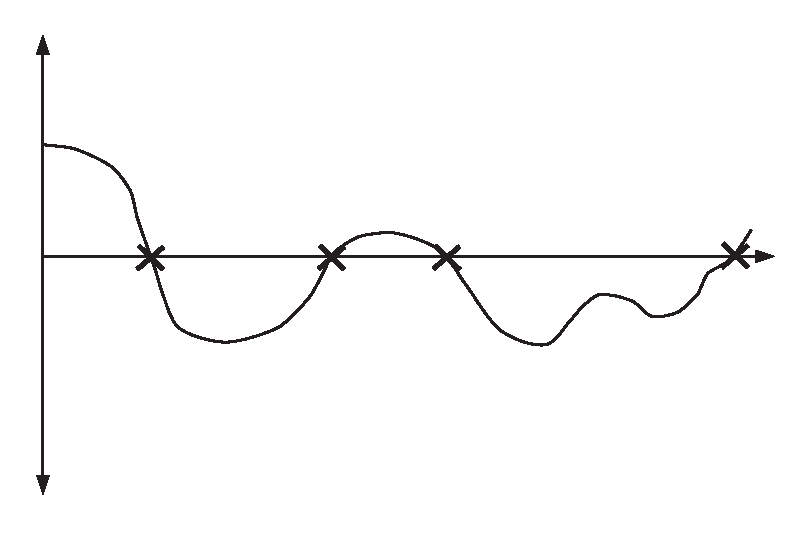
\includegraphics[scale=1.0]{Images/EventsFunction.eps}
   % \end{picture}
    \caption{ Sample Event Function Output }
    \label{fig:SampleEventFunction}
\end{figure*}

\begin{equation}
    \mathbf{F} = \mathbf{F} (t, \mathbf{x}(t),\mathbf{C}   )
\end{equation}
%
We want to find all $t$ such that
%
\begin{equation}
    \mathbf{F} (t, \mathbf{x}(t),\mathbf{C}   ) = 0
\end{equation}


\section{Root Finding Options in GMAT}

In implementing a root finding approach, we need to balance accuracy
and the need to find every root, with speed and performance.  One
way to do this is to allow the user to select between different
approaches depending upon the accuracy needed for a particular
application.   The user has several controls to tell GMAT how to
determine if a zero crossing has occurred, and how to calculate the
numerical value of a root if one has been detected. Let's look at
the choices implemented in GMAT, and discuss some options that can
be included if a more robust method is required.

The first group of controls available to the user are related to how
or if GMAT tries to determine if a root has occurred.  The user can
provide a flag in the output of an Event Function that tells GMAT
whether it is possible that a root has occurred during the last
integration step. This flag is notated as $\mathbf{p}$ and is
discussed in section \ref{sec:EventFunctionMathDef}.  If an element
of $\mathbf{p}$ is zero, then GMAT will not use more sophisticated
and therefore more computationally intensive methods to determine if
a zero crossing for the particular component of the event function
has occurred.  $\mathbf{p}$ can be either zero or one, and can
change value during propagation.  If $\mathbf{p}$ changes from zero
to one, GMAT begins using a root checking method specified by the
user to determine if a zero crossing has occurred, and begins
storing function data  in case it is needed to interpolate a root
location.

The second control that determines if a  zero crossing has occurred
is called \st{RootCheckMethod} in the GMAT script language.  There
are several RootCheckMethod options available and the user can
currently select between \st{FunctionSignChange} and
\st{PolynomialFit}.  If the user selects \st{FunctionSignChange},
then GMAT looks for sign changes in the function output to determine
if a zero crossing has occurred.  If the user selects
\st{PolynomialFit}, then GMAT fits a polynomial to the Event
Function data, and checks to see if the polynomial has any real
roots. If the polynomial has real roots, then a zero crossing has
occurred. The type of polynomial GMAT uses in \st{RootCheckMethod}
is the same as it uses in \st{RootFindingMethod} and is discussed in
more detail below.

If a zero crossing is detected, there are many ways to determine the
numerical value of the root.  The user can select between the
different methods by using the \st{RootSolvingMethod} option. The
two methods currently implemented in GMAT are called
\st{QuadraticPolynomial} and \st{CubicSpline} in the GMAT script
language.  As the name suggests, if the user selects
\st{QuadraticPolynomial}, then GMAT uses the last three function
values to create a quadratic polynomial.  Then, the quadratic
equation is used to determine the root locations. Similarly, if the
user selects \st{CubicSpline}, GMAT constructs a cubic spline and
then uses interpolation to find the root value.

Allowing the options above requires that care is taken in designing
an algorithm to track events.  In the next section we discuss some
of the issues that must be addressed in the Event Function
algorithm, and present a flow chart that describes the algorithm in
detail

\section{Algorithm for Event Functions }


\begin{table}[htb]
\caption{ Variables in Event Function Algorithm}
\begin{tabular}{p{.5 in} p{2.5 in}}
   \hline
   Variable & Definition\\
   \hline \hline
    $n_r$     & Number of data points required to use the requested \st{RootSolvingMethod} option \\
    $n_c$     & Number of data points required to use the requested \st{RootCheckMethod} option\\
    $\mathbf{f}$  & A vector of function values provided by the user
    defined Event Function\\
    $N$           &  The length of $\mathbf{f}$, which is the number
    function values contained in  the output of a user defined Event
    Function.\\
    $\mathbf{d}$   &  A vector of flags (length $N$) that defines which
    type of roots to track.  (negative to positive, positive to
    negative, or both)\\
    $\mathbf{p}$   &  A vector of flags (length $N$) that tells whether or not a
    zero crossing is possible.  A component of $\mathbf{p}$ is one
    if a root is possible, otherwise it is zero.\\
    $\mathbf{Startup}$ & A vector of flags of lenght $N$.  The components of $\mathbf{Startup}$ correspond to the components of $\mathbf{f}$.
                        A component of $\mathbf{Startup}$ is one, if there is
                       less than max($n_r$,$n_c$) data points saved for use in root finding.
                        Otherwise, a component of $\mathbf{Startup}$ is zero.\\
   \hline
 \end{tabular}
 \label{Table:VariablesinEventFunctionChart}
\end{table}



\clearpage
\begin{figure*}[htb]
    \centering
    \begin{picture}(0,400)(310,300)
        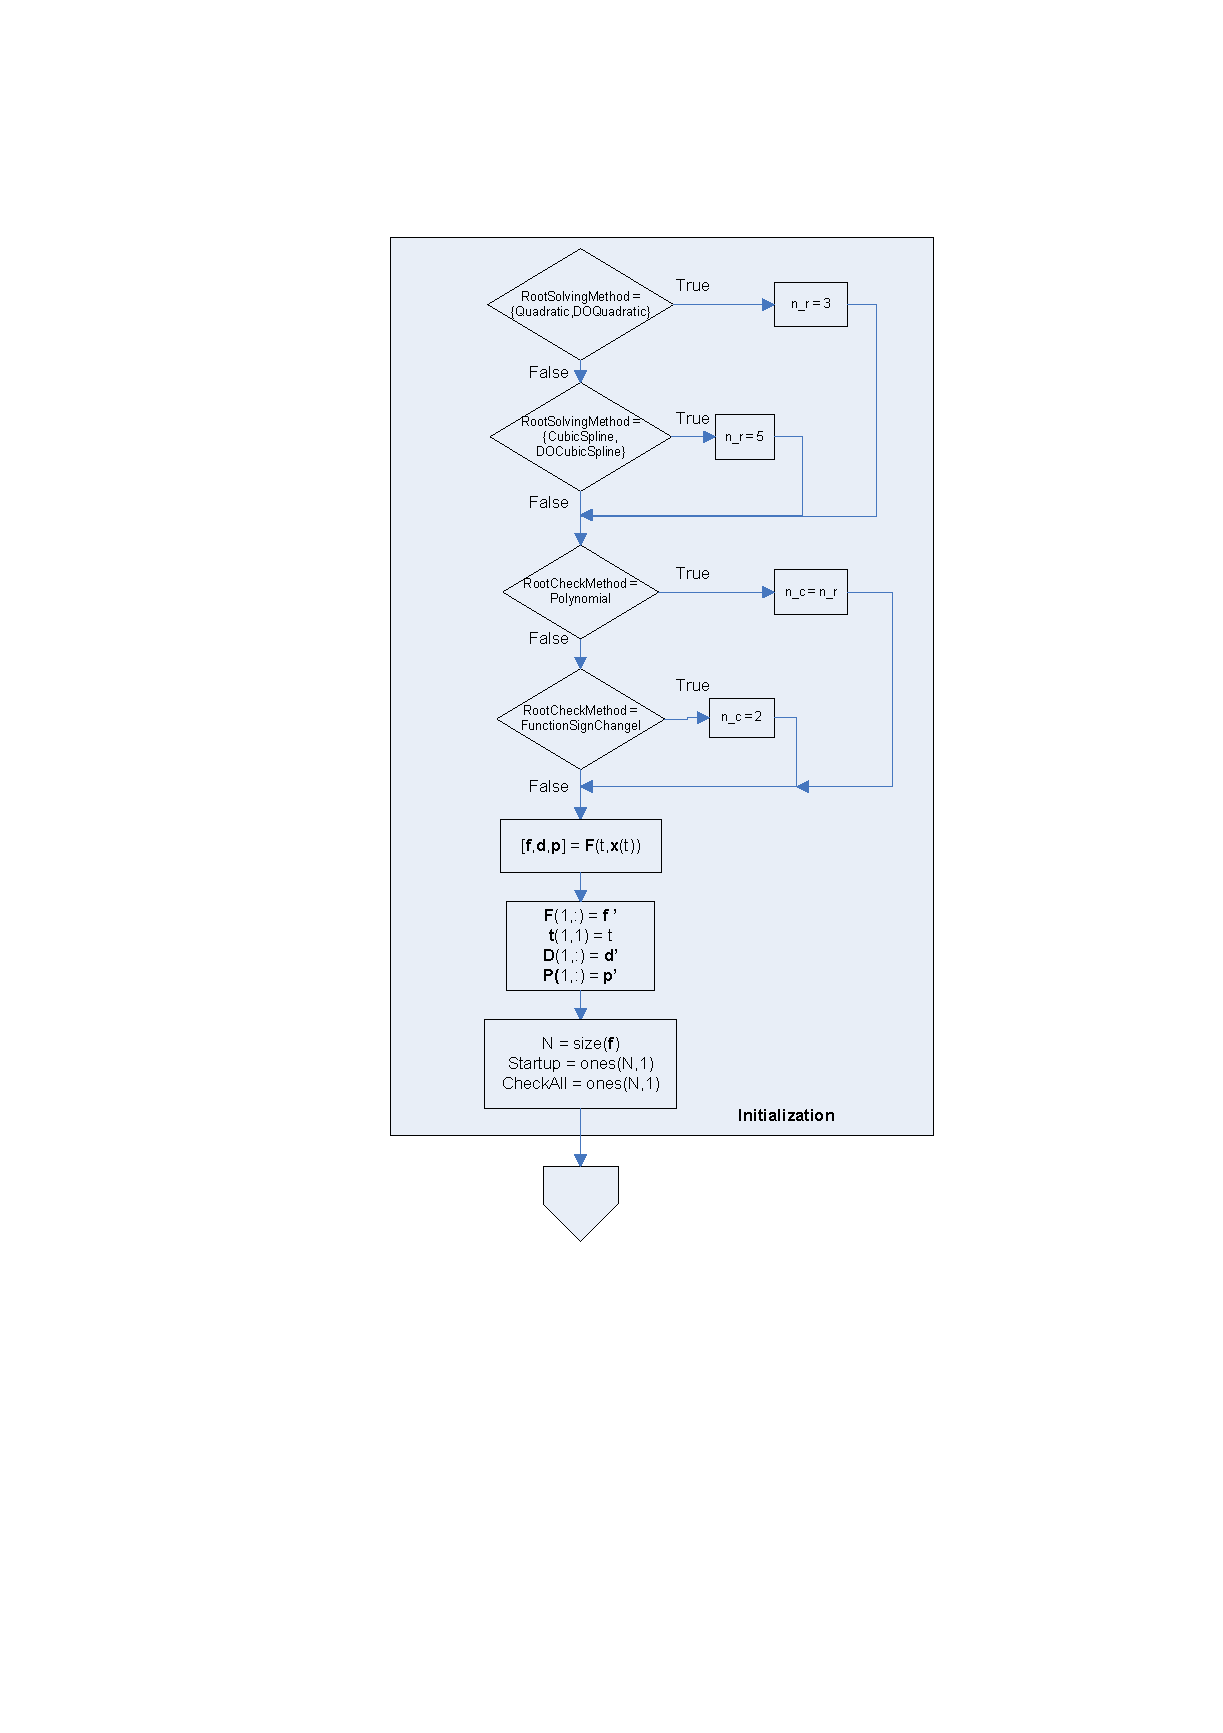
\includegraphics[scale = 1.0]{Images/EventFunctionsFlowChart.eps}
    \end{picture}
    \vspace{1 in}
    \caption{ Initializations for the Event Location Algorithm }
    \label{Plot:EventFunctionsFlowChart}
\end{figure*}

\clearpage
\begin{figure*}[htb]
    \centering
    \begin{picture}(0,400)(265,210)
        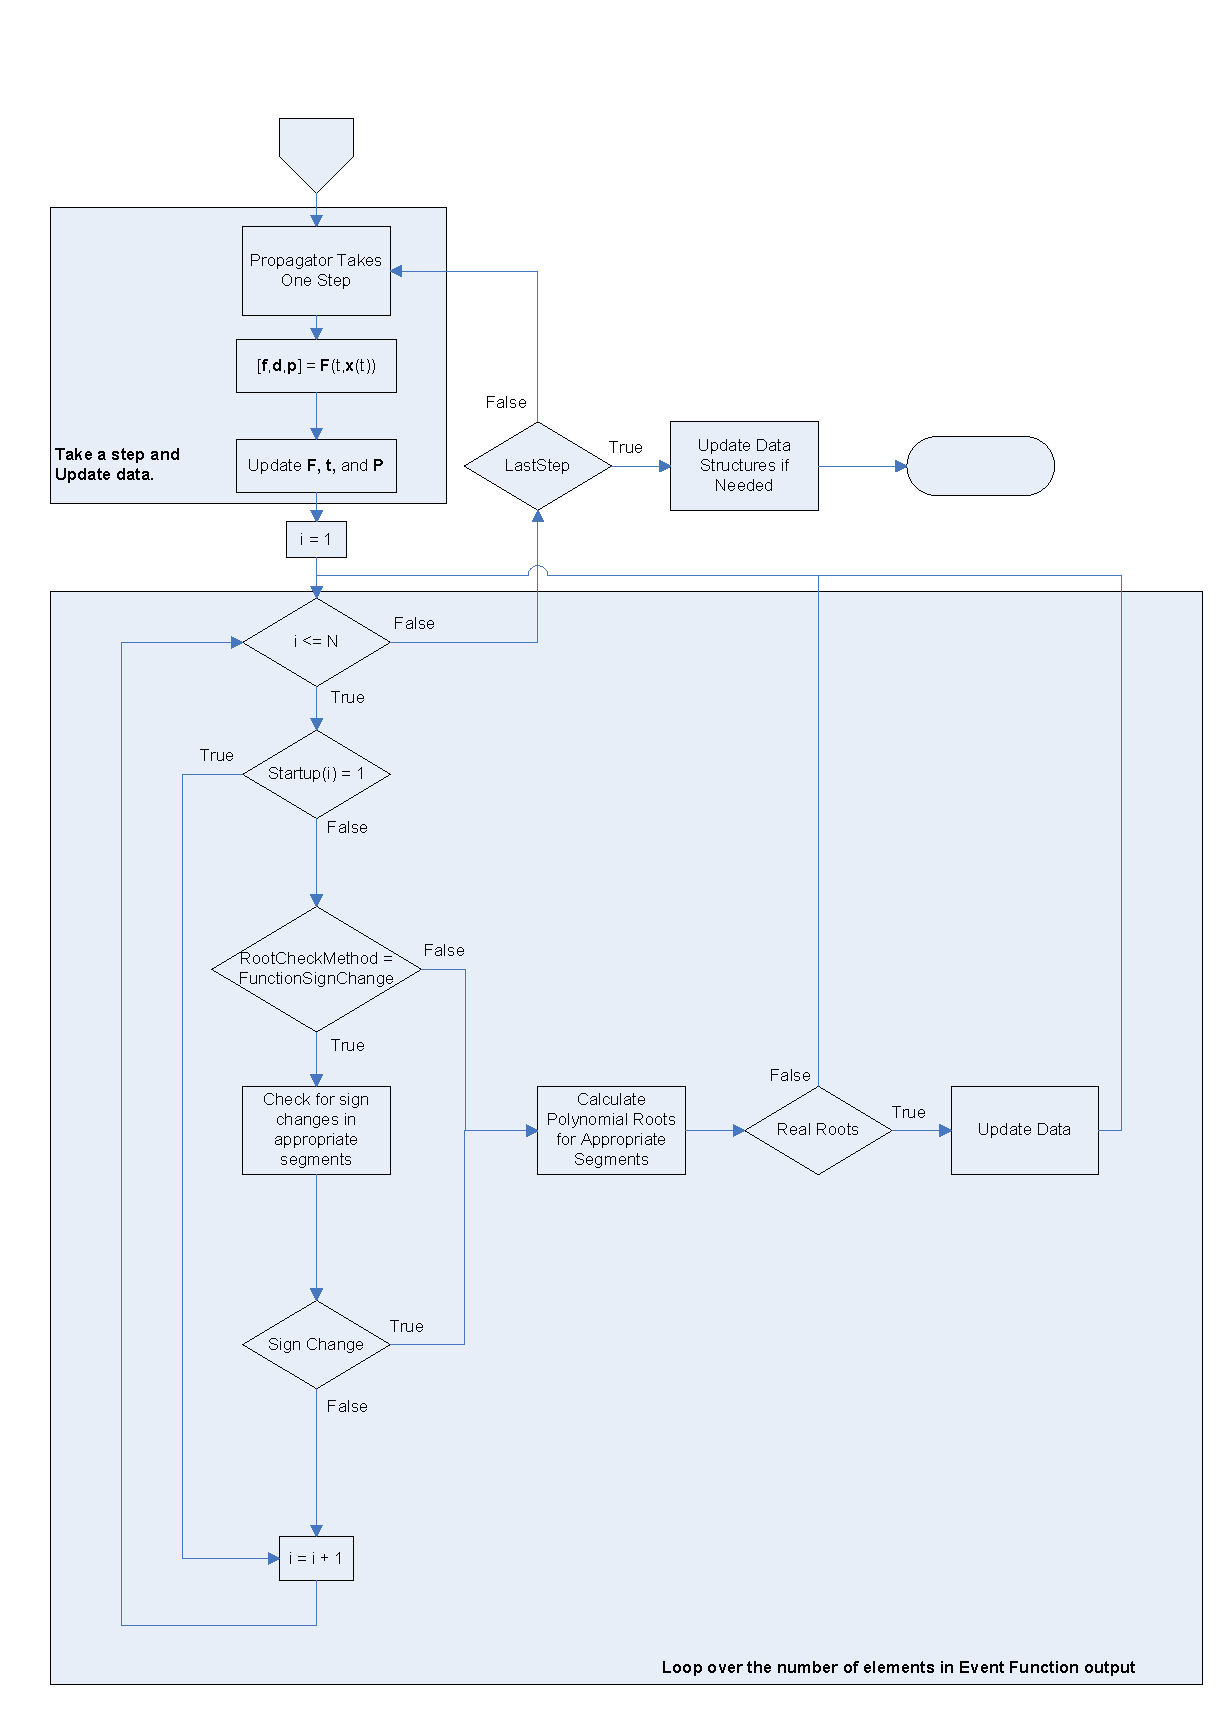
\includegraphics[scale = .9]{Images/EventFunctionsFlowChart2.eps}
    \end{picture}
    \vspace{1 in}
    \caption{ Event Location Algorithm }
    \label{Plot:EventFunctionsFlowChart2}
\end{figure*}

\clearpage


\section{Appendix 1:  Root Finding Algorithms}

\section{Quadratic Polynomial }


We are given three data points defined by a vector of independent
variables
%
\begin{equation}
     \mathbf{x} = [\hspace{.05 in} x_1 \hspace{.05 in} x_2 \hspace{.05 in}
     x_3 \hspace{.05
     in}]^T
\end{equation}
%
and a vector of corresponding dependent variables
%
\begin{equation}
     \mathbf{y} = [\hspace{.05 in} y_1 \hspace{.05 in} y_2 \hspace{.05 in}
     y_3  \hspace{.05
     in}]^T
\end{equation}
%
we wish to find a quadratic polynomial that fits the data such
that
%
\begin{equation}
   y = Ax^2 + Bx +C
\end{equation}
%
We begin by forming the system of linear equations
%
\begin{equation}
    \left(%
    \begin{array}{ccc}
       x_1^2 & x_1 & 1 \\
       x_2^2 & x_2 & 1 \\
       x_3^2 & x_3 & 1 \\
    \end{array}%
    \right)
    %
     \left(%
    \begin{array}{ccc}
       A \\
       B \\
       C \\
    \end{array}%
    \right)
    =
     \left(%
    \begin{array}{ccc}
       y_1 \\
       y_2 \\
       y_3 \\
    \end{array}%
    \right)
\end{equation}
%
We can solve for the coefficients using
%
\begin{equation}
    A = \frac{
    %  Numerator
    \left|%
    \begin{array}{ccc}
       y_1 & x_1 & 1 \\
       y_2 & x_2 & 1 \\
       y_3 & x_3 & 1 \\
    \end{array}%
    \right|
    }
    %  Denominator
    {    \left|%
    \begin{array}{ccc}
       x_1^2 & x_1 & 1 \\
       x_2^2 & x_2 & 1 \\
       x_3^2 & x_3 & 1 \\
    \end{array}%
    \right|}
\end{equation}
%
\begin{equation}
    B = \frac{
    %  Numerator
    \left|%
    \begin{array}{ccc}
     x_1^2 & y_1 & 1 \\
     x_2^2 & y_2 & 1 \\
     x_3^2 & y_3 & 1 \\
    \end{array}%
    \right|
    }
    %  Denominator
    {    \left|%
    \begin{array}{ccc}
       x_1^2 & x_1 & 1 \\
       x_2^2 & x_2 & 1 \\
       x_3^2 & x_3 & 1 \\
    \end{array}%
    \right|}
\end{equation}
%
\begin{equation}
    C = y_3 - A x_3^2 - B x_3
\end{equation}

\section{Cubic Spline (Not-a-Knot) }

We are given five data points defined by a vector of independent
variables
%
\begin{equation}
     \mathbf{x} = [\hspace{.05 in} x_1 \hspace{.05 in} x_2 \hspace{.05 in}
     x_3 \hspace{.05 in} x_4 \hspace{.05 in} x_5 \hspace{.05
     in}]^T
\end{equation}
%
and a vector of corresponding dependent variables
%
\begin{equation}
     \mathbf{y} = [\hspace{.05 in} y_1 \hspace{.05 in} y_2 \hspace{.05 in}
     y_3 \hspace{.05 in} y_4 \hspace{.05 in} y_5 \hspace{.05
     in}]^T
\end{equation}
%
we wish to find the four cubic polynomials, $i = 1,2,3,4$, such
that
%
\begin{equation}
    p_i = a_i(x - x_i)^3 + b_i(x - x_i)^2 + c_i(x - x_i) + d_i
\end{equation}
%
where the values for $x_i$ are known from the inputs.

To calculate the coefficients $a_i$, $b_i$, $c_i$, and $d_i$ we
start by calculating the eight quantities
%
\begin{eqnarray}
     h_i      &=& x_{i+1} - x_i\\
     \Delta_i &=& \displaystyle\frac{y_{i+1} - y_i}{h_i}
\end{eqnarray}
%
Next we solve the following system of linear equations
%
\begin{equation}
     \mathbf{A}\mathbf{S} = \mathbf{B}
\end{equation}
%
where the components of $\mathbf{A}$ are given by
%
\begin{eqnarray}
     A_{11} &=& 2h_2 + h_1 \\
     A_{12} &=& 2h_1 + h_2 \\
     A_{13} &=& 0 \\
     A_{21} &=& 0 \\
     A_{22} &=& h_3 + 2h_4 \\
     A_{23} &=& 2h_3 + h_4 \\
     A_{31} &=& \displaystyle\frac{h_2^2}{h_1 + h_2} \\
     A_{32} &=& \displaystyle\frac{h_1h_2}{( h_1 + h_2 )} + 2( h_2 + h_3 ) + \displaystyle\frac{h_3h_4}{( h_3 + h_4
     )}\\
     A_{33} &=& \displaystyle\frac{h_3^2}{h_3 + h_4}
\end{eqnarray}
%
the components of $\mathbf{B}$ are
%
\begin{eqnarray}
    B_{11} &=& 6( \Delta_2 - \Delta_1 )\\
    B_{21} &=& 6( \Delta_4 - \Delta_3 )\\
    B_{31} &=& 6( \Delta_3 - \Delta_2 )
\end{eqnarray}
%
and $\mathbf{S} = [\hspace{.05 in} S_1 \hspace{.05 in} S_3
\hspace{.05 in} S_5 \hspace{.05 in}]^T$. We can solve for the
components of $\mathbf{S}$ using Cramer's Rule as follows
%
\begin{equation}
    S_1 = \frac{
    %  Numerator
    \left|%
    \begin{array}{ccc}
       B_{11} & A_{12} & A_{13} \\
       B_{21} & A_{22} & A_{23} \\
       B_{31} & A_{32} & A_{33} \\
    \end{array}%
    \right|
    }
    %  Denominator
    {\mathbf{| \mathbf{A}|}}
\end{equation}
%
\begin{equation}
    S_3 = \frac{
    %  Numerator
    \left|%
    \begin{array}{ccc}
       A_{11} & B_{11} & A_{13} \\
       A_{21} & B_{21} & A_{23} \\
       A_{31} & B_{31} & A_{33} \\
    \end{array}%
    \right|
    }
    %  Denominator
    {\mathbf{| \mathbf{A}|}}
\end{equation}
%
\begin{equation}
     S_5 = \frac{B_{31} - A_{31} S_1 - A_{32} S_3}{A_{33}}
\end{equation}
%
Now we can calculate $S_2$ and $S_4$ using
%
\begin{equation}
     S_2 = \frac{ h_2 S_1 + h_1 S_3  }{  h_1 + h_2 };
\end{equation}
%
\begin{equation}
     S_4 = \frac{ h_4 S_3 + h_3 S_5  }{  h_3 + h_4 };
\end{equation}
%

Finally, the coefficients for the $i^{th}$ cubic polynomial are
given by
\begin{eqnarray}
   a_i &=&  \frac{ S_{i+1} - S_i   }{ 6  h_i}\\
   b_i &=&  \frac{S_i}{2}\\
   c_i &=&  \frac{ y_{i+1} - y_i  }{ h_i } - \frac{ 2 h_i S_i + h_i S_{i+1} }{  6
   }\\
   d_i &=&  y_i
\end{eqnarray}

\chapter{Graphics} \label{Ch:Graphics}

\section{Ground Track Plotting}

A ground track plot displays spherical latitude and longitude over a Poincare (unwrapped cylinder) projection of a body's surface geography. The algormithm used to generate a ground track plot ensures that line wrapping at the plot boundaries is handled correctly, and that when wrapping occurs, the plot is interpolated to the plot boundary.

Longitude is computed by converting position and velocity of the object to the body fixed system of the ground track plot central body.  Define $x$, $y$, and $z$ as the body fixed coordinates of the object.   The longitude is calculated using
%
\begin{equation}
     \lambda =  atan2(y,x)
\end{equation}
%
and the latitude is calculate using
%
\begin{equation}
     \phi = asin{\frac{z}{r}}
\end{equation}
%
where
%
\begin{equation}
    r = \sqrt{x^2 + y^2 + z^2}
\end{equation}

There are three special cases to consider when plotting a new point on a ground track: (1) the new point wraps off the right-hand side of the plot, (2) the new point wraps off the left-had side of the plot, and (3) the new point does not wrap off either plot boundary.  When wrapping oocurs as in cases (1) and (2), the plot algorithm must perform  "Pen Up" and "Pen Down" commands to avoid connecting points on opposite ends of the plot with a spurious straight line.  Secondly, when wrapping occurs, the system must interpolate the line segments to plot boundaries. 

The test to determine the case depends  upon whether the object is moving clockwise or counterclockwise in the body fixed system of the ground track plot central body.    The orbit direction is determined by evaluating the z component of orbit angular momentum expressed in the body fixed system.  Define a variable $d$ that is positive for clockwise motion in the body fixed system (the spacecraft is moving to the right on a ground track plot), and negative for counterclockwise motion. (spacecraft is moving to the left on  a ground track plot), and 0 for no motion.   The variable $d$ is computed as follows
%
\begin{equation}
   d = sign(x \dot{y} - \dot{x}y)
\end{equation}
%
%
\begin{equation}
    m = \frac{\phi_i -\phi_{i-1}}{\lambda_i - \lambda_{i-1}}
\end{equation}

\begin{center}
\begin{minipage}{6 in}
\begin{small}
\begin{algorithm}[H]

    \KwIn{$\lambda_i,\lambda_{i-1},\phi_i,\phi_{i-1},d_i,d_{i-1}$}
    %
    \KwOut{Updated Ground Track Plot}
    $m\lambda_i^+ = mod(\lambda_i,2 \pi)$\;
    $m\lambda_{i-1}^+ = mod(\lambda_{i-1},2 \pi)$\;
    $m\lambda_i^- = mod(\lambda_i,-2 \pi)$\;
    $m\lambda_{i-1}^- = mod(\lambda_{i-1},-2 \pi)$\;
\% New point wraps off RHS border\;
  \uIf{ $ d_i = d_{i-1} = 1 $ \mbox{And} $m\lambda_{i-1}^+ < \pi $ \mbox{And} $m\lambda_i^+ > \pi$}
          {
           
           $m = \displaystyle\frac{\phi_i - \phi_{i-1}}{m\lambda_i^+ - m\lambda_{i-1}^+}$\;
           $\phi_b = m (\pi - m\lambda_i^+) + \phi_i$\;
           Plot line segment from ($\lambda_{i-1},\phi_{i-1}$) to ($\pi,\phi_b$)\;
           Plot line segment from ($-\pi,\phi_b$) to ($\lambda_i,\phi_i$)\;
          }{
          \% New point wraps off LHS border\;
  \uElseIf {$ d_i = d_{i-1} = -1 $ \mbox{And} $m\lambda_i^- < -\pi $ \mbox{And} $m\lambda_{i-1}^- > -\pi$}
              {
           
           $m = \displaystyle\frac{\phi_i - \phi_{i-1}}{m\lambda_i^- - m\lambda_{i-1}^- }$\;
           $\phi_b = m (-\pi - m\lambda_i^-) + \phi_i$\;
           Plot line segment from ($\lambda_{i-1},\phi_{i-1}$) to ($-\pi,\phi_b$)\;
           Plot line segment from ($\pi,\phi_b$) to ($\lambda_i,\phi_i$)\;
               }
               \% New does not wrap off plot border \;
  \Else 
           {
                Plot line segment from ($\lambda_{i-1},\phi_{i-1}$) to ($\lambda_i,\phi_i$)\;
            }
    }    
    \hspace{.2 in}
    %
    \label{alg:GroundTrackAlgorithm}\caption{Algorithm for Updating A Ground Track Plot}
    %
\end{algorithm}
\end{small}
\end{minipage}
\end{center}

\section{Footprint and Limb Computation}

\subsection{Overview}

Computing an instrument footprint or the Earth Limb as viewed from a spacecraft involves essentially three related problems: (1) Determining the intersection of a given line with a given ellipsoid, (2) determination of a line tangent to a known ellipsoid, and (3) determining how to select the points along the footprint or limb curve to provide a smooth plot in the graphics.    These problems are related and discussed in order below starting with the problem of computing the intersection of a line and an ellipsoid.

\subsection{Intersection of Line and Ellipsoid}

Begin by defining a ray $\boldsymbol{\ell}$ such that
%
\begin{equation}
    \boldsymbol{\ell} = \mathbf{p} + \alpha\hat{\mathbf{d}} \label{Eq:RayParametrization}
\end{equation}
%
where $\mathbf{p}$ (in this context the usually location of a spacecraft) is the the starting location of ray $\boldsymbol{\ell}$, $\hat{\mathbf{d}}$ is the unit vector in the direction of the ray, and $\alpha$ is the distance from coordinates $\mathbf{p}$ in the direction.  The equation for a tri-axial ellipoid is defined as
%
\begin{equation}
  \frac{x^2}{R_x^2} + \frac{y^2}{R_y^2} + \frac{z^2}{R_z^2} - 1 = 0 \label{Eq:TriAxialEllipsoid}
\end{equation}
%
where $R_x$, $R_y$, and $R_z$ are the ellipsoid radii in the $x$, $y$, and $z$ directions respectively.
For simplicity of notation, we'll assume all coordinates such $x$, $y$, and $z$, and ray $\boldsymbol\ell$ are 
expressed in the body coordinates of the ellipsoid.
%
Subtituting Eq.~(\ref{Eq:RayParametrization}) into Eq.~(\ref{Eq:TriAxialEllipsoid}) results in
%
\begin{equation}
    \frac{\boldsymbol{\ell}^T \hat{\mathbf{i}}}{R_x^2} + \frac{\boldsymbol{\ell}^T \hat{\mathbf{j}}}{R_y^2} 
    + \frac{\boldsymbol{\ell}^T \hat{\mathbf{k}}}{R_z^2} - 1 = 0 \label{Eq:EllipseSimltaneous}
\end{equation}
%
where $\hat{\mathbf{i}}$, $\hat{\mathbf{i}}$, and $\hat{\mathbf{i}}$ are unit vectors in the $x$, $y$, and $z$ directions respectively.  Define $\alpha^*$ as the value of $\alpha$ that simulteoulsy satisfies both the equation for ray $\boldsymbol{\ell}$ and the equation for the triaxial ellipoid.  Expanding Eq.~(\ref{Eq:EllipseSimltaneous}) and grouping terms by powers of $\alpha^*$ yields
%
\begin{equation}
    \alpha^{*2}\left( \frac{d_x^2}{R_x^2} + \frac{d_y^2}{R_y^2} + \frac{d_z^2}{R_z^2} \right) +
    2\alpha^{*}\left( \frac{d_x p_x}{R_x^2} + \frac{d_y p_y}{R_y^2} + \frac{d_z p_z}{R_z^2} \right)+
    \left( \frac{p_x^2}{R_x^2} + \frac{p_y^2}{R_y^2} + \frac{p_z^2}{R_z^2} - 1\right) = 0
\end{equation}
%
This is a quadratic equation and the solution is 
%
\begin{equation}
    \alpha^* = \frac{-B \pm \sqrt{B^2 - 4 A C}}{2A}\label{Eq:Quadratic}
\end{equation}
%
where 
%
\begin{eqnarray}
    A &=& \left( \frac{d_x^2}{R_x^2} + \frac{d_y^2}{R_y^2} + \frac{d_z^2}{R_z^2} \right)\\
    B &=& 2\left( \frac{d_x p_x}{R_x^2} + \frac{d_y p_y}{R_y^2} + \frac{d_z p_z}{R_z^2} \right)\\
    C &=& \left( \frac{p_x^2}{R_x^2} + \frac{p_y^2}{R_y^2} + \frac{p_z^2}{R_z^2} - 1\right) 
\end{eqnarray}
%
There are three physical types of solutions for $\alpha^*$ given by Eq.~(\ref{Eq:Quadratic}).  If $(B^2 - 4 A C) < 0$ then ray $\boldsymbol\ell$ does not intersect
the ellipoid.  If $(B^2 - 4 A C) = 0$ then ray $\boldsymbol\ell$ is tangent to the ellipsoid (we'll revisit this relation when computing the limb curve). In this case,
%
\begin{equation}
    \boldsymbol{\ell}^* = \mathbf{p} -\frac{B}{2A}\hat{\mathbf{d}} 
\end{equation}
%
Finally, if $(B^2 - 4 A C) > 0$ then ray $\boldsymbol\ell$ intersects the ellipsoid
at two locations.  For graphics purposes, we require the smaller value of $\alpha^*$ given by Eq.~(\ref{Eq:Quadratic}). If we define $\boldsymbol\alpha^*$ as a vector containing the two solutions for $\alpha$ corresponding to the two intersection points, then, the equation for the nearest intersection point, $\boldsymbol{\ell}^*$ is given by
%
\begin{equation}
    \boldsymbol{\ell}^* = \mathbf{p} + min(\boldsymbol\alpha^*)\hat{\mathbf{d}} 
\end{equation}

\subsection{Determining the Limb Region}

\subsection{Selecting Points for Accurate Graphics}
\chapter{Numerical Algorithms} \label{Ch:NumericalAlgorithms}

\section{Lagrange Interpolation}

Below we describe the algorithm used for lagrange interpolation.
This includes specifying how points  from the known data are chosen
for interpolation, and how interpolation is performed for multiple
function values (i.e. position and velocity) at the desired
interpolation point.

Assume we have $m$ functions to interpolate and that each function
is known at $\ell$ values of the independent variable $x$ (in
ephemeris interpolation this is time) as illustrated in
Table~\ref{Table:InterpolationData}. Given some point, say $x'$, we
desire the interpolated values of the functions, or $\mathbf{f}'
\approx \mathbf{P}(x')$ where $P$ is the Lagrange interpolating
polynomial.

%
\begin{table}[ht] \centering
\caption{Example of Data for interpolation}
 \begin{tabular}{ccccc}  \hline \hline
         x & $\mathbf{f}_1$ & $\mathbf{f}_2$ & \dots & $\mathbf{f}_m$ \\ \hline
         $x_1$ & $f_1(x_1)$ &  $f_2(x_1)$ &  \dots & $f_m(x_1)$\\
         $x_2$ & $f_1(x_2)$ &  $f_2(x_2)$ &  \dots &$f_m(x_2)$\\
         $x_3$ & $f_1(x_3)$ &  $f_2(x_3)$ &  \dots &$f_m(x_3)$\\
         $x_4$ & $f_1(x_4)$ &  $f_2(x_4)$ &  \dots &$f_m(x_4)$\\
         \vdots   & \vdots &   \vdots &  $\ddots$ & \vdots\\
         $x_{\ell-1}$ & $f_1(x_{\ell-1})$ &  $f_2(x_{\ell-1})$ & \dots & $f_m(x_{\ell-1})$\\
         $x_{\ell}$ & $f_1(x_\ell)$ &  $f_2(x_\ell)$ & \dots & $f_m(x_\ell)$\\
         \hline \hline
         \label{Table:InterpolationData}
 \end{tabular}
 \end{table}
 %

Before proceeding we define the following variables:
%
\begin{center}
    \begin{minipage}[t]{5.0 in}
        \begin{tabbing}[htbp!]
            123456 \= dummy line \kill
            $\mathbf{x}$ \> $m_x$ x 1 Known values of the independent variable (monotonically increasing or decreasing) \\
            $x'$ \>  Value of independent variable a the required interpolation point\\
            $\mathbf{f}_i$ \> $m_x$ x $m_f$ Array of dependent variable values for the $i^{th}$ function\\
            $\mathbf{f}'$ \> 1 x $m_f$ Array of interpolated function values at $x'$\\
            $n$ \> Order of interpolation \\
            $m_x$  \>  Number of points in $\mathbf{x}$ and $\mathbf{f}_i$ \\
            $m_f$  \>  Number of functions to be interpolated \\
        \end{tabbing}
    \end{minipage}
\end{center}

For interpolation to be feasible, several conditions must be
satisfied.  First, $x'$ must lie between the minimum and maximum
value of $\mathbf{x}$, or at the boundaries ( otherwise we would be
extrapolating ):
%
\begin{equation}
     x' \geq \mbox{min}(\mathbf{x})
\end{equation}
%
and
%
\begin{equation}
     x' \leq \mbox{max}(\mathbf{x})
\end{equation}
%
Second, there must be enough data points in points in $\mathbf{x}$
to support interpolation to the desired order.  If the requested
interpolation is of order $n$, then we require $n+1$ data points to
perform the interpolation.  Hence the following criteria must be
met:
%
\begin{equation}
    m_x \geq n + 1
\end{equation}
%

If the requested interpolation is feasible, we must choose the
subset of $\mathbf{x}$ to use for interpolating the data at $x'$.
Define $x(q)$ as the $q^{th}$ element of $\mathbf{x}$. Given $x'$,
we choose $q$ to minimize the difference between $x'$ and the mean
of $x(q)$ and $x(q + n)$, or:
%
\begin{equation}
    \underset{q}{\mbox{min }} \left| \frac{x(q+n) + x(q)}{2} - x'\right|  \hspace{.3 in} ( q \in 1,2,3,... m_x)
\end{equation}
%
Choosing $q$ in this way places $x'$ as near to the center of the
interpolation interval as possible.

The standard formula for the Lagrange interpolating polynomial for a
single function is
%
\begin{equation}
    P(x) =  \sum_{k=1}^n P_j(x) \label{Eq:LagrangeInterp}
\end{equation}
%
where $P_j(x)$ is given by
%
\begin{equation}
   P_j(x) = y_j\prod_{k=1,k \neq j}^n\frac{x - x_j}{x_j - x_k} \label{Eq:LagrangePj}
\end{equation}
%
Lagrange interpolation is an efficient method when interpolating
multiple data sets available at the same independent variable
points.  This is due to the fact that the product term in
Eq.~(\ref{Eq:LagrangePj}) is only a function of the values of the
independent variables and the desired interpolation point and not on
the function being interpolated.  As a result, we can evaluate the
product term one time and use it for many functions (which is what
is done when interpolating an ephemeris file).  The algorithm for
implementing Lagrangian interpolation for multiple functions is
shown below.

\begin{center}
\begin{minipage}{6 in}
\begin{small}
\begin{algorithm}[H]

    \SetLine \KwIn{$\mathbf{x}, \mathbf{f},x',q,n$}
    %
    \KwOut{$\mathbf{f}'$}
    %
    $\mathbf{f}' = \mathbf{0}_{(1 \mbox{ x } m_f)}$\;
    %
    \For{ i = q to $q+n$}
    {
        $\mathbf{prod} = f(i,:)$ \% The $i^{th}$ row of $\mathbf{f}$ \;
        \For{ $j = q$ to $q+n$}
        {
            \If{ $ i \neq j$}
            {
            \% The product in Eq.~(\ref{Eq:LagrangePj})\;
                    $ \mathbf{prod} = \mathbf{prod} \cdot \displaystyle\frac{x' - x(j)}{x(i) - x(j)}$\;
            }
        }
       \% The summation in Eq.~(\ref{Eq:LagrangeInterp})\;
       $ \mathbf{f}'= \mathbf{f}' + \mathbf{prod}$\;
    }
    \hspace{.2 in}
    %
    \label{alg:LagrangeInterpolation}\caption{Algorithm for Lagrangian Interpolation}
    %
\end{algorithm}
\end{small}
\end{minipage}
\end{center}


\section{Quadratic Polynomial Interpolation }


We are given three data points defined by a vector of independent
variables
%
\begin{equation}
     \mathbf{x} = [\hspace{.05 in} x_1 \hspace{.05 in} x_2 \hspace{.05 in}
     x_3 \hspace{.05
     in}]^T
\end{equation}
%
and a vector of corresponding dependent variables
%
\begin{equation}
     \mathbf{y} = [\hspace{.05 in} y_1 \hspace{.05 in} y_2 \hspace{.05 in}
     y_3  \hspace{.05
     in}]^T
\end{equation}
%
we wish to find a quadratic polynomial that fits the data such that
%
\begin{equation}
   y = Ax^2 + Bx +C
\end{equation}
%
We begin by forming the system of linear equations
%
\begin{equation}
    \left(%
    \begin{array}{ccc}
       x_1^2 & x_1 & 1 \\
       x_2^2 & x_2 & 1 \\
       x_3^2 & x_3 & 1 \\
    \end{array}%
    \right)
    %
     \left(%
    \begin{array}{ccc}
       A \\
       B \\
       C \\
    \end{array}%
    \right)
    =
     \left(%
    \begin{array}{ccc}
       y_1 \\
       y_2 \\
       y_3 \\
    \end{array}%
    \right)
\end{equation}
%
We can solve for the coefficients using
%
\begin{equation}
    A = \frac{
    %  Numerator
    \left|%
    \begin{array}{ccc}
       y_1 & x_1 & 1 \\
       y_2 & x_2 & 1 \\
       y_3 & x_3 & 1 \\
    \end{array}%
    \right|
    }
    %  Denominator
    {    \left|%
    \begin{array}{ccc}
       x_1^2 & x_1 & 1 \\
       x_2^2 & x_2 & 1 \\
       x_3^2 & x_3 & 1 \\
    \end{array}%
    \right|}
\end{equation}
%
\begin{equation}
    B = \frac{
    %  Numerator
    \left|%
    \begin{array}{ccc}
     x_1^2 & y_1 & 1 \\
     x_2^2 & y_2 & 1 \\
     x_3^2 & y_3 & 1 \\
    \end{array}%
    \right|
    }
    %  Denominator
    {    \left|%
    \begin{array}{ccc}
       x_1^2 & x_1 & 1 \\
       x_2^2 & x_2 & 1 \\
       x_3^2 & x_3 & 1 \\
    \end{array}%
    \right|}
\end{equation}
%
\begin{equation}
    C = y_3 - A x_3^2 - B x_3
\end{equation}

\section{Cubic Spline (Not-a-Knot) Interpolation }

We are given five data points defined by a vector of independent
variables
%
\begin{equation}
     \mathbf{x} = [\hspace{.05 in} x_1 \hspace{.05 in} x_2 \hspace{.05 in}
     x_3 \hspace{.05 in} x_4 \hspace{.05 in} x_5 \hspace{.05
     in}]^T
\end{equation}
%
and a vector of corresponding dependent variables
%
\begin{equation}
     \mathbf{y} = [\hspace{.05 in} y_1 \hspace{.05 in} y_2 \hspace{.05 in}
     y_3 \hspace{.05 in} y_4 \hspace{.05 in} y_5 \hspace{.05
     in}]^T
\end{equation}
%
we wish to find the four cubic polynomials, $i = 1,2,3,4$, such that
%
\begin{equation}
    p_i = a_i(x - x_i)^3 + b_i(x - x_i)^2 + c_i(x - x_i) + d_i
\end{equation}
%
where the values for $x_i$ are known from the inputs.

To calculate the coefficients $a_i$, $b_i$, $c_i$, and $d_i$ we
start by calculating the eight quantities
%
\begin{eqnarray}
     h_i      &=& x_{i+1} - x_i\\
     \Delta_i &=& \displaystyle\frac{y_{i+1} - y_i}{h_i}
\end{eqnarray}
%
Next we solve the following system of linear equations
%
\begin{equation}
     \mathbf{A}\mathbf{S} = \mathbf{B}
\end{equation}
%
where the components of $\mathbf{A}$ are given by
%
\begin{eqnarray}
     A_{11} &=& 2h_2 + h_1 \\
     A_{12} &=& 2h_1 + h_2 \\
     A_{13} &=& 0 \\
     A_{21} &=& 0 \\
     A_{22} &=& h_3 + 2h_4 \\
     A_{23} &=& 2h_3 + h_4 \\
     A_{31} &=& \displaystyle\frac{h_2^2}{h_1 + h_2} \\
     A_{32} &=& \displaystyle\frac{h_1h_2}{( h_1 + h_2 )} + 2( h_2 + h_3 ) + \displaystyle\frac{h_3h_4}{( h_3 + h_4
     )}\\
     A_{33} &=& \displaystyle\frac{h_3^2}{h_3 + h_4}
\end{eqnarray}
%
the components of $\mathbf{B}$ are
%
\begin{eqnarray}
    B_{11} &=& 6( \Delta_2 - \Delta_1 )\\
    B_{21} &=& 6( \Delta_4 - \Delta_3 )\\
    B_{31} &=& 6( \Delta_3 - \Delta_2 )
\end{eqnarray}
%
and $\mathbf{S} = [\hspace{.05 in} S_1 \hspace{.05 in} S_3
\hspace{.05 in} S_5 \hspace{.05 in}]^T$. We can solve for the
components of $\mathbf{S}$ using Cramer's Rule as follows
%
\begin{equation}
    S_1 = \frac{
    %  Numerator
    \left|%
    \begin{array}{ccc}
       B_{11} & A_{12} & A_{13} \\
       B_{21} & A_{22} & A_{23} \\
       B_{31} & A_{32} & A_{33} \\
    \end{array}%
    \right|
    }
    %  Denominator
    {\mathbf{| \mathbf{A}|}}
\end{equation}
%
\begin{equation}
    S_3 = \frac{
    %  Numerator
    \left|%
    \begin{array}{ccc}
       A_{11} & B_{11} & A_{13} \\
       A_{21} & B_{21} & A_{23} \\
       A_{31} & B_{31} & A_{33} \\
    \end{array}%
    \right|
    }
    %  Denominator
    {\mathbf{| \mathbf{A}|}}
\end{equation}
%
\begin{equation}
     S_5 = \frac{B_{31} - A_{31} S_1 - A_{32} S_3}{A_{33}}
\end{equation}
%
Now we can calculate $S_2$ and $S_4$ using
%
\begin{equation}
     S_2 = \frac{ h_2 S_1 + h_1 S_3  }{  h_1 + h_2 };
\end{equation}
%
\begin{equation}
     S_4 = \frac{ h_4 S_3 + h_3 S_5  }{  h_3 + h_4 };
\end{equation}
%

Finally, the coefficients for the $i^{th}$ cubic polynomial are
given by
\begin{eqnarray}
   a_i &=&  \frac{ S_{i+1} - S_i   }{ 6  h_i}\\
   b_i &=&  \frac{S_i}{2}\\
   c_i &=&  \frac{ y_{i+1} - y_i  }{ h_i } - \frac{ 2 h_i S_i + h_i S_{i+1} }{  6
   }\\
   d_i &=&  y_i
\end{eqnarray}


\section{Root Location using Brent's Method}

Brent's\cite{Brent:73} method is a root finding algorithm that takes
advantage of superlinear convergence properties of the secant method
and inverse quadratic interpolation, and the robustness of the
bisection method.  The algorithm is a modification of Dekker's
method which combines the bisection method and the secant method
\cite{Dekker:69}.

The algorithm requires as inputs to real numbers that bound the
desired root.

\begin{tabbing}
    12345678912345 \= Reynolds number based on length $s$ \kill
    $f$         \>  Function whose root is desired \\
    $a$         \>  Initial guess for independent variable ($a$ and $b$ must bound the desired root)\\
    $b$         \>  Initial guess for independent variable ($a$ and $b$ must bound the desired root) \\
    $tol$     \>  Convergence tolerance.\\
    $N$       \> Maximum number of iterations \\
    $x_o$     \>  Root value\\
    $i$         \> Number of iterations\\
    $\epsilon$ \> Machine precision\\
\end{tabbing}

\begin{center}
\begin{minipage}{6 in}
\begin{small}
\begin{algorithm}[H]

    \SetLine \KwIn{$f,a,b,tol,N,$}
    %
    \KwOut{$x_o,i$}
    %
    $f_a = f(a)$; $f_b = f(b)$\;
    \textbf{if} $f_a \cdot f_b > 0$; error and return; \textbf{end} \;
    $c = a;$ $f_c = f_a;$ $d = b - a;$ $e = d$\;
    \If{ $|f_c| \leq |f_b|$}
    {
     $a = b;$ $b = c;$ $c = a;$
    $f_a = f_b;$ $f_b = f_c;$ $f_c = f_a;$
    }
    $t = 2\epsilon | b | + tol$\;
    $m = 0.5(c - b)$ \;
    $i = 1$\;
    \While{$ | m | >= t$ and $| f_b | >= t$ and $ i \leq N$}
        {
        \eIf{ $|e | \leq t $ or $ |f_a| <  |fb|$}
          {
           $d = m$; $ e = m$\;
          }{
           $s = f_b/f_a$\;  % line 40
           \eIf {$ a = c $}
              {
              $p = 2.0 \cdot m \cdot s$\;
              $q = 1.0 - s$\;
               }
              {
                $q = f_a/f_c$; $r = f_b/f_c$\;
                $p = s(2.0 \cdot m \cdot q (q-r) - (b - a)(r - 1.0))$\;
                $q = (q - 1.0)(r - 1.0)(s - 1.0)$\;
                }
          \eIf{ $p >= 0.0$ }{ %line 60
            $q = -q$\;
          }{
            $p = -p$\;  % line 70
          }
        $s = e$\;  % line 80
        $e = d$\;
        \eIf {($2 \cdot p < 3.0 \cdot m \cdot q- |t\cdot q|) $ or $ ( p \leq | 0.5 \cdot s\cdot q | )$}
           {
            $d = p/q$\;
         }{
            $d = m$; $e = m$\;
         }
       }
       $a  = b$; $f_a = f_b$\;
       \eIf { $|d| \geq  t$ }{
          $b = b + d$;
        }
        {
        \eIf {$ m \geq 0.0$ }{
           $ b = b + t$;
        }{
           $ b = b - t$;
         }
        }
       $ f_b = f(b)$\;
        \eIf { ( $f_b > 0.0$ and $f_c > 0$ ) or ( $f_b < 0.0$ and $f_c < 0$ )} {
            $c = a;$ $f_c = fa;$ $d = b - a;$ $e = d$\;
            }
         {
               \If{ $|f_c| \leq |f_b|$}
            {
             $a = b;$ $b = c;$ $c = a;$
            $f_a = f_b;$ $f_b = f_c;$ $f_c = f_a;$
            }
                 }
        $t = 2\epsilon |b| + tol$; % line 3
        $m    = 0.5(c - b)$;
        $ i = i + 1$;

    }
    $x_o = b$\;
    \hspace{.2 in}
    %
    \label{alg:BrentsMethod}\caption{Brent's Method for Root Finding}
    %
\end{algorithm}
\end{small}
\end{minipage}
\end{center}

\chapter{MathSpecAppendices}

\section{Vector Identities}


\begin{equation}
     \frac{\partial \mathbf{a}^T \mathbf{a} }{\partial x } = 2 \mathbf{a}^T
     \frac{\partial \mathbf{a}}{\partial x}
\end{equation}
%
\begin{equation}
     \frac{\partial a }{\partial x }= \frac{\partial  }{\partial x }\left(\mathbf{a}^T \mathbf{a}\right)^{1/2} =
     \frac{\mathbf{a}^T}{a}
     \frac{\partial \mathbf{a}}{\partial x}
\end{equation}
%
\begin{equation}
     \frac{\partial a^{-1} }{\partial x }= \frac{\partial  }{\partial x }\left(\mathbf{a}^T \mathbf{a}\right)^{-1/2}
     =-
     \frac{\mathbf{a}^T}{a^3}
     \frac{\partial \mathbf{a}}{\partial x}
\end{equation}
%
\begin{equation}
    \frac{\partial }{\partial x}\left( \frac{\mathbf{a}}{a^3} \right) =
    %\frac{\partial }{\partial x}
   % \left[\mathbf{a} \left( \mathbf{a}^T\mathbf{a} \right)^{-3/2}\right] =
    \frac{1}{a^3}\frac{\partial \mathbf{a} }{\partial x} - 3\frac{\mathbf{a}\mathbf{a}^T}{a^5}\frac{\partial \mathbf{a} }{\partial x}
    \label{Eq:vecIDaveca3}
\end{equation}

\clearpage \markright{Bibliography \hfill}

%
\bibliography{Mybib}
\printindex %\mbox{}\clearpage



\end{document}

